% original by Dr Kelly Homan

% see http://grad.mst.edu/currentstudents/thesesdissertations/
% for guidelines
\documentclass[times,12pt,titlepage]{mstthesis} % ,titlepage
\doublespacing
% Dr Parris, Vojta, Story, and Yamilov would prefer single spaced, double sided print
% Binding and printing: 
% Library needs good paper, bound. Department can uses either good or normal paper, also bound. Department will pay for binding of these two copies.
% Dr Yamilov wants two copies on good paper, single spaced and double sided; bound (one for him, one for Hui Cao). Cost of binding is $10 per copy through department. 
% Parents printed copy

\usepackage{fancyhdr}
\pagestyle{fancy}
\lhead{}\chead{}\rhead{\thepage}
\lfoot{}\cfoot{}\rfoot{}
\renewcommand{\headrulewidth}{0pt}
\renewcommand{\footrulewidth}{0pt}

% Ben's additions
\usepackage{comment} % multi-line comments
\usepackage{graphicx} % necessary for inclusion of .eps for figures

% Use the first command below if you want captions over 1 line indented. A side
% effect of this is to remove the use of bold for captions. To restore bold,
% also include the second line below.
\usepackage[hang]{caption}  
% change the caption delimiter in caption2.sty from a colon to a period:
%\renewcommand\captionlabeldelim{.}
%\usepackage{hangcaption}

% % \usepackage{algorithmic}
% % \usepackage{algorithm}
% % \usepackage{url}
% % \usepackage{lscape}
% % \usepackage{subfigure}
% % \usepackage{flafter} % http://stackoverflow.com/questions/547508/in-latex-is-there-a-way-to-put-a-float-automatically-after-where-it-is-first-re
% % 
% % 
% % %%\ExecuteOptions{textures}

%\usepackage{titlesec}% http://ctan.org/pkg/titlesec
%\usepackage{lipsum}% http://ctan.org/tex-archive/macros/latex/contrib/lipsum   http://ctan.org/pkg/lipsum

%\usepackage{tocloft} % http://ctan.org/pkg/tocloft

% http://en.wikibooks.org/wiki/LaTeX/Page_Layout#Widows_and_orphans
\widowpenalty=10000
\clubpenalty=10000
% MS&T Office of Grad Studies says ``Need to have at least 2 lines at the top and at the bottom of every page. No lone headers at bottom of page.

% http://en.wikibooks.org/wiki/LaTeX/Formatting#Hyphenation
%\hyphenation{local-ization diff-usion}

%\usepackage{enumerate}

% for T/E paper
%\usepackage{graphicx}
\usepackage{epsfig}
\usepackage{color}
\usepackage{verbatim} % multi-line comments
\usepackage{subfigure}             % allows for use of "sub figure" 1a, 1b, etc

% for D(z) PRB
% % %\usepackage[fleqn]{amsmath}
% % %\usepackage{amsthm}
%\usepackage{amsmath} % adding this doesn't fix the symbol problem, as the package is required by mstthesis.cls
%\usepackage{mathtools} % this 
\usepackage{amssymb} % \gtrsim

\usepackage{makeidx} % Index
\makeindex
\usepackage{glossary}
\makeglossary  % http://texblog.wordpress.com/2007/11/01/glossary-in-latex/

% Note: hyperref must be the last package
\usepackage[breaklinks=true, % allow links to break over lines by making links over multiple lines into PDF links to the same target 
% hyperindex, % Makes the page numbers of index entries into hyperlinks. 
% %backref, 
%pdftex,
%bookmarks=true % bookmark hierarchy is incorrect   http://www.latex-community.org/forum/viewtopic.php?f=47&t=7762
%bookmarksnumbered=true
% %pagebackref, % Adds backlink text to the end of each item in the bibliography, as a list of page numbers. 
linktocpage, % make page number, not text, be link on TOC, LOF and LOT 
% colorlinks=false, 
pdftitle={Dissertation}, 
pdfauthor={Ben Payne}, 
pdfsubject={PhD dissertation}, 
pdfkeywords={exam dissertation anderson localization random media gain}
]{hyperref}

%ps% ... uncomment after editing toc, lof, lot ...
%ps%\nofiles

\begin{document}

%ps% ... specify: ms | phd ...
\begin{ThesisTitlePage}{phd}

\author{\MakeUppercase{Benjamin Henry Payne}}

\thesistitle{Characterization of wave transport in non-conservative media with
random and correlated disorder}

\department{Physics}

\degree{Doctor of Philosophy}

%ps% ... thesis committee ...

\ThesisAdviser{Dr. Alexey Yamilov}

%ps% If you have a co-advisor, enter the name in the
%ps% curly braces below and uncomment.
%ps% Otherwise, leave commented out.
%ps%\cothadviser{} % If you have 2 thesis advisers

\memberone{Dr. Hui Cao}
\membertwo{Dr. Paul Parris}
\memberthree{Dr. John Story}
\memberfour{Dr. Thomas Vojta}

%ps% ... Graduation date.  NOT your submission date! ...
\graddate{2012}

\end{ThesisTitlePage}

%ps% ... copyright page - true|false ...
% from 
% http://creativecommons.org/choose/

This work is licensed under the Creative Commons Attribution-NonCommercial-ShareAlike 3.0 Unported License. To view a copy of this license, visit 
\\\mbox{\href{http://creativecommons.org/licenses/by-nc-sa/3.0/}{http://creativecommons.org/licenses/by-nc-sa/3.0/}} 
or send a letter to Creative Commons, 444~Castro Street, Suite~900, Mountain View, California, 94041, USA.

\ \\
Published journal articles retain their original copyrights.

% http://www.tandf.co.uk/journals/contact.asp
% Customer Services for Taylor & Francis Group Journals
% T&F Customer Services
% 325 Chestnut Street
% Suite 800
% Philadelphia, PA 19106, USA
% 
% http://journalauthors.tandf.co.uk/preparation/copyright.asp
% 
% "the right to include an article in a thesis or dissertation that is
% not to be published commercially, provided that acknowledgement to
% prior publication in the relevant Taylor & Francis journal is made
% explicit;"
% 
% 
% ****************************
% APS Headquarters
% One Physics Ellipse
% College Park, MD 20740-3844
% (301) 209-3200
% 8am-6pm M-F
% 
% http://publish.aps.org/copyrightFAQ.html#thesis
% 
% "As the author of an APS-published article, may I include my article
% or a portion of my article in my thesis or dissertation?"
% 
% "Yes, the author has the right to use the article or a portion of the
% article in a thesis or dissertation without requesting permission from
% APS, provided the bibliographic citation and the APS copyright credit
% line are given on the appropriate pages."
% 
% ****************************
% Elsevier
% 1 888 834 7287
% 24hrs M-F
% 
% http://www.elsevier.com/wps/find/authorsview.authors/rights
% 
% "the right to include the journal article, in full or in part, in a
% thesis or dissertation;"

\copyrightyear{2012}
\ThesisCopyrightPage{true}

%ps% ... front matter - publication option - ms|phd...

\begin{ThesisPublicationOption}{phd}
This dissertation has been prepared in the form of six papers.

\renewcommand{\theenumi}{Paper \arabic{enumi}}
\begin{enumerate}%[Paper 1]
\item Pages~\pageref{paper:1_start}--\pageref{paper:1_end} have been published as 
  \textit{\href{http://link.aps.org/doi/10.1103/PhysRevB.82.104204}{Relation between transmission and energy stored in random media with gain}}, Physical Review B \textbf{82} 104204 (2010) with Jonathan Andreasen, Hui Cao, and Alexey Yamilov.
\item Pages~\pageref{paper:2_start}--\pageref{paper:2_end} have been published as 
  \textit{\href{http://dx.doi.org/10.1080/09500340.2010.519443}{Classification of regimes of wave transport in non-conservative random media}}, Journal of Modern Optics (2010) with Alexey Yamilov.
\item Pages~\pageref{paper:3_start}--\pageref{paper:3_end} have been submitted as
  \textit{Near-field effects in wave transport through in disordered waveguides} to Physical Review B with Tom~Mahler and Alexey Yamilov.
\item Pages~\pageref{paper:4_start}--\pageref{paper:4_end} have been published as 
  \textit{\href{http://link.aps.org/doi/10.1103/PhysRevB.82.024205}{Anderson Localization as position-dependent diffusion in disordered waveguides}}, 
  Physical Review B \textbf{82} 024205 (2010) with Alexey Yamilov and Sergey Skipetrov.  
\item Pages~\pageref{paper:5_start}--\pageref{paper:5_end} have been submitted as 
  \textit{Mapping algorithm from the two-dimensional aperiodic Thue-Morse structure to the square lattice} to Computer Physics Communications (2012) with Alexey Yamilov.
\item Pages~\pageref{paper:6_start}--\pageref{paper:6_end} have been submitted as 
  \textit{2D Thue-Morse array of optical cavities: tight-binding model} to Physical Review B (2012) with Heeso Noh, Hui Cao, and Alexey Yamilov.
\end{enumerate}
\renewcommand{\theenumi}{\arabic{enumi}}

An earlier letter, 
\textit{\href{http://dx.doi.org/10.1016/j.physb.2010.01.025}{Criterion for light localization in random amplifying media}}, 
has been published in Physica B \textbf{405}, 3012--3015 (2010) with Hui Cao and Alexey Yamilov. This is reported in Paper 1.

\end{ThesisPublicationOption}
%ps% ... front matter - thesis abstract ...
\begin{ThesisAbstract}
%\specialhead{Abstract}
%\textbf{Abstract}
%\addcontentsline{toc}{lof}{Abstra}
\begin{spacing}{1.55}
Passive quasi-one-dimensional random media exhibit one of the three regimes of transport -- ballistic, diffusive, or Anderson localization -- depending on system size. The ballistic and diffusion approximations assumes particle transport, whereas Anderson Localization occurs when wave self-interference effects are dominant. When the system contains absorption or gain, then how the regimes can be characterized becomes unclear. By investigating theoretically and numerically the ratio of transmission to energy in a random medium in one dimension, we show this parameter can be used to characterize localization in random media with gain. 

Non-conservative media implies a second dimension for the transport parameter space, namely gain/absorption. By studying the relations between the transport mean free path, the localization length, and the gain or absorption lengths, we enumerate fifteen regimes of wave propagation through quasi-one-dimensional non-conservative random media. Next a criterion characterizing the transition from diffusion to Anderson localization is developed for random media with gain or absorption. The position-dependent diffusion coefficient, which is closely related to the ratio of transmission to energy stored in the system, is investigated using numerical models.

In contrast to random structures, deterministic aperiodic structures (DAS) offer predictable and reproducible transport behaviors while exhibiting a variety of unusual transport properties not found in either ordered or random media. By manipulating structural correlations one may design and fabricate artificial photonic nanomaterials with prescribed transport properties. 
%In addition to numerical studies of random media, we can use the same tools to investigate correlated disorder. 
%Deterministic aperiodic structures, such as that obtained via the Thue-Morse algorithm,  
The Thue-Morse structure is a prime example of deterministic aperiodic systems with singular-continuous spatial Fourier spectra. 
The non-periodic nature of the system makes it notoriously difficult to characterize theoretically especially in dimensions higher than one.  The possibility of mapping the two-dimensional aperiodic Thue-Morse pattern of micro-cavities onto a square lattice is demonstrated, making it amenable to the tight-binding description. 
%Once coupling coefficients are found, we can apply these in a Hamiltonian in the tight-binding model. We study the optical properties of a two-dimensional array of micro-cavities spatially arranged according to the Thue-Morse sequence. %In a realistic system we establish applicability of the tight-binding description. It is employed to i
%We investigate coexisting localized and delocalized states and their scaling dependence on the size of the structure.

\end{spacing}

%Abstract as breakdown of title ``Criterion for Anderson Localization in Active Random Media''
%\begin{itemize}
%\item study = numerical, analytical, theory
%\item Anderson Localization = diffusion with interference effects for passive systems
%\item active = not passive: gain or absorption
%\item random media = randomly placed delta function ``scatterers'' 
%\end{itemize}
\end{ThesisAbstract}

%ps% ... front matter - acknowledgements ...
\begin{ThesisAcknowledgment}
%\specialhead{Acknowledgements}
%\section*{Acknowledgements}
%\addcontentsline{toc}{section}{Acknowledgments}

%checklist:
%\begin{itemize}
%\item MST: A Yamilov, 
I am in awe of the patience and skill of Dr. Alexey Yamilov, a brilliant researcher and motivated teacher. He exhibits the optimal balance of guidance and free reign. %Available all hours of the day, and cares deeply about my progress. 
Dr. Yamilov helped me learn how to think and how to express those thoughts.

Dr. Hui Cao, Dr. Paul Parris, Dr. Greg Story, and Dr. Thomas Vojta have been vital to my success at Missouri University of Science and Technology. 
At the University of Wisconsin-Madison 
Dr. Mark Eriksson, %<maeriksson@facstaff.wisc.edu>
Dr. Thad Walker, %<tgwalker@wisc.edu>
Dr. Cavendish McKay, %<cavendish.mckay@marietta.edu>
%http://www.marietta.edu/~phys/faculty.html
and 
Dr. Bob Wilson %<wilson@math.wisc.edu>
provided excellent instruction and guidance. 
Dr. Richard Brualdi, %<brualdi@math.wisc.edu>
Dr. Jay Martin, %<martin@engr.wisc.edu>
Dr. Paul Milewski, %<milewski@math.wisc.edu>
%, Michael Winokur %<mwinokur@wisc.edu>
%Bruce 'the Information' Broker %<bbroker@library.wisc.edu>
and 
Dr. Fabian Waleffe %<waleffe@math.wisc.edu>
greatly helped my progress as an undergraduate. 
At Madison East 
Dr. Scott Eckel, %<seckel@madison.k12.wi.us>
Beth Torrison, % <btorrison@gmail.com>
Richard Ihle, 
Tim Murphy, %<tmurphy18@wi.rr.com>
and 
Cynthia Chin %<cchin@madison.k12.wi.us>
%  \item Flatland
were outstanding teachers.

During graduate school Tom Magruder, %<tom.magruder@us.army.mil>, 
Uttam Chowdhury, and Amrita Roy Chowdhury have provided hours of happy conversation. Fond memories have been created with all the graduate students, faculty, and staff. Much of what I have accomplished is due in no small part to my parents, without whom none of this would have been possible. 

I would like to acknowledge funding from the National Science Foundation. Computational resources of the Extreme Science and Engineering Discovery Environment (XSEDE) and Teragrid made this research feasible. Participation in conferences and summer schools on high performance computing were sponsored by the NSF and XSEDE. 
%Thanks to the computers, without which none of the computations would have been feasible.
My education has also been funded by the United States Veterans Administration.

\end{ThesisAcknowledgment}

%ps% ... toc, lof, and lot (list of symbols in respective papers) ...
\begin{ThesisFrontMatter}
\tableofcontents
\listoffigures
\listoftables
\end{ThesisFrontMatter}

\newcommand{\boldnabla}{\mbox{\boldmath$\nabla$}}
\newcommand{\boldrho}{\mbox{\boldmath$\rho$}}

%ps% ... chapter 1 - ptointroduction ...
\begin{ThesisBody}
%Here is dissertation body
\chapter{INTRODUCTION}
\label{chap:introduction}

%Layout the major questions. Then address the answers. Finally, construct the logical flow of necessary statements. Each sentence should be defend-able and contain well defined or cited jargon. 

% \section{these are the questions I want to address}
% \begin{itemize}
%  \item What field am I in?
%  \item Thesis statement: develop a LC in active random media
%  \item Historically speaking, how did we get here?
%  \item When does AL versus diffusion occur?
%  \item What currently exist for criteria?
%  \item How are those criteria modeled numerically?
%  \item How do I plan on accomplishing the result desired in the thesis statement?
% \end{itemize}

\section{MESOSCOPIC LIGHT TRANSPORT}
\label{sec:what_field_am_i_in}
When wave interference effects can be disregarded, the diffusion equation satisfactorily describes light propagation in random media\mbox{~\cite{2009_Lagendijk_PT,1999_van_Rossum}}. However, when effects due to self-interference in multiple scattering become appreciable, change in transport behavior leads to failure of the diffusion model and thus to a new phenomenon, Anderson localization (AL)~\cite{1958_Anderson}. The concept of AL is mathematically defined\index{localization} in the context of infinite passive random media~\cite{1983_Frohlich,1988_Lifshits,1989_Dreifus}. For finite systems, signatures of AL are related to the strict mathematical definition by scaling theory~\cite{1979_Anderson,1981_MacKinnon_scaling,2006_Markos}. An example of the qualitative change in transport behavior is provided by the transition between diffusion and AL; this transition can be expected to change the dependence of the average transmission on system length $L$ from $\langle T \rangle \propto \ell_{tmfp}/L$ for diffusion to $\langle T \rangle \propto \exp(-L/\xi)$ for AL (e.g.,~\cite{1999_van_Tiggelen}). Here, $\ell_{tmfp}$ is the transport mean free path, and $\xi$ is the localization length (c.f. Appendix~\ref{sec:lengths} for the definitions of different length scales). 

Historically, the concept of AL originated in condensed matter physics from the study of electron transport in disordered conductors on the mesoscopic length scale. This scale refers to a system length $L$ at which quantum wave effects alter transport behavior when compared to classical particle-based predictions. For systems in which the phase coherence length $L_{\phi}$ is greater than $L$, the effect of de~Broglie wave interference on electrons must be accounted for~\cite{2009_Lagendijk_PT,1985_Lee,1988_Webb_Washburn,1991_Altshuler}. However, AL is difficult to observe in transport of electrons due to electron-electron and electron-phonon interactions. This obstacle can be overcome by sample preparation and by measuring transport at low temperatures; more importantly, however, researchers have realized that the concept of AL as self-interference of waves in random media applies to any kind of wave, including electromagnetic waves~\cite{1984_John_prl,1985_Anderson}. 

For AL as a phenomenon of electron propagation, conservation of charge implies that the number of electrons is constant~\cite{1991_Altshuler}, whereas for light, there is no such constraint. The number of photons in nonconservative media can decrease due to absorption or increase in the presence of gain. Since actual experiments~\cite{2009_Lagendijk_PT,2000_chabanov_nature,1997_wiersma_nature,1991_Genack} take place in finite nonconservative media, it is important to characterize the nature of transport in these systems and to generalize the concept of AL for such media.

\section{CRITERIA FOR DIFFUSION-LOCALIZATION TRANSITION}
\label{sec:thesis_statement}
One of the goals of this dissertation is to develop a localization criterion (LC) in nonconservative random media. To investigate the transition process, a theoretical model for each transport regime is needed. The diffusion equation analytically describes the diffusion process, but AL cannot be described in that framework. Transition between diffusion and AL resists analytical treatment because the diffusion approximation is made based on the assumption that the wavelength~$\lambda$ is much less than $\ell_{tmfp}$, whereas AL is expected when $k \ell_{tmfp} \approx 1$ in three dimensional (3D) random media~\cite{1960_Ioffe_criterion}. Here, $k$ is equal to $2 \pi/\lambda$. Thus, AL cannot use the same particle-based models as diffusion. Although much work has been done with 3D systems, finite quasi-one-dimensional (quasi-1D) media are sufficiently complex to capture the transition from diffusion to AL.

This work investigates localization criteria in nonconservative random media, as described below, using the numerical models of waveguides outlined in Section~\ref{sec:method_numerical}.
% why quasi-1D?
Interest in quasi-1D systems is driven by experiments~\cite{2006_Sheng} and the feasibility of the numerical model capable of demonstrating AL and diffusion phenomena. 

Before establishing an LC, transport regimes in nonconservative media must be defined (see Section~\ref{sec:twod_plot}). With the systemization of transport behavior, an LC describes which behavior can be expected. In experiments with random media~\cite{1999_Cao_RandomLaserPRL,2005_Cao} an LC can determine when lasing is due to strong localization rather than to diffusive random lasing~\cite{2008_Wiersma}. Although this work focuses on the transition in the context of light, the results apply to any self-interference of waves in nonconservative media such as acoustics~\cite{1985_Kirkpatrick,2006_Yamilov_Weaver,2008_van_Tiggelen_Nature}.
%astronomy: the book 'Radiative transfer' by Chandrasekhar does not contain the phrase AL
%seismic waves: the book 'Quantitative seismology' by Keiiti Aki, Paul G. Richards does not contain the phrase Anderson localization

To determine whether AL or diffusion (or neither) describes transport of light in passive systems, three regimes are defined. When few scattering events occur in transmission, the ballistic regime is characterized by the average distance between scatterers ($\ell_{scat}$). If a wave encounters a sufficient number of scatterers such that the original direction is completely randomized (see definition of $\ell_{tmfp}$ in Appendix~\ref{sec:lengths}), then diffusive transport behavior is observed. Finally, the localized regime is encountered when the system is longer than the localization length $\xi$. In this case, cumulative scattering leads to coherent self-interference of waves that halts diffusion. A single-parameter can determine which of these three transport regimes a passive experiment is in. The term ``parameter'' refers here to an observable that varies in relation to change in the transport phenomena. For transport of electrons, the ensemble-averaged dimensionless conductance\footnote{Conductance $G=\frac{e^2}{h}Tr(\hat{t}\hat{t}^+)=\frac{e^2}{h}g$~\cite{1988_Stone}} $g$~\cite{1979_Anderson} is the parameter, and for electromagnetic waves the ensemble-averaged transmission $\langle T\rangle$ is equivalent to $g$.  Diffusion occurs when this conductance is greater than 1; conductance of less than 1 indicates AL. For passive random media, single-parameter scaling holds that any parameter can determine the applicable transport regime as long as it has one-to-one correspondence with unitless conductance~$g$. Transmission $T$ in photonic systems, the optical counterpart of the electronic conductance~\cite{1988_Stone,1981_Fisher,1981_Soukoulis}, is
\begin{equation}
 T = \sum_{a,b} |t_{ab}|^2
\end{equation}
where $t_{ab}$ represents transmission amplitude and phase of the wave for each transverse channel $a$ at output $b$ of the waveguide. For electronic systems, $g$ is the experimentally accessible quantity, whereas in photonic systems one can also measure incident-channel resolved transmission $T_{a}$ and speckle $T_{ab}$: 
\begin{equation}
\begin{gathered}
 T_a = \sum_b |t_{ab}|^2 \\
 T_{ab} = |t_{ab}|^2
\end{gathered}
\end{equation}

A nonconservative medium presents an exception to single-parameter scaling because it breaks this one-to-one correspondence~\cite{1994_Freilikher_absorption}. Although measurement of transmission yields a value, it does not necessarily correspond to a specific transport regime. Transmission greater than 1 may be due to the presence of gain in localized media~\cite{2004_Yamilov_intensity,2006_Yamilov_conductance}, and transmission of less than 1 may be due to absorption present in media in the diffusive regime~\cite{2000_chabanov_nature,1998_Brouwer}. Thus, a two-parameter space is required to describe the LC in nonconservative media, i.e., to determine the strength of gain or absorption in the medium, and to determine what transport regime the equivalent passive system would be in. A criterion, relevant only once specific transport behaviors are well-defined, is needed to characterize an experiment as being in either a diffusive or AL regime. 

\section{PASSIVE CRITERIA CURRENTLY AVAILABLE}
\label{sec:passive_criteria}
Currently, there exist a number of LC for passive media. For example, Thouless~\cite{1977_Thouless} showed that the ratio of average width of transmission peak in spectrum $\delta \omega$ for open passive systems to average energy level separation $\Delta \omega$ in closed systems returns a unitless number indicating whether the experiment is described by AL or diffusion:
\begin{equation}
\frac{\delta \omega}{\Delta \omega}= g^{(Thouless)}.
\label{eq:Thouless_passive}
\end{equation}
Just as for $g$, when $\delta \omega/\Delta \omega$ is less than 1, then AL occurs. However, this is not a valid criterion in nonconservative media because the addition of gain also decreases transmission peak width.

Another approach to finding an LC is to recall that the transition from diffusion to AL implies a cessation of the applicability of the diffusion description. The self-consistent theory of AL~\cite{1980_Vollhardt_Wolfle} was developed to modify the diffusion equation to account for wave interference. Without self-interference of waves, the diffusion coefficient~$D_0$ is constant throughout the medium. However, when the path of a wave crosses itself and can coherently self-interfere, the diffusion coefficient decreases. Since path loops cannot form near the boundary of a sample, the diffusion coefficient becomes position dependent~$D(z)$. Thus, the change from constant~$D_0$ to position-dependent $D(z)$ signifies the transition to AL. However, this extension of the application of diffusion has not been shown % previously
 to fully describe AL for finite systems.

Besides conductance, $D(z)$, and the Thouless criteria, other possible LC include correlation functions~\cite{2005_Yamilov_correlations} of observables, the inverse participation ratio, and transmission fluctuations. A diversity of criteria facilitates experimental measurement. All the aforementioned criteria are equally valid in passive media due to single-parameter scaling. However, the proposed correlation functions and transmission fluctuations were developed specifically for nonconservative photonic random media. For example Ref.~\cite{2000_chabanov_nature} presents a ratio var$(T/\langle T \rangle)$ in the context of an experiment with microwaves in waveguides with disordered absorbing media. However, this ratio may not be useful in media with gain since $\langle T \rangle$ is not well defined. When gain is present in media, given a sufficient number of disordered realizations, a few will lase, and the average or higher moments of $T$ are ill-defined. To avoid this issue, this dissertation uses conditional statistics to disregard the small number of lasing realizations. A second problem with the var$(T/\langle T \rangle)$ ratio as a criterion is that $T$ diverges as the amount of gain in a medium increases. Section~\ref{sec:te_ratio_candidate} presents an LC that addresses these issues.

\section{\texorpdfstring{$T/{\cal E}$}{T/E} AS DIFFUSION-LOCALIZATION CRITERION}
\label{sec:te_ratio_candidate}

In media with gain, transmission~$T$ of light theoretically diverges as the gain approaches the random lasing threshold (RLT). (Since a saturation mechanism is model specific, models here are restricted to having gain below the RLT.). To eliminate the divergence~$T$ can be normalized by the energy in the medium~${\cal E}$. Although both quantities diverge at the RLT, combining the diffusion equation in nonconservative media~\cite{2010_Payne_TE} and conservation of energy show that the ratio $T/{\cal E}$ approaches a constant. Starting from conservation of energy \mbox{(${\cal E} =\int_0^L{\cal W}(z)dz$)} with respect to flux~$J$,
\begin{equation}
\frac{\partial {\cal W}}{\partial t} + \vec{\nabla} \cdot \vec{J} = \frac{{\cal W} c}{\ell_g} + J_0 \delta(z-z_p)
\label{eq:conservation_flux}
\end{equation}
where $z_p$ is penetration depth, $J_0$ is incident flux, $\ell_g$ is gain length, and $c$ is the speed of light. Assuming a steady state in one dimension, 
\begin{equation}
\frac{d J_z}{dz} = \frac{{\cal W} c}{\ell_g} + J_0 \delta(z-z_p).
\label{eq:oned_no_time_JW}
\end{equation}
Both sides are then integrated with respect to $z$ over the length of the medium to get the equation for conservation of energy for a nonconservative medium:
\begin{equation}
T + R -1 = {\cal E} \frac{c}{\ell_g J_0}.
\label{eq:conservation_energy_active_medium}
\end{equation}
In the limit that gain length $\ell_g$ approaches RLT (critical gain length~$\ell_{g_{cr}}$), both $T$ and $R$ go to infinity. Assuming $T \approx R$,
\begin{equation}
\frac{T}{{\cal E}} = \frac{c}{2 \ell_{g_{cr}}J_0}.
\label{eq:TE_RLT_limit}
\end{equation}
This constant is disorder-specific due to $\ell_{g_{cr}}$, so $T/{\cal E}$ must be determined before averaging or higher moments.

For gain below RLT, by comparing the $\langle T / {\cal E} \rangle $ measured in an experiment to the value predicted by diffusion, the deviation would be due to wave interference effects (and thus constitute a signature of AL). For passive media, deviation from the diffusion prediction for $\langle T / {\cal E} \rangle $ is related~\cite{2010_Payne_TE} to the well-established~\cite{2008_Cherroret} $D(z)$ based on the self-consistent theory of AL (see Appendix~\ref{sec:appendix_TE_Dz_relation}):
\begin{equation}
\left\langle \frac{ T }{{\cal E}}\right\rangle \approx \frac{1}{J_0} \frac{2 D_0}{L^2} \left(\frac{1}{L} \int_0^L \frac{D_0}{D(z)} dz \right)^{-1}.
\label{eq:TE_related_Dz}
\end{equation}
Since $\langle T /{\cal E}\rangle$ is related to~$D(z)$, then experimentally $\langle T /{\cal E}\rangle$ should behave as $D(z)$ does with respect to $D_0$ for passive media; that is, it should decrease as self-interference of waves increases. Therefore, $\langle T /{\cal E}\rangle$ appears to be a good LC in nonconservative media since it is measurable, does not diverge in media with gain, and is related to an established passive criterion~$D(z)$.


\section{METHOD OF STUDY OF CRITERIA FOR DIFFUSION- LOCALIZATION TRANSITION}
\label{sec:method_numerical}

%\section{What methods are used by others?}
When P.~W.~Anderson initiated the field of localization due to self-interference of waves, he did so using a new model for solid state transport, the Anderson tight-binding Hamiltonian~\cite{1958_Anderson}, which applies to arbitrary medium size and dimension. For quasi-1D geometry, random matrix theory (RMT)~\cite{1951_Wigner,1997_Beenakker,2009_Beenakker} % origin, review, review
%uses the fact that the total transfer matrix is unitary, but the elements of that matrix are assumed to be random.
%%% get citations from page 103 of Vellekoop's thesis
%Then the effect on various parameters is observed when a few more scatterers are added to the medium using transfer matrices (perturbing the length of the waveguide). 
is widely used. However, neither of these approaches is able to describe the electric field (and thus the total energy ${\cal E}$) inside a random medium.

%How will I accomplish the result desired in the thesis statement?
To study the AL phenomenon in nonconservative random media, the present work has developed two numerical models. The first is a one-dimensional (1D) set of layers of dielectric material with random widths separated by empty space. This model was developed to find transmission ($T$) and energy inside the medium (${\cal E}$) as a possible criterion $T/{\cal E}$ for nonconservative media~\cite{2010_Payne_TE,2010_Payne_loc_criterion}. The ratio $T/{\cal E}$ has been verified as nondivergent, even as the amount of gain approaches the lasing threshold (as expected). The 1D system was used because AL is known to occur in this system and diffusion is not possible; thus, the effects cannot be due to diffusion.
% based on work of slab with nonconservative media in diffusive regime
% T/E related to D(z)
% (T_g/E_g)E_p reduces to g in passive media
Since diffusion is not possible in 1D systems, a planar quasi-1D metallic waveguide model with randomly-placed scattering potentials was developed to study the simplest diffusion-AL transition and to investigate the other listed criteria ($D(z)$, inverse participation ratio, $T/{\cal E}$). This model is necessary since, even for passive systems, the literature offers no plot of $D(z)$ in the diffusive regime (c.f. Fig.~\ref{fig:Dz_passive}).% and based on Maxwell's equations.

\begin{figure}
\vskip -0.5cm
\centerline{
\scalebox{.5}{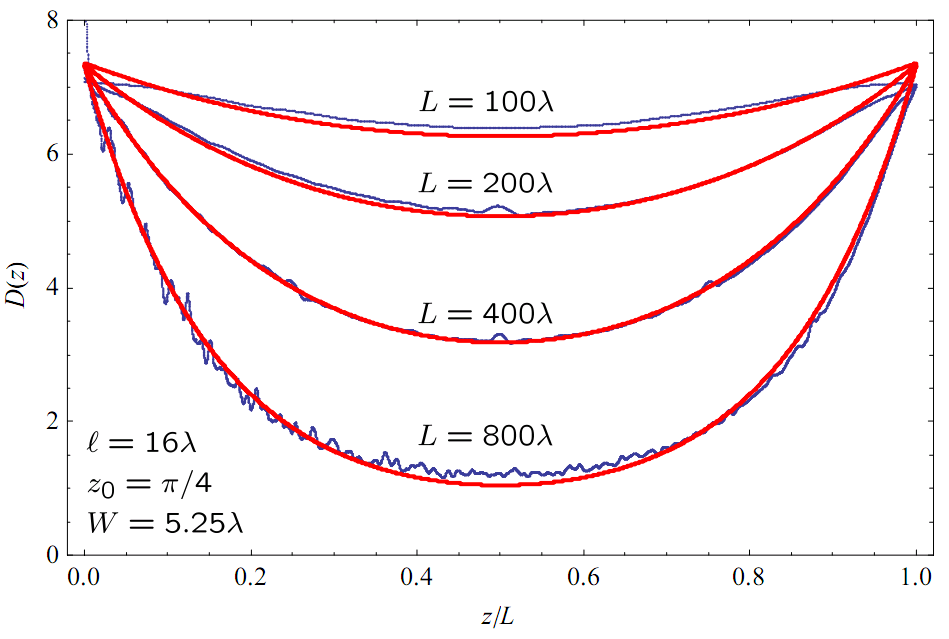
\includegraphics{pictures/Dz_passive}}}
\vskip -0.5cm
% NOTE: if a short caption is needed for figure list, use
%\caption[short desk]{long desk}
\caption[Position-dependent diffusion coefficient~$D(z)$ as predicted by self- consistent theory of localization (smooth red curves) and numeric results (rough blue lines) for quasi-1D waveguides with randomly-placed passive scattering potentials for varying system length~$L$, constant scatterer density, and width~$W$.]{Position-dependent diffusion coefficient $D(z)$ as predicted by self-consistent theory of localization (smooth red curves) and numeric results (rough blue lines) for quasi-1D waveguides with randomly-placed passive scattering potentials for varying system length~$L$, constant scatterer density, and width~$W$. Very good agreement for ballistic ($L=100 \lambda$), diffusive, and localized ($L=800 \lambda$) regimes. The term $\ell$ is transport mean free path, and $z_0$ is penetration depth.}
\label{fig:Dz_passive}
\end{figure}

%Method: How am I numerically modeling these criteria?}
To develop numerical models that can simulate wave transport in nonconservative media for individual realizations of disorder, this work implements the transfer matrix method~\cite{1981_MacKinnon_scaling,1992_Pendry,2003_Kettemann} 
% note: when MacKinnon cites tmm, he uses 1981_MacKinnon_scaling and 
% MacKinnon A 1994 J. Phys. Condensed Matter 6, 2511
for the entire waveguide. Essentially, the transfer matrix method matches boundary conditions before and after an event in a system where wave modes are quantized. Not only is the quasi-1D geometry experimentally viable~\cite{2009_Genack_PRB}, it also provides a convenient theoretical framework~\cite{1982_Dorokhov_DMPK,1988_Mello_Kumar_DMPK}. Here, waveguides described as ``quasi-1D'' have the following characteristics: (1)~quantized transverse modes due to boundary conditions, expressed as $E(y=0,W;\forall z)=0$ as for metallic edges, (2)~waveguide width $W$ less than $\ell_{tmfp}$ so that no significant transverse propagation occurs, and (3)~aspect ratio ($L:W$) is not fixed (i.e., $W$ is constant when $L$ is increased, with a fixed disorder density). Further, the propagation is confined to two dimensions in order to study a single polarization of electromagnetic radiation.

As shown in Appendix~\ref{sec:appendix_derivation_transfer_matrices_quasi1d}, the differential wave equation
\begin{equation}
\nabla^2 E(\vec{r}) = - \frac{\omega^2}{c^2} E(\vec{r})
\label{eq:wave_equation_electric_field_introduction}
\end{equation}
can be separated into perpendicular and parallel components (resolving wave vector $\vec{k}$ into $k_{\perp}$ and $k_{\parallel}$). Once the electric field solution is found, scattering potentials are introduced, initially as $\delta$ functions. The derivation of the transfer matrix method is \textit{ab initio} based on Maxwell's equations~\cite{1999_Jackson}, and no assumption about transport mean free path is made. 

For light waves, transverse wave quantization means that the modes of an electric field and its derivative can be written in the 
form of a vector. The translation of that field in vector form through a dielectric-filled space or past a scattering potential is described by a matrix, the rank of which is dependent on the number of transverse modes of the waveguide (c.f. Appendix~\ref{sec:appendix_derivation_transfer_matrices_quasi1d}). In 1D, the transfer matrix method takes the initial electric field $E_0$ and its derivative $E_0^{\prime}$ and translates to the field and its derivative over distance $\Delta x$:
\begin{equation}
 \left( \begin{array}{cc}
t_{11} & t_{12} \\
t_{21} & t_{22} \\
\end{array} \right)
\left( \begin{array}{c}
E_0 \\
E_0^{\prime}
\end{array} \right)
=
\left( \begin{array}{c}
E_{\Delta x} \\
E_{\Delta x}^{\prime}
\end{array} \right).
\end{equation}
Multiple scattering events are combined as $\hat{T}_{total} = \prod_i \hat{T}_i$. The product describes the effect of the medium on the transport of the incident light. Since the transfer matrices have finite rank, the scattering potentials used are actually a finite summation of Fourier components of the $\delta$ function. Although the purpose of the numerical model is a study of photonic transport in nonconservative media, the resulting electric field magnitude, plotted in Fig.~\ref{fig:electric_field_zoomed}, is a secondary benefit.

\begin{figure}
\vskip -0.5cm
\centerline{
\scalebox{.47}{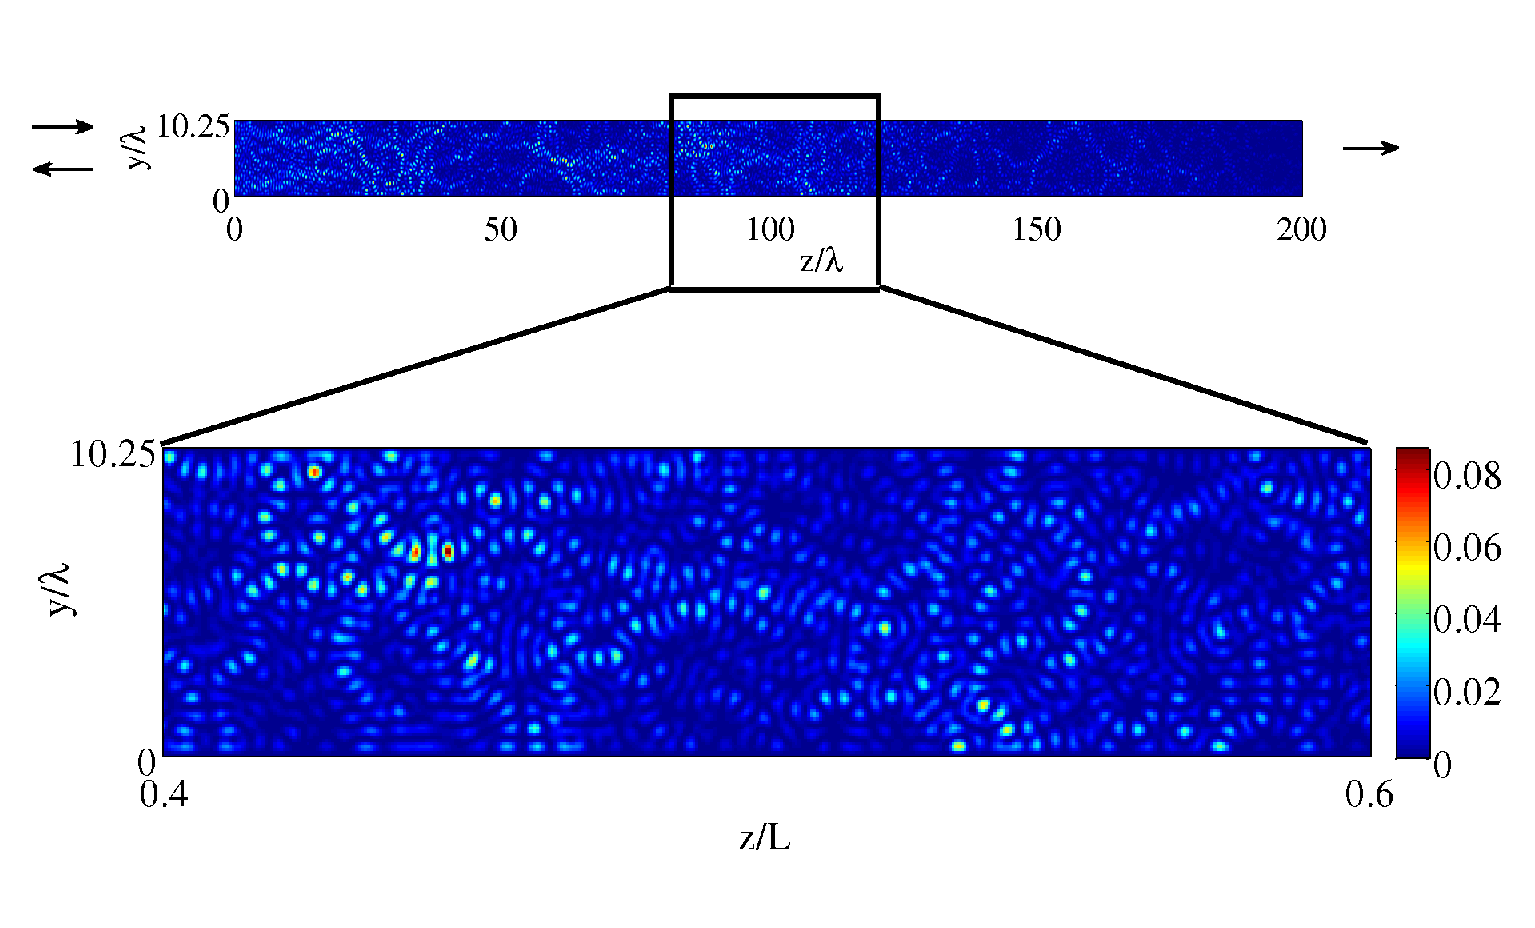
\includegraphics{pictures/electric_field_resonant_freq_zoom_normalized_z_box_arrows}}}
\vskip -0.5cm
% NOTE: if a short caption is needed for figure list, use
%\caption[short desk]{long desk}
\caption[Magnitude of electric field inside a quasi-1D waveguide for passive media in the diffusive regime.]{Magnitude of electric field inside a quasi-1D waveguide for passive media in the diffusive regime. Midsection of waveguide is shown (from $z/L=80/200$ to $z=120/200$) for a resonant frequency (higher than average transmission). Spatially varying field intensity (with continuous wave incident flux) demonstrates interesting microscopic behavior, even though the system is in the diffusive regime.
\label{fig:electric_field_zoomed}}
% The Poynting vector can plotted
% [don't say this because you aren't including a picture of the Poynting vectors.]
\end{figure}

The transfer matrix method is used in the field of transport~\cite{2007_Froufe-Perez_PRE}, but its application is usually limited either to RMT for perturbative study or directly only to the diffusive regime. These limitations are due to the fact that multiplication of numerical matrices results in inaccuracy due to divergent eigenvalues in the product~\cite{1968_Osedelec}.
% A simple showing of this would be nice
The numerical inaccuracy is detectable since each transfer matrix has determinant unity. % (due to conservation of flux?) 
The product of the matrices must retain a determinant of unity since 
%citation would be nice here, but most linear algebra books leave it as an exercise to the reader
%\begin{equation}
$\rm{det}(\hat{A})\rm{det}(\hat{B})=\rm{det}(\hat{A}\hat{B})$.
%\end{equation}
A self-embedding technique renormalizes the divergent eigenvalues and make this approach feasible~\cite{1999_yamilov_selfembed,1976_Bellman_Wing_embedding}.
%Although self-embedding technique applies to any numerical multiplication of many matrices, it is applied here to waveguides. %1D and planar quasi-1D waveguide geometries.
%In passive media, conservation of energy implies $T+R=1$ which is checked for validity of results.
The reliability of the transfer matrix method with self-embedding is demonstrated by comparing numerical simulation results of average unitless conductance $\langle g \rangle$ versus variance var$(g)$ to data yielded by a theoretical supersymmetry-based approach~\cite{2000_Mirlin}. With no fitting parameters, there is very good agreement (c.f. Fig.~\ref{fig:Mirlin_supersymmetry_g_varg}). Similarly, the diffusion coefficient from numerical simulation of passive media matches expected $D(z)$ (c.f. Fig.~\ref{fig:Dz_passive}).

\begin{figure}[t]
\vskip -0.5cm
\centerline{
\scalebox{.5}{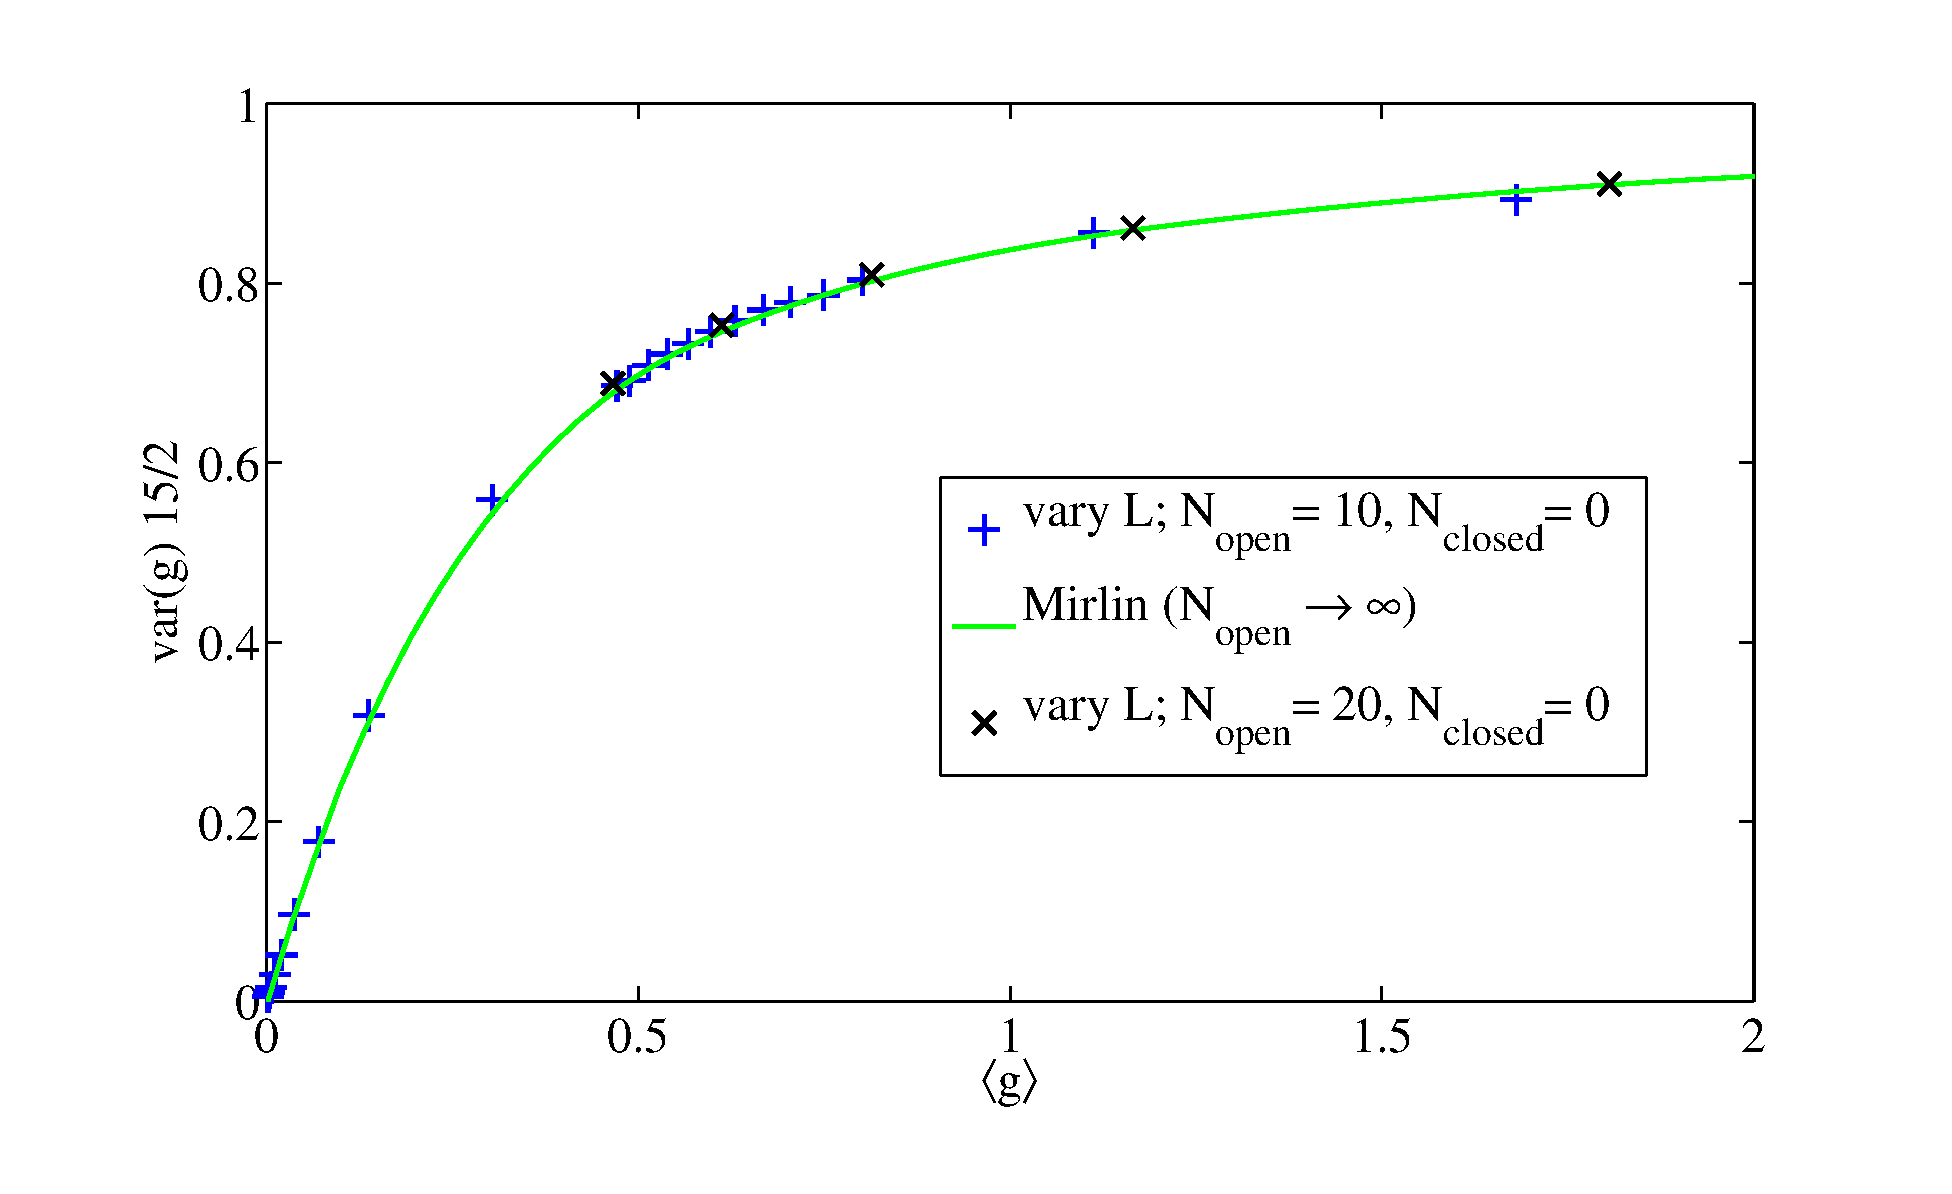
\includegraphics{pictures/var_g_versus_g_no_closed_channels}}}
\vskip -0.5cm
% NOTE: if a short caption is needed for figure list, use
%\caption[short desk]{long desk}
\caption[Theoretical prediction based on supersymmetric approach for average unitless conductance $g$ versus variance of $g$ for quasi-1D waveguide~\cite{2000_Mirlin} compared to results from numerical simulations described in Section~\ref{sec:method_numerical}.]
{Theoretical prediction based on supersymmetric approach for average unitless conductance $g$ versus variance of $g$ for quasi-1D waveguide~\cite{2000_Mirlin} compared to results from numerical simulations described in Section~\ref{sec:method_numerical}. No fitting parameters are used and good agreement is found. The $15/2$ accounts for the geometry of the waveguide. Many realizations of random media for each waveguide determined $\langle g \rangle$ and var$(g)$ for waveguides of two different widths (with the number of open channels $N_{open}$ determined by $W$) and varying system length $L$. The supersymmetry-based approach assumes the limit of an infinite number of propagating modes, but $N_{open}$ equal to 10 and 20 is sufficient.\label{fig:Mirlin_supersymmetry_g_varg}}
\end{figure}
  

\section{OUTLINE OF TRANSPORT REGIMES}
\label{sec:twod_plot}

To guide the study of the extension of the three passive regimes in nonconservative media, a two-parameter diagram (c.f.~Fig.~\ref{fig:regime_plot_main})  % Spring semester 2009, Ben and Dr Yamilov
enumerates types of transport behavior. The first parameter is system length $L$, which varies in relation to constant disorder density and waveguide width for passive media. The second parameter is gain or absorption strength. The two-parameter plot is needed to define specific signatures of diffusion and AL. The chapters that follow use the numerical model of waveguides to verify transitions between types of transport and to characterize behavior of LC such as the proposed $T/{\cal E}$ in nonconservative random media.

A single-valued parameter such as~$T/{\cal E}$ is useful even in this two-parameter space because it indicates only whether diffusion or AL descriptions apply to transport. However, not all single-valued LC are applicable for these systems due to the divergence of most observable parameters as RLT is approached with increased gain. Before determining which side of diffusion or AL is characterized by~$T/{\cal E}$, the behavior on both sides must be defined. Currently, no clear definitions of AL or diffusive behavior exist for nonconservative random media.

%\section{what is the plan?}
Figure~\ref{fig:regime_plot_main} describes types of transport in quasi-1D waveguides with random media; it has three passive regimes: ballistic (\textbf{B}), diffusive (\textbf{D}), localized (\textbf{L}) on the horizontal axis and gain (\textbf{G}) or absorption (\textbf{A}) strength on the vertical axis. The two-letter combinations on the plot denote a regime of specific behavior. The passive regime transitions (B/D/L) are characterized by the transport mean free path~$\ell_{tmfp}$ and localization length~$\xi$, as described in Section~\ref{sec:thesis_statement}. All lengths are normalized by wavelength~$\lambda$. 

\begin{figure}[t]
\vskip -.8cm 
% when scalebox=0.65, -2 gives the figure alone on page, -3cm give no margin at the top.
% when scalebox=0.65, -.8 is figure alone
% when scalebox=0.45, -2 gives not enough margin at top; -.5 and -.8 looks good
\centerline{
\scalebox{.65}{ % 0.65 would be largest
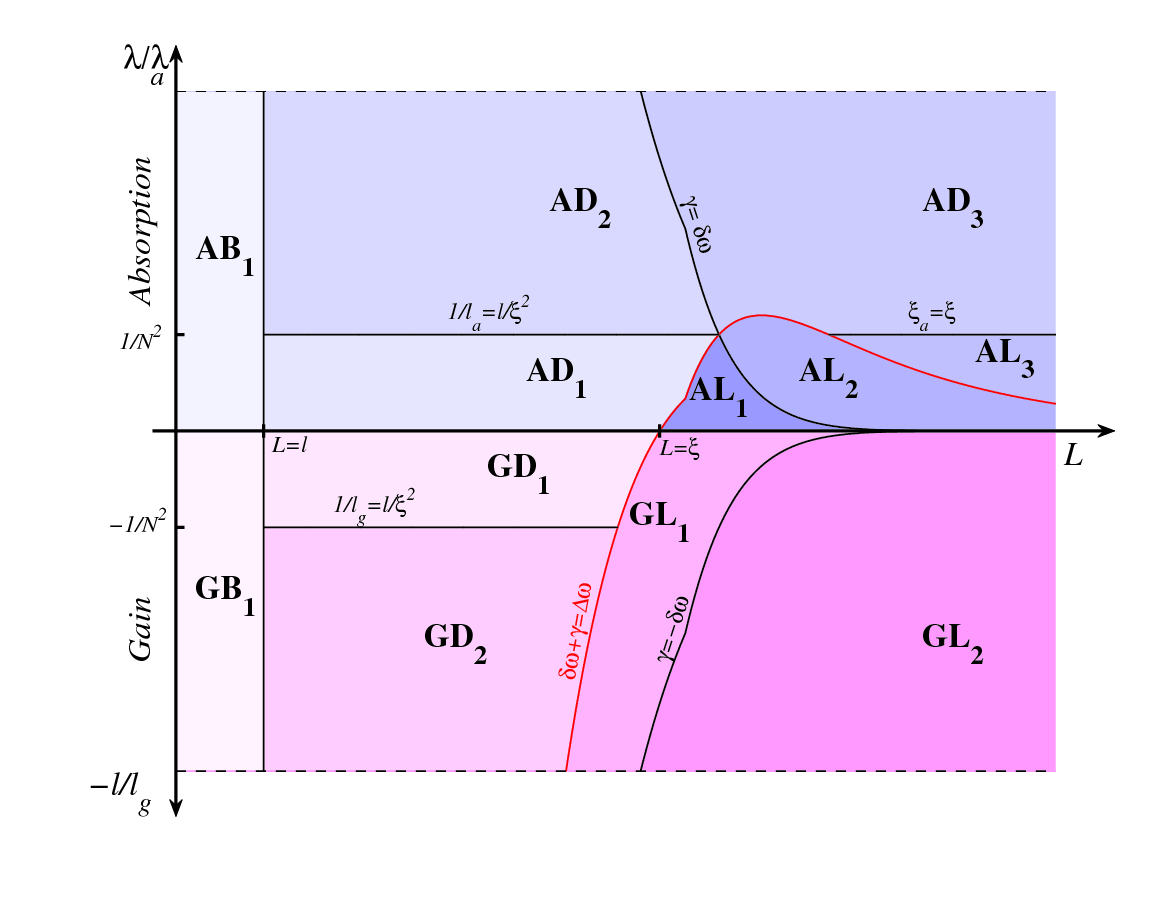
\includegraphics{pictures/regimes_plot_main}}}
\vskip -0.5cm
\caption[Various types of transport phenomena denoted by two-letter abbreviations (see text for explanation).]{Various types of transport phenomena denoted by two-letter abbreviations (see text for explanation). Each region is a permutation of the inequality of relevant characteristic lengths. Passive (conservative) transport regimes are on the horizontal axis, assuming constant disorder density and varying system length $L$. Plotted vertically, amounts of absorption or gain (nonconservative media) increase with distance away from the passive system horizontal axis. 
%Regime plot for quasi-1D random media. Lines denote transitions between regions of similar transport behavior; each region is denoted by a two-letter abbreviation. See text for explanation.
\label{fig:regime_plot_main}
}
\end{figure}

%It is important to note that characteristic lengths are defined in specific regimes. For example, 
%For brevity, only absorption is referred to, but the concepts apply equivalently to gain. 
The absorption (gain) rate $\gamma_{a,g}$ is the average number of absorption events per unit time, where an event refers to the particle removed (doubled) along a specific path. The absorption (gain) rate is the inverse of the absorption (gain) lifetime, 
%\begin{equation}
$\gamma_{a,g} = \frac{1}{\tau_{a,g}}$, 
%\end{equation}
where $\tau_{a,g}$ is the average propagation time of the particle before it is absorbed (doubled). The averaging is over many random particle paths. Given a characteristic time $\tau_{a,g}$, the characteristic absorption or gain length is 
%\begin{equation}
$\ell_{a,g} = \tau_{a,g} c$, 
%\end{equation}
where $c$ is the propagation speed of the particle. This characteristic length is the average distance prior to absorption (doubling) with respect to the path length. The $\ell_{a,g}$ is determined from the time-dependent diffusion equation in one dimension,
\begin{equation}
D \frac{\partial^2 I}{\partial z^2} = \frac{\partial I}{\partial t},
\label{eq:diffusion_equation_1D}
\end{equation}
to be 
% see /svn/bens/lab_notebook/20090422_dr_Yamilov_mtg_regime_change_for_plot.pdf
% equation 37
\begin{equation}
\ell_{a,g}= \left( \frac{d}{\pi^2}\right) \frac{L^2}{\ell_{tmfp}}.
\label{eq:ballistic_gain_abs}
\end{equation}
However, $\ell_{a,g}$ is already defined in the ballistic regime as the average length after which the particle is no longer present in a ballistic system due to absorption (doubled when gain is present). The system length $L$ (how far the particle would have gone along a ballistic path) should be replaced by a new diffusive-regime length, $\xi_{a,g}$. Eq.~\ref{eq:ballistic_gain_abs} can then be solved for $\xi_{a,g}$:
\begin{equation}
 \xi_{a,g} = \sqrt{\frac{\ell_{a,g} \ell_{tmfp}}{d}}.
\label{eq:diffusive_absorption_length}
\end{equation}
Physically, $\xi_{a,g}$ is the average length after which the particle is no longer present in a multiple-scattering system. To distinguish the two absorption (gain) lengths, $\xi_{a,g}$ is measured with respect to system length $L$ (rather than path length $L_D$), whereas $\ell_{a,g}$ is measured with respect to path length $L_D$. If $L$ is equal to $L_D$, then no diffusion is occurring and $\ell_{a,g}$ is equal to $\xi_{a,g}$. Usually, the literature does not distinguish between measurement of an absorption length with respect to diffusive path $L_D$ or measuring it with respect to system length $L$. There are two reasons for this ambiguity: first, experimentally, $L_D$ is harder to measure than $L$; second, the regime to which various lengths apply to is generally not specified.

For localized systems, it no longer makes sense to measure lengths with respect to path length since wave effects are dominant (i.e., ray optics do not apply). In this regime $\xi_{a,g}$ is used, but it is not defined in terms of $\ell_{a,g}$ as in Eq.~\ref{eq:diffusive_absorption_length}. The transition indicating whether or not absorption affects AL or not is set by $\xi_{a} = \xi$ (the horizontal line between $AD_3$ and $AL_3$ in Fig.~\ref{fig:regime_plot_main}). This transition in the diffusive regime is found by applying Eq.~\ref{eq:diffusive_absorption_length} to $\xi_{a,g} = \xi = N_{open} \ell_{tmfp}$ and solving 
\begin{equation}
N_{open}^2 \ell_{tmfp}^2 = \frac{\ell_{tmfp}\ell_{a,g}}{d}
\end{equation}
to get $\ell_{a,g} =d N_{open}^2 \ell_{tmfp}$. For the diffusive regime, this line indicates how much absorption (gain) is necessary to distinguish transport behavior from a passive system. The remaining curves in Fig.~\ref{fig:regime_plot_main} are derived from the density of state transitions, rather than the characteristic lengths.

For passive media, the width of peaks in transmission with respect to frequency ($\delta \omega$ of the Thouless criterion in Eq.~\ref{eq:Thouless_passive}) is inversely proportional to the escape lifetime (the average time until an input leaves the system). To account for absorption or gain, an additional term is needed~\cite{2005_Yamilov_correlations} in the form of a rate: 
%\begin{equation}
$\delta \omega +\gamma_{a,g}$.
%\end{equation}
Although the width of DOS $\Delta \omega$ also changes as a function of gain due to the Kramers-Kronig relation~\cite{1999_Jackson}, the perturbation can be disregarded since the amount of gain and absorption of interest is small. 
% boundaries
The Thouless criterion is adapted to nonconservative media by inclusion of the gain (sometimes referred to as negative absorption~\cite{1968_Letokhov}) or absorption rate $\gamma_{a,g}=\mp~c/\ell_{a,g}$:
\begin{equation}
\delta'=\frac{\delta \omega +\gamma_{a,g}}{\Delta \omega};
\label{eq:generalized_thouless}
\end{equation}
it is plotted as the red curve $\delta'=1$. Physically, this boundary signifies whether the width of quasi-modes or separation of spectral peaks is larger. An additional boundary introduced by inclusion of nonconservative media occurs when absorption or gain overcomes radiative leakage of an average quasi-mode of the system, as plotted by the black curve $\pm \gamma = \delta \omega$. %The remaining boundaries are straight lines and are determined by enumerating permutations of characteristic length scale inequalities. For example, in the diffusive regime, $L$, $\xi$, $\ell_{tmfp}$, and $\ell_{a,g}$ form a minimum basis for distinguishing transport behavior. 
%Enumerating all permutations of relevant length inequalities, a distinct set of transport behaviors has been found.
% caveat
Although each region is separated by a line in Fig.~\ref{fig:regime_plot_main}, the transition between regimes is actually continuous due to the use of many realizations of randomly placed scatterers. Given the boundaries between each region, two-letter abbreviations are defined for each unique transport behavior.

% transport behavior of each regime
In the ballistic regime $GB_1$, gain below ballistic lasing threshold is not expected to change transport behavior (and similarly for $AB_1$ when $\ell_a < L$). For a small amount of absorption or gain in regions $AD_1$ and $GD_1$, the diffusive transport is also expected to remain similar to passive media. The use of conditional statistics~\cite{2005_Yamilov_correlations} eliminates a small number of lasing media. With sufficient absorption, signatures of diffusion are reduced ($AD_2$) and suppressed ($AD_3$). In contrast, gain enhances fluctuations ($GL_1$) and leads to lasing ($GL_2$) on average for many realizations~\cite{1968_Letokhov}. Transport in region $GD_2$ is the equivalent of ``negative absorption'' in region $AD_2$. The remaining absorption regimes signify transition from distinct spectral peaks and leakage due to radiation ($AL_1$) to distinct spectral peaks with absorption dominating leakage ($AL_2$) to a continuous spectrum due to absorption with weak localization ($AL_3$).

% the hump of AL_2 is not separated because?

%The kink in the curves is the transition from diffusion based equations to Mirlin's projections~\cite{2000_Mirlin} in the localized regime.


% if I only have 10 minutes of the presentation, I will not have time for these regions
\begin{comment}
\begin{figure}
\vskip -0.5cm
\centerline{
\scalebox{.75}{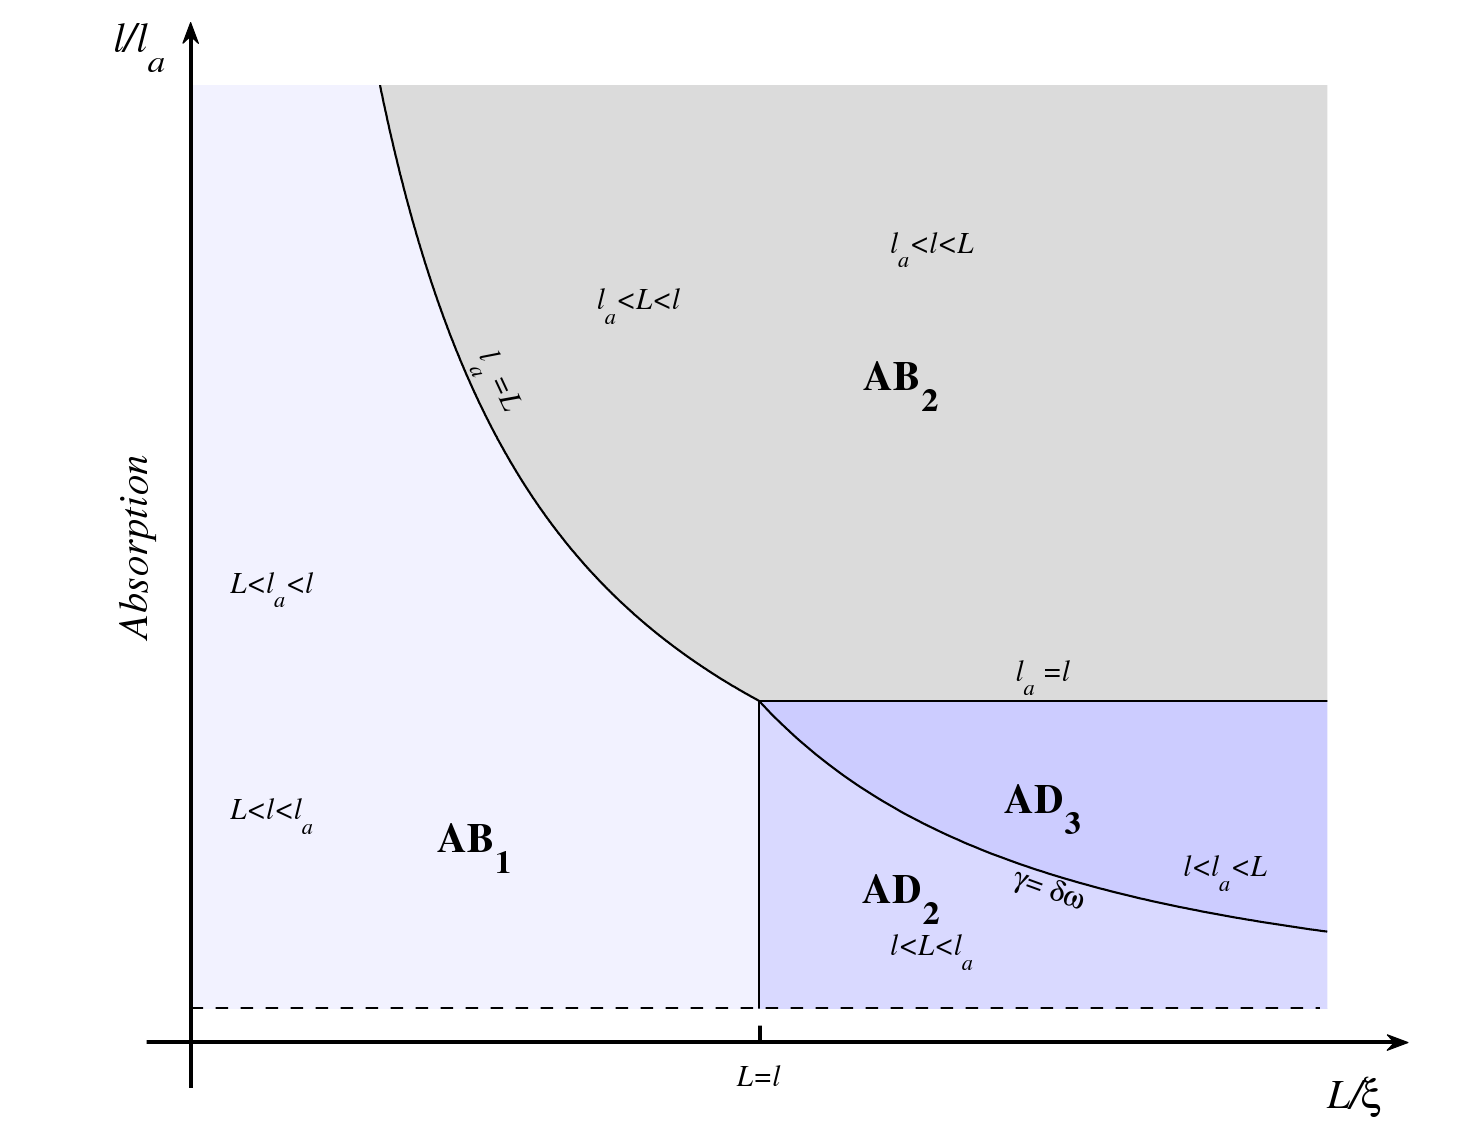
\includegraphics{pictures/regimes_plot_upper}}}
\vskip -0.5cm
%\caption[Upper regime plot (strong absorption) for quasi-1D random media.]{Upper regime plot (strong absorption) for quasi-1D random media. Each region is associated with an inequality of lengths. See text for explanation.}
\label{fig:regime_plot_upper}
\end{figure}

\begin{figure}
\vskip -0.5cm
\centerline{
\scalebox{.75}{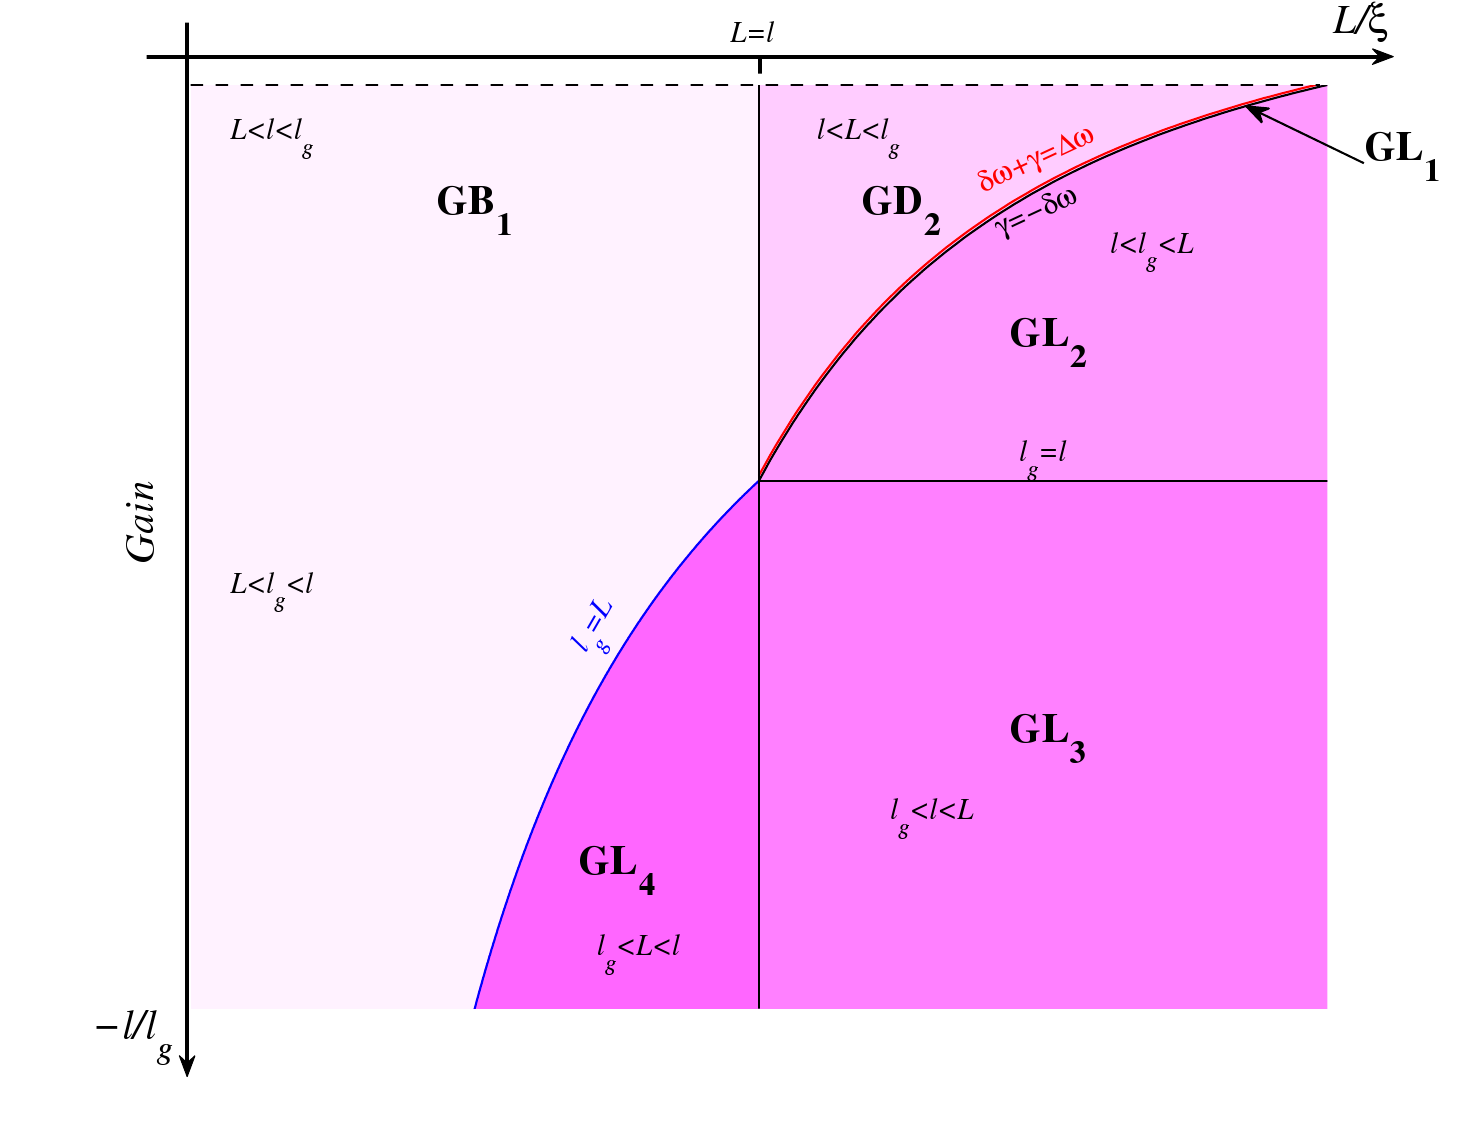
\includegraphics{pictures/regimes_plot_lower}}}
\vskip -0.5cm
%\caption{[Lower regime plot (strong gain) for quasi-1D random media.]Lower regime plot (strong gain) for quasi-1D random media. See text for explanation.}
\label{fig:regime_plot_lower}
\end{figure}
\end{comment}

% Note: analytical quasi-1D solution found by~\cite{1994_Beenakker_exact}

%I expect to be successful because I have sufficient tools (numerical model) and the plan is detailed and well-defined. Also, it is not too broad or too narrow.

To verify the boundaries and transport behaviors specified in Fig.~\ref{fig:regime_plot_main}, the numerical model for waveguides with random media is used to measure the criterion $T/{\cal E}$. In addition to determining the applicability of other LC such as $D(z)$, correlation functions, and the inverse participation ratio, this system makes possible the study of myriad other interesting topics. Examples include the effect of closed channels with gain~\cite{2010_Payne_closed}, wave front shaping~\cite{2008_Vellekoop_Mosk} to change transmission or focus field inside the medium, eigenmodes of transmission~\cite{1986_Imry}, and the visualization of Poynting vector field loops. The numerical model developed serves as a robust method for a comprehensive approach to investigating the transition from diffusion to AL for waveguides with nonconservative random media.

In this dissertation, each of the chapters are either published or in the process of submission to a peer-reviewed journal. Thus each chapter has an abstract, introduction, and conclusion. The first paper, Chapter~\ref{chap:TE_gain}, describes the applicability of the ratio of transmission to energy stored in a random media as a criterion for localization. Although both of these parameters diverge in the presence of optical gain, the ratio for each random medium does not. This criterion is developed in the context of a diffusive slab and also a numerical model of one dimensional layers of dielectric material. Since the lowest dimension for which the transition from diffusion to Anderson localization occurs in quasi-1D, there is a need for how to describe transport regimes with non-conservative media exists. The second paper, Chapter~\ref{chap:regimes}, details the development of boundaries between transport regimes in the two dimensional phase space for random media with gain and absorption. Another complication of the quasi-1D geometry is the inclusion of evanescent channels, which is studied in Chapter~\ref{chap:closed_channels}. We find that the effect of inclusion of evanescent channels is equivalent to renormalizing the transport mean free path. The last paper on random media in this dissertation, Chapter~\ref{chap:Dz_absorb}, demonstrates the validity of the position dependent diffusion coefficient $D(z)$ in the localized regime and in systems with absorption.

The remaining two chapters cover media with correlated disorder. Although random media exhibits unusual behavior, reproducibility is desirable for manufacturing. Thus algorithms specifying the non-random disorder (deterministic aperiodic systems) are of interest. The Thue-Morse pattern has a singular continuous Fourier spectrum, but this does not directly predict what transport properties are expected. In Chapter~\ref{chap:TM_to_TB} a mapping of the two dimensional Thue-Morse pattern is made to the tight-binding model. Then Chapter~\ref{eq:TM_physics} covers the anomalous transport properties, i.e.~coexistence of localized and extended states, exhibited by the Thue-Morse pattern.

\end{ThesisBody}

%ps% ... thesis publications ...
\begin{ThesisPublications}
\PaperManuscript{1}{Relation between transmission and energy stored in random media with gain}
%Phys. Rev. B 82 104204 (2010) doi:10.1103/PhysRevB.82.104204
%/svn/research/Project_1D_Transport/2010_TE_manuscript/2009_TE_prb.tex
% pictures from
%/svn/research/Project_1D_Transport/2010_TE_manuscript/20100115_submission
\setcounter{section}{0}
\setcounter{figure}{0}
\setcounter{table}{0}
\label{paper:1_start}
% \documentclass[aps,prb,superscriptaddress,showpacs,amsmath,amssymb,letterpaper]{revtex4}
% \usepackage{graphicx}
% \usepackage{epsfig,color,verbatim} % multi-line comments
% \usepackage{subfigure}             % allows for use of "sub figure" 1a, 1b, etc
% \usepackage{hyperref}

%\begin{document}

\chapter{Relation between transmission and energy stored in random media with gain}
\label{chap:TE_gain}
\label{paper:1_start}

% \author{Ben Payne$^{1}$, Jonathan Andreasen$^{2}$, Hui Cao$^{2}$, and Alexey Yamilov$^{1}$\footnote{Email: yamilov@mst.edu}\\
\begin{center}
Ben Payne$^1$, Jonathan Andreasen$^2$, Hui Cao$^2$, and Alexey Yamilov$^1$      \label{sec:TE2009}                                                                         \end{center}

\ \\
\begin{center}
\textit{$^1$Department of Physics, Missouri University of Science \& Technology,\\ Rolla, MO 65409\\
$^2$Department of Applied Physics, Yale University, New Haven, CT 06520}\end{center}

\ \\
% {\it $^{1}$Department of Physics, Missouri University of Science \& Technology, Rolla, MO 65409\\
% $^{2}$Department of Applied Physics, Yale University, New Haven, CT 06520}}
% \noaffiliation
% \date{\today}
% \begin{abstract}
\addcontentsline{toc}{section}{ABSTRACT}
\begin{center}\textbf{ABSTRACT\footnote{Published in Physical Review B \textbf{82} 104204 (2010).}}        \end{center}

In this work, we investigate a possibility of using the ratio between optical transmission, $T$, and energy stored inside the system, ${\cal E}$, as a quantitative measure of the enhanced mesoscopic corrections to diffusive transport of light through a random medium with gain. We obtain an expression for $T/{\cal E}$ as a function of amplification strength in the diffusive approximation and show that it does not a have tendency to diverge when the threshold for random lasing is approached, as both $T$ and ${\cal E}$ do. Furthermore, we find that a change in $T/{\cal E}$ signifies a change in the electric field distribution inside the random medium. In the localization regime, we also investigate the correlations between transmission and energy stored in the medium with and without amplification. Our results suggest that $T/{\cal E}$ is a promising parameter which can help characterize the nature of wave transport in random medium with gain.
% \pacs{42.25.Dd,42.55.Zz,72.15.Rn}
% \end{abstract}
% \maketitle 

%\tableofcontents

%%%%%%%%%%%%%%%%%%%%%%%%%%%%%%%%%%%%%%%%%%%%%%%%%%%%%%%%%
\section{INTRODUCTION}
\label{sec:intro}
%%%%%%%%%%%%%%%%%%%%%%%%%%%%%%%%%%%%%%%%%%%%%%%%%%%%%%%%%

Anderson localization \cite{1958_Anderson} (AL) is a wave phenomenon \cite{1960_Ioffe_criterion,1984_John_prl,1985_Anderson} that leads to a breakdown of diffusion\cite{1980_Vollhardt_Wolfle,1991_Altshuler}. First conceived in electronic systems, it originates from  a repeated self-interference of de Broglie waves during their propagation in a random potential. Conservation of number of carriers, enforced because the electrons possess an electric charge, lies in the foundation of the concept of AL. 

Understanding the effect of absorption \cite{1984_John_prl}, ubiquitous in optical systems, turned out to be essential for proper physical description and interpretation of experimental studies of {\it light} localization \cite{1989_Genack,1997_wiersma_nature,1999_Maret,2000_chabanov_nature,2007_Maret,2007_Segev}. It also prompted the search\cite{2000_chabanov_nature} for an alternative criterion of localization in absorbing media. Coherent amplification, which leads to an altogether new physical phenomenon of random lasing\cite{2005_Cao}, demands further refinement of the concept of AL and its criteria in active random media.

In the case of absorption, an alternative criterion, based on the magnitude of {\it fluctuations} of transmission normalized by its average, was put forward \cite{2000_chabanov_nature}. In random media with gain, this quantity (as well as any other statistically averaged quantity) becomes ill-defined \cite{2005_Yamilov_correlations}. This is because there always exists a non-zero probability of encountering a special realization of disorder within the statistical ensemble where the given value of the gain parameter exceeds the threshold for random lasing\cite{2005_Cao}. Without saturation effects, such a realization will have an infinite contribution to a statistical average. Inclusion of the saturation introduces a dependence on system- and material-specific parameters which are not associated with wave-transport properties of the random medium. To avoid such dependence, and at the same time to regularize the statistical ensemble, in Ref. \cite{2005_Yamilov_correlations} we introduced conditional statistics by excluding the diverging contributions. Such an approach indeed turned out to be fruitful in studies of enhanced fluctuations and  correlations in mesoscopic transport of the electromagnetic waves through random medium with optical amplification \cite{2004_Yamilov_intensity,2005_Yamilov_correlations,2006_Yamilov_conductance}. These investigations also motivated us to explore an intriguing possibility of localization by gain -- enhancement of the mesoscopic phenomena with an increase of the amplification strength.

In this work, we investigate the properties of the ratio between transmission $T$ and the energy inside a random medium ${\cal E}$, with the goal of formulating a criterion of AL which would be applicable in the presence of gain. Both parameters should be experimentally accessible in planar systems, e.g. perforated dielectric films, in which the spatial field distribution inside the medium can be obtained via near-field scanning optical microscopy.

In Section~\ref{sec:diffusion_section}, to motivate our choice of the parameter in the form $T/{\cal E}$, we consider random medium in regime of diffusive transport. First we note that when taken separately, both transmission and the energy inside the system ${\cal E}$ exhibit an expected tendency to increase with an increase of the gain strength and to diverge when threshold for random lasing is approached (no saturation mechanism is assumed). However, when taken in a form of a ratio, the divergence is eliminated and the tendency to increase is greatly reduced. Secondly, we show that in passive systems the ratio can be related to the spatially-dependent diffusion constant $D(z)$. The latter concept has been recently invoked \cite{2008_Cherroret,2010_Payne_PRL} in the self-consistent theory of AL to extend the applicability of diffusion approximation into the localized regime. The connection between $T/{\cal E}$ and $D(z)$ demonstrates that the former can, indeed, be used as  a quantitative measure of the contribution of localization (interference) phenomena in transport through disordered systems.

In Section~\ref{sec:diffusion_general} we obtain an expression for $T/{\cal E}$ from the solution of the diffusion equation in a random medium (using the slab geometry) with gain. This establishes a baseline -- a decrease of the parameter $T/{\cal E}$ below the diffusion prediction obtained in this section can be used to quantify the extent to which the gain promotes the localization effects.

In order to further assess the usefulness of $T/{\cal E}$ as a localization criterion, in Sec.~\ref{sec:localization_passive} we also consider random medium in the localized regime where we investigate the correlations between the transmission and stored energy in the same disorder configuration. We show that the ratio strongly depends on the spatial location of localization center. This introduces an additional (geometrical) source of fluctuation which is not present in the transmission coefficient alone. Interestingly, this effect leads to profound gain-induced modification of the electric field distribution inside the system that is studied in Sec.~\ref{sec:localization_gain}. 

Discussion of the obtained results and an outlook is given in Sec.~\ref{sec:discussion_TE}.

%%%%%%%%%%%%%%%%%%%%%%%%%%%%%%%%%%%%%%%%%%%%%%%%%%%%%%%%%
\section{ANALYSIS OF \texorpdfstring{$T/{\cal E}$}{T/E}: DIFFUSIVE REGIME}
\label{sec:diffusion_section}
%%%%%%%%%%%%%%%%%%%%%%%%%%%%%%%%%%%%%%%%%%%%%%%%%%%%%%%%%

\subsection{Model Description}
\label{sec:diffusion_eq}

In weakly scattering random media it is common to disregard the wave nature of carriers (electrons, photons, etc) and to describe the transport in terms of the phase-less diffusion equation. Under this condition, the ensemble-averaged diffusive flux $\langle{\bf J}({\bf r},t)\rangle$ and the energy density $\langle {\cal W}({\bf r},t)\rangle$ are related via\cite{1953_Morse}
\begin{equation}
\langle{\bf J}({\bf r},t)\rangle=-D({\bf r})\boldnabla\langle {\cal W}({\bf r},t)\rangle.
\label{eq:Jflux}
\end{equation}
The diffusion approximation amounts to $D({\bf r})\equiv D_0=v_E \ell/3$, where $\ell$ is transport mean free path and $v_E$ is the energy transport velocity \cite{1991_van_Albada_vE}. In the following we will neglect resonant scattering effects and will assume that $v_E$ is equal to the speed of light in vacuum. 

Vollhardt and W\"{o}lfle \cite{1980_Vollhardt_Wolfle} laid out a theory which allows one to account for wave interference effects while retaining diffusive-like formalism. With recent refinements \cite{2008_Cherroret,2010_Payne_PRL}, it is currently believed that allowing for renormalization and spatial dependence of the diffusion coefficient $D({\bf r})$ provides an adequate description of transport through random medium of finite size even beyond the diffusive regime. At the same time, deviation (reduction) of $D({\bf r})$ from the constant value of $D_0$ is interpreted as a manifestation of the developing localization effects.

Eq.~(\ref{eq:Jflux}) has to be complemented by the energy conservation condition
\begin{equation}
\frac{\partial \langle {\cal W}({\bf r},t)\rangle }{\partial t}+{\rm div}\langle{\bf J}({\bf r},t)\rangle=
\frac{c}{l_g}\langle {\cal W}({\bf r},t)\rangle+J_0 \delta(z-z_p),
\label{eq:Jflux_conserv}
\end{equation}
where $l_g$ is gain length and we assume that the coherent flux of an incident plane wave is converted into diffusive flux $J_0$ at $z=z_p\sim\ell$, the penetration depth \cite{1993_Lisyansky_diffusint}, near the left boundary. The above description can be similarly applied to both for the scalar (e.g. acoustic) waves with ${\cal W}({\bf r},t)=\varepsilon({\bf r})\left|d\psi({\bf r},t)/dt\right|^2/(2c^2)+\left|\boldnabla \psi({\bf r},t)\right|^2/2$ and the electromagnetic waves with ${\cal W}({\bf r},t)=\varepsilon({\bf r})\left|{\bf E}({\bf r},t)\right|^2/2+\mu\left|{\bf H}({\bf r},t)\right|^2/2$ \cite{1953_Morse}. In the former case $c/\varepsilon^{1/2}({\bf r})$ has the physical meaning of local propagation speed of the elastic wave field $\psi({\bf r})$ and in the latter, $\varepsilon({\bf r})$ is the dielectric function and ${\bf E}({\bf r},t)$, ${\bf H}({\bf r},t)$ are the electric and magnetic fields. 

Throughout this work we consider the case of linear gain. Such an approximation is justified for values of gain up to the threshold for random lasing when nonlinear and dynamical effects\cite{2005_Cao,2009_Deych_random_laser_theory,2008_Stone,2008_Conti_opals,2009_Frank} become crucial.

We consider a 3D random medium in the shape of a slab of thickness $L$, where we explicitly  separate the coordinate $z$ normal to the slab from the perpendicular component ${\boldrho}$ as ${\bf r}=({\boldrho},z)$. Under a plane-wave illumination at normal incidence, the dependence on ${\boldrho}$ can be neglected. In this case $J_z(z)$ should be understood as the longitudinal component of the flux per unit of cross-sectional area of the slab.  We will also limit our consideration to a continuous wave (CW) regime where the energy density ${\cal W}(z)$ is stationary: $\partial \langle {\cal W}(z)\rangle/\partial t=0$. Under the above assumptions, the boundary conditions 
\begin{equation}
J_z(z=0)=-J_0R,\ \, J_z(z=L)=J_0T
\label{eq:Jflux_bc}
\end{equation}
together with Eqs.~(\ref{eq:Jflux},\ref{eq:Jflux_conserv}) completely specify the problem.

\subsection{Asymptotic Behavior of \texorpdfstring{$T/{\cal E}$}{T/E}: Passive System Limit}
\label{sec:diffusion_zero_gain}

In Appx.~\ref{app:Dz_derivation} we demonstrate that Eqs.~(\ref{eq:Jflux},\ref{eq:Jflux_conserv},\ref{eq:Jflux_bc}) allow one to obtain the following expression for the ratio between $T$ and ${\cal E}$ in the passive limit $1/l_g\rightarrow 0$:
\begin{equation}
\displaystyle\frac{T}{{\cal E}}\simeq
\displaystyle\frac{1}{J_0} \times
\displaystyle\frac{2D_0}{L^2} \times
\left[
\displaystyle\frac{1}{L}\displaystyle\int_{0}^{L}\displaystyle\frac{D_0}{D(z)}dz
\right]^{-1},
\label{eq:TE_vs_D}
\end{equation}
where the energy stored inside the random medium ${\cal E}$ is formally defined as
\begin{equation}
{\cal E}=\int_0^L\langle {\cal W}(z)\rangle dz.
\label{eq:Energy_definition}
\end{equation}
We note that in the process of deriving Eq.~(\ref{eq:TE_vs_D}), terms on the order of $\sim\ell/L\ll 1$ were dropped.

Eq.~(\ref{eq:TE_vs_D}) establishes a relationship for passive media between the parameter we put forward in this work and the self-consistent diffusion coefficient. As it has been determined theoretically \cite{1980_Vollhardt_Wolfle,2008_Cherroret}, localization effects lead to a steady slow-down of diffusion inside the random medium. Because it results in a monotonic decrease of $T/{\cal E}$ parameter below its diffusion-predicted value, we conclude that the proposed parameter may indeed be used to assess the importance of the localization corrections in wave transport through disordered media.

Neglecting the localization corrections in Eq.~(\ref{eq:TE_vs_D}) by assuming $D(z)\equiv D_0$ gives the expected result
\begin{equation}
\displaystyle\frac{T}{{\cal E}}\simeq
\displaystyle\frac{1}{J_0} \times
\displaystyle\frac{2D_0}{L^2}.
\label{eq:TE_vs_D_simple}
\end{equation}
The quantity $D_0/L^2$ coincides with the reciprocal of diffusion time $t_D$ -- the time required for a pulse to propagate through the slab of random medium. This connection offers a clear physical interpretation of the considered parameter $T/{\cal E}$ as a characteristic time scale of transport through the medium. The reduction of $D(z)<D_0$ leads to a decrease of $T/{\cal E}$, as expected in passive systems.
% BHP, 20120223: the published paper says ``leads to an increase'' but this is incorrect.

\subsection{Asymptotic Behavior of \texorpdfstring{$T/{\cal E}$}{T/E}: Strong Gain Limit}
\label{sec:diffusion_cr_gain}

Under the assumptions specified in Sec.~\ref{sec:diffusion_eq}, the integration of Eq.~(\ref{eq:Jflux_conserv}) over the interval $z\in [0,L]$ with the boundary conditions given by Eq.~(\ref{eq:Jflux_bc}) gives
\begin{equation}
(T+R-1)\times J_0={\cal E}\times (c/l_g).
\label{eq:Jflux_energy_constraint}
\end{equation}
This is essentially an energy conservation condition. Hence, it should be fulfilled in any approximation regardless of whether the interference effects are neglected or fully accounted for. We note that in absence of gain $1/l_g\rightarrow 0$, Eq.~(\ref{eq:Jflux_energy_constraint}) reduces to familiar $T+R=1$ (see Eq.~(\ref{eq:Jflux_bc}) for the definitions of $T,R$).

As we will discuss in detail below in Sec.~\ref{sec:diffusion_general}, close to some critical value of gain length $l_{g,cr}$ the transmission and reflection coefficients tend to diverge. Importantly, because the contribution of the incident flux to the overall energy density is small, $T$ and $R$ become comparable $T\simeq R\gg 1$. Under such conditions, Eq.~(\ref{eq:Jflux_energy_constraint}) yields
\begin{equation}
\displaystyle\frac{T}{{\cal E}}\simeq
\displaystyle\frac{1}{J_0} \times
\displaystyle\frac{c}{2l_g}\rightarrow
\displaystyle\frac{1}{J_0} \times
\displaystyle\frac{c}{2l_{g,cr}}.
\label{eq:Jflux_energy_constraint_cr}
\end{equation}
This shows that the studied ratio $T/{\cal E}$, indeed, remains finite. Its limiting value is directly proportional to the critical gain parameter $1/l_{g,cr}$. In the next section we will obtain an analytical expression for $T/{\cal E}$ at an arbitrary value of gain parameter. It will also help justify the approximations (such as $T\simeq R$ above) made in arriving to the expressions in this and the previous sections -- Eq.~(\ref{eq:Jflux_energy_constraint_cr}) and Eq.~(\ref{eq:TE_vs_D_simple}) respectively.

%%%%%%%%%%%%%%%%%%%%%%%%%%%%%%%%%%%%%%%%%%%%%%%%%%%%%%%%%
\subsection{Intermediate Gains}
\label{sec:diffusion_general}
%%%%%%%%%%%%%%%%%%%%%%%%%%%%%%%%%%%%%%%%%%%%%%%%%%%%%%%%%

In this section, we investigate the effect of amplification on $T/{\cal E}$ for an optically thick ($\ell\ll L$) slab of 3D random medium under assumption specified in Sec.~\ref{sec:diffusion_eq}. We consider a sample with parameters not too close to the Anderson localization transition\cite{1960_Ioffe_criterion}, i.e. $k\ell\gg 1$, so that the condition $D(z)=D_0$ can be reasonably well satisfied. A combination of Eqs.~(\ref{eq:Jflux},\ref{eq:Jflux_conserv}) results in a stationary diffusion equation
\begin{equation}
0=
D_0\nabla_z^2 \langle {\cal W}(z)\rangle+
\frac{c}{l_g}\langle {\cal W}(z)\rangle+J_0 \delta(z-z_p).
\label{eq:diffusion_equation}
\end{equation}
The solution of the diffusion equation for the case of absorption in slab geometry has been obtained in Ref. \cite{1993_Lisyansky_diffusint,1999_van_Rossum}. The related gain solution can be directly inferred through formal substitution $l_a=-l_g$. Such treatment of gain in a scattering problem has become known as the ``negative absorption'' model. It has been successfully used to describe turbid amplifying media such as incoherent random lasers \cite{1968_Letokhov,1994_lawandy_nature,2001_vansoest_thesis}.

The transmission and reflection coefficients can be directly obtained from the solution in Refs.~\cite{1993_Lisyansky_diffusint,1999_van_Rossum} by employing the definition of diffusive flux\cite{1953_Morse}
\begin{equation}
\langle J_{\pm}(z)\rangle = \frac{c}{4} \langle {\cal W}(z)\rangle \mp \frac{D_0}{2} \frac{d\langle {\cal W}(z)\rangle }{dz}
\label{eq:diffusive_flux}
\end{equation}
where $ \langle J_{-}\rangle$ and $ \langle J_{+}\rangle $ are the fluxes propagating along negative and positive $z$-directions respectively. Evaluating $\langle J_{-}(0)\rangle$ and $\langle J_{+}(L)\rangle$ we find the following expressions for reflected and transmitted fluxes
\begin{eqnarray}
\langle J_- (0)\rangle  = J_0 \frac{\sin(\alpha  (L-z _p)) + \alpha z_0 \cos(\alpha (L-z _p))}{(1-\alpha ^2 z_0 ^2) \sin(\alpha L) + 2 \alpha z_0 \cos(\alpha L)}
\label{eq:Jreflectionflux} \\
\langle J_+ (L)\rangle  = J_0 \frac{\sin(\alpha z_p) + \alpha z _0 \cos(\alpha z_p)}{(1-\alpha^2 z_0^2) \sin(\alpha L) + 2 \alpha z_0 \cos(\alpha L)},
\label{eq:Jtransmissionflux}
\end{eqnarray}
where $z_0=2\ell/3\sim\ell$ is the extrapolation length \cite{1991_zhu_z0}, and $\alpha^{-1}=\sqrt{\ell l_g/3}$. Ensemble-averaged electromagnetic energy inside the sample can be also determined by integrating the energy density over the entire system, c.f.~Eq.~(\ref{eq:Energy_definition})
%\begin{widetext}
\begin{equation}
{\cal E}=
\frac{J_0}{D_0 \alpha ^2} \left[\frac
{\sin(\alpha z_p) + \sin(\alpha (L-z_p))+\alpha z_0 (\cos(\alpha z_p) + \cos(\alpha (L-z_p))}
{(1-\alpha^2 z_0^2)\sin(\alpha L)+2\alpha z_0\cos(\alpha L)}-1\right].
\label{eq:diffusive_energy}
\end{equation}
%\end{widetext}
It is easy to verify that energy conservation Eq.~(\ref{eq:Jflux_energy_constraint}) is satisfied.

% %%%%%%%%%%%%%%%%%%%%%%%%%%%%%%%%%%%%%%%
% \begin{figure}
% \centerline{\rotatebox{0}{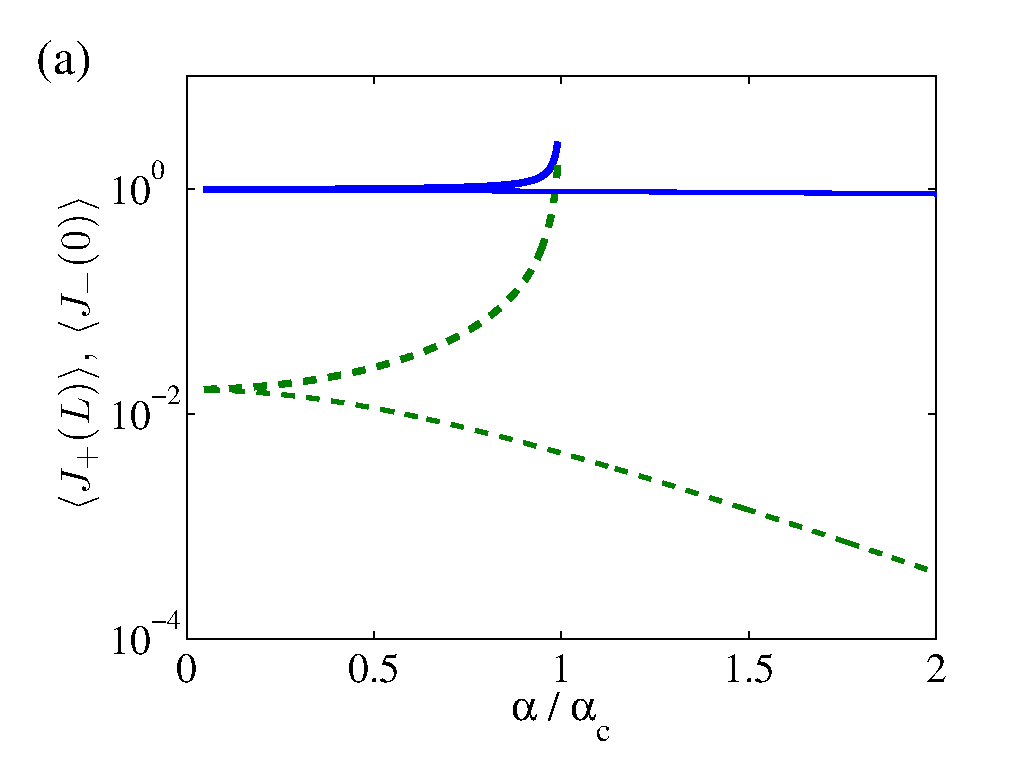
\includegraphics[width=3in]{chapters/Relation_between_transmission_and_energy_stored_in_random_media_with_gain__Phys_Rev_B/pictures/fig1a_yamilov_fixed_L_variable_gain_R_T}}}
% \centerline{\rotatebox{0}{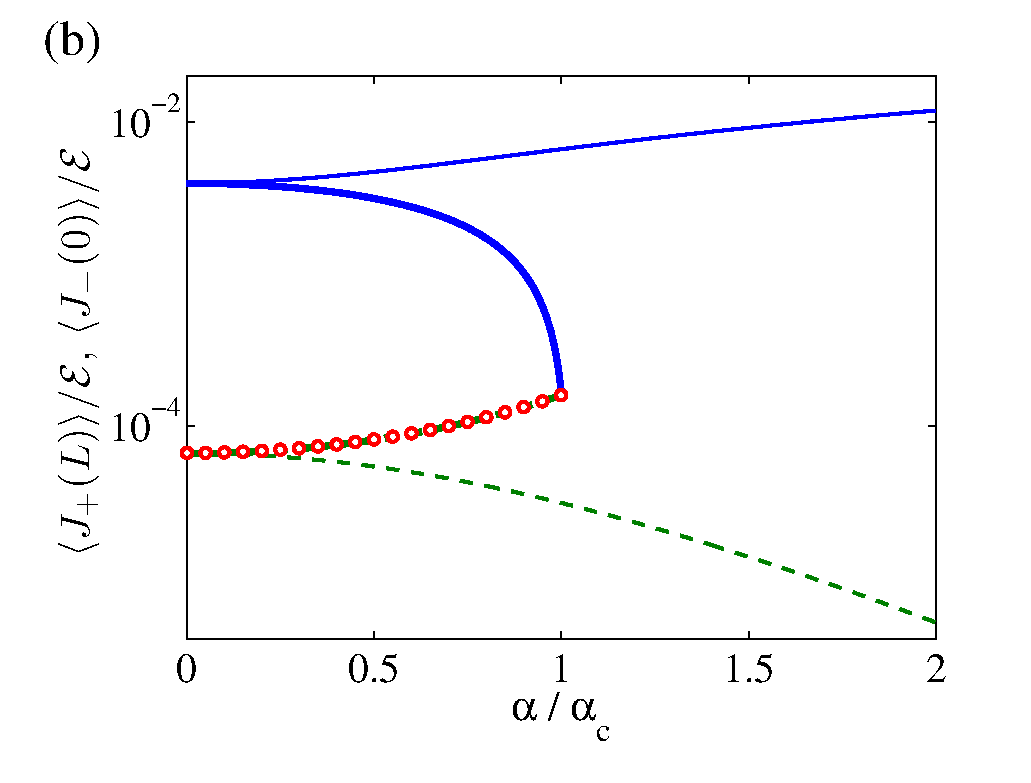
\includegraphics[width=3in]{chapters/Relation_between_transmission_and_energy_stored_in_random_media_with_gain__Phys_Rev_B/pictures/fig1b_yamilov_fixed_L_variable_gain_R_T_divided_by_Energy}}}
% \centerline{\rotatebox{0}{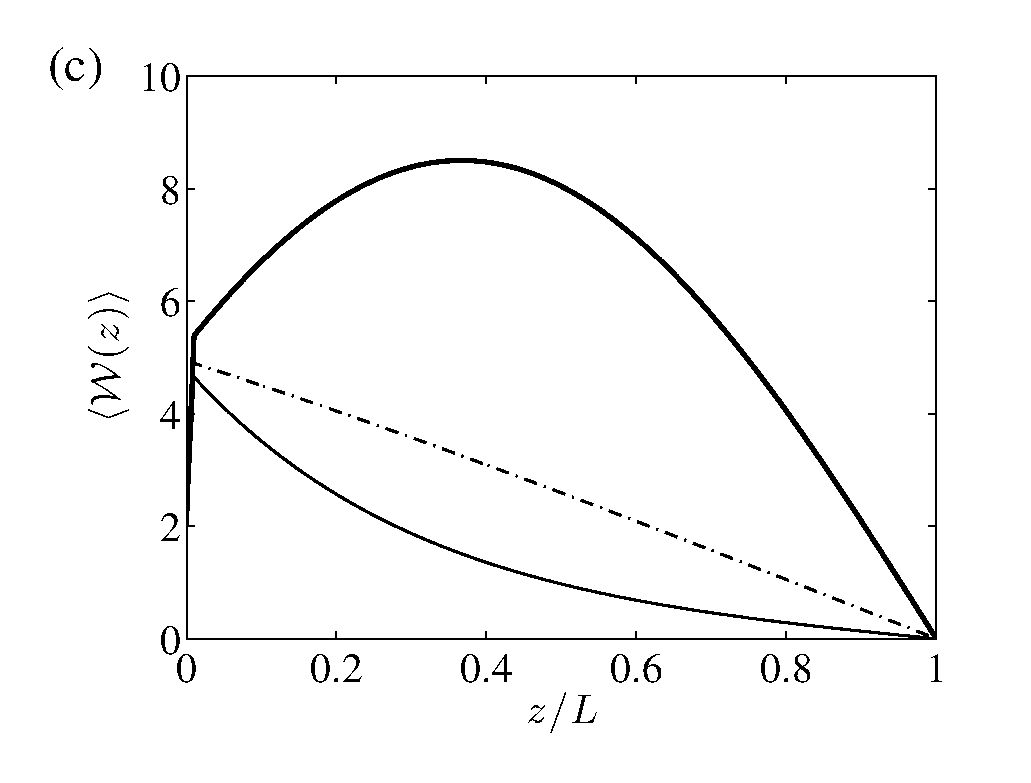
\includegraphics[width=3in]{chapters/Relation_between_transmission_and_energy_stored_in_random_media_with_gain__Phys_Rev_B/pictures/fig1c_yamilov_diffusive_intensity_distribution}}}
% \vskip -.5cm
% \caption[(a) Transmission $ \langle J_{+}(L)\rangle $ (dashed line) and reflection $ \langle J_{-}(0)\rangle$ (solid line) given by Eqs.~(\ref{eq:Jreflectionflux},\ref{eq:Jtransmissionflux}) are plotted for increasing gain (thick lines) and absorption (thin lines) coefficients for a slab of random medium of thickness $L/\ell =100$.]{(a) Transmission $ \langle J_{+}(L)\rangle $ (dashed line) and reflection $ \langle J_{-}(0)\rangle$ (solid line) given by Eqs.~(\ref{eq:Jreflectionflux},\ref{eq:Jtransmissionflux}) are plotted for increasing gain (thick lines) and absorption (thin lines) coefficients for a slab of random medium of thickness $L/\ell =100$. In panel (b) we plot the same quantities as in (a) but normalized by the value of total energy stored inside random medium ${\cal E}$, c.f.~Eq.~(\ref{eq:diffusive_energy}). The divergence in the vicinity of RLT is prevented as both curves approach the same limiting value given by Eq.~(\ref{eq:Jflux_energy_constraint_cr}). $T/{\cal E}$ obtained by evaluating the approximate expression Eq.~(\ref{eq:TE_analytical}) is shown with open circles. For the chosen $L/\ell=100\gg1$ the deviation from the exact result is indiscernible. (c) Diffuse energy density distribution $\langle {\cal W}(z)\rangle$ inside the slab of random medium with thickness $L/\ell=100$ from Eq.~(\ref{eq:diffusive_energy}). Thick solid line corresponds to the sample with gain ($\alpha/\alpha_{cr}=0.8$), dashed line -- to passive sample, whereas thin solid line -- to the sample with absorption($\left|\alpha/\alpha_{cr}\right|=1$). Absorption curve is shown for comparison.\label{fig:diffusive_TE}}
% \end{figure}
% %%%%%%%%%%%%%%%%%%%%%%%%%%%%%%%%%%%%%%%

%%%%%%%%%%%%%%%%%%%%%%%%%%%%%%%%%%%%%%%
\begin{figure}
\centerline{\rotatebox{0}{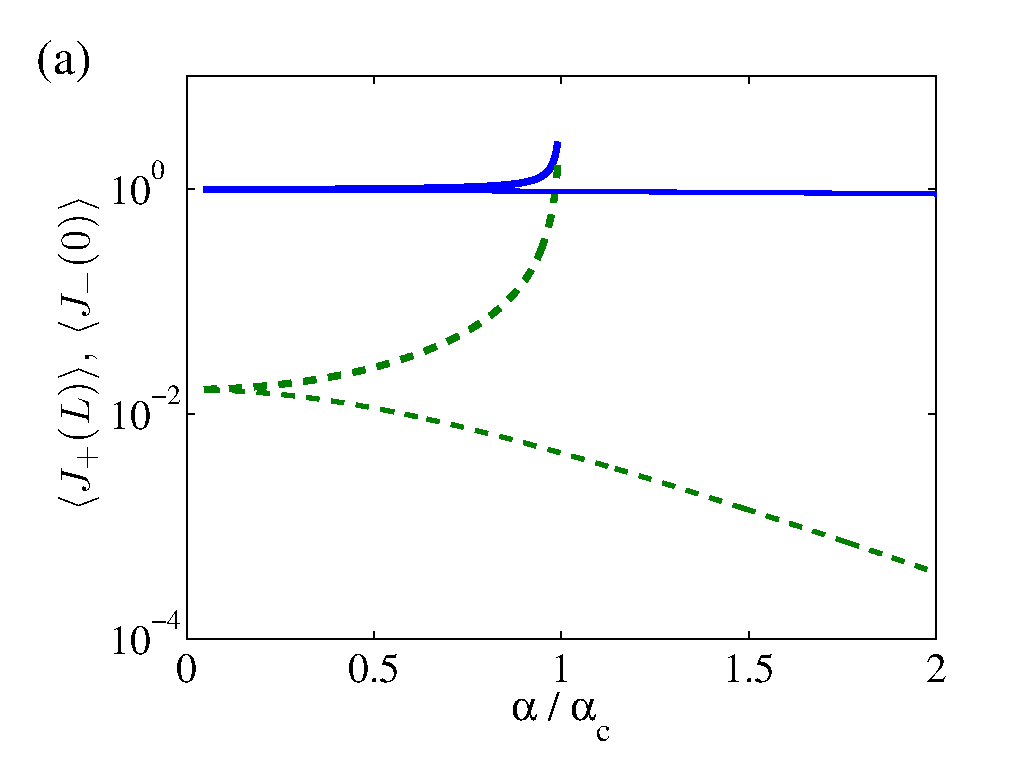
\includegraphics[width=4.5in]{chapters/Relation_between_transmission_and_energy_stored_in_random_media_with_gain__Phys_Rev_B/pictures/fig1a_yamilov_fixed_L_variable_gain_R_T}}}
\centerline{\rotatebox{0}{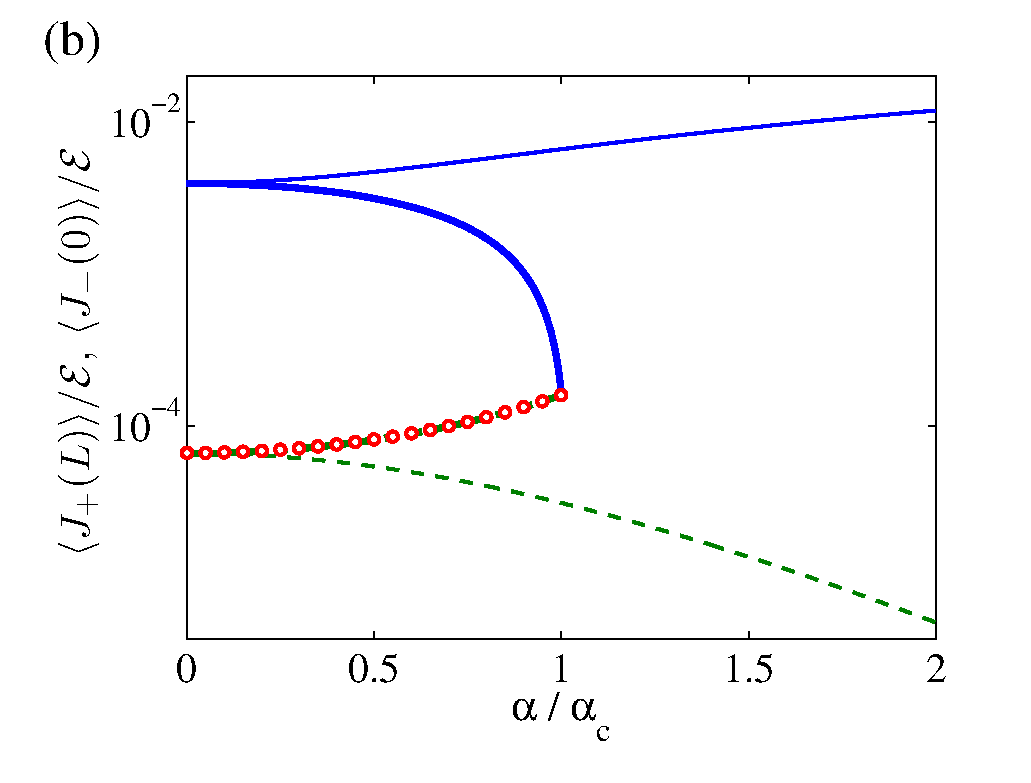
\includegraphics[width=4.5in]{chapters/Relation_between_transmission_and_energy_stored_in_random_media_with_gain__Phys_Rev_B/pictures/fig1b_yamilov_fixed_L_variable_gain_R_T_divided_by_Energy}}}
\caption[(a) Transmission $ \langle J_{+}(L)\rangle $ (dashed line) and reflection $ \langle J_{-}(0)\rangle$ (solid line) given by Eqs.~(\ref{eq:Jreflectionflux},\ref{eq:Jtransmissionflux}) are plotted for increasing gain (thick lines) and absorption (thin lines) coefficients for a slab of random medium of thickness $L/\ell =100$.]{(a) Transmission $ \langle J_{+}(L)\rangle $ (dashed line) and reflection $ \langle J_{-}(0)\rangle$ (solid line) given by Eqs.~(\ref{eq:Jreflectionflux},\ref{eq:Jtransmissionflux}) are plotted for increasing gain (thick lines) and absorption (thin lines) coefficients for a slab of random medium of thickness $L/\ell =100$. In panel (b) we plot the same quantities as in (a) but normalized by the value of total energy stored inside random medium ${\cal E}$, c.f.~Eq.~(\ref{eq:diffusive_energy}). The divergence in the vicinity of RLT is prevented as both curves approach the same limiting value given by Eq.~(\ref{eq:Jflux_energy_constraint_cr}). $T/{\cal E}$ obtained by evaluating the approximate expression Eq.~(\ref{eq:TE_analytical}) is shown with open circles. For the chosen $L/\ell=100\gg1$ the deviation from the exact result is indiscernible.
\label{fig:diffusive_TE_ab}}
\end{figure}

\begin{figure}
\centerline{\rotatebox{0}{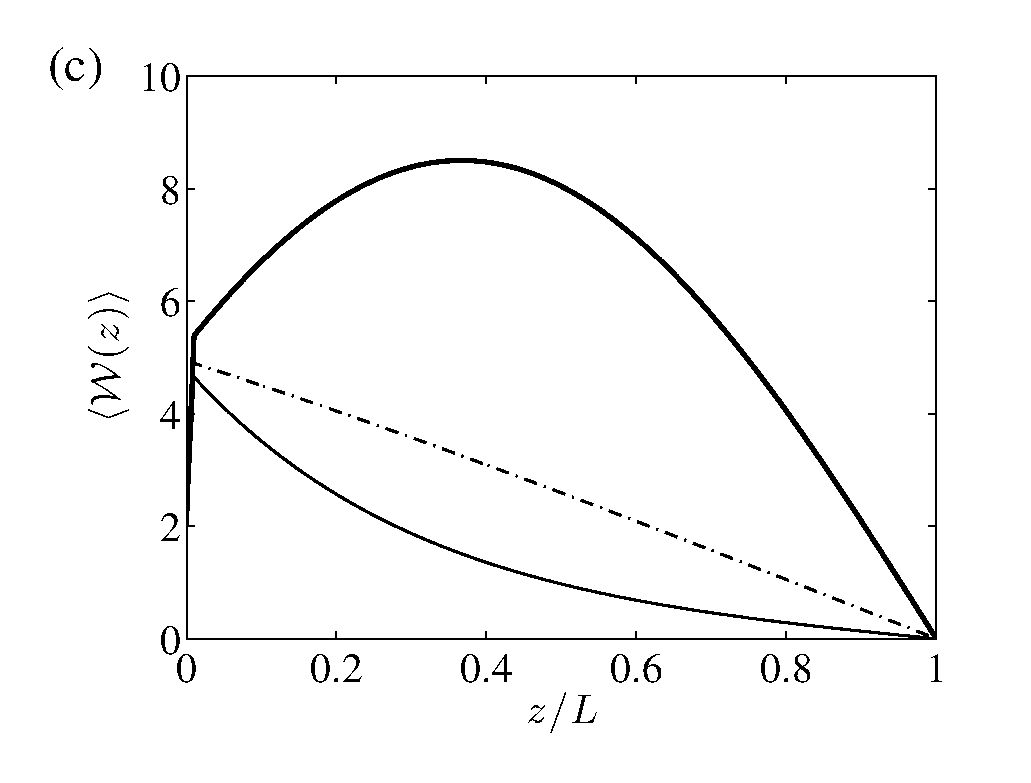
\includegraphics[width=3in]{chapters/Relation_between_transmission_and_energy_stored_in_random_media_with_gain__Phys_Rev_B/pictures/fig1c_yamilov_diffusive_intensity_distribution}}}
\vskip -.5cm
\caption[Diffuse energy density distribution $\langle {\cal W}(z)\rangle$ inside the slab of random medium with thickness $L/\ell=100$ from Eq.~(\ref{eq:diffusive_energy}).]{Diffuse energy density distribution $\langle {\cal W}(z)\rangle$ inside the slab of random medium with thickness $L/\ell=100$ from Eq.~(\ref{eq:diffusive_energy}). Thick solid line corresponds to the sample with gain ($\alpha/\alpha_{cr}=0.8$), dashed line -- to passive sample, whereas thin solid line -- to the sample with absorption($\left|\alpha/\alpha_{cr}\right|=1$). Absorption curve is shown for comparison.
\label{fig:diffusive_TE_c}}
\end{figure}
%%%%%%%%%%%%%%%%%%%%%%%%%%%%%%%%%%%%%%%

In Fig.~\ref{fig:diffusive_TE_ab}a,b we plot Eqs.~(\ref{eq:Jreflectionflux},\ref{eq:Jtransmissionflux},\ref{eq:diffusive_energy}) for a slab of thickness $L/\ell=100$. As expected, we observe the divergence of the transmission and reflection fluxes, c.f.~Fig.~\ref{fig:diffusive_TE_ab}a, when diffusive random lasing threshold (RLT) is approached ($\alpha\rightarrow\alpha_{cr}=\pi/(L+2z_0)\simeq \pi/L$) with an increase of gain parameter $\alpha$ or, equivalently, a decrease of gain length $l_g$ toward $l_{g,cr}\simeq 3L^2/(\pi^2\ell)$. The asymptotic dependence is then
\begin{equation}
\langle J_- (0)\rangle \simeq \langle J_+ (L)\rangle \simeq J_0\frac{z_0 +
z_p}{\pi} \frac{\alpha_{cr} ^2}{\alpha_{cr} -\alpha}.
\label{eq:tr_near_threshold}
\end{equation}
Similar critical behavior is obtained when the system size $L$ is increased towards critical length, $L_{cr}(\alpha)$,while keeping the gain parameter $\alpha$ fixed.

In Fig.~\ref{fig:diffusive_TE_ab}b we also plot the ratios of reflection to energy $\langle J_- (0)\rangle /{\cal E}\equiv J_0R/{\cal E}$ and transmission to energy $\langle J_+ (L)\rangle /{\cal E}\equiv J_0T/{\cal E}$ obtained from Eqs.~(\ref{eq:Jreflectionflux},\ref{eq:Jtransmissionflux},\ref{eq:diffusive_energy}). One can observe that both $R/{\cal E}$ and $T/{\cal E}$ indeed remain finite at $\alpha_{cr}$ with the same limiting value given by Eq.~(\ref{eq:Jflux_energy_constraint_cr}). Although the leading terms in Laurent series in powers of $(\alpha_{cr} -\alpha )$, Eq.~(\ref{eq:tr_near_threshold}), are same for both reflection and transmission, the second order terms (not shown) are not. This explains different slopes of $R/{\cal E}$ and $T/{\cal E}$ in approach to lasing threshold in Fig.~\ref{fig:diffusive_TE_ab}b.

By making assumption that $\ell/L\ll 1$, we find a compact analytical expression for $T/{\cal E}$ with {\it an arbitrary value of gain parameter} $\alpha$: 
\begin{equation}
\frac{T}{{\cal E}} \simeq \displaystyle\frac{D_0\alpha^2}{2J_0\sin^2\left(\alpha L/2\right)}.
\label{eq:TE_analytical}
\end{equation}
Fig.~\ref{fig:diffusive_TE_ab}b shows that this approximate expression (open circles) gives an excellent agreement with the exact results of Eqs.~(\ref{eq:Jtransmissionflux},\ref{eq:diffusive_energy}). It is also easy to check that the limiting expressions of $T/{\cal E}$ Eqs.~(\ref{eq:TE_vs_D_simple},\ref{eq:Jflux_energy_constraint_cr}) obtained in the previous sections follow immediately from the above expression.

%For brevity we will refer to these quantities as $\langle R \rangle / \langle{\cal E}\rangle$  and $\langle T \rangle / \langle{\cal E}\rangle$. 

Based on our observations above, we make the following conclusions that will also inform our investigations in the following Sec.~\ref{sec:localization_passive}:\\
(a) Sufficiently close to the lasing threshold, the reflection and transmission fluxes diverge and become almost equal, c.f.~Eq.~(\ref{eq:tr_near_threshold}). This signifies the fact that the system approaches the regime when the gain alone can sustain its energy, without relying on the incident flux;\\
(b) When normalized by the total energy in the slab defined by Eq.~(\ref{eq:Energy_definition}), both $R/{\cal E}$  and $T/{\cal E}$ do not diverge when the RLT is approached. Instead, they converge to the finite value of $c/(2l_{g,cr})\equiv 2D_0/L^2\times (\pi^2/4)$, c.f.~Eq.~(\ref{eq:Jflux_energy_constraint_cr}). Note that the effect of gain is to increase this parameter by a factor $\pi^2/4\simeq 2.5$ compared to the value in the passive system,~c.f.~Eq.~(\ref{eq:TE_vs_D_simple});\\
(c) The change of the quantities $R/{\cal E}$ and $T /{\cal E}$ is related to modification of the intensity distribution inside the volume of random medium, c.f.~Fig.~\ref{fig:diffusive_TE_c}c. When energy density $\langle {\cal W}(z)\rangle$ assumes the limiting profile given by the lowest order diffusion mode $\langle {\cal W}(z)\rangle\propto\sin(\pi z/L)$ the ratios $R/{\cal E}$  and $T/{\cal E}$ saturate;\\
(d) In Sec.~\ref{sec:diffusion_zero_gain} we showed, c.f.~Eq.~(\ref{eq:TE_vs_D}), that wave interference effects in passive system tend to make the parameter $T/{\cal E}$ smaller then its diffusion prediction, Eq.~(\ref{eq:TE_vs_D_simple}). We expect the same trend to continue in random media with gain. Thus, Eq.~(\ref{eq:TE_analytical}) plays an important role as it establishes a baseline, with downward deviations from which  may be attributed to the enhancement of the wave phenomena.

As we are interested in the interplay between the effects of gain and light localization, in the following we acknowledge the limitations of the diffusive description of this section:\\
(i) The diffusion approximation (no renormalization of diffusion coefficient is assumed) fails when wave phenomena such as localization or coherent random lasing become important. Proper treatment of electric field and its phase becomes necessary;\\
(ii) Increase in gain or scattering strength is expected to lead to an increase of fluctuations of both transport coefficients \cite{2005_Yamilov_correlations} and random lasing threshold \cite{1995_zyuzin_fluctuations}. Thus $T/{\cal E}$ in the form of a ratio between the {\it average} values of two quantities will no longer adequately represent the ratio between the transmission $\tilde{T}$ and energy-stored $\tilde{\cal E}$ in any given realization. Instead, it may need to be replaced with $\langle \tilde{T}/\tilde{\cal E}\rangle$ which would account for correlation between two quantities in the same sample;\\
(iii) With further increase of gain toward RLT, the divergence of fluctuations of $\tilde{T}$ may necessitate the consideration of higher moments $\left\langle \left(\tilde{T}/\tilde{\cal E}\right)^n\right\rangle$ or, perhaps, its entire distribution; \\
(iv) At the onset of random lasing, nonlinear and dynamical processes\cite{2005_Cao,2009_Deych_random_laser_theory,2008_Stone,2008_Conti_opals,2009_Frank} become essential for proper description of the system properties and, thus, a CW quantity such as $T/{\cal E}$ may no longer be suitable.

%%%%%%%%%%%%%%%%%%%%%%%%%%%%%%%%%%%%%%%%%%%%%%%%%%%%%%%%%
\section{ANALYSIS OF \texorpdfstring{$T/{\cal E}$}{T/E}: LOCALIZED REGIME}
\label{sec:localization_passive}
%%%%%%%%%%%%%%%%%%%%%%%%%%%%%%%%%%%%%%%%%%%%%%%%%%%%%%%%%

%%%%%%%%%%%%%%%%%%%%%%%%%%%%%%%%%%%%%%%%%%%%%%%%%%%%%%%%%
\subsection{Model Description}
\label{sec:numerical_model}
%%%%%%%%%%%%%%%%%%%%%%%%%%%%%%%%%%%%%%%%%%%%%%%%%%%%%%%%%

In this section we investigate how fluctuations effects (i-iii) from Sec.~\ref{sec:diffusion_general} influence $\tilde{T}/\tilde{\cal E}$. We remind that the tilde is used to denote the transmission and stored energy in the given sample whereas $T$ and ${\cal E}$ are reserved for the ensemble-averaged quantities. Compared to Sec.~\ref{sec:diffusion_section}, we consider the other extreme case -- the regime of localized transport -- where the fluctuations play the dominant role even in a passive system. For this purpose a one-dimensional (1D) model is already sufficient. Indeed, long enough 1D systems are necessarily in localized regime and, therefore, the fluctuation effects will be essential even at small values of gain. Despite the reduced dimensionality, there are a number of experimental systems \cite{2006_Genack_1d,2006_Scales,2008_LunaAcosta,2005_Genack_Milner} for which the considered one-dimensional model is applicable directly.

We consider a passive system having alternating layers of dielectric material ($\epsilon =$ 1 and 1.2), and width $a$. %, c.f.~Fig.~\ref{fig:dimaSetup}. 
% NOTE: fig:dimaSetup is commented out
This pair of layers is repeated to create 1000 pairs. One last $\epsilon = 1$ layer is added to the end to create a stack of 2001 layers. Then the total sample has length L. Randomness is introduced by varying the width of each $\epsilon=1.2$ layer. The disorder strength and frequency range are chosen so that the system is in the regime of locally weak disorder ($a\ll\xi$); the localization length $\xi\sim L/5$ to $L/10$, and single parameter scaling is applicable\cite{2000_Deych_sps}. Gain or absorption can be included via the imaginary part of the dielectric constant.

We consider an electromagnetic wave of unit magnitude incident on the system. We will distinguish between the cases when the wave is incident from the left and from the right, as defined by the following asymptotic behavior of the electric field:
\begin{eqnarray}
&\left\{
\begin{array}{l l}
E_L(x<0,\omega)=\exp[i\omega x/c]+r_L(\omega)\exp[-i\omega x/c]\\
E_L(x>L,\omega)=t_L(\omega)\exp[i\omega x/c]\\
\end{array} \right. \label{eq:basis_functions_bc_l}\\
&\left\{
\begin{array}{l l}
E_R(x<0,\omega)=t_R(\omega)\exp[-i\omega x/c]\\
E_R(x>L,\omega)=\exp[-i\omega x/c]+r_R(\omega)\exp[i\omega x/c]\\
\end{array} \right. \label{eq:basis_functions_bc_r}
\end{eqnarray}
Here, $r_{L,R}(\omega),t_{L,R}(\omega)$ are the corresponding amplitude reflection and transmission coefficients; $\tilde{T}=\left|t\right|^2$ and $\tilde{R}=\left|r\right|^2$. Wave propagation through the system is modeled using $2\times 2$ transfer matrices\cite{1994_Pendry,2005_Yeh_book,2004_Mello_Kumar_book} 
\begin{equation}
\widehat{t}_i=\left[
\begin{array}{cc}
\cos(k n_i a_i) & n_i^{-1}\sin(k n_i a_i) \\
-n_i \sin(k n_i a_i) & \cos(k n_i a_i)
\end{array}
\right]
\label{eq:transfer_matrix}
\end{equation}
which act on the two-element vector expressing the values of the electric field and its derivative taken at the boundary between the dielectric slabs. Here $n_i=\epsilon_i^{1/2}$ is the refractive index and $a_i$ is the width of the $i'$th slab.

We use this numerical model to simulate CW response of the random system within  certain spectral range. Fig.~\ref{fig:electricFieldInSample} shows a typical distribution of electric field inside random medium and the corresponding transmission and energy ${\cal E}$ obtained in a single realization. Subsequently, this simulation is repeated for a number of random configurations. In Sections~\ref{sec:correlation_te}--\ref{sec:spectral_te} the system is assumed to be passive. The effect of linear gain is considered in Section~\ref{sec:localization_gain}.

%%%%%%%%%%%%%%%%%%%%%%%%%%%%%%%%%%%%%%%
\begin{figure}
\vskip -1in
\centerline{\rotatebox{0}{\includegraphics[width=5in]{chapters/Relation_between_transmission_and_energy_stored_in_random_media_with_gain__Phys_Rev_B/pictures/fig2a_electric_field_in_sample}}}
\centerline{\rotatebox{0}{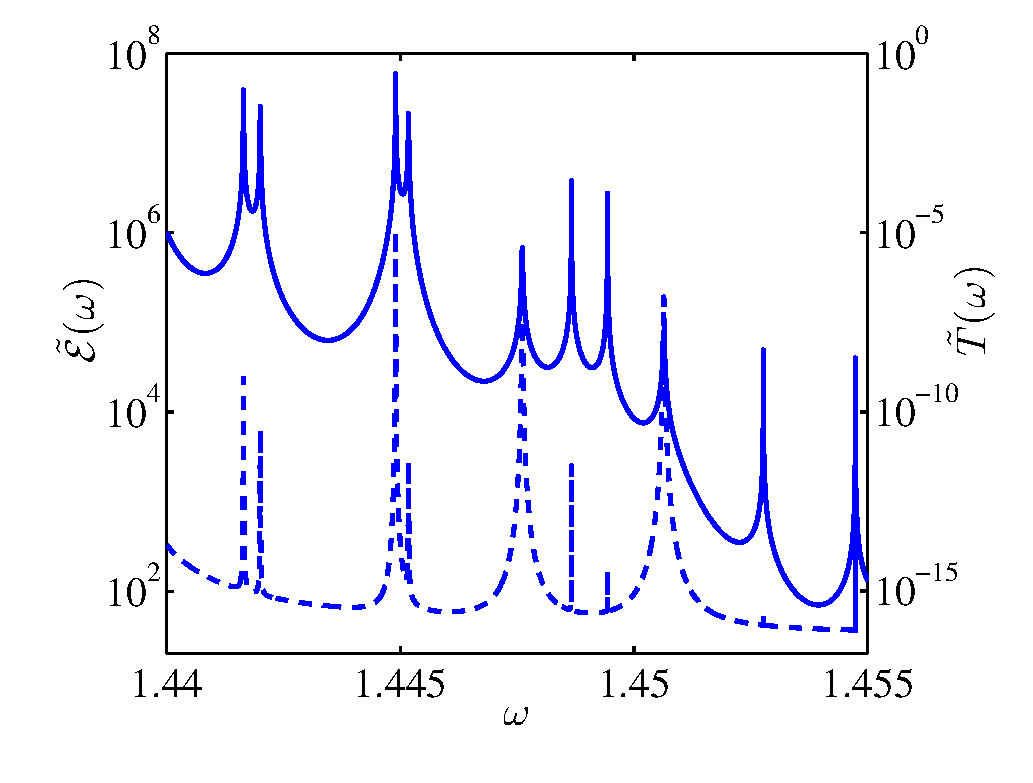
\includegraphics[width=5in]{chapters/Relation_between_transmission_and_energy_stored_in_random_media_with_gain__Phys_Rev_B/pictures/fig2b_tenk_energy_transmission_v_freq}}}
%\begin{flushleft}(a)\end{flushleft}
%\vskip -0.2in
%\scalebox{0.35}{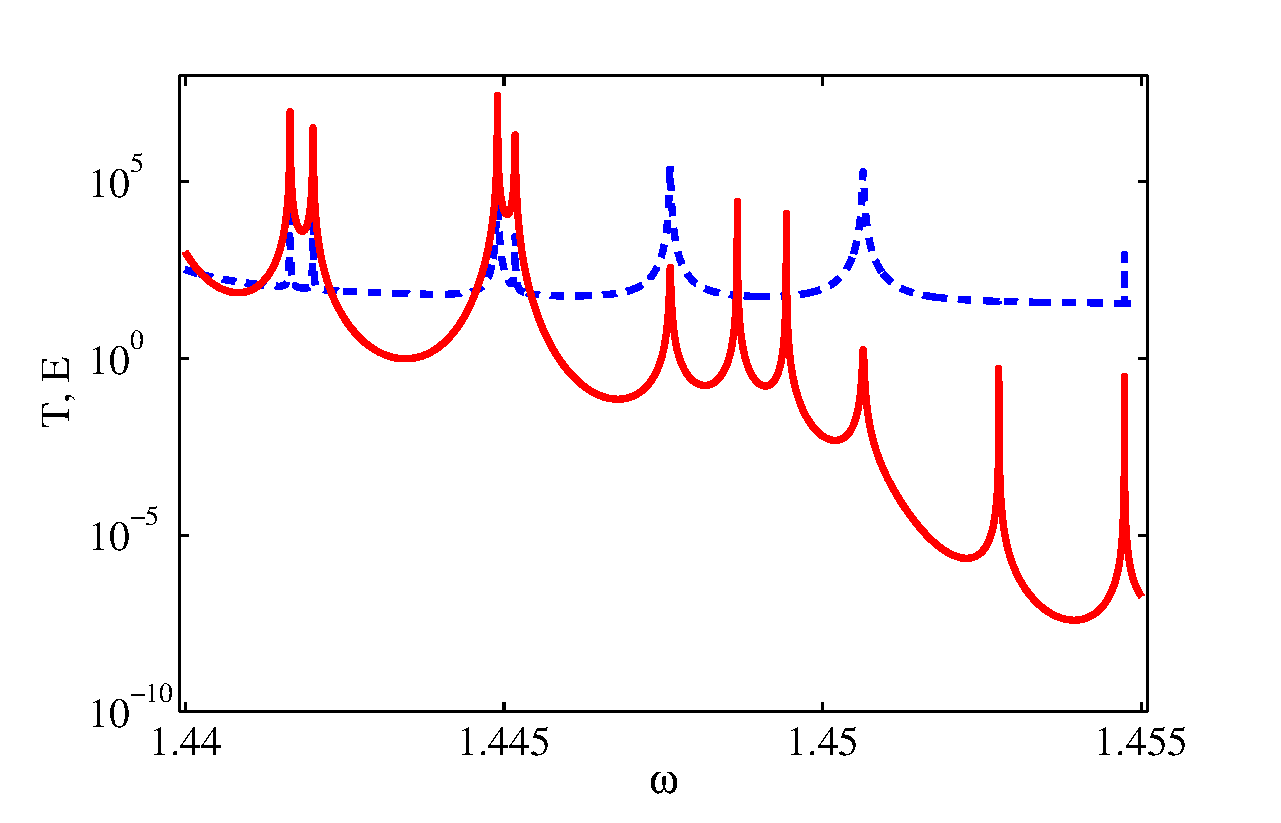
\includegraphics{pictures/tenk_energy_transmission_v_freq}}
%\begin{flushleft}(b)\end{flushleft}
%\vskip -0.1in
%\scalebox{0.38}{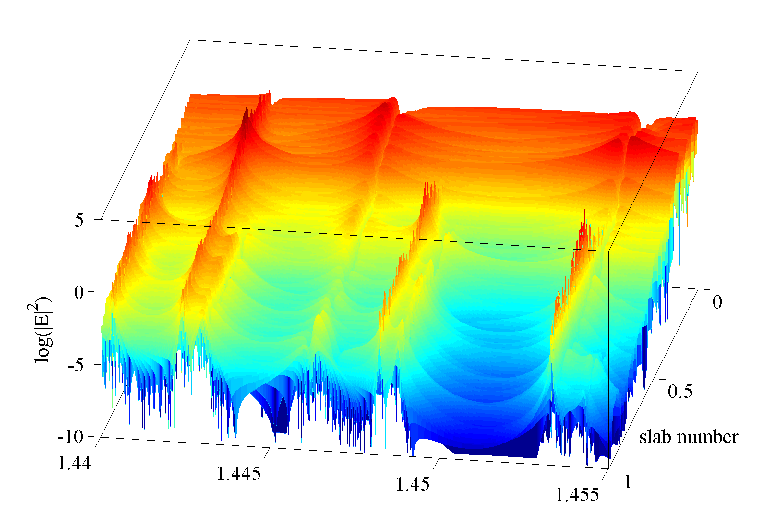
\includegraphics{pictures/electric_field_in_sample}}
\caption[(a) The spatially-resolved electric field in a disordered sample plotted for a range of frequencies.]{
(a) The spatially-resolved electric field in a disordered sample plotted for a range of frequencies. Five clear resonant tunneling states can be identified. 
(b) Transmission (solid line, right $y$-axis) as a function of frequency, $\tilde{T}(\omega)$, is compared to the total energy (dashed line, left $y$-axis) in the sample $\tilde{\cal E}(\omega)$ for one random realization of disorder. No one-to-one correspondence between resonant peak structures is observed.
\label{fig:electricFieldInSample}
}
\end{figure}
%%%%%%%%%%%%%%%%%%%%%%%%%%%%%%%%%%%%%%%

%%%%%%%%%%%%%%%%%%%%%%%%%%%%%%%%%%%%%%%%%%%%%%%%%%%%%%%%%
\subsection{Correlations Between \texorpdfstring{$\tilde{T}$}{T} and \texorpdfstring{$\tilde{\cal E}$}{E}}
\label{sec:correlation_te}
%%%%%%%%%%%%%%%%%%%%%%%%%%%%%%%%%%%%%%%%%%%%%%%%%%%%%%%%%

Motivated by our analysis in Section~\ref{sec:diffusion_general}, we would like to study the dependence of the ratio between transmission and stored energy in the above wave-model. Fig.~(\ref{fig:electricFieldInSample}b) shows $\tilde{T}$ and $\tilde{\cal E}$ as a function of frequency in a single disordered realization. We notice that these two parameters are not closely correlated in the localized regime. Indeed, one can see that unlike the transmission peaks, the peaks in energy are highly dissimilar with some being almost indiscernible. This disparity is an additional source of fluctuation in the ratio  $\tilde{T}/\tilde{\cal E}$. The goal of this section is to understand this behavior.

The field distribution inside the sample gives a clue why the energy may differ from resonance to resonance. At the off-resonant frequencies one observes nearly exponential decay. Whereas at or in the vicinity of a tunneling resonance, two qualitatively distinct behaviors are observed. They are illustrated in Fig.~\ref{fig:Efield_random}.

In the first scenario, c.f.~bold line in Fig.~\ref{fig:Efield_random}, the electric field grows exponentially from the incident boundary towards the localization center $x_0$ and falls off after it. For both segments the characteristic length in the exponential dependencies is set by the localization length. Such behavior is attributed\cite{1983_Azbel_zeroTemp} to the phenomenon of resonant tunneling via a localized state centered at $x_0$. 

In the other case, c.f.~thin line in Fig.~\ref{fig:Efield_random}, an additional negative exponential segment can be identified (notice the change in the direction of incidence, see figure caption). Because this type of behavior leads to significantly less energy stored inside the system, the resonances of this type do not show a pronounced spectral peak in $\tilde{\cal E}$. Although the localized states with spatial profiles as the one shown in bold in Fig.~\ref{fig:Efield_random} were studied in Ref. \cite{1983_Azbel_zeroTemp}, the second scenario exemplified by the thin line in Fig.~\ref{fig:Efield_random} was not described in that or subsequent studies by Azbel and coworkers.

We note that multi-peaked spatial intensity distribution is expected in case of so-called necklace states\cite{1987_Pendry,2005_Wiersma,2006_Genack_1d} when two or more resonant states coexist at (almost) the same energy in the given disorder realization. Such realizations, however, become less probable deep into the localization regime $L\gg\xi$ and  are not directly relevant in the current context. 

We find that, on average, roughly a half of all spectral peaks in transmission do not have the corresponding peak in $\tilde{\cal E}$. As it will become evident from the following discussion, the difference in two types of behavior in Fig.~\ref{fig:Efield_random} originates from the spatial location of the localized state. Indeed, we find that at the frequencies where peaks in transmission and energy occur simultaneously, the center of localization is located close to the incident boundary of the sample. The field distribution is qualitatively similar to the one shown in bold in Fig.~\ref{fig:Efield_random}. In contrast, at the frequencies where the peak in transmission has a significantly less pronounced (or non-distinguishable) peak in energy, the center of localization is located in the second half of the sample (closer to the exit boundary). The field distribution is qualitatively similar to the one depicted with a thin line in Fig.~\ref{fig:Efield_random}.\\

%%%%%%%%%%%%%%%%%%%%%%%%%%%%%%%%%%%%%%%
\begin{figure}
\vskip -.1in
\centerline{\rotatebox{0}{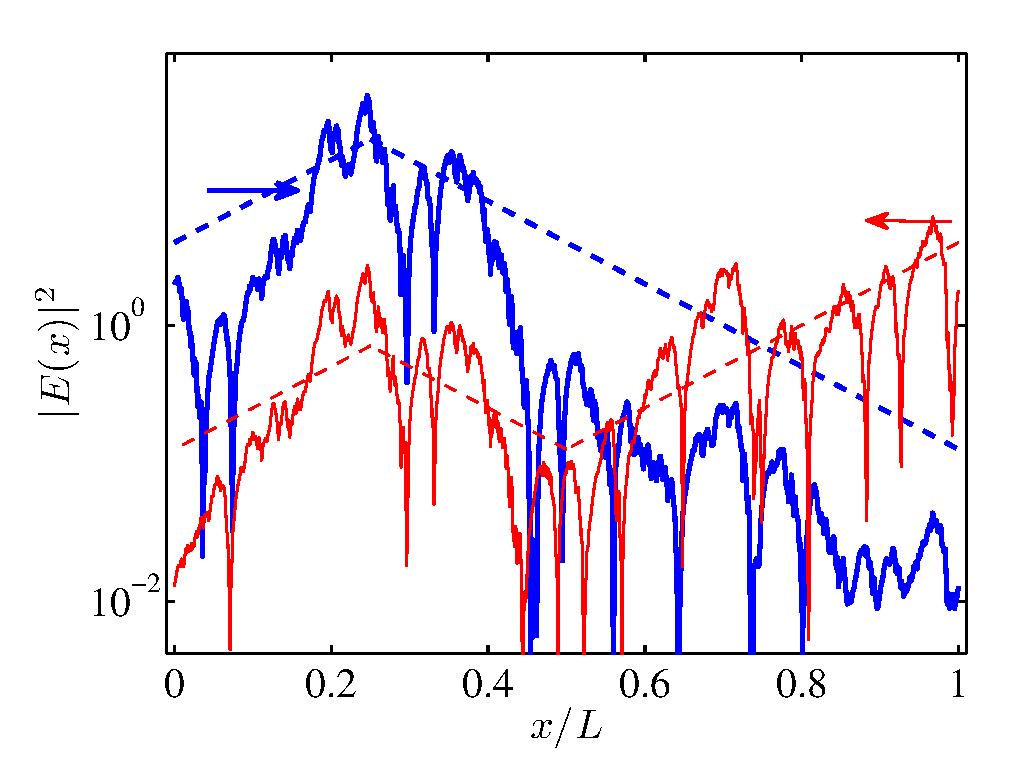
\includegraphics[width=5in]{chapters/Relation_between_transmission_and_energy_stored_in_random_media_with_gain__Phys_Rev_B/pictures/fig3_rlz2_elecfield_14_34}}}
%\scalebox{0.36}{\includegraphics{pictures/rlz2_elecfield_14_34.eps}}
\caption[Two types of the on-resonance electric field distribution inside a passive random medium with the center of localization $x_0$ in the first half (bold lines) and the second half (thin lines) of the sample ($x_0/L \approx 0.25$).]{
Two types of the on-resonance electric field distribution inside a passive random medium with the center of localization $x_0$ in the first half (bold lines) and the second half (thin lines) of the sample ($x_0/L \approx 0.25$). The second case is realized by shining the light onto the same system from the right, which is equivalent to switching boundary conditions from Eq.~(\ref{eq:basis_functions_bc_l}) to Eq.~(\ref{eq:basis_functions_bc_r}). Due to reciprocity, the value of transmission coefficient for both cases is exactly the same. However, the amount of energy stored inside the system is exponentially smaller in the second case. The latter resonance does not show noticeable peak in $\tilde{\cal E}(\omega)$. The dashed lines are the schematic envelope functions formed from segments with $\exp(\pm x/ \xi)$ spatial dependences. The parameters of the system are given in Sec.~\ref{sec:numerical_model}. 
\label{fig:Efield_random}}
\end{figure}
%%%%%%%%%%%%%%%%%%%%%%%%%%%%%%%%%%%%%%%

Realizing that our system is invariant under the time reversal transformation, one is led to the following observation. A sample with a localized state $0<x_0<L/2$ automatically yields the $L/2<x_0<L$ state in the mirror-image sample or, equivalently, by illuminating the same system from the other end as in Fig.~\ref{fig:Efield_random}. The reciprocity of the system makes the transmission coefficient the same in both cases. However, the spatial field distribution inside the system and, thus, energy stored, is dramatically different. In Appx.~\ref{app:qm_model} we show that the effect can be traced to a simple deterministic quantum model and is not specific to random systems. Indeed, the behavior observed in the models described in this section and in Appx.~\ref{app:qm_model} (c.f.~Figs.~\ref{fig:Efield_random},\ref{fig:barrierdefectlog}) can be also obtained in  other models. We checked a periodic stack of dielectric slabs as in Sec.~\ref{sec:numerical_model}, but with no disorder. Electric field distribution for the defect state created by changing the width of a single slab in the stack, appear equivalent to that in Fig.~\ref{fig:barrierdefectlog}.
 
We conclude this section with a summary of our findings: (i) Based on the analytical models we determine that the position of the center of localization ($x_0$) directly affects how much energy is stored in the system. (ii) This variation of stored energy based on the position of the center of localization explains why peaks in energy do not always correspond to the peaks in transmission. (iii) The presence of a peak in energy can be taken as an indication that the center of localization is located close to incident side of the sample. And otherwise, a peak in transmission without its counterpart in energy is indicative t the center of localization lies closer to the exit boundary.

%%%%%%%%%%%%%%%%%%%%%%%%%%%%%%%%%%%%%%%%%%%%%%%%%%%%%%%%%
\subsection{Behavior of \texorpdfstring{$\tilde{T}/\tilde{\cal E}$}{T/E} in Passive Random Medium: Spectral Vicinity of a Resonance}
\label{sec:spectral_te}

%%%%%%%%%%%%%%%%%%%%%%%%%%%%%%%%%%%%%%%%%%%%%%%%%%%%%%%%%

%%%%%%%%%%%%%%%%%%%%%%%%%%%%%%%%%%%%%%%
\begin{figure*}
\vskip -0.0in
\centerline{\rotatebox{0}{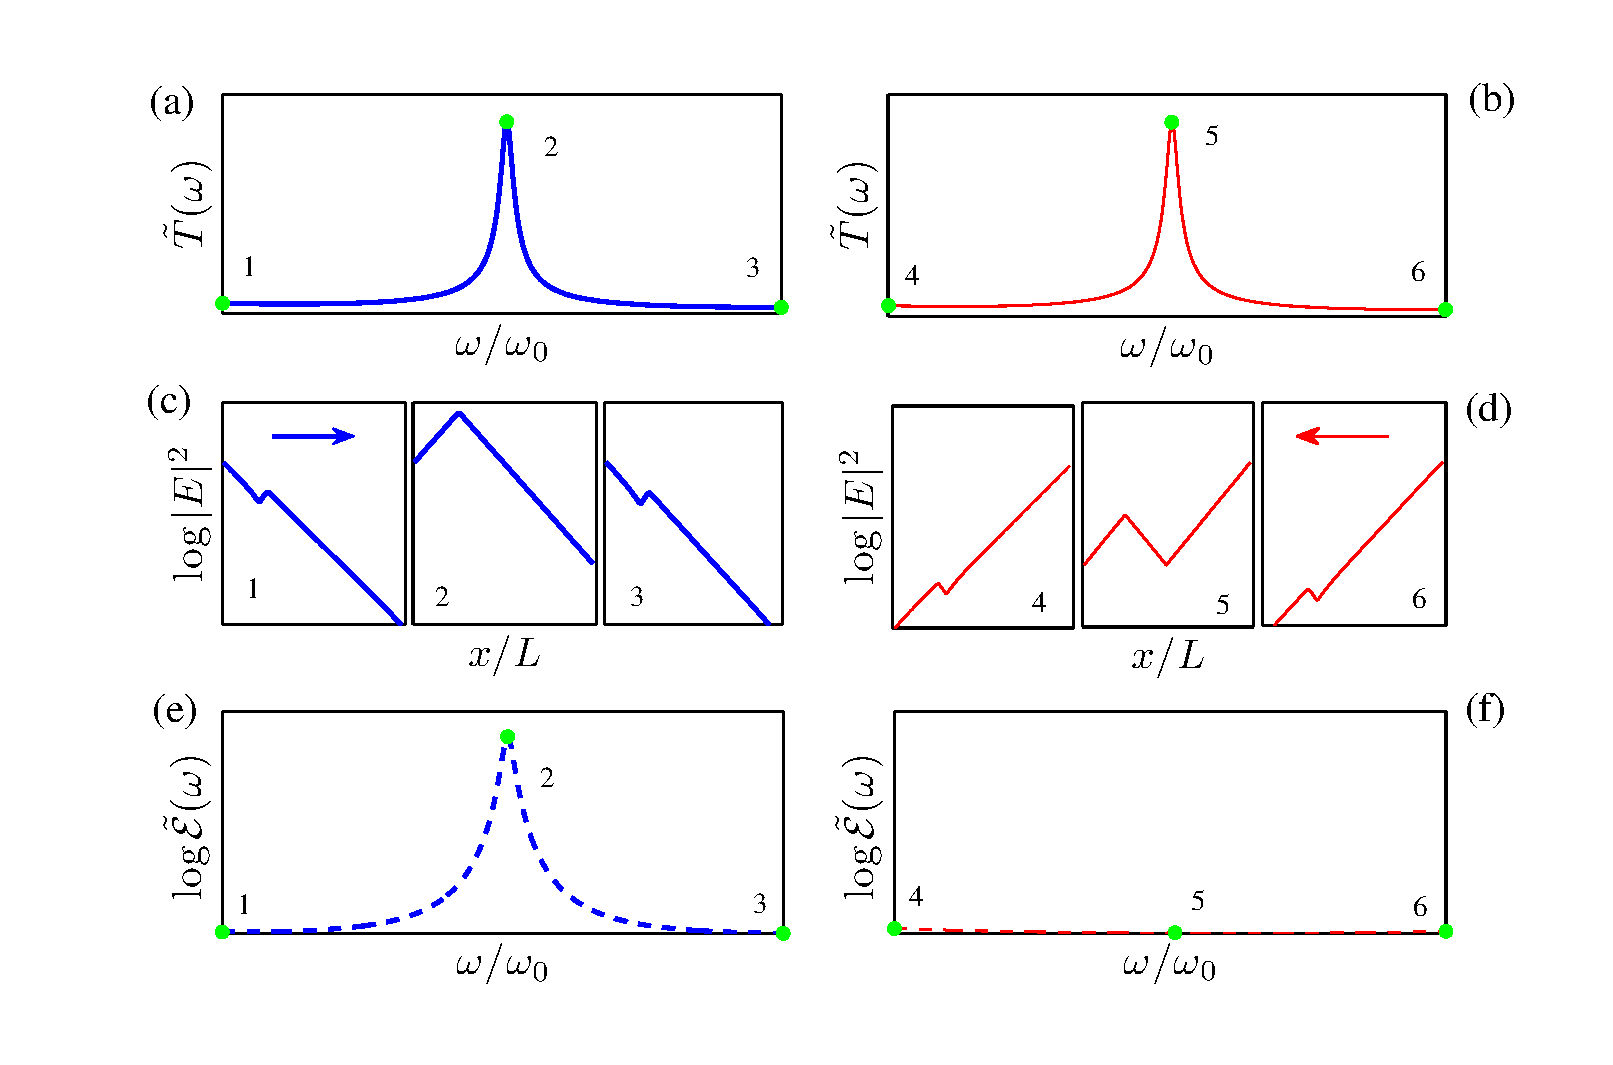
\includegraphics[width=6.75in]{chapters/Relation_between_transmission_and_energy_stored_in_random_media_with_gain__Phys_Rev_B/pictures/fig4_peaks_match_peaks_dont_match}}}
%\centerline{\scalebox{0.65}{\includegraphics{pictures/peaks_match_peaks_dont_match1}}}
\vskip 0.0in
\caption[The dependencies of $\tilde{T}(\omega )$ (a,b); envelope of the electric field  $E(x)$ (c,d); and energy in the system $\tilde{\cal E}(\omega )$ (e,f), are plotted in the spectral vicinity of a transmission resonance associated with a defect in the periodic stack of alternating dielectric layers.]{The dependencies of $\tilde{T}(\omega )$ (a,b); envelope of the electric field  $E(x)$ (c,d); and energy in the system $\tilde{\cal E}(\omega )$ (e,f), are plotted in the spectral vicinity of a transmission resonance associated with a defect in the periodic stack of alternating dielectric layers. The plots (a,c,e) and (b,d,f) are obtained for the defect located at $x_0=L/4$ and $x_0=3L/4$ respectively. In the latter case was realized by changing the direction of illumination to that given by Eq.~(\ref{eq:basis_functions_bc_r}) -- wave incident from the right -- for easy comparison with Figs.~\ref{fig:Efield_random},\ref{fig:barrierdefectlog}. In the first case, the defect center is closer to the incident boundary whereas in the second case it is closer to the exit boundary. Three sets of $E(x)$ in (c,d) are computed at the frequencies marked with dots in (a,b,e,f). The envelopes illustrate the on- and off-resonance field profiles and confirm the applicability of our approximation in Eqs.~(\ref{eq:left},\ref{eq:right},\ref{eq:startingequations},\ref{eq:energy_stored}). For the second case when the defect center is located near the exit boundary, the amount of energy stored inside the medium is dramatically lower. In this case, unlike $\tilde{T}(\omega )$, $\tilde{\cal E}(\omega )$ does not exhibit any noticeable features around $\omega_0$, compare (e) and (f). This effect leads to the asymmetry between $0<x_0<L/2$ and $L/2<x_0<L$ in the $\tilde{T}/\tilde{\cal E}$ as discussed in Sec.~\ref{sec:correlation_te} and Appx.~\ref{app:qm_model}.
\label{fig:peaksmatchnotmatch}}
\end{figure*}
%%%%%%%%%%%%%%%%%%%%%%%%%%%%%%%%%%%%%%%

In this section we employ the knowledge of the spatial profiles of the resonant states gained in Sec.~\ref{sec:correlation_te} and Appx.~\ref{app:qm_model} to obtain a closed analytical expression which qualitatively describes the behavior of $\tilde{T}/\tilde{\cal E}$ in the vicinity of a transmission resonance in terms of relevant system parameters.

In the localization regime, transmission of electromagnetic waves through a random medium occurs via tunneling or, when there exists appreciable spectral overlap with a resonant state inside the sample, via resonant tunneling. Thus, the starting point in our consideration is the simplified expression for frequency-dependent transmission coefficient in the spectral vicinity of a resonance:
\begin{equation}
\tilde{T}(\omega) = \frac{t_0^2}{\left[2(k-k_0)\Delta\right]^2+t_0^2\cosh^2\displaystyle\frac{\left|L-2x_0\right|}{\xi} }
\label{eq:transmission}
\end{equation}
where $k=\omega/c$ and $t_0=\exp(-L/\xi)$ determines the value of the transmission away from the resonance at $k_0$. $\Delta$ is a quantity with the dimensionality of length. It has the physical meaning of the characteristic spatial extent of the region which serves as the resonant ``cavity"\cite{2008_Bliokh}. $\Delta$ is a model dependent quantity which is related to the cavity width in deterministic models, see e.g. \cite{1994_Pendry,2001_Deych_mqw}. In the case of random media, $\Delta$ is the length of the locally transparent region in the sample which serves as a cavity created due to random fluctuation of the disorder. In this system $\Delta$ is comparable to the localization length\cite{2004_Bliokh_wavelet}.

Of course, even within framework of the simplistic model of Appx.~\ref{app:qm_model} the true expression for the transmission coefficient is more complex than Eq.~(\ref{eq:transmission}). However, the latter adequately captures the functional dependence on such parameters as $k-k_0,x_0,\xi$ and ,$L$: Eq.~(\ref{eq:transmission}) follows from the exact solution in the limit $\left|k-k_0\right|\leq\delta k$ and $L\gg\xi$ (which also leads to $\delta k\ll k_0$ condition). Here $\delta k$ is the spectral width of the resonance.

Qualitative analogy between a disordered 1D random medium and a deterministic quantum model similar to that in Appx.~\ref{app:qm_model} was demonstrated in Ref. \cite{2004_Bliokh_wavelet}. Therefore, we expect Eq.~(\ref{eq:transmission}) to be also qualitatively applicable in the random layered medium of Sec.~\ref{sec:numerical_model}.

We note two important properties of Eq.~(\ref{eq:transmission}). First, the maximum (resonant) value of the transmission at $\omega =\omega_0$ is determined by the location of the cavity as $\tilde{T}(\omega_0)=\cosh^{-2}\left(\left|L-2x_0\right|/\xi\right)$. It turns to unity when $x_0=L/2$. Secondly, when the frequency of the incident light is detuned from the resonance $\left|\omega-\omega_0\right|\gg\delta\omega$, the above expression loses it validity -- the presence of the other resonant states must be accounted for.

%%%%%%%%%%%%%%%%%%%%%%%%%%%%%%%%%%%%%%%
\begin{figure}
\centerline{\rotatebox{0}{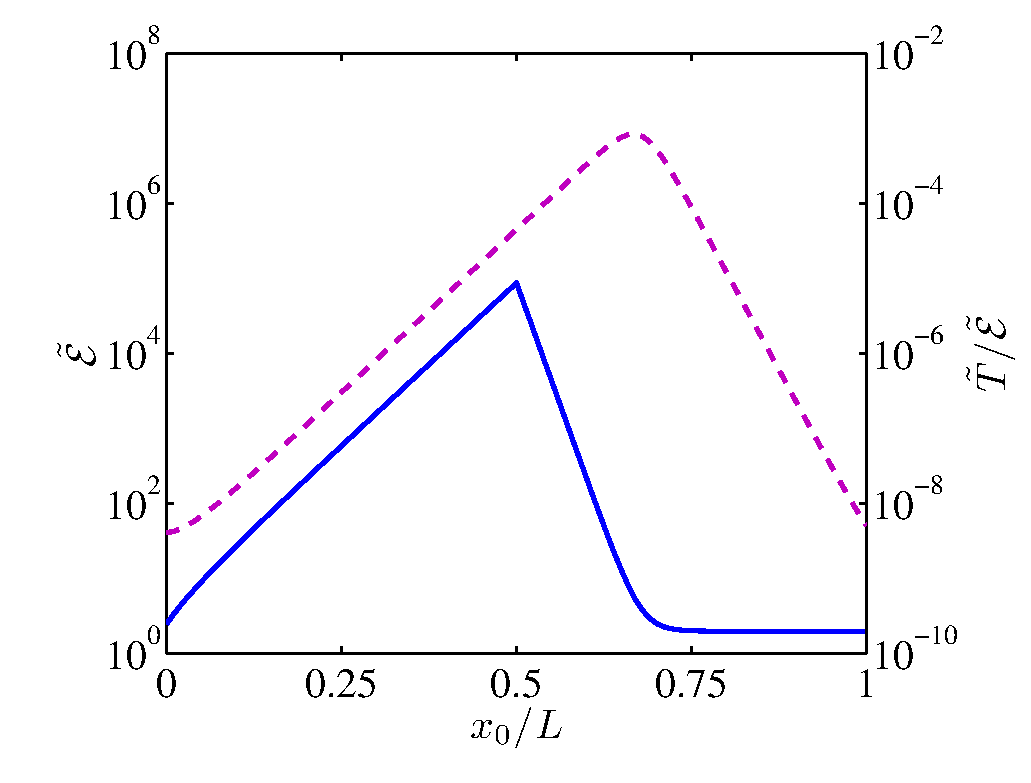
\includegraphics[width=3.5in]{chapters/Relation_between_transmission_and_energy_stored_in_random_media_with_gain__Phys_Rev_B/pictures/fig5_energy_distribution_and_TE_dual_axis}}}
%\vskip -0.0cm
%\centerline{
%\scalebox{0.5}{\includegraphics{pictures/energy_distribution_and_TE_dual_axis.eps}}}
%\vskip -0.0cm
\caption[The solid line plots $\tilde{\cal E}(\omega_0,x_0)$ from Eq.~(\ref{eq:energy_stored}).]{The solid line plots $\tilde{\cal E}(\omega_0,x_0)$ from Eq.~(\ref{eq:energy_stored}). The energy stored inside a random medium falls off sharply (exponentially) when the center of localization $x_0$ increases beyond $L/2$ and reaches the off-resonant value for $x_0>2L/3$. The dashed line with the right $y$-axis represents the ratio between $\tilde{T}(\omega_0,x_0)$ in Eq.~(\ref{eq:transmission}) and  $\tilde{\cal E}(\omega_0,x_0)$ in Eq.~(\ref{eq:energy_stored}). The ratio peaks at the same value of $x_0/L=2/3$. The latter value does not depend on either the localization length $\xi$ or the system length $L$. \label{fig:energydistrib}}
\end{figure}
%%%%%%%%%%%%%%%%%%%%%%%%%%%%%%%%%%%%%%%

%\begin{widetext}
From analysis of random and deterministic models in Sec.~\ref{sec:correlation_te} and Appx.~\ref{app:qm_model}, c.f.~Figs.~\ref{fig:Efield_random},\ref{fig:barrierdefectlog}, we approximate the envelope of the {\it on-resonance} electric field distribution as
\begin{equation}
E(x,\omega_0) = \left\{
\begin{array}{l l}
B(\omega_0,x_0) \exp [ (x-x_0)/\xi ] &\quad 0 < x < x_0 \\
C(\omega_0,x_0) \exp [-(x-x_0)/\xi ] &\quad x_0 < x < L\\
\end{array} \right.
\label{eq:left}
\end{equation}
for $x_0<L/2$; and
\begin{equation}
E(x,\omega_0) = \left\{
\begin{array}{l l}
 A(\omega_0,x_0) \exp [-x      /\xi ] &\quad 0 < x < x_T(\omega_0)   \\
 B(\omega_0,x_0) \exp [ (x-x_0)/\xi ] &\quad x_T(\omega_0) < x < x_0 \\
 C(\omega_0,x_0) \exp [-(x-x_0)/\xi ] &\quad x_0 < x < L \\
\end{array} \right.
\label{eq:right}
\end{equation}
for $x_0>L/2$. Here $A,B,C$ are constants to be determined from the continuity conditions. At the boundaries we set $E(x=0)=1$ and $E(x=L)=\tilde{T}^{1/2}(\omega_0)$. Noticing that $E(x=L,\omega_0)\approx\exp\left[ -|2x_0-L|/\xi\right]$ yields the following expression for the location for the turning point, $x_T(\omega_0)=2x_0-L$, in the case of Eq.~(\ref{eq:right}). In the context of light propagation in random media, such as in Sec.~\ref{sec:numerical_model}, the Eqs.~(\ref{eq:left},\ref{eq:right}) have the meaning of the typical envelope of the true spatial distribution of the electric field in the random systems with the same values of the parameters $(\omega-\omega_0),x_0,\xi$, and $L$.

In both cases above, away from the resonant frequency $k_0$, we see three distinct regions:
\begin{equation}
E(x) = \left\{
\begin{array}{l l}
A(\omega,x_0) \exp[- x     /\xi]  &\quad 0 < x < x_T(\omega)    \\
B(\omega,x_0) \exp[ (x-x_0)/\xi]  &\quad x_T(\omega) < x < x_0  \\
C(\omega,x_0) \exp[-(x-x_0)/\xi]  &\quad x_0 < x < L    \\
\end{array} \right. 
\label{eq:startingequations}
\end{equation}
where $x_T(\omega)$ again has to be determined from the boundary conditions $E(x=0)=1$ and $E(x=L)=T^{1/2}(\omega)$. Fig.~\ref{fig:peaksmatchnotmatch} illustrates the obtained electric field distribution for both $x_0<L/2$ and $x_0>L/2$ cases. It also makes it clear that the energy stored inside the sample varies from resonance to resonance due to the position of the center of localization $x_0$. Indeed, integrating Eqs.~(\ref{eq:left},\ref{eq:right}) gives us the sought expression for $\tilde{\cal E}(\omega)$. At $\omega=\omega_0$ it simplifies to
\begin{equation}
\tilde{\cal E}(x_0)\propto\left\{
\begin{array}{l l}
2\tilde{T}(\omega)\exp\left[2(L-x_0)/\xi\right]-1- \tilde{T}(\omega) & \quad 0  < x_0 < L/2 \\
2\tilde{T}(\omega)\exp\left[2(L-x_0)/\xi\right]+1-3\tilde{T}(\omega) & \quad L/2< x_0 < L   \\
\end{array}
\right.
\label{eq:energy_stored}
\end{equation}
%\end{widetext}
This expression is plotted in Fig.~\ref{fig:energydistrib}. It shows dramatic disparity between the cases $x_0<L/2$ and $x_0>L/2$. Eq.~(\ref{eq:energy_stored}) also shows that even at the frequency of the resonance the amount of energy stored inside the system becomes essentially the same as an off-resonant case for $x_0>2L/3$. The latter value of $x_0$ is independent of any other parameters of the systems such as $\xi$, $L$, etc.

When expressions in Eqs.~(\ref{eq:transmission},\ref{eq:energy_stored}) are combined to form the ratio $\tilde{T}/\tilde{\cal E}$, one obtains highly asymmetric dependence on the position of the center of localization $x_0$, c.f.~Fig.~\ref{fig:energydistrib}. The ratio increases approximately exponentially for $0<x_0<2L/3$ and falls off also exponentially in the interval $2L/3<x_0<L$. This observation confirms our previous conclusion on the sensitivity of the $\tilde{T}/\tilde{\cal E}$ on $x_0$. In the next section we study the effect of (linear) optical amplification on this quantity.

%%%%%%%%%%%%%%%%%%%%%%%%%%%%%%%%%%%%%%%%%%%%%%%%%%%%%%%%%
\subsection{Behavior of \texorpdfstring{$\tilde{T}/\tilde{\cal E}$}{T/E} in Active Random Medium} 
\label{sec:localization_gain}
%%%%%%%%%%%%%%%%%%%%%%%%%%%%%%%%%%%%%%%%%%%%%%%%%%%%%%%%%

%%%%%%%%%%%%%%%%%%%%%%%%%%%%%%%%%%%%%%%%%%%%%%%%%%%%%%%%%%%%%%
\begin{figure}
\centerline{\rotatebox{0}{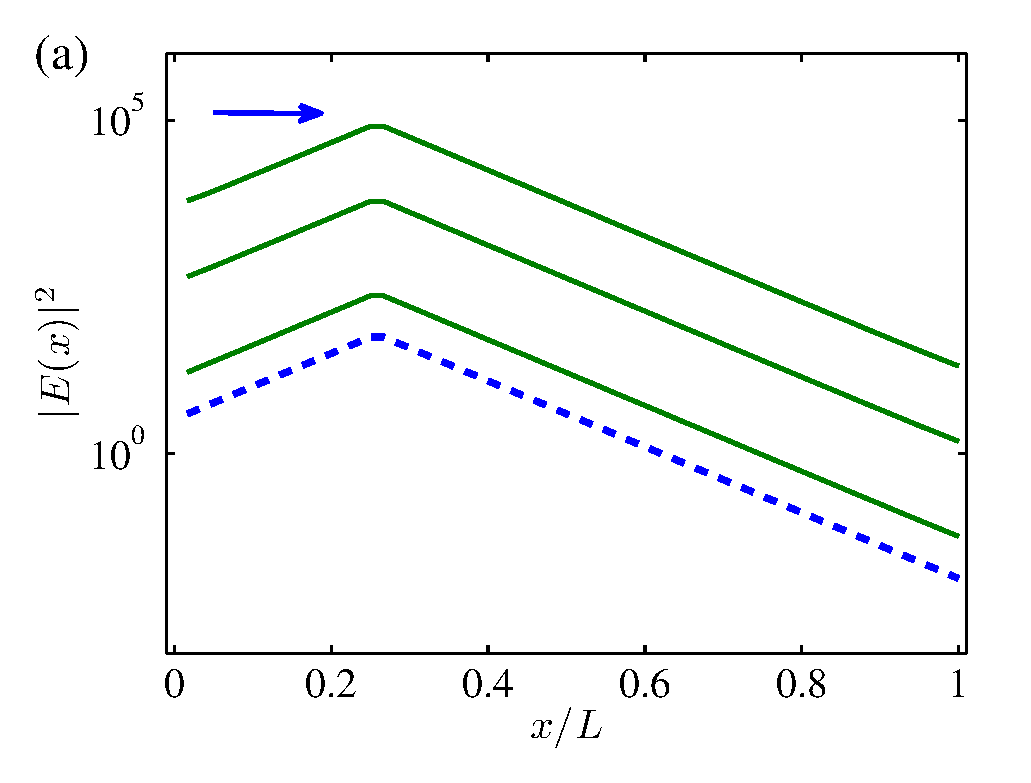
\includegraphics[width=3.25in]{chapters/Relation_between_transmission_and_energy_stored_in_random_media_with_gain__Phys_Rev_B/pictures/fig6a_periodic_34_defect_passive_to_gain2}}}
\centerline{\rotatebox{0}{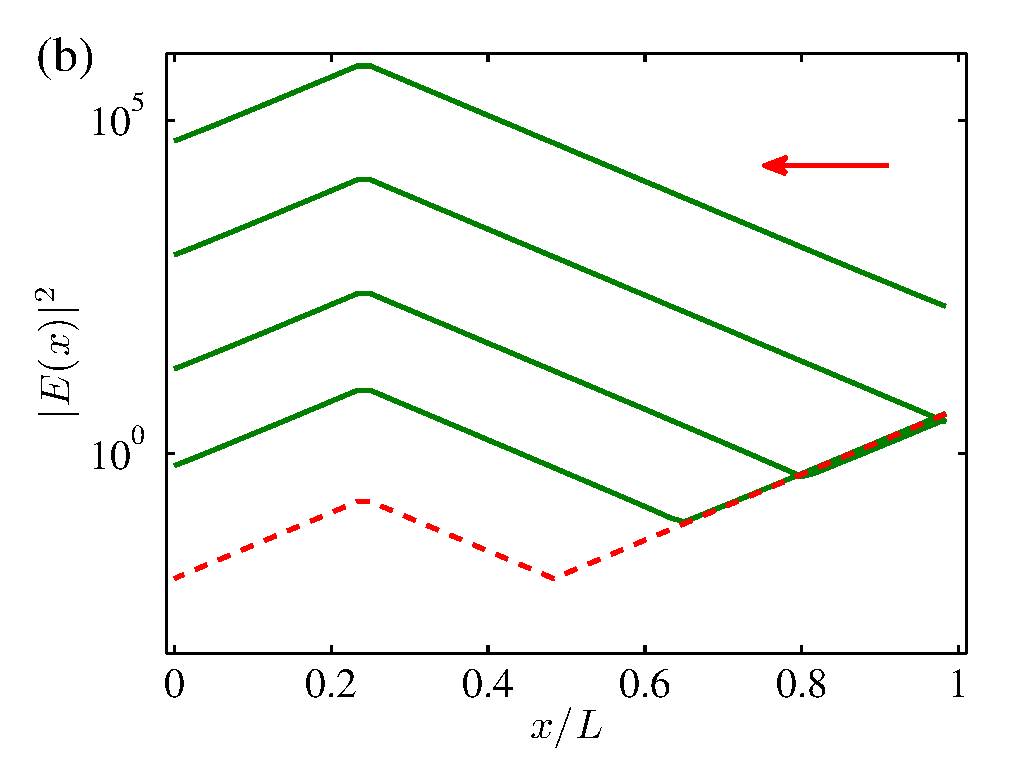
\includegraphics[width=3.25in]{chapters/Relation_between_transmission_and_energy_stored_in_random_media_with_gain__Phys_Rev_B/pictures/fig6b_periodic_14_defect_passive_to_gain2}}}
%\begin{flushleft}
%(a)
%\end{flushleft}
%\vskip -0.7cm
%\centerline{\scalebox{0.35}{\includegraphics{pictures/periodic_34_defect_passive_to_gain2.eps}}}
%\begin{flushleft}
%(b)
%\end{flushleft}
%\vskip -0.7cm
%\centerline{\scalebox{0.35}{\includegraphics{pictures/periodic_14_defect_passive_to_gain2.eps}}}
%\vskip -0.0cm
\caption[An illustration of the effect gain on the electric field distribution in a 1D random medium.]{An illustration of the effect gain on the electric field distribution in a 1D random medium. A periodic stack of alternating dielectric layers with a defect at $x_0=L/4$ is considered. As discussed in Sec.~\ref{sec:correlation_te}, such a model qualitatively describes the field profiles (such as those in Fig.~\ref{fig:Efield_random}) in random media. Panels (a) and (b) show the field envelopes obtained when the system is illuminated (at resonant frequency) from the left and right respectively. Dashed lines correspond to the passive medium. The solid curves (from bottom up) are obtained for $l_{g,cr}/l_g$ equal to $0.5,\ 0.9,\ 0.99$ in (a) and $0.85,\ 0.95,\ 0.98,\ 0.99$ in (b). The field distribution in (b) shows a dramatic modification with an increase of gain.\label{fig:localization_gain}}
\end{figure}
%%%%%%%%%%%%%%%%%%%%%%%%%%%%%%%%%%%%%%%%%%%%%%%%%%%%%%%%%%%%%%

As we observed in Sec.~\ref{sec:diffusion_general}, a change in $T/{\cal E}$ with gain is indicative of a modification of the intensity profile inside a diffusive slab. Similar conclusions can be made in the localized regime. Our simulations demonstrate that a change in $\tilde{T}/\tilde{\cal E}$ indeed signifies the modification of the field distribution inside the random medium. Interestingly, we find that such modifications can be very dramatic in the localization regime. 

To illustrate the effect of linear gain on the spatial profile of the EM field, we employ the deterministic (non-random) model of the periodic stack of alternating dielectric layers with a defect (see Sec.~\ref{sec:spectral_te}). The gain is simulated by adding a spatially constant imaginary part to the dielectric constant of the medium  as $\epsilon(x)\rightarrow\epsilon(x)+i\alpha$. As previously discussed in Sec.~\ref{sec:intro}, such modeling of stimulated amplification is justified for values of gain up to the threshold for random lasing.

The results of our simulations are plotted on Fig.~\ref{fig:localization_gain}. One can see the strong enhancement of the electric field in the vicinity of the center of localization for the defect located in the farther half of the sample. Such enhancement is accompanied by the shift of the turnaround point $x_T$, where the negative exponential crosses over to the positive exponential behavior, towards the sample boundary. At a certain value of the gain parameter, the negative exponential segment of the $E(x)$ disappears and the field profile assumes the limiting shape which coincides with that under excitation from the opposite boundary of the system. The above observations also hold in the random medium model of Sec.~\ref{sec:correlation_te}. 

At first glance, the modification of the field profile due to gain seems to disagree with the conclusions in Refs.~\cite{2002_Jiang_Loc_Modes_Lasing,2002_Sebbah_Vanneste,2005_Vanneste} where (in localized regime) little or no change in the field pattern was found with an increase of amplification. The apparent discrepancy can be explained if one compares the methods used to excite the system. In our work, we consider the transmission experiment setup, whereas in the previous works \cite{2002_Jiang_Loc_Modes_Lasing,2002_Sebbah_Vanneste,2005_Vanneste} the system is excited throughout its entire volume or relatively close to the center of localization. Under such excitation conditions, the situation shown in Fig.~\ref{fig:localization_gain}a is always realized \cite{2010_Payne_loc_criterion}. We also note that the mode distribution in Fig.~\ref{fig:localization_gain}b is observed to converge to that in Fig.~\ref{fig:localization_gain}a when the gain approaches its critical value. Then the field distribution is maintained by the gain with little reliance on the incident energy.

%%%%%%%%%%%%%%%%%%%%%%%%%%%%%%%%%%%%%%%%%%%%%%%%%%%%%%%%%
%\subsection{Gain-induced electric field modifications\label{sec:localization_gain_explained}} 
%%%%%%%%%%%%%%%%%%%%%%%%%%%%%%%%%%%%%%%%%%%%%%%%%%%%%%%%%

%%%%%%%%%%%%%%%%%%%%%%%%%%%%%%%%%%%%%%%%%%%%%%%%%%%%%%%%%%%%%%
\begin{figure*}
%\vskip -0.0cm
\centerline{\rotatebox{0}{
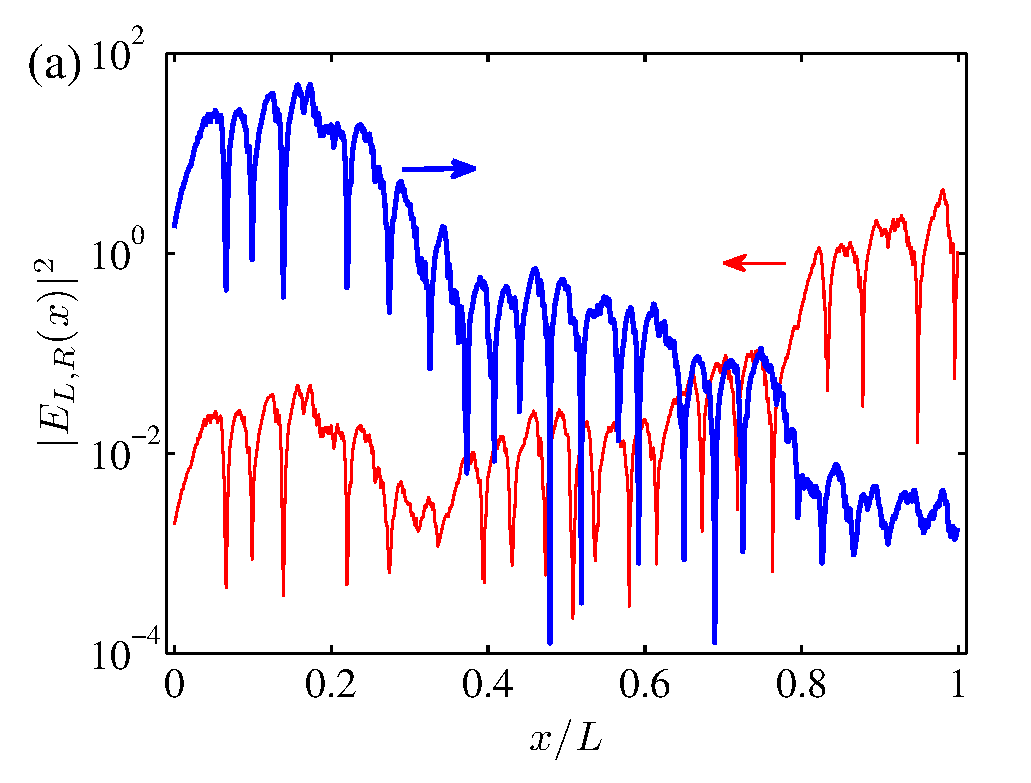
\includegraphics[width=2in]{chapters/Relation_between_transmission_and_energy_stored_in_random_media_with_gain__Phys_Rev_B/pictures/fig7a_alpha_beta_electric_field}
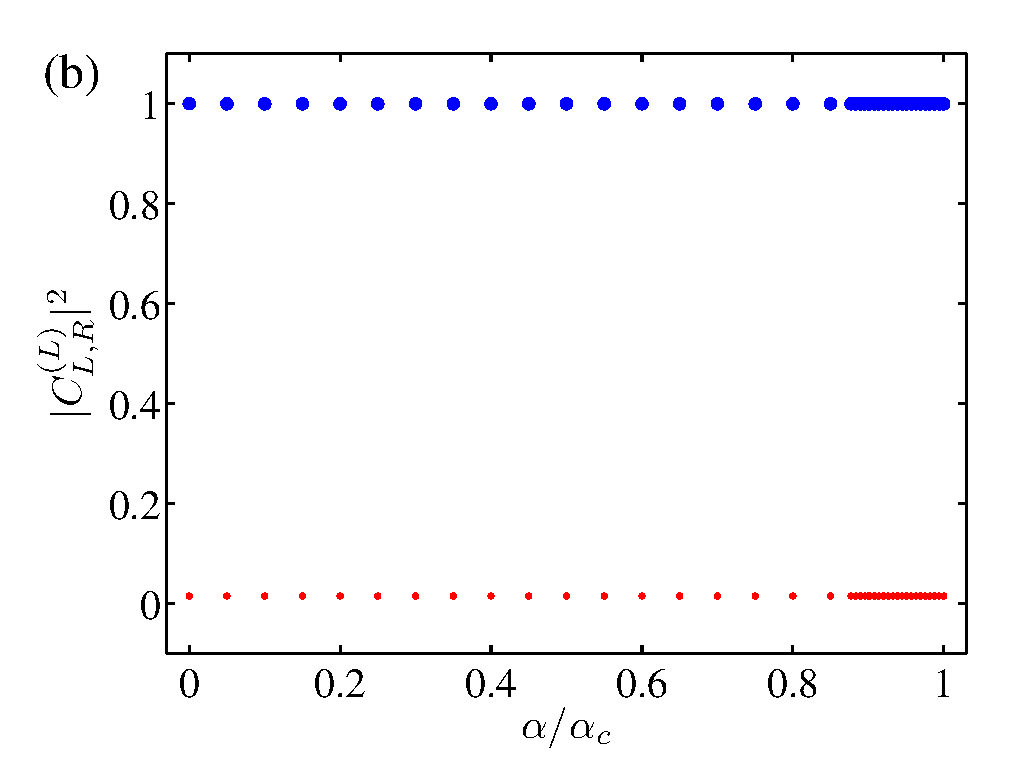
\includegraphics[width=2in]{chapters/Relation_between_transmission_and_energy_stored_in_random_media_with_gain__Phys_Rev_B/pictures/fig7b_alpha2_beta2}
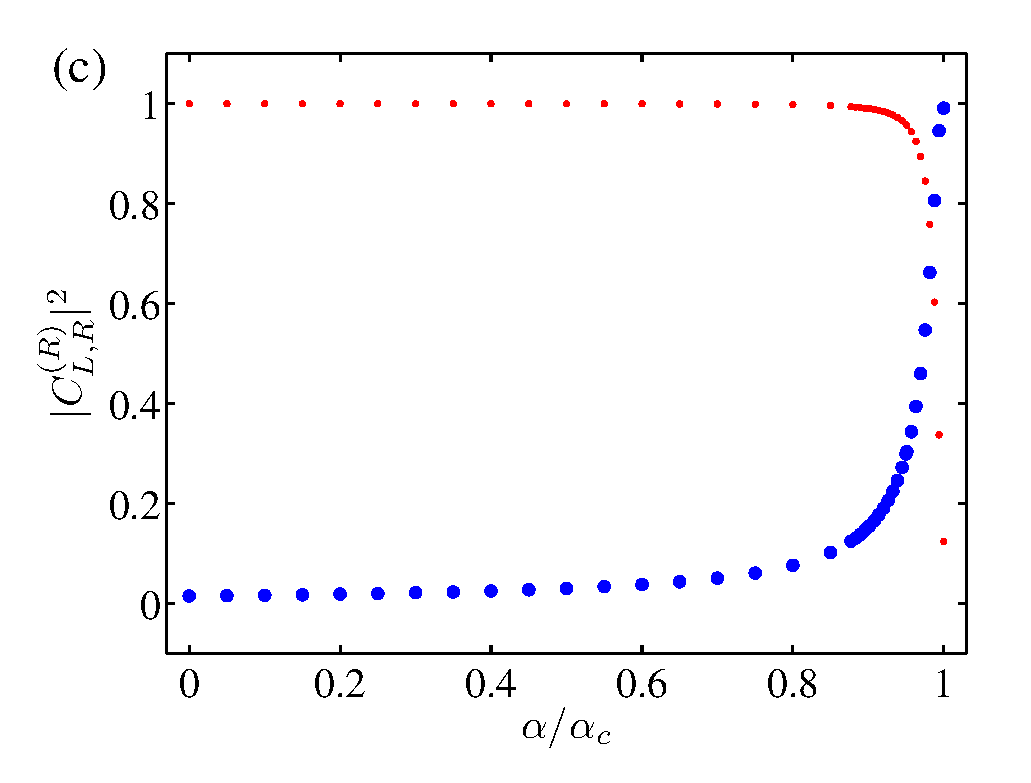
\includegraphics[width=2in]{chapters/Relation_between_transmission_and_energy_stored_in_random_media_with_gain__Phys_Rev_B/pictures/fig7c_alpha1_beta1}
}}
%\centerline{
%\scalebox{0.33}{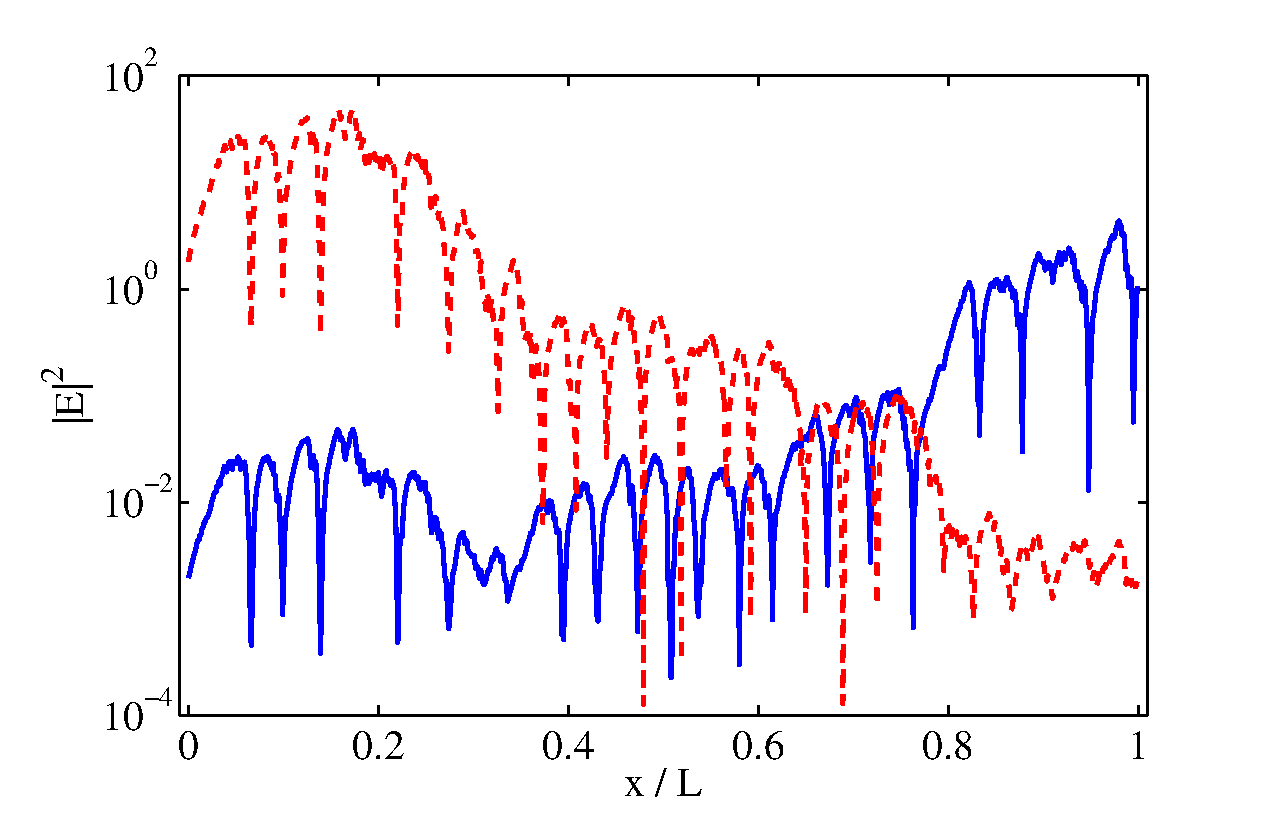
\includegraphics{pictures/alpha_beta_electric_field}}
%\scalebox{0.33}{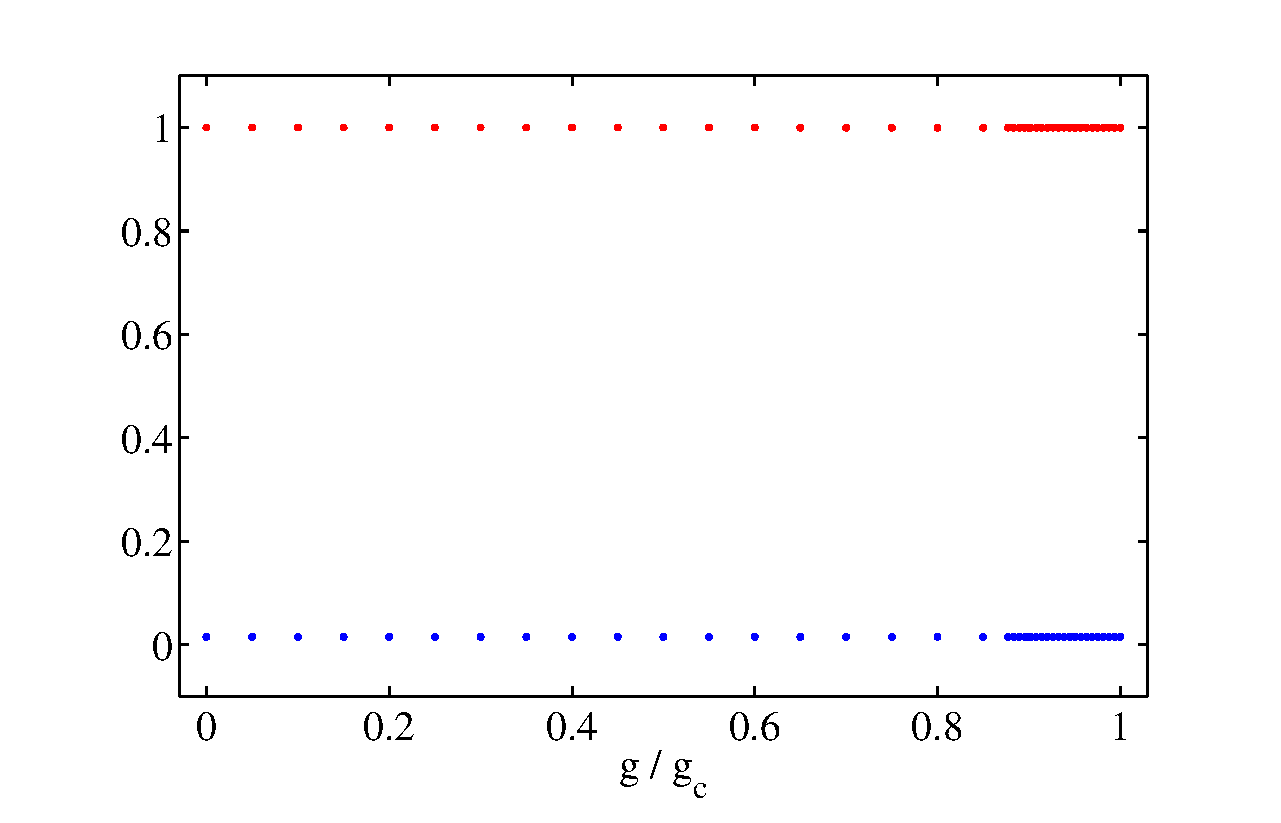
\includegraphics{pictures/alpha2_beta2}}
%\scalebox{0.33}{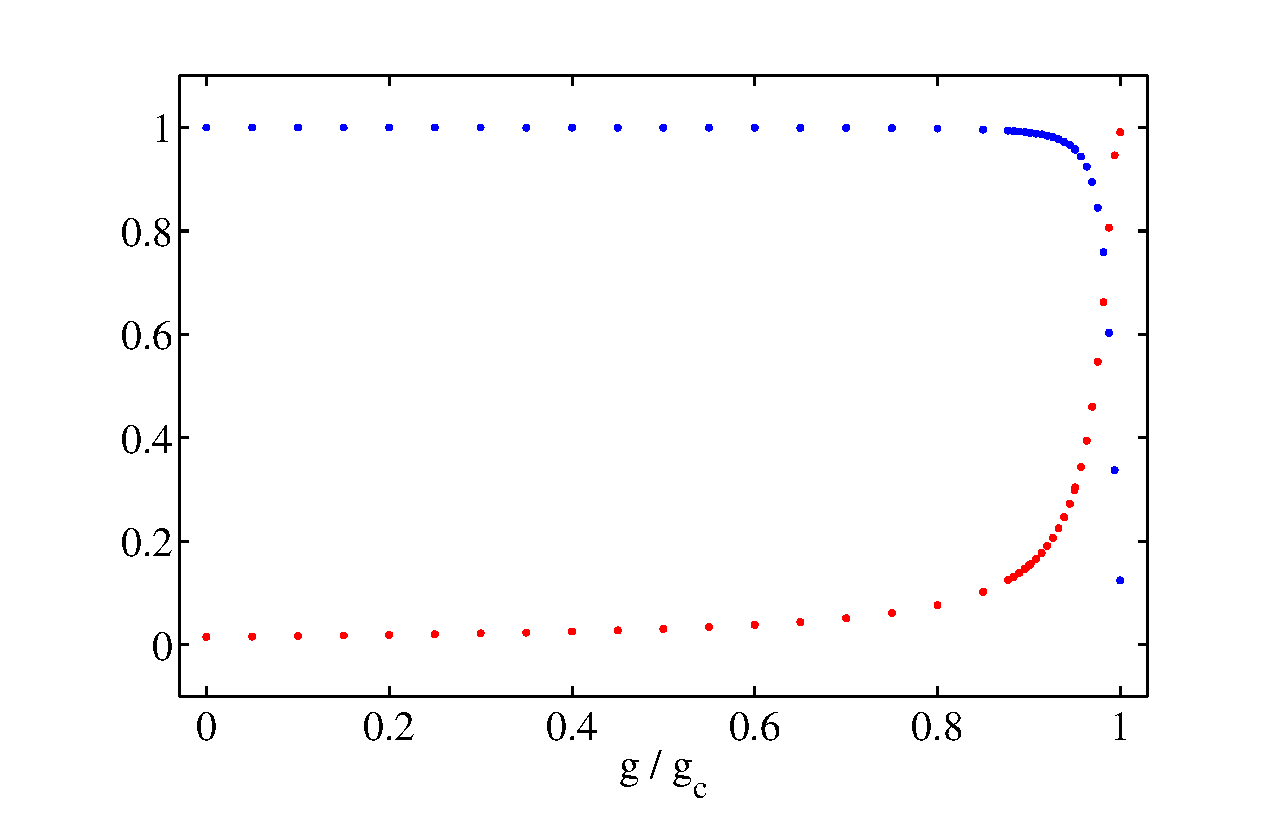
\includegraphics{pictures/alpha1_beta1}}}
%\vskip -0.0cm
\caption[Panel (a) plots $E_{L,R}(x,\omega_c)\equiv  E^{(L,R)}(x,\omega_c,\alpha=0)$ defined by the boundary conditions in Eqs.~(\ref{eq:basis_functions_bc_l},\ref{eq:basis_functions_bc_r}), see text for notations.]{Panel (a) plots $E_{L,R}(x,\omega_c)\equiv  E^{(L,R)}(x,\omega_c,\alpha=0)$ defined by the boundary conditions in Eqs.~(\ref{eq:basis_functions_bc_l},\ref{eq:basis_functions_bc_r}), see text for notations. For non-zero gain, $\alpha>0$, the electric field distributions $E^{(L,R)}(x,\omega_c,\alpha)$ are found to be qualitatively similar to those in Fig.~\ref{fig:localization_gain}. We decompose them in terms of the functions shown in (a), and the resulting coefficients $C_{L,R}^{(L)}(\alpha)$ and $C_{L,R}^{(R)}(\alpha)$, defined in Eq.~(\ref{eq:C_completeness}), are plotted in (b) and (c) respectively. We find that the close resemblance between $E_{L}(x,\omega_c)$ and $E^{(c)}(x,\omega_c)$ (the solution in the closed system) makes it the dominant limiting profile in the vicinity of threshold for random lasing, regardless of the direction of excitation. In all three panels, thick / thin curve and large / small symbols refer to  $E_{L}(x,\omega_c)$ / $E_{R}(x,\omega_c)$.\label{fig:alphabeta}}
\end{figure*}
%%%%%%%%%%%%%%%%%%%%%%%%%%%%%%%%%%%%%%%%%%%%%%%%%%%%%%%%%%%%%%

Below we provide a simple physical picture for the modification of the electric field with an increase of optical gain. 

We start by considering the passive system. We recall that our sample is an open system where a wave is incident onto the system and one observes the scattered (reflected and transmitted) signals.  Under these conditions a continuous wave (CW) solution of the Maxwell equations with the given frequency is a complex function. The complex conjugate of such a solution is also a (linearly independent) solution for the same frequency. In general, any two (because Maxwell's equation is the second order differential equation) linearly independent solutions can be used as a basis for expressing any other solution at the same frequency $\omega$. 

Now we would like to consider two particularly important solutions of the Maxwell equation in the random 1D sample with the boundary conditions defined by Eqs.~(\ref{eq:basis_functions_bc_l},\ref{eq:basis_functions_bc_r}). They correspond to the left- and right-incident cases respectively as considered in Sec.~\ref{sec:correlation_te} and Appx.~\ref{app:qm_model} with $r_{L,R}(\omega),t_{L,R}(\omega)$ being the corresponding amplitude reflection and transmission coefficients. To check the linear independence of these two solutions it suffices to verify that their Wronskian (it is independent of $x$ in our model of disorder $\epsilon(x)$) is non-zero for one particular value of $x$. At $x=0$ the Wronskian can be computed from the boundary conditions  Eqs.~(\ref{eq:basis_functions_bc_l},\ref{eq:basis_functions_bc_r}) as $-2it_R(\omega)\omega/c\neq 0$.

At some special frequencies $\omega_c$, a linear combination  $E^{(c)}(x,\omega_c)=C_L^{(c)} E_{L}(x,\omega_c)+C_R^{(c)} E_{R}(x,\omega_c)$ can be formed such that conditions $E^{(c)}(x=0,\omega_c)=0$ and $E^{(c)}(x=L,\omega_c)=0$ are satisfied simultaneously. Such $\omega_c$'s  correspond to the true eigen-modes of the closed system -- the system defined by $\epsilon(0\leq x\leq L)$ with zero (reflecting) boundary conditions at $x=0,L$. We numerically obtained such solutions in our 1D random model and found that the single cusp solution (similar to $E_{L}(x,\omega_c)$ depicted with thick lines in Figs. (\ref{fig:Efield_random},\ref{fig:barrierdefectlog})) makes the dominant contribution to $E^{(c)}(x,\omega_c)$. This may explain why the other profile with the negative exponential tunneling segment (similar to $E_{R}(x,\omega_c)$ depicted with thin lines in Figs. (\ref{fig:Efield_random},\ref{fig:barrierdefectlog})) is not seen under uniform excitation as in Refs.~\cite{2002_Jiang_Loc_Modes_Lasing,2002_Sebbah_Vanneste,2005_Vanneste}.

We now turn to the case of random medium with gain, $\alpha>0$, and consider the spatial field distribution obtained when system is illuminated from the left, $E^{(L)}(x,\omega_c,\alpha)$, and from the right $E^{(R)}(x,\omega_c,\alpha)$, c.f.~Fig.~\ref{fig:localization_gain}. In this case, the distributions can no longer, strictly speaking, be expressed in terms of $E_{L,R}(x,\omega_c)\equiv  E^{(L,R)}(x,\omega_c,\alpha=0)$. However, in the regime of localized transport considered here, $\alpha<\alpha_{cr}\ll\omega_c$, the deviation from completeness of the basis $E_{L,R}(x,\omega_c)$ are to remain small so that  the dependence of $E(x,\omega_c,\alpha)$ on gain can be still reliably approximated by $\alpha$-dependent $C_{L}(\alpha)$,$C_{R}(\alpha)$:
\begin{equation}
E(x,\omega_c,\alpha)\simeq C_L(\alpha) E_{L}(x,\omega_c)+C_R(\alpha) E_{R}(x,\omega_c).
\label{eq:C_decomposition}
\end{equation}
The applicability of the approximation in Eq.~(\ref{eq:C_decomposition}) is verified numerically by computing  
\begin{equation}
C_{L,R}^{(L,R)}(\alpha)=\int_{0}^{L} E^{(L,R)}(x,\omega_c,\alpha)E_{L,R}^*(x,\omega_c)dx.
\label{eq:C_completeness}
\end{equation}
Figs.~\ref{fig:alphabeta}b,c show $C_{L,R}^{(L)}(\alpha)$ and $C_{L,R}^{(R)}(\alpha)$ respectively. Here we select a random realization with a localization center at $x_0\sim L/4$ where passive profiles, depicted in Fig.~\ref{fig:alphabeta}a, show the two characteristic shapes considered in Figs.~\ref{fig:Efield_random},\ref{fig:barrierdefectlog},\ref{fig:localization_gain}. When gain is added to the system, we observe that $E^{(L)}(x,\omega_c,\alpha)\propto E_{L}(x,\omega_c)$ for all values of gain, c.f.~Fig.~\ref{fig:alphabeta}b. In contrast, $E^{(R)}(x,\omega_c,\alpha)$ exhibited a crossover behavior from $E^{(R)}(x,\omega_c,\alpha)\propto E_{R}(x,\omega_c)$ for small $\alpha$, to $E^{(R)}(x,\omega_c,\alpha)\propto E_{L}(x,\omega_c)$ in the vicinity of lasing threshold. This result corroborates the findings of the previous Sec.~\ref{sec:localization_gain}, c.f.~Fig.~\ref{fig:localization_gain}, that the modification of the electric field distribution with an increase of amplification strength is possible in the localized regime. Here we have shown that it occurs due to the existence of two possible mode profiles (at the same frequency), of which only one strongly resembles the solution of the system with closed-boundaries. It is the function with no turning point which defines the lasing mode in the vicinity the threshold for random lasing. 

Finally, we note that the solutions $E_{L,R}(x,\omega)$ should not be confused with the quasi-mode $E(x,\omega_c+i\varepsilon)$ of the system with the outgoing boundary conditions obtained at the complex frequency $\omega_c+i\varepsilon$ where e.g. transmission becomes singular. Such quasi-modes are often invoked in discussion of modes involved in random lasing. However, for a uniform gain in the form $\epsilon(x)(1+i\alpha)$ the dominant mode profile $E^{(L)}(x,\omega_c,\alpha_{cr})$ does indeed coincide with the quasi-mode due to equivalence between $\epsilon(x)(1+i\alpha)\omega_c/c$ and $\epsilon(x)(\omega_c+i\varepsilon)/c$.

%%%%%%%%%%%%%%%%%%%%%%%%%%%%%%%%%%%%%%%%%%%%%%%%%%%%%%%%%
\section{DISCUSSION AND OUTLOOK}
\label{sec:discussion_TE}
%%%%%%%%%%%%%%%%%%%%%%%%%%%%%%%%%%%%%%%%%%%%%%%%%%%%%%%%%

In this work we have studied the relationship between transmission of light through passive and active random media and the amount of the electromagnetic energy stored in it. The ratio of these two quantities does not show a tendency to diverge with an increase of the gain strength and, thus, is a good candidate for a parameter which can quantify the enhancement of the mesoscopic phenomena  random medium with amplification \cite{2004_Yamilov_intensity,2005_Yamilov_correlations,2006_Yamilov_conductance}. 

In Sec.~\ref{sec:diffusion_section} we established a connection between the ratio of the ensemble-averaged quantities $T/{\cal E}$ and the spatially dependent diffusion coefficient, Eq.~(\ref{eq:TE_vs_D}), in a passive random medium. This relation implies that a deviation (decrease) of $T/{\cal E}$ from the value given by that expression with the classical un-renormalized diffusion coefficient $D(z)\equiv D_0=c\ell/3$ may be attributed to the localization effects. 

In Sec.~\ref{sec:diffusion_general} we obtained the expressions for $T$ and ${\cal E}$ in the diffusive random medium with amplification. Drawing an analogy with the passive systems, we conjecture that the decrease in $T/{\cal E}$ below the level established by Eq.~(\ref{eq:TE_analytical}) may be interpreted as a manifestation of an enhancement of mesoscopic correction in transport in systems with gain. We plan to examine the validity of this conjecture in future work.

We argue that in random media with strong sample-to-sample fluctuations, such as systems with large gain or strongly scattering media, the ratio between $\tilde{T}$ and $\tilde{\cal E}$ from the same disorder realization needs to be formed before performing statistical averages. This led us to investigate the relationship between these two parameters in systems in the localized regime, c.f.~Sec.~\ref{sec:localization_passive}. Although the ratio $\tilde{T}/\tilde{\cal E}$ does not tend to diverge when gain is added, it exhibits additional fluctuations due to the sample orientation (or, equivalently, the direction of the incident wave) even in the passive system, c.f.~Sec.~\ref{sec:correlation_te}. In Sec.~\ref{sec:spectral_te},\ref{app:qm_model} we attribute the fluctuations to the dependence on the position of the localization center inside the system. This is unlike the transmission $\tilde{T}$, which is independent of direction of illumination (because of reciprocity) -- it is the same for both field distributions depicted in Fig.~\ref{fig:Efield_random}. One possibility to generalize the transmission in the active random media, while retaining the desired cancellation  of the divergence in the vicinity of the threshold for random lasing, is to consider the modified parameter similar to the one studied in this work: $\tilde{T}_G(\alpha)=\left(\tilde{T}(\alpha)/\tilde{\cal E}(\alpha)\right)\times\tilde{\cal E}_0$. Here $\tilde{\cal E}_0\equiv\tilde{\cal E}(\alpha=0)$ is the energy stored in the random medium with no gain. All quantities entering the expression for $\tilde{T}_G$ should be evaluated for each disorder realization prior to any statistical analysis. By construction, $\tilde{T}_G(\alpha)$ reduces to the transmission in a 1D system without gain ($\alpha\rightarrow 0$) and can be generalized in the higher dimensional systems as the (average) dimensionless conductance upon statistical averaging. Hence, one can refer to $T_G$ as generalized transmission (conductance).

In future, we plan to investigate both theoretically and experimentally the statistical properties of both $\tilde{T}(\alpha)/\tilde{{\cal E}}(\alpha)$ and $T_G(\alpha)$ in random medium with gain. Experimentally, all quantities entering their definition can be determined from near-field scanning measurements in two-dimensional random media -- structurally disordered semiconductor films. This opens up a possibility to corroborate and extend the results of this study. 

%%%%%%%%%%%%%%%%%%%%%%%%%%%%%%%%%%%%%%%%%%%%%%%%%%%%%%%%%
\section{ACKNOWLEDGMENTS}
%%%%%%%%%%%%%%%%%%%%%%%%%%%%%%%%%%%%%%%%%%%%%%%%%%%%%%%%%
 
This work was supported by National Science Foundation Grant Nos. DMR-0704981 and DMR-0808937. The numerical
results obtained at the Tera-Grid, Grants No. DMR-090132 and No. DMR-100030. AY is grateful to S. Skipetrov, A. Lagendijk and B. van Tiggelen for valuable comments.

\section{APPENDIX}
%\appendix

\subsection{Derivation of Equation~(\ref{eq:TE_vs_D})}
\label{app:Dz_derivation}
We consider a slab geometry, where we explicitly  separate the coordinate $z$ normal to the slab from the perpendicular component ${\bf \rho}$ as ${\bf r}=({\bf \rho},z)$. Assuming no dependence on ${\bf \rho}$ allows us to rewrite Eq.~(\ref{eq:Jflux}) in the form
\begin{equation}
\langle J_z(z)\rangle=
\displaystyle -D(z)\frac{d\langle {\cal W}(z)\rangle}{dz}.
\label{eq:Jfluxz}
\end{equation}
Independence of ${\bf \rho}$ is insured for the plane-wave illumination boundary condition which we assume here. 

In the CW regime when the energy density ${\cal W}(z)$ is stationary, $\partial \langle {\cal W}(z)\rangle/\partial t=0$, it follows from Eq.~(\ref{eq:Jflux_conserv}) that the $z$-component of flux is constant for $z>z_p\sim\ell$. The value of the constant can be obtained from the boundary condition at $z=L$ as
\begin{equation}
\langle J_z(z)\rangle=\left\{
\begin{array}{l l}
\langle J_z(L)\rangle\equiv J_0 T,&\quad z_p<z<L\\
\langle J_z(0)\rangle\equiv -J_0 R,&\quad 0<z<z_p\\
\end{array} \right.
\label{eq:Jfluxz_const}
\end{equation}
where $T$ is the transmission coefficient. Furthermore, by integrating Eq.~(\ref{eq:Jflux_conserv}) over the entire system we obtain the flux conservation $\langle J_z(L)\rangle -\langle J_z(0)\rangle =J_0 T-(-J_0 R)=J_0(T+R)=J_0$.

After establishing Eq.~(\ref{eq:Jfluxz_const}), we can return to finding the energy stored inside the system from Eq.~(\ref{eq:Jfluxz}). An integration over $z$ gives
\begin{equation}
\displaystyle\int_z^L\frac{\langle J_z(z^\prime)\rangle dz^\prime}{D(z^\prime)}=-\langle {\cal W}(L)\rangle + \langle {\cal W}(z)\rangle.
\label{eq:E1}
\end{equation}
The energy density $\langle {\cal W}(L)\rangle$ at the right boundary can be expressed in terms of right- and left-propagating fluxes $\langle J_+(L)\rangle=J_0T$, $\langle J_-(L)\rangle=0$ using Eqs.~(\ref{eq:diffusive_flux}). We obtain $\langle {\cal W}(L)\rangle=2J_0T/c$. To take advantage of the fact that $\langle J_z(z)\rangle$ is piecewise constant, c.f.~Eq.~(\ref{eq:Jfluxz_const}), we have to neglect by $0<z<z_p$ contribution. This introduces an error $\propto z_p/L\sim\ell/L\ll 1$, but at the same time allows one to factorize $T$ and $D(z)$ contributions as
\begin{equation}
J_0T\left[\displaystyle\int_z^L\frac{dz^\prime}{D(z^\prime)}+2/c\right]= \langle {\cal W}(z)\rangle.
\label{eq:E1a}
\end{equation}
Before proceeding further, we note that the second term in the brackets is of the same order $\sim \ell/L$ as the term  omitted in arriving to the above expression. Hence, $2/c$ contribution has to be dropped as well.

A subsequent integration of Eq.~(\ref{eq:E1a}) gives 
\begin{equation}
J_0T\displaystyle\int_{0}^{L}\int_{z}^{L}\displaystyle\frac{1}{D(z^\prime)}dz^\prime dz=
\displaystyle\int_0^L \langle {\cal W}(z)\rangle dz
\equiv{\cal E}
\label{eq:E2}
\end{equation}
Taking advantage of the system symmetry, $D(z)=D(L-z)$, the double integration can be further simplified as
\begin{eqnarray}
\displaystyle\int_{0}^{L}\int_{z}^{L}\displaystyle\frac{1}{D(z^\prime)}dz^\prime dz &=&\frac{1}{2}\displaystyle\int_{0}^{L}\int_{0}^{L}\displaystyle\frac{1}{D(z^\prime)}dz^\prime dz \nonumber\\
&=&\frac{L}{2}\int_{0}^{L}\displaystyle\frac{1}{D(z)}dz.
\label{eq:E3}
\end{eqnarray}
After normalizing the integral so that it yields unity in the case when the wave interference effects are neglected, $D(z)=D_0\equiv c\ell/3$, we obtain Eq.~(\ref{eq:TE_vs_D}).

\subsection{Dependence of \texorpdfstring{$\tilde{T}/\tilde{\cal E}$}{T/E} on Position of the Defect State: Non-random Model}
\label{app:qm_model}
%%%%%%%%%%%%%%%%%%%%%%%%%%%%%%%%%%%%%%%%%%%%%%%%%%%%%%%%%

In this section we show that the origin of orientation-dependent energy content as in Fig.~\ref{fig:Efield_random} can be traced to a quantum mechanical tunneling problem in the system which is comprised of a potential well surrounded by two barriers of finite height. 

A clarification is in order. There is no one-to-one analogy between the solutions of Schr\"{o}dinger and Helmholtz equations\cite{2004_dragoman_book}. Indeed, John \cite{1991_John} pointed out that the effective energy of photons always exceeds the highest effective potential barrier so that concept of quantum mechanical tunneling cannot be, strictly speaking, applied to the electromagnetic waves. However, in the dielectrics with an inherent periodicity\cite{1987_John} (e.g. disordered photonic crystals), the negative energy and, thus, tunneling regime can be recovered. To achieve this formally, the periodicity has to be eliminated via a suitable effective-medium transformation, as in e.g. Refs \cite{1994_Sipe,2004_Bliokh_wavelet,2008_Yamilov_JoSAB}. 

Here we consider the potential which consists of two barriers separated by a well. In particular, we will be interested in comparing spatial dependence of the wavefunction for the well located in the first (at $x_0=L/4$) and the second (at $x_0=3L/4$) half of of the system. The potential profile is shown with dashed line in Fig.~\ref{fig:barrierdefectlog}. As in Sec.~\ref{sec:correlation_te}, $x_0=3L/4$ is realized by changing the direction of illumination.

The straightforward solution of the Schr\"{o}dinger equation leads to a transmission resonance (due to resonant tunneling via quantum state in the well) at the energy below the barriers height. Fig.~\ref{fig:barrierdefectlog} plots the corresponding wave functions at the energy of the resonance. As it is clearly visible in logarithmic scale, the transmission through the barrier is the same for the well at $L/4$ and $3L/4$, despite of the drastically different amplitude of the wave function in the sample. The structure of the wavefunctions is qualitatively similar to that of the periodic-on-average random medium defined in Sections \ref{sec:numerical_model},\ref{sec:correlation_te}. In the case of $x_0=3L/4$ defect, the exponential decay extends from the incident boundary through $x_T$, where $x_T$ is the turning point. The position of $x_T$ is determined by ensuring that the transmission coefficient remains the same in both cases shown in Fig.~\ref{fig:barrierdefectlog}, as required by the reciprocity of the problem.

%%%%%%%%%%%%%%%%%%%%%%%%%%%%%%%%%%%%%%%
\begin{figure}%[t]
\vskip -0.8cm
\centerline{\rotatebox{0}{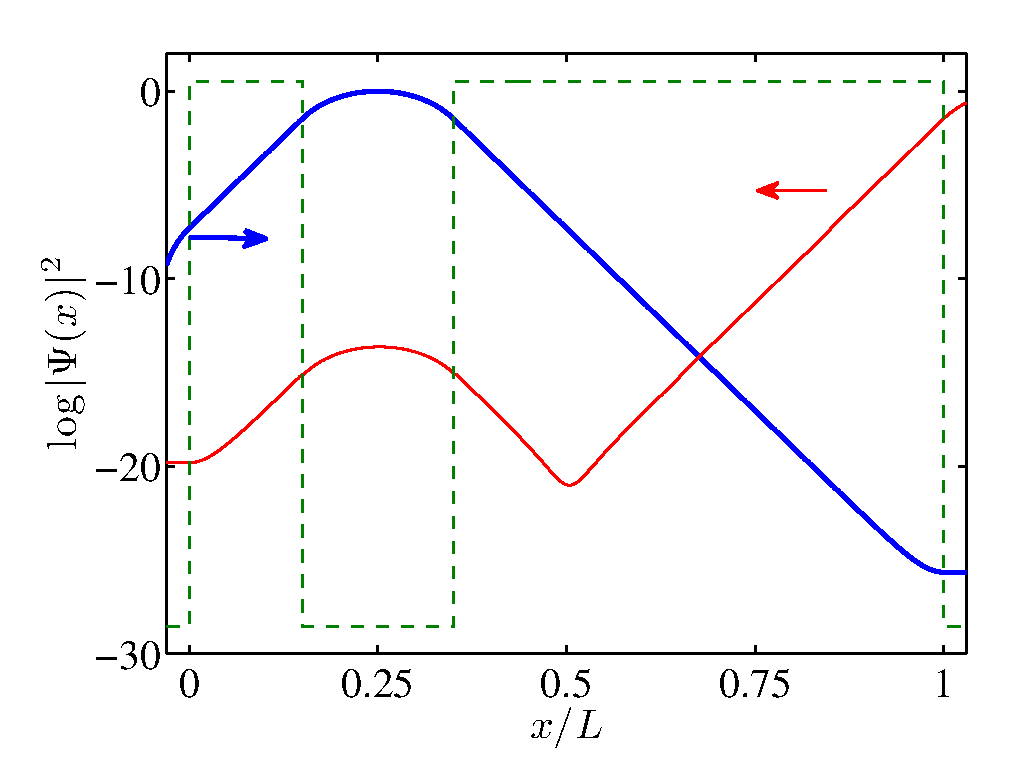
\includegraphics[width=3.25in]{chapters/Relation_between_transmission_and_energy_stored_in_random_media_with_gain__Phys_Rev_B/pictures/fig8_barrier_defect_at_14_and_34_waveform_log_chopped}}}
%\vskip -0.0in
%\scalebox{0.37}{\includegraphics{pictures/barrier_defect_at_14_and_34_waveform_log_chopped.eps}}
%\vskip -0.2in
\caption[Solution of the Schr\"{o}dinger equation for a potential barrier shown with the dashed line.]{Solution of the Schr\"{o}dinger equation for a potential barrier shown with the dashed line. The wavefunction is plotted at resonant energy of the quasi-bound state associated with the well inside the potential barrier. The obtained spatial dependence in cases of the wave incident from the left (thick line) and the right (thin line) are qualitatively similar to those in Fig.~\ref{fig:Efield_random}.\label{fig:barrierdefectlog}}
\end{figure}
%%%%%%%%%%%%%%%%%%%%%%%%%%%%%%%%%%%%%%%

The non-monotonic behavior of the wavefunction can be understood intuitively as follows. In the barrier regions there exist two eigen-solutions with exponentially increasing and exponentially decreasing amplitudes (in the electromagnetic problem, the envelope of the electric field plays the role of the amplitude). Balance between these two components is determined from the boundary conditions. It appears that in the $x_0=3L/4$ case, the exponentially increasing component has very small magnitude at the incident boundary, but becomes dominant at the turning point $x_T$. In contrast, when the defect lies close to the incident side, the exponentially increasing component is dominant starting at boundary of the sample.

The above observation confirms our results obtained using the random model in Sec.~\ref{sec:localization_passive}.

%\bibliography{2009_TE_prb.bbl}
%\bibliography{../../latex_bibliography}
%\bibliography{/home/alexey/SVN/research/latex_bibliography}

%\end{document}

\label{paper:1_end}

\PaperManuscript{2}{Classification of regimes of wave transport in \-non-\-con\-servative random media}
%Journal of Modern Optics (2010) doi:10.1080/09500340.2010.519443
% /svn/research/Project_Quasi1D_Transport/2010_Regimes_Plot_manuscript/2010_JMO/20100712_regimes_plot.tex
\setcounter{section}{0}
\setcounter{figure}{0}
\setcounter{table}{0}
\label{paper:2_start}
% \documentclass[]{tMOP2e}
% 
% \citestyle{tMOP}
% \begin{document}
% 
% \doi{10.1080/0950034YYxxxxxxxx}
% \issn{1362-3044}
% \issnp{0950-0340} \jvol{00} \jnum{00} \jyear{2010} \jmonth{25 January}

%\markboth{A. Yamilov and B. Payne}{Classification of regimes of wave transport in quasi one-dimensional non-conservative random media}
 
\chapter{Classification of regimes of wave transport in quasi one-dimensional non-conservative random media}
\label{chap:regimes}
\label{paper:2_start}

% \author{
% A. Yamilov$^\ast$ \thanks{$^\ast$Corresponding author. Email: yamilov@mst.edu \vspace{6pt}} and 
% B. Payne\\\vspace{6pt}  {\em{Physics Department, Missouri University of Science and Technology, Rolla, MO USA}}}
% 
\begin{center}
Alexey Yamilov$^1$ and Ben Payne$^1$
\end{center}

\ \\
\begin{center}
\textit{$^1$Department of Physics, Missouri University of Science \& Technology,\\ Rolla, MO 65409}
%$^2$Department of Applied Physics, Yale University, New Haven, CT 06520}
\end{center}

\ \\
% \maketitle
% \begin{abstract}
% 
\addcontentsline{toc}{section}{ABSTRACT}
\begin{center}\textbf{ABSTRACT\footnote{Published in Journal of Modern Optics (2010)}}        \end{center}

Passive quasi-one-dimensional random media are known to exhibit one of the three regimes of transport -- ballistic, diffusive or localized --  depending on the system size. In contrast, in non-conservative systems the physical parameter space also includes the gain/absorption length scale. Here, by studying the relationships between the transport mean free path, the localization length, and the gain/absorption length, we enumerate fifteen regimes of wave propagation through quasi-one-dimensional random media with gain or absorption. The results are presented graphically in a form of a phase diagram. Of particular experimental importance, in absorbing random medium we identify three different regimes which bear signatures of the localized regime of the passive counterpart. We also review the literature and, when possible, assign experimental systems to a particular regime on the diagram. 
% \begin{keywords} 
% Wave propagation in random media; diffusion; Anderson localization; random laser
% \end{keywords}
% \end{abstract}

\section{INTRODUCTION}
\label{sec:introduction}

Discovery of Anderson localization (AL)~\cite{1958_Anderson} served as a catalyst for interest in wave propagation through random media for over fifty years~\cite{2009_Lagendijk_PT}. AL is a wave phenomenon~\cite{2007_Akkermans_book} that results in cessation of diffusion~\cite{2010_Wolfle}. First conceived in electronic systems, it originates from  repeated self-interference of de Broglie waves during their propagation in a random potential. Conservation of number of carriers, enforced because the electrons possess a charge, lies in the foundation of the concept of AL~\cite{1991_Altshuler}. 

Understanding the effect of absorption~\cite{1984_John_prl}, ubiquitous in optical systems, turned out to be essential for proper physical description and interpretation of experimental studies of localization of {\it light}~\cite{1989_Genack,1997_wiersma_nature,1999_Maret,2000_chabanov_nature,2007_Maret,2007_Segev} and other classical waves such as ultrasound~\cite{2008_van_Tiggelen_Nature,2008_Weaver}. It also prompted~\cite{2000_chabanov_nature} the search for alternative criteria of localization in absorbing media. Furthermore, the effect opposite to the absorption, coherent amplification, leads to an altogether new wave phenomenon of random lasing with a host of potential applications~\cite{2005_Cao,2008_Wiersma}. The multitude of the observed phenomena in realistic disordered optical systems, which are inevitably absorbing or can even be made amplifying, suggests that AL phenomenon is intrinsically more complex in non-conservative random media. It motivates refinement of the very concept of AL and its criteria in such systems~\cite{2010_Payne_loc_criterion}.

In this work, with the goal of establishing a criterion of Anderson localization in non-conservative quasi-one-dimensional (quasi-1D) random media, such as disordered waveguides, we map out the two-dimensional parameter space of the problem that consists of the system size and gain or absorption length. In quasi-1D geometry the transition to AL lacks sharp features (mobility edges) observed in even more complex three-dimensional systems. Thus,  Section \ref{sec:q1d_localization} is devoted to a discussion of Anderson localization in quasi-1D random media. In Section \ref{sec:parameters} we review and formally define the parameters that characterize quasi-1D non-conservative systems. In Section \ref{sec:phases}, by studying the relationships between these parameters we identify fifteen different regimes of wave transport in the parameter space. Furthermore, we review the available publications on the subject and, when published data is sufficient, assign them to a particular region on our phase-diagram. We conclude with a discussion of the results obtained in Section \ref{sec:discussion_regimes}.

\section{LOCALIZATION IN QUASI-1D NON- CONSERVATIVE RANDOM MEDIA}
\label{sec:q1d_localization}

\subsection{Localization in Finite Passive Random Media}

Anderson localization can be defined in a strict mathematical sense in random media with infinite dimensions~\cite{2010_Spencer}. In experimentally relevant situations, one usually deals with finite systems that are characterized by non-zero wave flux at the boundaries. Thus, a study of localization in finite systems is an analysis of transport through random media. 

The dimensionless conductance averaged over an ensemble of macroscopically equivalent, but microscopically different disorder realizations, $g$, can be used as a criterion that defines the onset of localization~\cite{1977_Thouless}. According to scaling theory of localization~\cite{1979_Anderson}, $g$  uniquely determines  evolution of its entire distribution with an increase of the system size, formally described by the scaling function~\cite{2010_Kramer}. Thus, the scaling theory provides an important link between finite and the infinite systems.

\subsection{Localization in Finite Random Media With Gain or Absorption}

Transmittance is the electromagnetic counterpart of conductance~\cite{1988_Stone}. This analogy with mesoscopic electronic transport makes it tempting to adopt the localization criteria (LC) based on $g$ in optical systems. However, the LC developed for passive systems are not necessarily applicable for non-conservative random media, where the extrapolation to infinite size becomes problematic~\cite{1999_van_Tiggelen}. The scaling function is no longer a single parameter function~\cite{1994_Freilikher_absorption}. Indeed, in absorbing systems $g\ll 1$ may not be indicative of the presence of localization~\cite{1998_Brouwer,2000_chabanov_nature}, and $g\gg 1$ in an amplifying random medium may not necessarily preclude occurrence of certain effects characteristic of localized systems~\cite{2004_Yamilov_intensity,2006_Yamilov_conductance}. Therefore, studies of localization in non-conservative systems concentrated on detecting the signatures of AL such as enhanced fluctuations~\cite{1994_Kumar,1995_Zhang,1996_Paasschens_gain,1997_Freilikher_gain,1998_Maret_PRL,2000_chabanov_nature,2006_Yamilov_conductance}, rounding of the coherent back scattering cone~\cite{1997_Wiersma_cbs,1999_Kaiser_cbs,2009_Maret}, anomalous diffusion~\cite{1989_Genack,1997_wiersma_nature,2006_Maret,2007_Segev,2008_van_Tiggelen_Nature,2009_Genack_PRB} and others.

In the case of absorption, a quantitative criterion, based on the magnitude of {\it fluctuation} of transmission normalized by its average, was put forward~\cite{2000_chabanov_nature}. Although it described the experiment well, the assumed critical value of fluctuations is somewhat subjective. In view of the fact that single parameter scaling is no longer applicable in presence of absorption~\cite{1994_Freilikher_absorption}, it remains an open question whether the same criterion would be suitable for systems with different values of absorption. 

In random media with gain, the situation is further complicated because within the statistical ensemble there always exists a non-zero probability of encountering a special realization of disorder where the given value of the gain parameter exceeds threshold for random lasing. Without saturation effects, such a realization will have an infinite contribution to the statistical average. Inclusion of saturation introduces dependence on system- and material-specific parameters which are not associated with wave-transport properties of the random medium. To regularize the statistical ensemble, conditional statistical averaging was introduced by excluding the diverging contributions~\cite{2005_Yamilov_correlations}. Such an approach turned out to be fruitful in studies of enhanced fluctuations and  correlation in mesoscopic transport of the electromagnetic waves through random media with optical amplification~\cite{2004_Yamilov_intensity,2006_Yamilov_conductance,2005_Yamilov_correlations}. It was found that the correlation linewidth $\delta\omega$~\cite{2000_Sebbah} obtained in such an ensemble can be used to define the Thouless parameter $\delta=\delta\omega/\Delta\omega$ in random media with gain. Here $\Delta\omega$ is the average mode spacing which is equal to the reciprocal of the density of states in the system.  Reduction of $\delta$ correlates well~\cite{2005_Yamilov_correlations} with the enhancement of mesoscopic fluctuations -- another signature of AL. These investigations motivated us to explore an intriguing possibility of localization by gain -- enhancement of the mesoscopic phenomena with an increase of the amplification strength. Because the dimensionless conductance and Thouless parameter exhibit opposite trends with an increase of gain, the relationship $g=\delta$ is no longer valid in non-conservative media. This observation exemplifies added complexity in description of wave propagation in open random media with gain (or absorption), even when such effects as gain saturation or spontaneous emission noise (see e.g. Refs.~\cite{1999_Patra_noise,2009_Skipetrov_noise}) are not accounted for.

\subsection{Disordered Waveguide (Wire) Geometry}

Because of quantization of the transverse component of momentum, the transport properties in quasi-1D (waveguide)  geometry can be conveniently described in terms of a transfer matrix~\cite{1997_Beenakker}. Assuming that this transfer matrix has random entries with only flux and symmetry conservation turned out to be a fruitful approach~\cite{2004_Mello_Kumar_book} which yielded some exact analytical results~\cite{1994_Beenakker_exact,2000_Mirlin}.

In passive quasi-1D systems the transition from ballistic to diffusive and then to localized regimes occurs as a function of the system size $L$ only (and not the strength of disorder as in three-dimensions, 3D), even if the system is weakly scattering $k\ell\gg 1$. The diffusion regime is only a transitive regime which, unlike in 3D systems, does not persists in the limit $L\rightarrow\infty$. Therefore, quasi-1D systems 
\cite{1995_Kogan,1996_Paasschens_gain,1998_Brouwer,1998_Birman_waveguide,1998_Maret_PRL,1999_Muttalib,
2000_chabanov_nature,2002_Saenz_g,2005_Markos,2005_Genack_review,2006_Yamilov_conductance,2007_Botten_waveguide,
2007_Froufe-Perez_PRE,2007_deMatos_random_fiber_laser} do not exhibit critical behavior at the size-driven transition from diffusive to localized transport. However, because we set out to consider the non-conservative systems for which $L\rightarrow\infty$ may not be easily defined, quasi-1D geometry is sufficiently complex to capture both diffusive and localized behavior in systems of {\it finite size}. As shown below, it is expected to exhibit very complex parameter space, c.f. Fig.~\ref{fig:phase_space}. Furthermore, due to the availability of the ever more powerful computational resources, it has recently become possible to perform systematic numerical investigations of the entire parameter space of the quasi-1D non-conservative random media. 

Although an interplay between the effects of amplification and localization has been subject of continuous research effort (see e.g. Refs.~\cite{1994_Kumar,1995_Zhang,1995_zyuzin_fluctuations,1996_Paasschens_gain,1997_Freilikher_gain,1997_Wiersma_cbs,
2000_Cao_localization,2001_Soukoulis_modeDist,2001_Sebbah_FDTD,2004_Yamilov_intensity,2005_Genack_Milner,
2005_Apalkov_corr,2005_Yamilov_correlations,2006_Heinrichs,2006_Yamilov_conductance,2008_Stone,2008_Conti_opals,
2009_Frank,2010_Payne_PRL}), a systematic study which would rationalize different theoretical and experimental observations has not yet been attempted. Below, we present such a systematic analysis of the parameter space for quasi-1D non-conservative random media.

%-----------------------------------------------
\section{DEFINITIONS OF PARAMETERS IN QUASI-1D NON- CONSERVATIVE RANDOM MEDIA}
\label{sec:parameters}
%-----------------------------------------------

% %%%%%%%%%%%%%%%%%%%%%%%%%%%%%%%%%%%%%%%%%%%%
% \begin{figure}
% \vskip -0.2cm
% \centerline{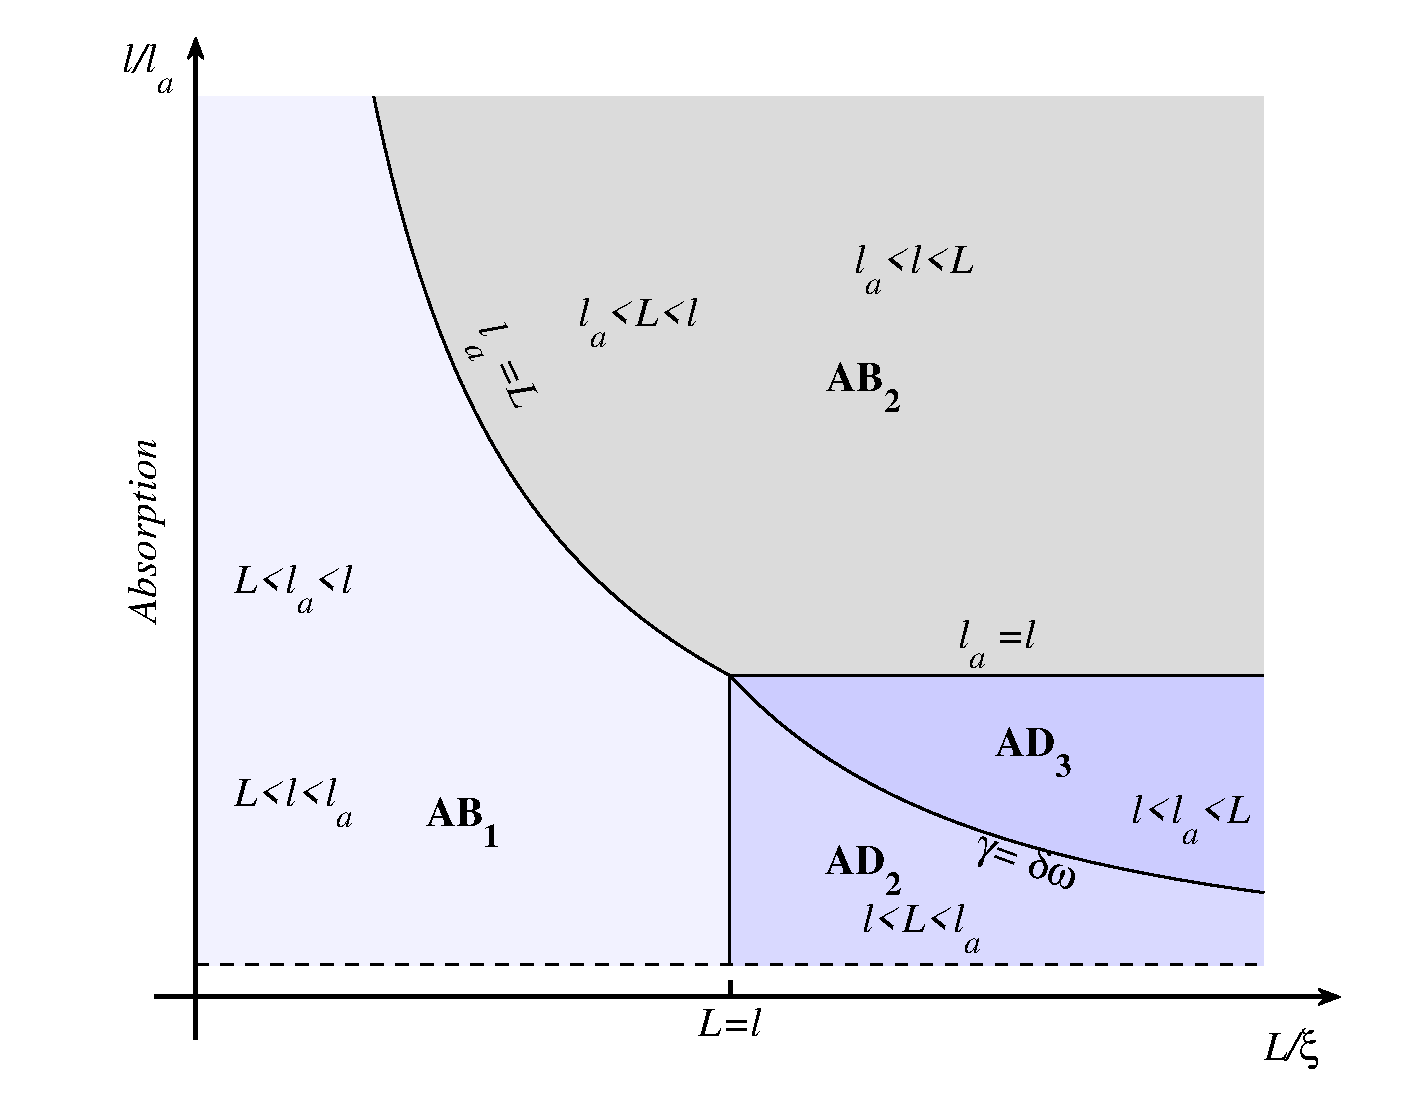
\includegraphics[width=4in]{chapters/Classification_of_regimes_of_wave_transport_in_non-conservative_random_media__J_Mod_Optics/pictures/fig1a_regimes_plot_upper}}
% \vskip -0.8cm
% \hskip -0.1cm
% \centerline{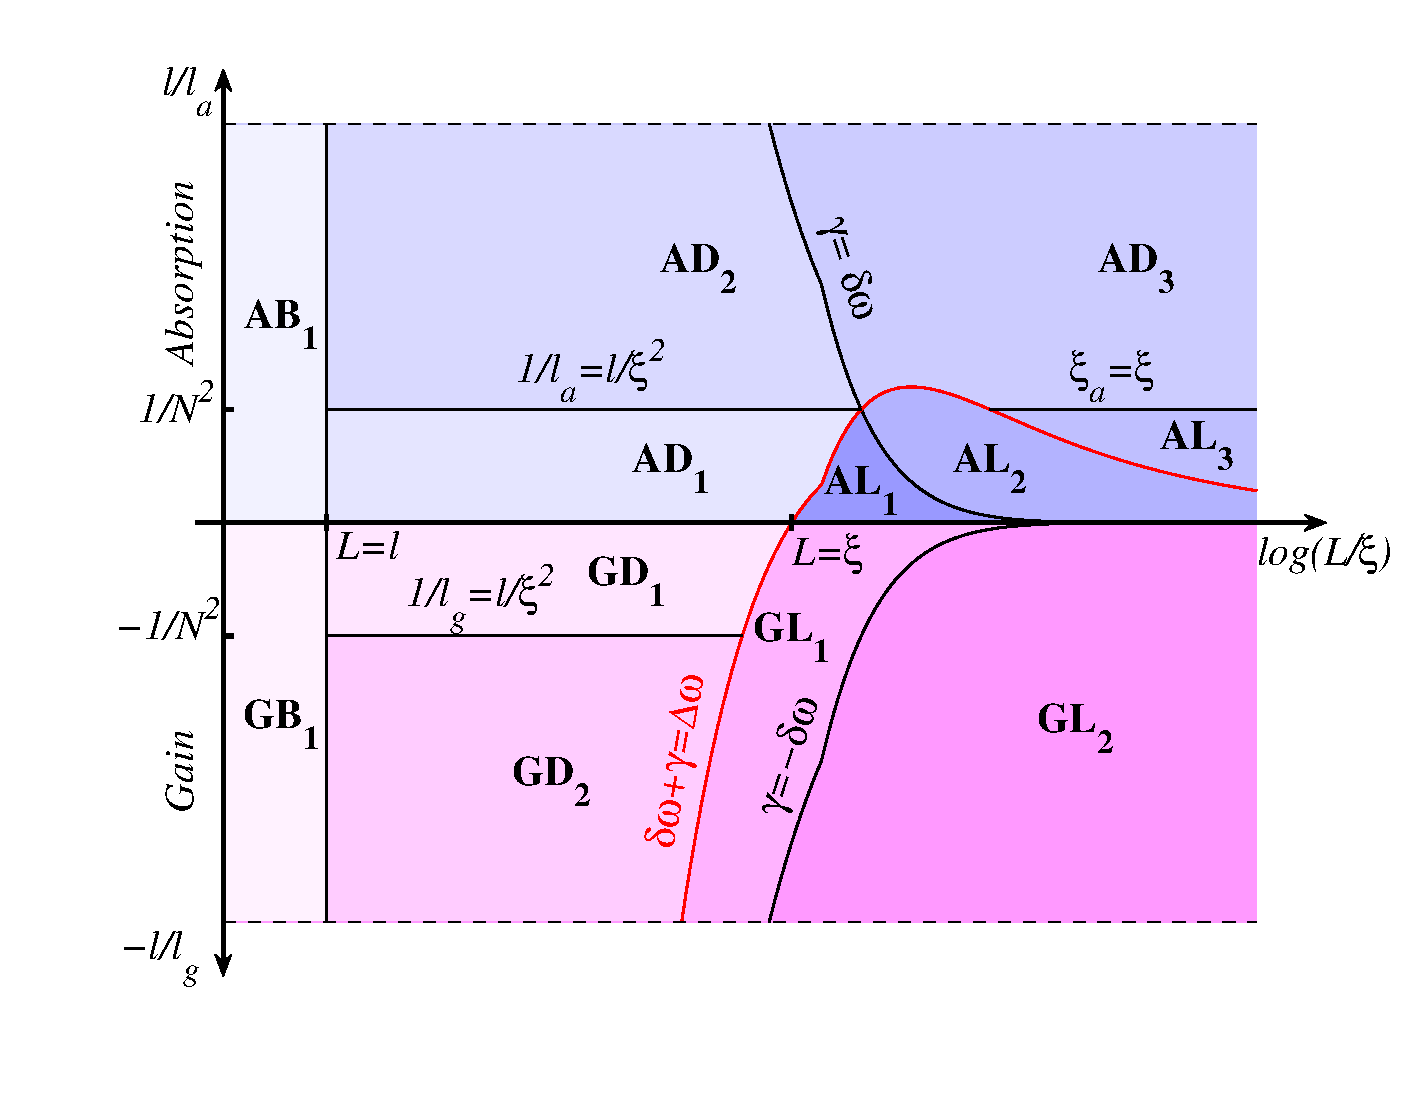
\includegraphics[width=4.15in]{chapters/Classification_of_regimes_of_wave_transport_in_non-conservative_random_media__J_Mod_Optics/pictures/fig1b_regimes_plot_main}}
% \vskip -0.6cm
% \centerline{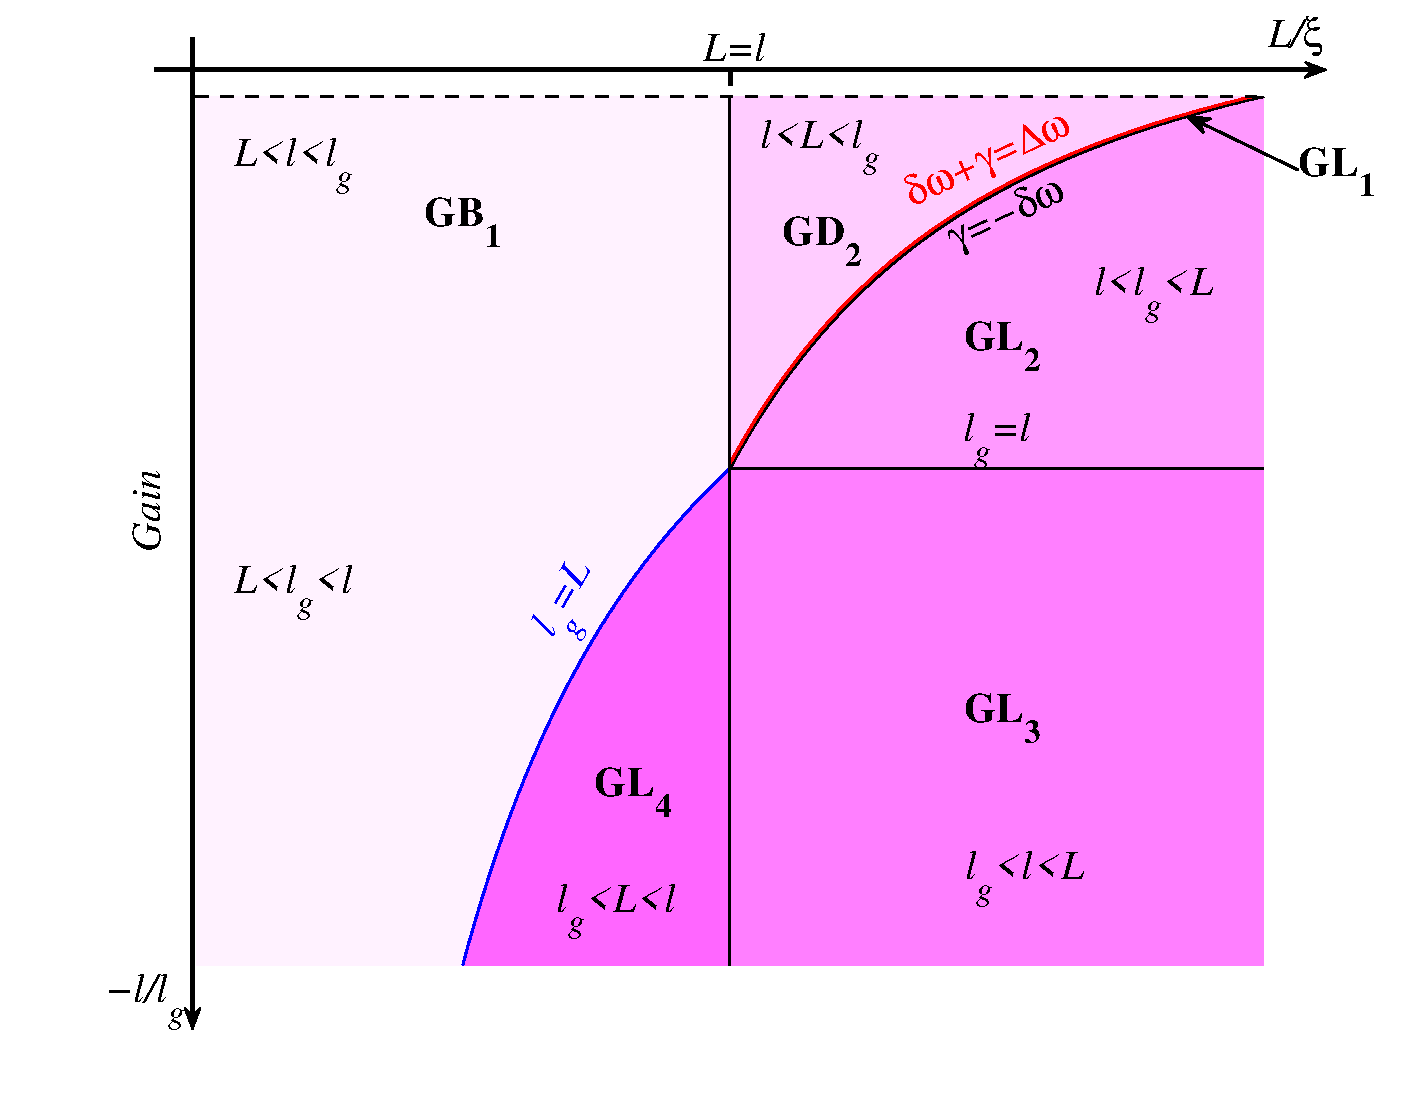
\includegraphics[width=4in]{chapters/Classification_of_regimes_of_wave_transport_in_non-conservative_random_media__J_Mod_Optics/pictures/fig1c_regimes_plot_lower}}
% \vskip -0.2cm
% \caption[Classification of regimes of wave transport in quasi-1D non-conservative random media.]{\label{fig:phase_space} Classification of regimes of wave transport in quasi-1D non-conservative random media. X and Y axes correspond to the system length $L$ and absorption/gain length $\ell_{a,g}$, see text for labeling convention. Due to large disparity in the characteristic length scales, the plot is separated into three panels which correspond to strong absorption $1/\ell_a\sim 1/\ell$ (upper panel), weak absorption and gain $1/\ell_{a,g}\sim \ell/\xi^2$ (middle panel), and strong gain $1/\ell_g\sim 1/\ell$ (lower panel) regimes. }
% \end{figure}
% %%%%%%%%%%%%%%%%%%%%%%%%%%%%%%%%%%%%%%%%%%%%%

%%%%%%%%%%%%%%%%%%%%%%%%%%%%%%%%%%%%%%%%%%%%
\begin{figure}
\vskip -0.2cm
\centerline{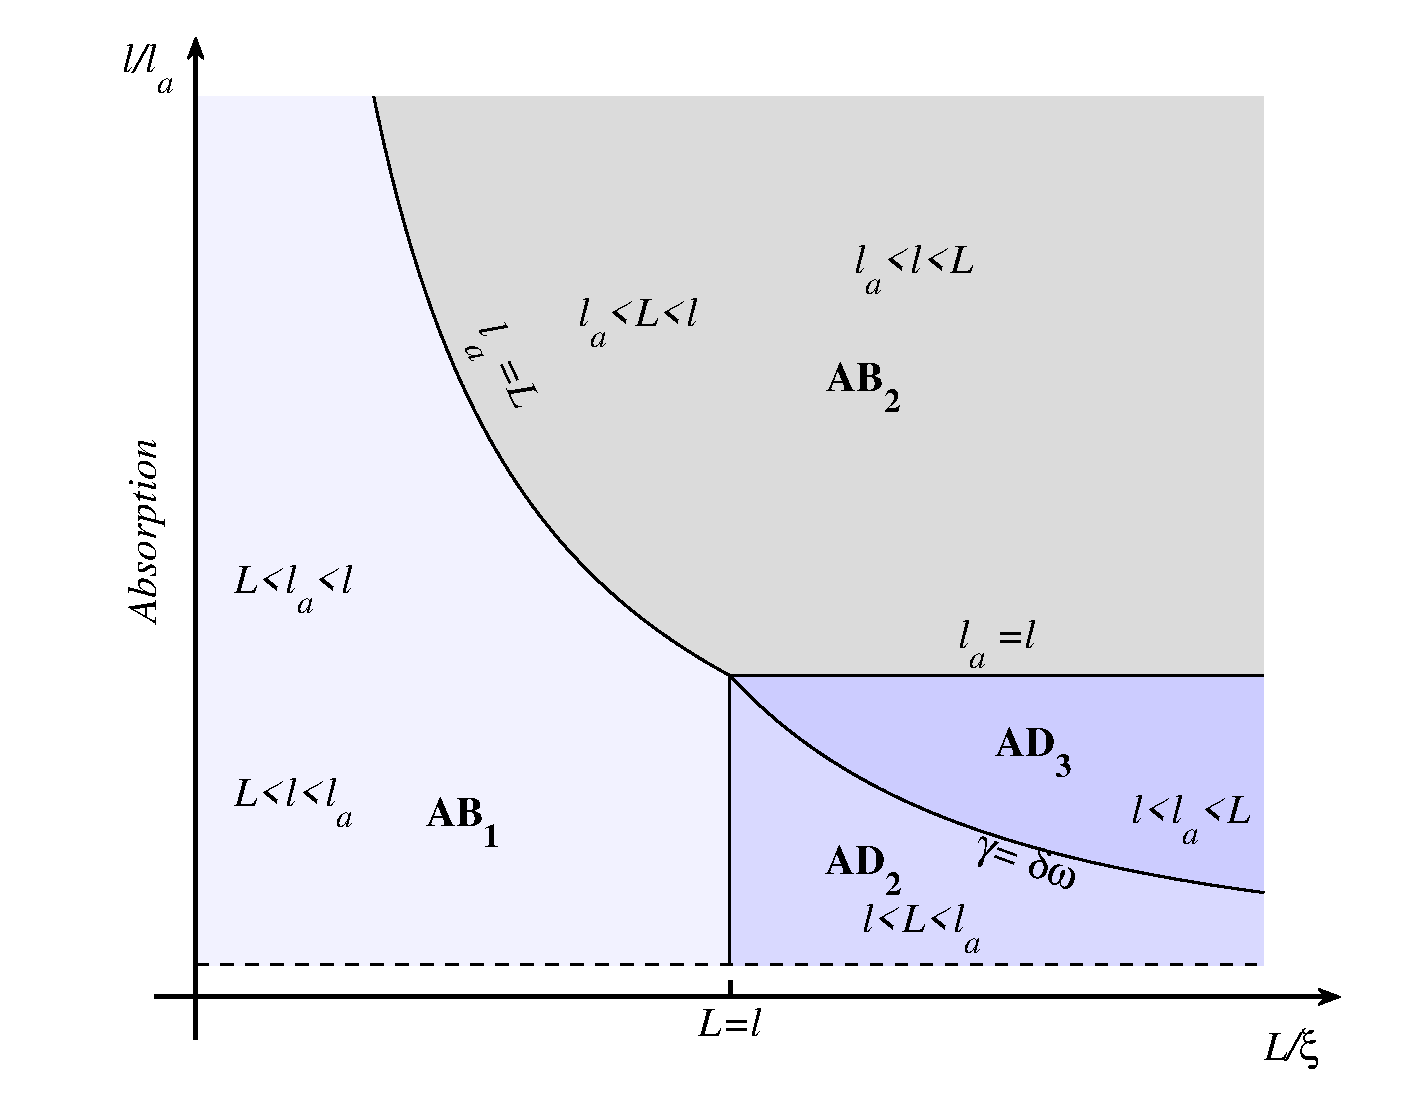
\includegraphics[width=4in]{chapters/Classification_of_regimes_of_wave_transport_in_non-conservative_random_media__J_Mod_Optics/pictures/fig1a_regimes_plot_upper}}
\vskip -0.2cm
\caption[Classification of regimes of wave transport in quasi-1D non-conservative random media; upper panel.]{Classification of regimes of wave transport in quasi-1D non-conservative random media; upper panel.}
\end{figure}

\begin{figure}
\hskip -0.1cm
\centerline{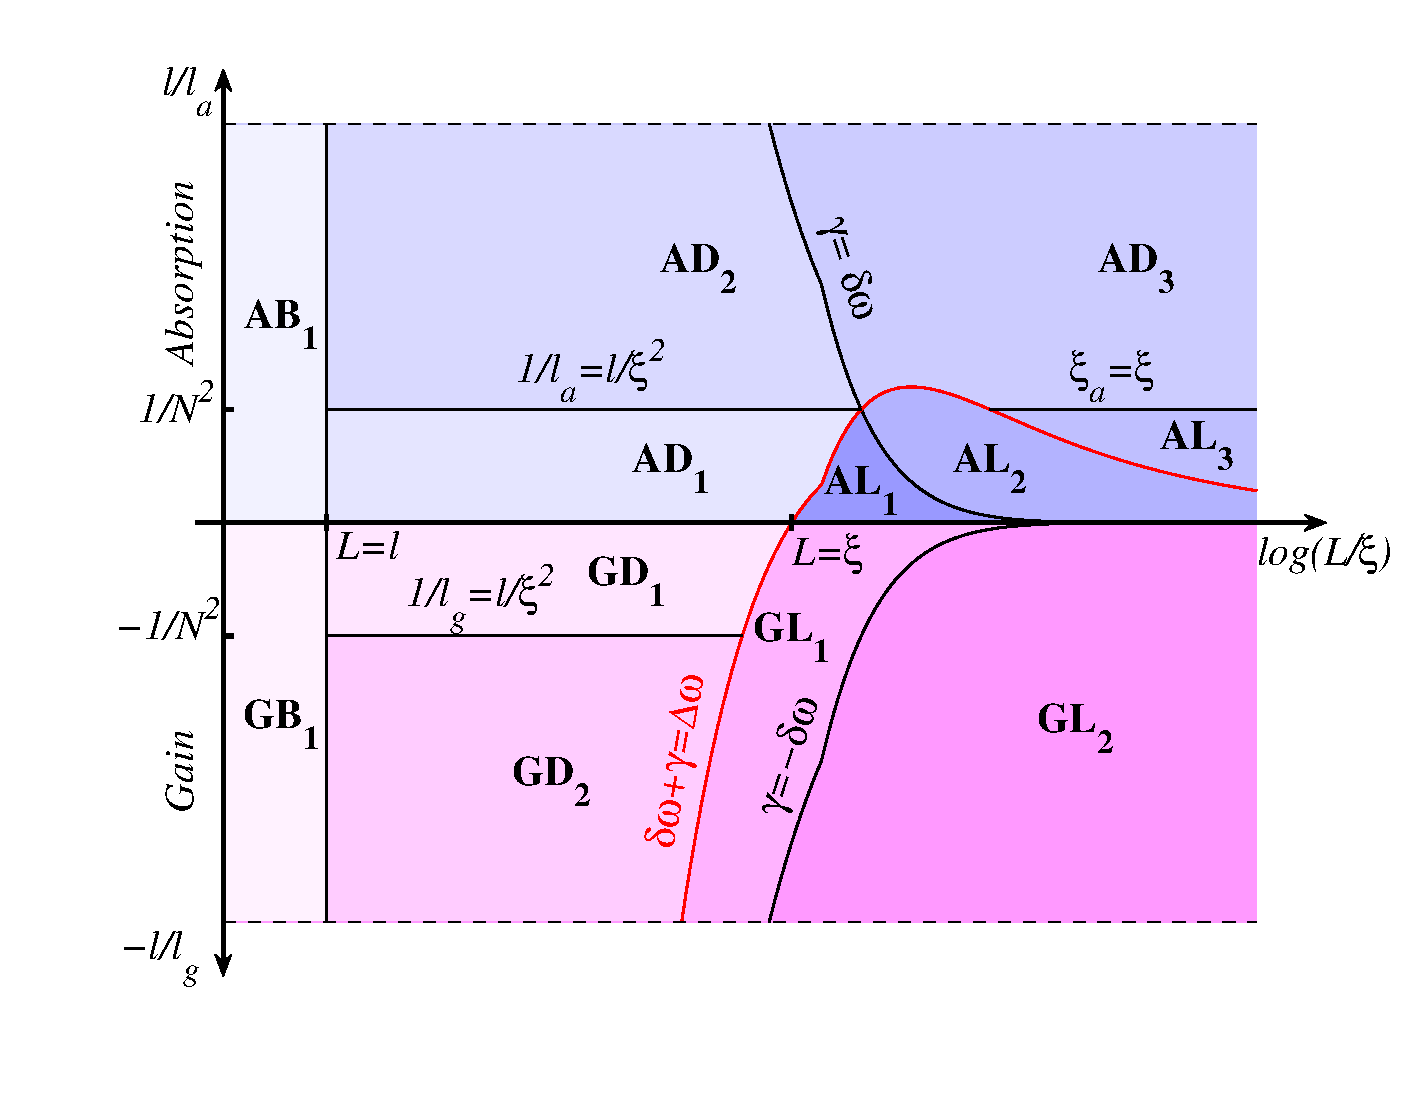
\includegraphics[width=4.15in]{chapters/Classification_of_regimes_of_wave_transport_in_non-conservative_random_media__J_Mod_Optics/pictures/fig1b_regimes_plot_main}}
\caption[Classification of regimes of wave transport in quasi-1D non-conservative random media; middle panel.]{Classification of regimes of wave transport in quasi-1D non-conservative random media; middle panel.}
\end{figure}

\begin{figure}
\vskip -0.6cm
\centerline{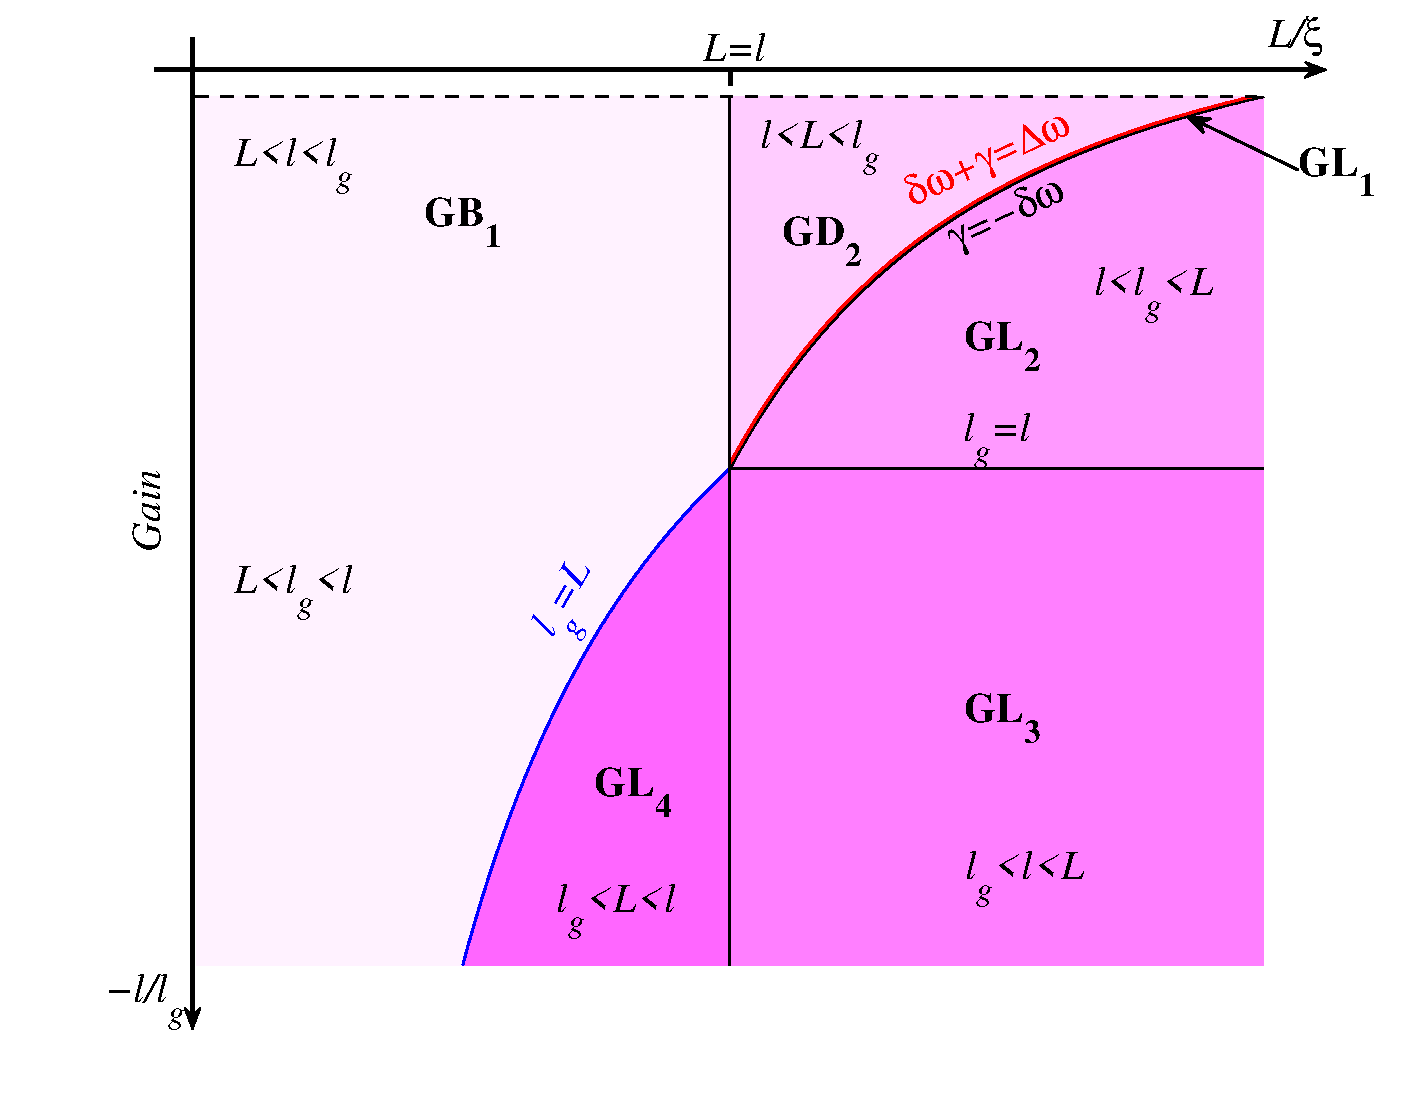
\includegraphics[width=4in]{chapters/Classification_of_regimes_of_wave_transport_in_non-conservative_random_media__J_Mod_Optics/pictures/fig1c_regimes_plot_lower}}
\vskip -0.2cm
\caption[Classification of regimes of wave transport in quasi-1D non-conservative random media; lower panel.]{\label{fig:phase_space} Classification of regimes of wave transport in quasi-1D non-conservative random media; lower panel. X and Y axes correspond to the system length $L$ and absorption/gain length $\ell_{a,g}$, see text for labeling convention. Due to large disparity in the characteristic length scales, the plot is separated into three panels which correspond to strong absorption $1/\ell_a\sim 1/\ell$ (upper panel), weak absorption and gain $1/\ell_{a,g}\sim \ell/\xi^2$ (middle panel), and strong gain $1/\ell_g\sim 1/\ell$ (lower panel) regimes. }
\end{figure}
%%%%%%%%%%%%%%%%%%%%%%%%%%%%%%%%%%%%%%%%%%%%%

In passive volume-disordered waveguides, the transition from ballistic to diffusive and then to the localized regime occurs when the length of the system is increased above $\ell$ and $\xi=N\times\ell$ respectively. Here $\ell$ is the transport mean free path, $N$ is the number of waveguide channels, and $\xi$ is the localization length~\cite{1997_Beenakker}. In waveguides filled with a non-conservative random medium, the parameter space becomes two-dimensional: beside the system size $L$, it also includes the gain or absorption length scale $\ell_{g,a}$. Fig.~\ref{fig:phase_space} shows this two-parameter phase space.

The boundaries between different regions in Fig.~\ref{fig:phase_space} are based on relationships between a subset of parameters which can be expressed in terms of length or time scales. The length parameters include $L$, $\ell$, $\xi$, and (ballistic) absorption/gain lengths $\ell_a/\ell_g$. The other set of boundaries are more physically transparent when expressed in the spectral domain in terms of the following parameters: the average mode spacing $\Delta\omega\propto (NL)^{-1}$; the passive average mode linewidth $\delta\omega$ ($\propto DL^{-2}$ in diffusive regime $\ell<L<\xi$); and gain or absorption rate $\gamma_{g,a}=\mp c/\ell_{g,a}\equiv\mp\tau_{g,a}^{-1}$ (negative in the case of gain). Here, $c$ is speed of light and $D$ is the diffusion constant. Based on these parameters the following relationships can be established:
\begin{quote}
$\bullet$ $L\sim\ell$ signifies the transition from ballistic to multiple-scattering regime. No other significant changes are expected in the region of moderate absorption/gain $\ell<\ell_{g,a}$ shown in the middle panel in Fig.~\ref{fig:phase_space};\\
$\bullet$ Generalized Thouless parameter $\delta\omega(\gamma)/\Delta\omega\simeq(\delta\omega+\gamma)/\Delta\omega$ describes~\cite{2005_Yamilov_correlations} the transition from spectrally overlapping quasi-modes to the resonance-dominated behavior. Here $\delta\omega\equiv\delta\omega(\gamma=0)$. In the case of passive system $\gamma=0$, the ratio reduces to $\delta=g$;\\
$\bullet$ $|\gamma|=\delta\omega$ curves signify the transition to the regime when the gain or absorption overcomes the radiative leakage of an average quasi-mode in the system;\\
$\bullet$ Long self-crossing Feynman paths give rise to weak localization correction. In quasi-1D, the probability of such paths becomes equal to unity at $L=\xi$, their length is given by $L^2/\ell=\xi^2/\ell$. Therefore, we estimate that the weak localization corrections become susceptible to gain or absorption when $\ell_{g,a}$ becomes comparable to this length scale;\\
$\bullet$ Condition $\ell=\ell_{g,a}$ marks the onset of the regimes of very strong absorption/gain shown in the upper/lower panel in Fig.~\ref{fig:phase_space}. Here, the ballistic regimes become limited by the condition $\ell_{g,a}=L$.\\
\end{quote}
\noindent The distinctions between different regions are only valid in the statistical sense because the sample-to-sample fluctuations are inherent in a random medium. When gain is present, the statistical ensemble is assumed to be conditional~\cite{2005_Yamilov_correlations}, which excludes the non-physical solutions~\cite{2002_Zhang_phys_solutions}. Furthermore, the considered (open) system is of a finite size and, therefore, the transitions between different ``phases'' are expected to be smooth. Hence, our diagrams should only be used as a guide to identify qualitatively different regimes of wave transport.

\section{``PHASES'' OF WAVE TRANSPORT THROUGH \\NON-CONSERVATIVE RANDOM MEDIA} 
\label{sec:phases}

The regions in Fig.~\ref{fig:phase_space} are labeled with two letters and a subscript. The first letter, $A/G$, stand for {\underline a}bsorption/{\underline g}ain and is common for all regions above/below the horizontal axis. The second letter in the labels, $B$, $D$ or $L$, is attributed to the regimes where some signatures of the {\underline b}allistic, {\underline d}iffusive, and {\underline l}ocalized transport are expected to occur. Based on the list of separatrices listed above, one can identify the following regions:
\begin{quote}
$\bullet$ $GB_1,AB_1$: Random systems with parameters in these regions are expected to behave similar to their passive counterparts. Note that in the regime of very strong gain or absorption, $\ell_{g,a}^{-1}>\ell^{-1}$, the ballistic region becomes bounded by $L<\ell_{g,a}$;\\
$\bullet$ $GD_1,AD_1$: With exception of anomalously localized states~\cite{1991_Altshuler,1995_Muzykantskii_ALS,2000_Mirlin,2000_Cao_localization,2002_Apalkov_ALS,2004_Burin_ALS}, the gain or absorption is not expected to be sufficient to appreciably modify the diffusive behavior in these regions; \\
$\bullet$ $GD_2$: Such systems were successfully treated with the ``negative absorption'' diffusive approach often invoked in discussion of random lasers~\cite{1968_Letokhov,1994_lawandy_nature,1996_John_RandLaser,1996_Wiersma_RandomLaser,1996_Genack_DiffRandomLaser,
1999_Cao_RandomLaserPRL,1999_Vardeny_PolymerRandomLaser,2001_vansoest_thesis,2004_Florescu}. Systems in this regime also are expected to exhibit the enhanced mesoscopic fluctuations and non-local correlations~\cite{2005_Yamilov_correlations,2004_Yamilov_intensity,2006_Yamilov_conductance};\\
$\bullet$ $GL_1$: Random media with such strong gain, $\delta\omega(\gamma)/\Delta\omega<1$, are expected to exhibit resonant features in spectrum with strong sample-to-sample fluctuations~\cite{1995_zyuzin_fluctuations,1997_Burkov_Zyuzin}. Retaining the contribution from only the physical solutions becomes essential~\cite{1999_Jiang,2002_Zhang_phys_solutions} for the systems with the parameters in this region;\\
$\bullet$ $GL_2$: The condition $\gamma_g=-\delta\omega(\gamma =0)$ signifies lasing of an average mode and, in diffusive systems, is equivalent to the onset random lasing as predicted by Letokhov~\cite{1968_Letokhov}; \\
$\bullet$ $AL_1,AL_2,AL_3$: These regimes represent the systems which would formally be localized if the absorption could be removed. Of these, $AL_1$ is the most favorable case because the systems in this regime have spectrum of separated resonances, $\delta\omega(\gamma)/\Delta\omega\simeq(\delta\omega(\gamma=0)+\gamma)/\Delta\omega<1$, with the radiative leakage being the dominant relaxation mechanism (possibly, experimental systems of~\cite{2000_chabanov_nature} belong to this parameter ``phase''). The latter is no longer true for $AL_2$ regime. $AL_3$ describes an intriguing type of a random medium with a continuous spectrum due to strong absorption which has washed out the individual resonances, but still exhibiting the weak localization corrections;\\
$\bullet$ $AD_2,AD_3$: Systems in these regimes of moderate and strong absorption are expected to exhibit suppressed localization effects~\cite{1998_Brouwer}. For strong absorption, even the diffusion propagation is suppressed on long scales. The majority of experimental systems are expected to fall in one of these two regions;\\
$\bullet$ $AB_2$: This regime is marked by the dominant effect of absorption when $\ell_a$ is the shortest of all length-scales. Because it also implies $\ell_a^{-1}>\ell^{-1}$, diffusion-like propagation does not sets in;\\
$\bullet$ $GL_3,GL_4$: In these regimes, similar to $GL_2$, it is more meaningful to ascribe $L$ notation to {\underline l}asing. In contrast to the very strong absorption counterpart $AB_2$, we separated $\ell_g^{-1}>\ell^{-1}$ region into $\ell_g<\ell<L$ ($GL_3$) and $\ell_g<L<\ell$ ($GL_4$). In the latter regime, one can justify neglecting scattering. Thus, $GL_4$ encompasses lasing phenomena in Fabry-Perot geometry. In contrast, in $GL_3$ the scattering can provide the dominant feedback as it has been very recently demonstrated experimentally~\cite{2006_Wu,2006_Wu_spie}.\\
\end{quote}
% Unlike the absorbing systems where one loc-abs, gain diff-loc\\

\section{DISCUSSION AND OUTLOOK}
\label{sec:discussion_regimes}

As it was discussed in the previous section, the parameter space in volume-disordered waveguides becomes two-dimensional when the medium is no longer assumed passive. Importantly, the coherent amplification/absorption non-trivially affects the interferences of multiply-scattered waves and, thus, can promote/suppress localization phenomena. This observation has motivated us to begin to systematically explore an intriguing possibility of localization by gain enhancement of the mesoscopic phenomena with an increase of the amplification strength~\cite{1995_zyuzin_fluctuations,1997_Burkov_Zyuzin,2004_Yamilov_intensity,2005_Yamilov_correlations,2006_Yamilov_conductance,2010_Payne_loc_criterion,2010_Payne_TE}. Furthermore, in the experimental studies of localization of light, the importance of the proper account of absorption has been widely appreciated~\cite{1991_Genack,1997_wiersma_nature,1999_Maret,2000_chabanov_nature,2006_Maret}. 

In finite {\it passive} random media, the prevalence of the localization effects can be assessed with a number of criteria: averaged dimensional conductance, its mesoscopic fluctuations relative to the mean value, Thouless parameter, renormalization of the diffusion coefficient, inverse participation ratio, spatial correlations and others. Single parameter scaling theory of localization may be used to establish the relationships between different criteria. These relationships will not necessarily hold in the non-conservative media. We believe that our analysis of the parameter space in Sec.~\ref{sec:phases} will be instrumental in generalizing the concept of AL and establishing a robust criterion for its observation in {\it non-conservative} random media~\cite{2010_Payne_loc_criterion,2010_Payne_TE}.

\section{ACKNOWLEDGMENTS}
This work was supported by National Science Foundation Grant No. DMR-0704981. 
%The numerical results that contributed to this work were obtained at the Tera-Grid, award no. DMR-090132.

% \bibliographystyle{tMOP}
% %\bibliography{C:/SVNr/research/latex_bibliography}
% \bibliography{20100712_regimes_plot.bbl}

%\end{document}

\label{paper:2_end}


\PaperManuscript{3}{Near-field effects in wave transport through in disordered waveguides}
% to be submitted
% /svn/research/Project_Quasi1D_Transport/2012_Closed_Channels_manuscript/
\setcounter{section}{0}
\setcounter{figure}{0}
\setcounter{table}{0}
\label{paper:3_start}
% %\RequirePackage{lineno}
% 
% %\documentclass[aps,prb,superscriptaddress,showpacs,amsmath,amssymb,letterpaper,preprint]{revtex4}
% %\documentclass[aps,prb,superscriptaddress,showpacs,amsmath,amssymb,letterpaper]{revtex4}
% %\documentclass[aps,prb,superscriptaddress,showpacs,amsmath,amssymb,letterpaper,twocolumn]{revtex4}%floatfix
% 
% % https://authors.aps.org/revtex4/revtex4_faq.html#u1
% % use the following for a one-column, double-spaced, 12 pt document
% %\documentclass[preprint,prb,         showpacs,amsmath,amssymb]{revtex4-1}
% 
% % use the following for the published layout
% \documentclass[reprint,pra,         showpacs,amsmath,amssymb]{revtex4-1}
% 
% %For APS journals, only the prb option gives superscript-style citations.
% 
% \usepackage{mciteplus} % for bibliography style ``apsrevM''
% %\usepackage{dcolumn}
% \usepackage{graphicx}
% \usepackage{epsfig,color,verbatim} % multi-line comments
% \usepackage{subfigure}             % allows for use of "sub figure" 1a, 1b, etc
% \usepackage{hyperref}
% 
% %\linenumbers
% 
% \usepackage{amsmath} % advanced math
% \usepackage{appendix}
% %\usepackage[backref, colorlinks=false, pdftitle={Correction to the single scatterer quasi-1D models}, pdfauthor={Tom Mahler, Ben Payne, Alexey Yamilov}, pdfsubject={for publication}, pdfkeywords={localization, transmission, random, media}]{hyperref}
% \begin{document}
% 
\chapter{Near-field effects in wave transport through in disordered waveguides}
\label{chap:closed_channels}
\label{paper:3_start}

\begin{center}
Ben Payne$^1$, Tom Mahler$^1$, and Alexey Yamilov$^1$
\end{center}

\ \\
\begin{center}
\textit{$^1$Department of Physics, Missouri University of Science \& Technology,\\ Rolla, MO 65409}
%$^2$Department of Applied Physics, Yale University, New Haven, CT 06520}
\end{center}

\ \\
% \author{Ben~Payne, %\footnote{Electronic~address:~benjamin.payne@mst.edu},
% Tom~Mahler, %\footnote{Electronic~address:~tom.mahler@mst.edu},
% Alexey~G.~Yamilov\footnote{Electronic~address:~yamilov@mst.edu}}
% \affiliation{Department of Physics, Missouri University of 
% Science \& Technology, Rolla, MO 65409}
% \date{\today}
% 
% \begin{abstract}
\addcontentsline{toc}{section}{ABSTRACT}
\begin{center}\textbf{ABSTRACT\footnote{In preparation for Physical Review B (2012).}}        \end{center}

Evanescent coupling between scatterers in the course of wave propagation through random media is a notoriously difficult problem. Commonly these near-field effects are not considered explicitly. Instead, a phenomenological parameter, transport mean free path, is introduced. This treatment is sufficient to describe the macroscopic wave transport as exemplified by the success of Dorokhov and Mello, Pereyra, and Kumar (DMPK) theory. 
% 
% % OLD:
% %In models of transport in quasi-1D waveguides with random media such as that of Dorokhov and Mello, Pereyra, and Kumar, evanescent channels have been not included. Work by Bagwell and others has demonstrated that for a single scatterer inclusion of evanescent channels can be reduced to equivalent systems with only propagating channels, renormalizing scattering length. Here we show that evanescent channels can be analytically accounted for by renormalization of transfer matrices for multiple scatterers, thus including interaction and density. The role of evanescent channels is equivalent to renormalization of transport mean free path for systems with only propagating channels. Equivalence is determined by agreement with single parameter scaling; further, the entire distribution of conductance is correspondingly renormalized.
% 
% \pacs{42.25.Dd}
% % 42.25.Dd = Wave propagation in random media
% 
% \end{abstract}
% 
% \maketitle % declares end of title page
% 
% To cite:\cite{1999_van_Rossum,1995_Nieuwenhuizen,2007_Heinrichs,2004_Heinrichs,2003_Heinrichs,2002_Heinrichs}

%%%%%%%%%%%%%%%%%%%%%%%%%%%%%%%%%%%%%%%%%%%%%%%%%%%%%%%%%%%%%%%%%%%%%%%%%%%%%%
\section{INTRODUCTION}
%%%%%%%%%%%%%%%%%%%%%%%%%%%%%%%%%%%%%%%%%%%%%%%%%%%%%%%%%%%%%%%%%%%%%%%%%%%%%%
One approach to describing transport in waveguides is to define a set of discrete channels. This basis is useful since the transport properties can then be calculated in terms of channels and converted to spatially-resolved values.

Evanescent channels are usually neglected in calculations of conductivity with passive media since the wave propagation decays exponentially~\cite{1982_Dorokhov_DMPK,1988_Mello_Kumar_DMPK}. Another justification is that if the field detector is far from the media then the evanescent channels will not be measured and cannot contribute significantly to propagation properties. These two arguments are distinct as the first applies to interscatterer transport, whereas the second applies to measurements outside the sample. Inside the medium it has been shown for single scatterers~\cite{1990_Bagwell,1991_Kumar_Bagwell} that not including evanescent channels is equivalent to renormalizing scattering length. Additionally, if the density of scatterers is low enough, then there is sufficient separation between scatterers that evanescent channels do not contribute to interaction. 

Our motivation in revisiting the issue of evanescent channels is two-fold. First, when studying the regime of Anderson localization~\cite{1958_Anderson,2009_Lagendijk_PT,2010_Abrahams} scatterers are densely packed~\cite{1960_Ioffe_criterion}. Second, we have developed a numerical model to investigate propagation of light waves which can include gain and absorption; evanescent waves may be expected to play an important role in media with gain.
%light rather than electron propagation. Our model does not include electron-electron interference.
Optical gain enhances interaction between scatterers~\cite{2006_Heinrichs,1997_Heinrichs}, so the importance of evanescent channels will increase in multiply-scattering media. In this letter, only passive media are considered; the role of gain (and absorption) will be presented separately. 


This letter covers passive random disorder and multiple scatterers, which is treated theoretically by Dorokhov~\cite{1982_Dorokhov_DMPK} and Mello, Pereyra, and Kumar~\cite{1988_Mello_Kumar_DMPK} (DMPK). For waveguides DMPK theory assumes (1) all propagating channels are the same, % page 297, after eq 2.36 of \cite{1988_Mello_Kumar_DMPK}
 and (2) evanescent channels are not included. % page 292
We have previously found that propagating channels are not equivalent~\cite{2008_Yamilov_PRB}, and here show that evanescent channels do have a role in conductance. Compared to a system with only propagating channels, including evanescent channels is equivalent to renormalizing transport mean free path $\ell_{\rm tmfp}$. The renormalization does not effect the validity single parameter scaling~\cite{1979_Anderson}.

The transfer matrix method~\cite{1981_MacKinnon_scaling,1992_Pendry,2003_Kettemann} used in our numerical model requires the presence of evanescent channels to be explicitly included, whereas DMPK specifically excludes them. A third class of models implicitly include evanescent channels; for example the position-dependent diffusion coefficient~\cite{2000_van_Tiggelen,2007_Skipetrov}, finite-difference time-domain simulations, and descriptions using the local density of states~\cite{2006_vanTiggelen,2010_Mosk_Skipetrov_PRL,2002_Chicanne}. These include evanescent channels because the channels carry energy.

The quasi-one dimensional (quasi-1D) geometry of a waveguide is useful for studying wave transport because transverse channels are quantized. The component of wave number $k = \omega/c$ perpendicular to the direction of propagation is $k_{\perp n}=(n \pi)/W$, where $W$ is the width of the waveguide, $n$ is the channel index, $\omega$ is frequency, and $c$ is the speed of the wave. The component of $k$ parallel to the direction of propagation, $k_{\parallel n}=\sqrt{(\omega/c)^2-\left(n \pi/W\right) ^2}$, can have imaginary values for sufficiently large channel index $n$ with fixed $W$. Here width $W$ is chosen such that the system is not close to the singularity $k_{\parallel}=0$~\cite{2008_Engheta_PRL}.
Channels with real-valued $k_{\parallel n}$  are ``open''  when the waveguide is empty, and channels for which $k_{\parallel}$ is imaginary are referred to as ``closed.'' For waveguides with scatterers, channels either propagating or evanescent, respectively.

Since work on including evanescent channels has been done previously for single scatterers~\cite{1990_Bagwell,2007_Froufe-Perez_PRE} and results of DMPK are well demonstrated~\cite{1997_Beenakker}, the purpose of this paper is to bridge the gap between renormalization of scattering length $\ell$ and $\ell_{\rm tmfp}$. Physically, $\ell$ characterizes the exponential decay length of ballistic attenuation whereas $\ell_{\rm tmfp}$ is the distance over which direction of propagation is randomized. For strongly scattering media, $\ell_{\rm tmfp} \approx \ell$; otherwise $\ell_{\rm tmfp} = \ell/(1-\langle \cos \theta \rangle)$ in bulk media. This reduces to $\ell_{\rm tmfp} = \ell/\left(1-\langle k_{\parallel n}/k\rangle \right)$ for quasi-1D systems since only discrete directions are available. Isotropic scattering in quasi-1D means $\ell_{\rm tmfp} = \ell$ when no closed channels are present. However renormalization of $\ell_{\rm tmfp}$ cannot be extrapolated from a single scatterer because $\ell$ does not account for interaction between scatterers. The $\ell_{\rm tmfp}$ is a function of scatterer density, scattering strength, waveguide width, and number of evanescent channels.


In this paper near-field analysis of single scatterers is quickly reviewed, then coupling of two scatterers by evanescent channels is studied analytically in Section~\ref{sec:renormalization}. In Section~\ref{sec:scatlength} the scattering length definition is modified by inclusion of evanescent channels. A robust numerical model is described in Section~\ref{sec:numericalSim}, then simulation results are presented in Section~\ref{sec:numericalResults}. Numeric modeling of multiple scatterers demonstrates the effect of including evanescent channels while maintaining single parameter scaling by renormalization of $\ell_{\rm tmfp}$. 

%The numerical model is developed in section III, which uses randomly placed scattering potentials in a planar quasi-1D metallic waveguide. The transfer matrix method is used~\cite{1981_MacKinnon_scaling,1992_Pendry,2003_Kettemann}, and self-embedding technique \cite{1999_yamilov_selfembed,1976_Bellman_Wing_embedding} extends the limits of numerically accurate simulation by renormalization of eigenvalues. The number of propagating and evanescent channels, scattering strength, system dimensions, and scatterer density are adjustable parameters. The results are transmission and reflection matrices, and many realizations are ensemble averaged to yield statistical behavior. 

%%%%%%%%%%%%%%%%%%%%%%%%%%%%%%%%%%%%%%%%%%%%%%%%%%%%%%%%%%%%%%%%%%%%%%%%%%%%%%
\section{ANALYTICAL RENORMALIZATION OF SCATTERERS WITH EVANESCENT CHANNELS}
\label{sec:renormalization}
%%%%%%%%%%%%%%%%%%%%%%%%%%%%%%%%%%%%%%%%%%%%%%%%%%%%%%%%%%%%%%%%%%%%%%%%%%%%%%

% folding technique puts the evanescent channel information in the propagating channels. 
% ``Folding'' is actually just partially solving homogeneous linear equations.

When modeling waveguides with disorder, a single scatterer is described by transfer matrices~\cite{1981_MacKinnon_scaling,1992_Pendry,2003_Kettemann}
% note: when MacKinnon cites tmm, he uses 1981_MacKinnon_scaling and 
% MacKinnon A 1994 J. Phys. Condensed Matter 6, 2511
with the strength of the scatterer and position as parameters. The effect of additional scatterers on transport properties cannot be extrapolated from this information since there are no parameters for interaction between scatterers. A minimum of two scatterers are needed to correctly account for interaction and scatterer density. 

For system with multiple scatterers, each single scattering matrix can be analytically reduced from rank $2(N_p+N_e)$ to $2 N_p$, where $N_p$ and $N_e$ are the number of propagating and evanescent channels respectively, by applying the boundary condition of no transmission from evanescent channels~\cite{1990_Bagwell}. This partial solving of the linear set of equations is referred to as ``folding,'' as the algorithm recursively folds information into other matrix elements resulting in reduced rank.  There is conservation of information in that the information stored in the original rank $2(N_p+N_e)$ matrix is still contained within the new ``folded'' rank $2N_p$ matrix, albeit with increasingly complicated elements.  By induction (using the developed recursion relation) a matrix of rank $2N_p$ can account for $N_p$ propagating channels and an infinite number of evanescent channels. % The result differs from Ref.~\citenum{1990_Bagwell} and is a more explicit reworking of Ref.~\citenum{1991_Kumar_Bagwell}. The derivation explains the renormalization of conductance for multiple scatterers shown by the numerical model.


In the transfer matrix approach, Bagwell and coworkers~\cite{1990_Bagwell,1991_Kumar_Bagwell} have shown the scattering matrix can be ``folded,'' reducing the rank from $2(N_p+N_e)$ to $2N_p$. The scattering matrix $\Gamma$ is related to the scattering length by 
%\begin{equation}
$\ell^{(M)} = 1/\left(\sum_{a,b} \frac{1}{4} \frac{1}{d} \frac{1}{k_{\parallel a} k_{\parallel b}} \langle \Gamma_{a,b}^2 \rangle\right)$ where $a$, $b$ are input, output channels and $d$ is average separation between scatterers along the direction of propagation~\cite{2007_Froufe-Perez_PRE}. The $\langle \cdots \rangle$ denotes an average over a disordered ensemble,
%\label{eq:l_scat_mello_analytical}
% Eq. 3.36 of PRE 75 031113 2007
% Eq 13 of Physica A v386, 2007
%\end{equation}
%where $\hat{\Gamma}$ is the scattering matrix. 
Similar analytic ``folding'' of scattering matrices applies to multiple scatterers. Folding the matrix for a single scatterer has scatterer strength as a parameter, and for multiple scatterers an additional parameter is introduced: interaction between adjacent scatterers. The interaction between scatterers is where the effect of evanescent channels becomes relevant to transport. In order to model interaction of scatterers by both the propagating and evanescent channels, the reduced transfer matrices for at minimum two scatterers needs to be derived, as is done in Ref.~\citenum{2007_Froufe-Perez_PhysA}.



Here we assume transmission information will be a far-field measurement (no transmission measured in evanescent channels). Then there are two distinct methods of applying the folding algorithm. In the first method, the rank of each scatterer matrix is reduced analytically to propagating channels only, then standard matrix multiplication of the scatterer and free space matrices (which are also rank $2N_p$ and do not need to be folded) is performed~\cite{2004_Mello_Kumar_book}. The second method is to perform the multiplications of scatterer and free space matrices with evanescent channels, then fold (analytically reduce) the product. Between these two extrema are compromises of varying order; for instance folding pairs of scatterers, or three scatterers. The question arises  as to whether folding the product is equivalent to folding each matrix, or some subset of matrices. Mathematically, the two are not equal, since the operation of ``fold then multiply'' loses information about transport by evanescent channels. %However, folding then multiplying is faster since the matrices are of lower rank, and also remain numerically stable for more multiplications.

The first method, ``fold-combine,'' is computationally desirable since the transfer matrices being multiplied are of lower rank, translating to slower growth in numerical error and faster computation. Although the folding procedure conserves information for each scattering matrix, information about density (interaction between scatterers) is lost in propagation. The second approach, ``combine-fold,'' loses no information. The propagation includes all channel information, and folding occurs after the total propagation matrix is known.

%in pseudo-math, let $F$ be the free space matrix and let $T$ be the scattering matrix. Compare\\ $F*fold(T)*F*fold(T)*F*fold(T)*F*fold(T)*F*fold(T)*F$ versus\\ $F*fold(T*F*T)*F*fold(T*F*T)*F$ versus\\ $fold(F*T*F*T*F*T*F*T*F)$

This question of equivalence of folding and multiplying order is addressed using an analytical model comparing two scatterers. A finite number of propagating and evanescent channels is modeled. The separation between the two scatterers is fixed and interaction strength is varied.
%Here there should be results from the Mathematica code, showing when combine-fold versus fold-combine breaks down for varying separation. 

The result from this analytical two-scatterer model is that interaction between scatterers in evanescent channels does play a role in transport for sufficient interaction strength. However, transport models with no evanescent channels such as DMPK have successfully matched experiments by using~$\ell_{\rm tmfp}$ as a fitting parameter. This is probably due to systems being in the density regime where the single scatterer approximation is valid. Then the density~$d$ and scattering cross-section~$\sigma$ yield~$\ell_{\rm tmfp}=1/(d\ \sigma)$, where scattering cross-section is proportional to the square of scatterer strength. However, for sufficiently dense or strong scattering, $\ell_{\rm tmfp}$ is not characterized by that relation since the single scattering approximation is invalid. In this new regime adjacent scatterers are coupled by evanescent channels.

\section{RENORMALIZATION OF SCATTERING LENGTH DUE TO \\EVANESCENT CHANNELS}
\label{sec:scatlength}

In this section we show, using an analytical model of two scatterers in a quasi-1D waveguide, that scattering length is renormalized by inclusion of evanescent channels. This system is in the ballistic regime since there is very little scattering between channels; transmission matrices with diagonal elements of roughly unity are found. This is an independent numerical validation of the folding procedure of the previous section.


The scattering length characterizes exponential attenuation of intensity for a ballistic source. In a quasi-1D waveguide, this decay length is distinct for each channel. Thus although the ballistic component is similar to a single exponential decay, it is actually an accumulation of the contributions of each channel. This can be observed by fitting the ballistic component of the conductance $g_b$ with 
\begin{equation}
g_{\rm b}= \sum_{a=}^{N_p}\sum_{b=1}^{N_p} \left| \langle t_{a,b} \rangle \right|^2 = \sum_{n=1}^{N_p} \exp\left(\frac{-L}{\ell \ k_{\parallel n}/k} \right)
\label{eq:gb_lscat}
\end{equation}
Here $\langle \cdots \rangle$ again refers to the average over a disordered ensemble, $t_{a,b}$ are elements of the complex-valued transmission matrix, and $L$ is the length of the waveguide.


An alternative (non-equivalent) definition of scattering length for any incident channel $a$ by measuring the reflection in channels~$b$ has been defined by Mello \textit{et al}~\cite{2007_Froufe-Perez_PhysA} to be
\begin{equation}
 \ell^{(M)} = \frac{N_p\ d}{\sum_{a,b} \left\langle R_{a,b} \right\rangle}
\label{eq:l_scat_mello_numerical}
% equation 3.36, page 8
% applied to Reflection matrix data from F90 quasi-1D code
% Eq 3.34 of PRE v75 031113, 2007
% Eq 13 of Physica A v386, 2007
%\begin{equation}
% $\ell=\sum_a \ell_{a}$.
% Eq 24 of Physica A v386, 2007
%\end{equation}
%The need to find scattering length for a given input channel means the ballistic transmission $T_a$ cannot be lumped together with the scattered transmission $T_{b\neq a}$. %This is the difference between $\ell_{a}^{(Y)}$ and $\ell_{a}^{(M)}$; the unjustifiable discard of $T_{b\neq a}$. \textbf{Needs to be verified analytically or numerically.}
\end{equation}
Here $\ell^{(M)}$ is the scattering length in terms of the reflection matrix elements $R_{a,b}$ summed over $N_p$ incident channels $a$ and $N_p$ output channels $b$, with the average distance $d$ between scatterers along the axis of propagation.
This definition can be used analytically, solving for $R$ with one or two scatterers and few channels, and used with a numerical model since the reflection matrix for and arbitrary number of scatterers and channels can be found for an ensemble of scatterer positions. 


% the discussion by mello of expansion terms is on page 8 of PRE v75 031113, 2007; specifically line 1 of column 1 on page 8; also Eq 3.29
% also Eq 14 of Physica A v386, 2007

The reflection matrix can be approximated as an expansion about $\varepsilon$; the second order correction includes propagating channels only. Here we find the third order corrections to $R_{a,b}$ and thus include evanescent channels. When scatterer strength averages to zero, then the third order correction of the expansion is zero. Thus, for electronic systems the renormalization of $\ell$ due to evanescent channels is smaller than photonic systems.

To find the expansion of $R$ we start with a single scattering matrix which includes evanescent channels. Each element in the matrix is of the form $\varepsilon \Gamma_{a,b}$ (input channel $a$, output channel $b$). This matrix is reduced in rank using the folding procedure leaving just propagating channels. Reflection matrix $R$ is calculated using the folded scattering matrix, then we let $\varepsilon \rightarrow 0$ and find the series expansion of $R$. The zero$^{th}$-order term of the expansion is 0 since as scattering strength goes to 0 then $R$ goes to 0. The first order term is also 0 when average scattering strength is 0, as for scattering in electronic systems. 

In photonic transport the first non-zero term of the expansion is of second order, which includes only propagating channel elements from the scattering matrix. The third-order term of expansion of $R$ contains the evanescent channel tunneling:
\begin{equation}
\frac{1}{4} \Gamma_{i_p,j_p}^2 \varepsilon ^2-\frac{1}{4} \left(\Gamma_{i_p,j_p} \Gamma_{i_p,j_e} \Gamma_{i_e,j_p}\right) \varepsilon ^3+O[\varepsilon^4 ].
\label{eq:expansion_of_R}
\end{equation}
% from /svn/research/quasi1d/quasi1d_two_scatterer/quasi1d_single_scatterer_folded.nb
In the second and third order terms (as denoted by $\varepsilon$), we have $\Gamma_{i_p,i_p'}$ for flux from propagating channel $i_p$ to propagating channel $i_p'$. The other two factors in the third order term represent ``propagating-to-evanescent'' and ``evanescent-to-propagating'' channel mixing. Higher order expansion terms have more complex tunneling sequences, all of which include evanescent channels. Our expansion can be used to predict the coupling sequences for any number of propagating and evanescent channels, and for any order of $\varepsilon$. 

In contrast to photonic transport, media scattering electrons have first and second-order terms which do not depend on evanescent channels. This demonstrates why systems describing electron transport may be less sensitive to evanescent channels. %In photonic transport, no attractive scatterers result in all odd powers of the expansion being zero (\textbf{Eq.~\ref{eq:expansion_of_R} contradicts this}), thus evanescent channels play a more important role in describing propagation.

There are four important assumptions in $\ell^{(M)}$: (1) the single scatter approximation, (2) the weak scattering approximation, (3) all reflected flux is ballistic, and (4) the inverse scattering length is average of the inverse scattering lengths per channel. The single scatterer approximation is based on the assumption that each scattering event can be treated individually. Scatterers are sufficiently far apart such that evanescent channel contributions are negligible. However, if scatterers in a finite waveguide have perfectly random positions, then there is a significant chance that there will be two adjacent  scatterers sufficiently close to void the single scatterer approximation.  

One can have random scatterer position while maintaining minimum  separation by ensuring that no two adjacent scatterers are closer than $\sqrt{W \ L/M}$, where $M$ is the number of scatterers. This requirement becomes exponentially harder as the number of scatterers is increased for a given area. %Computationally, more time is spent in medium creation due to the attempted placement of the last few scatterers.

Separation between scatterers deserves clarification on whether one means the separation along the propagation axis, as prescribed by Mello, or the actual separation distance between scatterers $D=\sqrt{z^2+y^2}$ which is to relevant to wave interaction. For quasi-1D systems, the separation along the z-axis $d$ is used in scattering length Eq.~\ref{eq:expansion_of_R}. In the analytic two-scatterer model, one can fix~$d$ or the absolute separation~$D$. When~$D$ is fixed, then $d=D \sin(\phi)$. To compare $d$ used in the analytical model to density of the numeric model, the average propagation distance $\langle d \rangle=L/M$ is used, with a minimum $D=\sqrt{W\ L/M}$.

The second assumption of $\ell^{(M)}$ is the weak scattering approximation ($|\Gamma_{a,b}|^2<<k_{\parallel a}k_{\parallel b}$ 
%eq 3.17 
in Ref.~\citenum{2007_Froufe-Perez_PRE}). This breaks down in the presence of evanescent channels since scattering light into a evanescent channel is equivalent to having a stronger scatterer. The purpose of assuming weak scatterers is to be able to neglect the contribution of non-incident transmission channels. 

The third assumption of Eq.~\ref{eq:l_scat_mello_numerical} is that all reflected flux is ballistic. This definition neglects flux transmitted in non-incident channels.
%\begin{equation}
%\frac{1}{\ell_{a}^{(Y)}} = \frac{1}{dz} \left\langle \sum_b R_{a,b} + \sum_{b \neq a} T_{a,b} \right\rangle  = \frac{1}{dz} \left\langle 2 \sum_b R_{a,b}  - T_{a,a} \right\rangle
%\end{equation}
Each scatterer distributes flux isotropically into channels, thus $R_{a,b}=T_{a,b}$ for $b \neq a$. %$\ell_{a,b}$ is the scattering length of channel~$b$ when light is incident in channel~$a$. There is a $\ell$ associated with each interior channel. When a single subscript is given, such as $\ell_{a}$, this denotes the scattering length of channel incident~$a$ summed over all interior channels. 
Further, the flux transmitted in the incident channel ($T_{a,a}$) is composed of ballistic and non-ballistic components (distinguishable by the consistency of the phase). Thus, to account for all the ballistic components of flux, the denominator of Eq.~\ref{eq:l_scat_mello_numerical} should be doubled.
%However, the non-incident transmission and reflection have equal probability. Thus $\ell_{a}^{Y)}$ is gives a better measure of the actual scattering length. 

Lastly (assumption four), by expanding the summation in Eq.~\ref{eq:gb_lscat} for channels $n$, it is apparent that $1/\ell\neq\sum_n (1/\ell_n)$, where $\ell_n = \ell\ k_{\parallel n}/k$. There is an exponential decay associated with each channel, characterized by $\ell_n$. The complete ballistic component is then a sum of the attenuating flux.

% larger channels have slower wave propagation, leading to longer interaction time. Longer interaction time is equivalent to stronger scattering, making the weak scattering approximation less valid. Lowering the scattering strength while maintaining $\langle \alpha \rangle =0$ decreases the difference between the two lengths.

Now that the scattering length has been discussed for few scatterers, the next progression is to a many scatterer system, where transport mean free path is relevant. To better understand the role of evanescent channels in real systems, a numerical model described below is used in order to simulate thousands of scatters (instead of a few). The analytical folding technique described above is not used in the numerical simulation of  evanescent channels. The purpose of investigating the folding algorithm was to measure interaction between scatterers and renormalization of multiple-scatterer lengths. 



%%%%%%%%%%%%%%%%%%%%%%%%%%%%%%%%%%%%%%%%%%%%%%%%%%%%%%%%%%%%%%%%%%%%%%%%%%%%%%
\section{NUMERICAL SIMULATION MODEL DESCRIPTION}
\label{sec:numericalSim}
%%%%%%%%%%%%%%%%%%%%%%%%%%%%%%%%%%%%%%%%%%%%%%%%%%%%%%%%%%%%%%%%%%%%%%%%%%%%%%

An \textit{ab initio} numerical model based on the Helmholtz equation is used to investigate wave transport in a waveguide with many scatterers. The second-order differential wave equation for the $s$-polarized electric field is solved using the transfer matrix method~\cite{1981_MacKinnon_scaling,1992_Pendry,2003_Kettemann}. Initially a point scatterer of strength $\alpha$ is introduced at position $y_0$, $z_0$ in the waveguide by replacing the dielectric $\epsilon=1$ with $\epsilon = 1+ \alpha\ \delta(y-y_0,z-z_0)$. When strength parameter $\alpha$ is real then the medium is passive (no energy lost or gained). Two types of transfer matrices are developed in this section: one which matches the electric field and derivative of field before and after the scatterer, and one which propagates the field through an empty waveguide over the distance between scatterers. To fully resolve the $\delta$ function using discrete channels transfer matrices would need to have infinite rank ($N_p$ propagation channels plus an infinite number of evanescent channels $N_e$). By including only a finite number of evanescent channels the effective dielectric for each scatterer is a finite sum of Fourier components $1+ \alpha \sum f_n(y_0)$ for $N_p+N_e$ channels. Thus the numeric model has scattering potentials rather than point scatterers. The number of propagating channels $N_p$ depends on the width of the waveguide, and the number of evanescent channels $N_e$ is a freely adjustable parameter.

\subsection{Effective Refractive Index}
Models of electronic systems have scatterers whose average strength is zero (attractive and repulsive scatterers)~\cite{2007_Froufe-Perez_PRE}. In contrast, photonic systems have scatterers which are only repulsive. The numerical model presented here can have any distribution of scatterer strength by setting $\alpha$ to be a positive or negative fixed value with equal probability (binary distribution for electronic), or the scatterers can be of fixed strength (photonic) with constant $\alpha$. When average scattering strength is zero the effective refractive index of the medium is $n=1$ since we assume empty space between scattering potentials. (The motivation for this choice is that when gain is later added, we want to avoid lasing in a media without scatterers.) 

When average scattering strength $\langle \alpha \rangle$ is not zero, then the refractive index is changed by the following amount. Assuming there are $M$ $\delta$-function scatterers each with strength $\alpha$, the Sellmeier equation for average dielectric is
%\begin{equation}
$\overline{\epsilon} = 1+\alpha \sum_{i=1}^M \delta(z-z_i,y-y_i)$.
%\end{equation}
To eliminate the $\delta$ function in the limit of a large waveguide, integrate over the area of the waveguide and 
%\begin{equation}
%\int_0^L \int_0^W \overline{\epsilon}\ dz\ dy = \int_0^L \int_0^W \left(1+\alpha \sum_{i=1}^M \delta(z-z_i,y-y_i)\right)dz\ dy.
%\end{equation}
normalize both sides by waveguide area $LW$; then the effective dielectric constant is 
%\begin{equation}
$\overline{\epsilon} = 1 + \alpha \frac{M}{LW}$
%\end{equation}
Since a finite number of evanescent channels are included, the actual value is closer to unity. For a specific waveguide configuration the refractive index can be found by summing the aforementioned Fourier components and averaging over all scatterer positions. This effective refractive index $\eta=\sqrt{\epsilon}$ has the effect of making the wavelength smaller by $\lambda = \lambda_0/\eta$. 

%Vellekoop~\cite{2008_Vellekoop} writes that the effective number of propagating channels scales as the dielectric constant. % see page 107
% this does not match style of referencing other papers
%Thus the number of effective propagating channels in a waveguide depends on width $W$ and the (non-zero average) strength of the scatterers. Arguments are also given as to why the change in effective number of channels do not change the transport properties. Our numerical results bear these assumptions out; it appears only effective density of scatterers $\alpha \frac{M}{LW}$ matters, not the average scatterer strength $\langle \alpha \rangle$. The numerical results in section V have fixed scatterer strength $\alpha=1$; not shown are the similar results for $\langle \alpha \rangle=0$.
%\textbf{[This does not specify that the values are slightly off-set, indicating an effective number of channels?]}

\subsection{Transfer Matrices}
Scatterering in the waveguide is determined by a scattering potential; then propagation of electric field through the quasi-1D waveguide is described using transfer matrices~\cite{2004_Mello_Kumar_book}.
%Start with the vector $\vec{v}(0)$, which describes $N_p$ and $N_e$ channels for both the electric field and the field derivative, total length $2(N_p+N_e)$, on the incident side of the medium.  There is a similar vector on the other side of the quasi-1D waveguide, $\vec{v}(L)$, of the same size. For $\vec{v}(0)$, assume an input beam in the $N_p^{th}$ channel. (Later on the input channel will be iterated over all propagating channels. The input could be to evanescent channels, but that is not investigated in this letter.)
The rank of the matrices is dependent on the number of propagating and evanescent channels of the waveguide.  Electric field $E$ and its derivative $dE/dz=E'$ in propagating channels moving through distance $\Delta z$ in free space are found from the solution to the wave equation for the $n^{th}$ channel:
%\begin{widetext}
\begin{equation}
\begin{gathered}
E_n(z+q)=E_n(z)\cos(k_{\parallel n}q)+k_{\parallel n}^{-1}
E_n^{'}(z)\sin(k_{\parallel n}q) \\
k_{\parallel n}^{-1}E_n^{'}(z+q)=-E_n(z)\sin(k_{\parallel n} q)
+k_{\parallel n}^{-1}E_n^{'}(z)\cos(k_{\parallel n}q)
\end{gathered}
\label{eq:electricfield}
\end{equation}
%\end{widetext}
For evanescent channels in free space the equations are similar to Eq.~\ref{eq:electricfield} except $k$ is replaced by the imaginary $i \kappa$ and hyperbolic functions are used. 
\begin{comment}
% REDUNDANT
\begin{equation}
\begin{gathered}
E_n(z+q)=E_n(z)\cosh(\kappa_{\parallel n}q)+
\kappa_{\parallel n}^{-1}E_n^{'}(z)\sinh(\kappa_{\parallel n}q)\\
\kappa_{\parallel n}^{-1}E_n^{'}(z+q)=E_n(z)\sinh(\kappa_{\parallel n}
q)+\kappa_{\parallel n}^{-1}E_n^{'}(z)\cos(\kappa_{\parallel n}q)
\end{gathered}
\end{equation}
\end{comment}
These sets of equations form a free space matrix of $2\ (N_p+N_c)$ by $2\ (N_p+N_c)$ which depends on distance $p$ (between scatterers). 

A second matrix is needed for translation of $E$ and $E'$ across the scattering potential. The electric field before and after each scattering potential must be equal, $E_n(z+\Delta)=E_n(z)$, in the limit that $\Delta \rightarrow 0$. The first derivative is 
%\begin{widetext}
\begin{equation}
E_n^{'}(z+\Delta)=E_n^{'}(z)-\alpha\left(\frac{\omega^2}{c^2}\right)\sum_{m=1}^{N_p+N_e}
\frac{2}{W}\sin(k_{\perp n}y)\sin(k_{\perp m}y) E_m(z)
\label{eq:scattering_lines} 
\end{equation}
%\end{widetext}
%where
%\begin{equation}
%A_{nm}=\frac{2}{W}sin(k_{\perp n}y)sin(k_{\perp m}y)
%\end{equation}
%The coefficient $\alpha$ describes the scattering strength of the scatterers. 
The channel-indexed equations can be written as a set of linear equations; thus wave propagation can be described by matrices of rank $2 (N_p+N_e)$ of two types: free space matrices (Eq.~\ref{eq:electricfield}) and scattering matrices (Eq.~\ref{eq:scattering_lines}; second term defines $\Gamma_{m,n}$).  These matrices (c.f.~Fig.~\ref{fig:tomsmatrices}) are multiplied to form a total matrix which describes propagation of the continuous wave (CW) electric field through the waveguide. This transfer matrix method can be used to calculate the reflection and transmission coefficients for each channel. 

When choosing the width of the waveguide, a singularity of wave speed occurs for certain $W$ since the speed of transmission is zero for the largest channel ($k_{\parallel,n=N_p}=0$). %[Strange things happen, since the interaction time with the scatterer is infinite.}~\cite{1990_Bagwell}] 
To avoid this phenomenon we set $W = (N_p+1/2)\lambda/2$. The offset of $N_p$ by half puts the width between singularities~\cite{2008_Engheta_PRL}. % valid only for <\alpha>\neq0?
% same as Eq 3.64 of PRE 75 031113 2007

\begin{figure}
(a)
\hskip -.3in
%\begin{flushleft}(a)\end{flushleft}
%\vskip -0.5cm
\centerline{
\scalebox{.4}{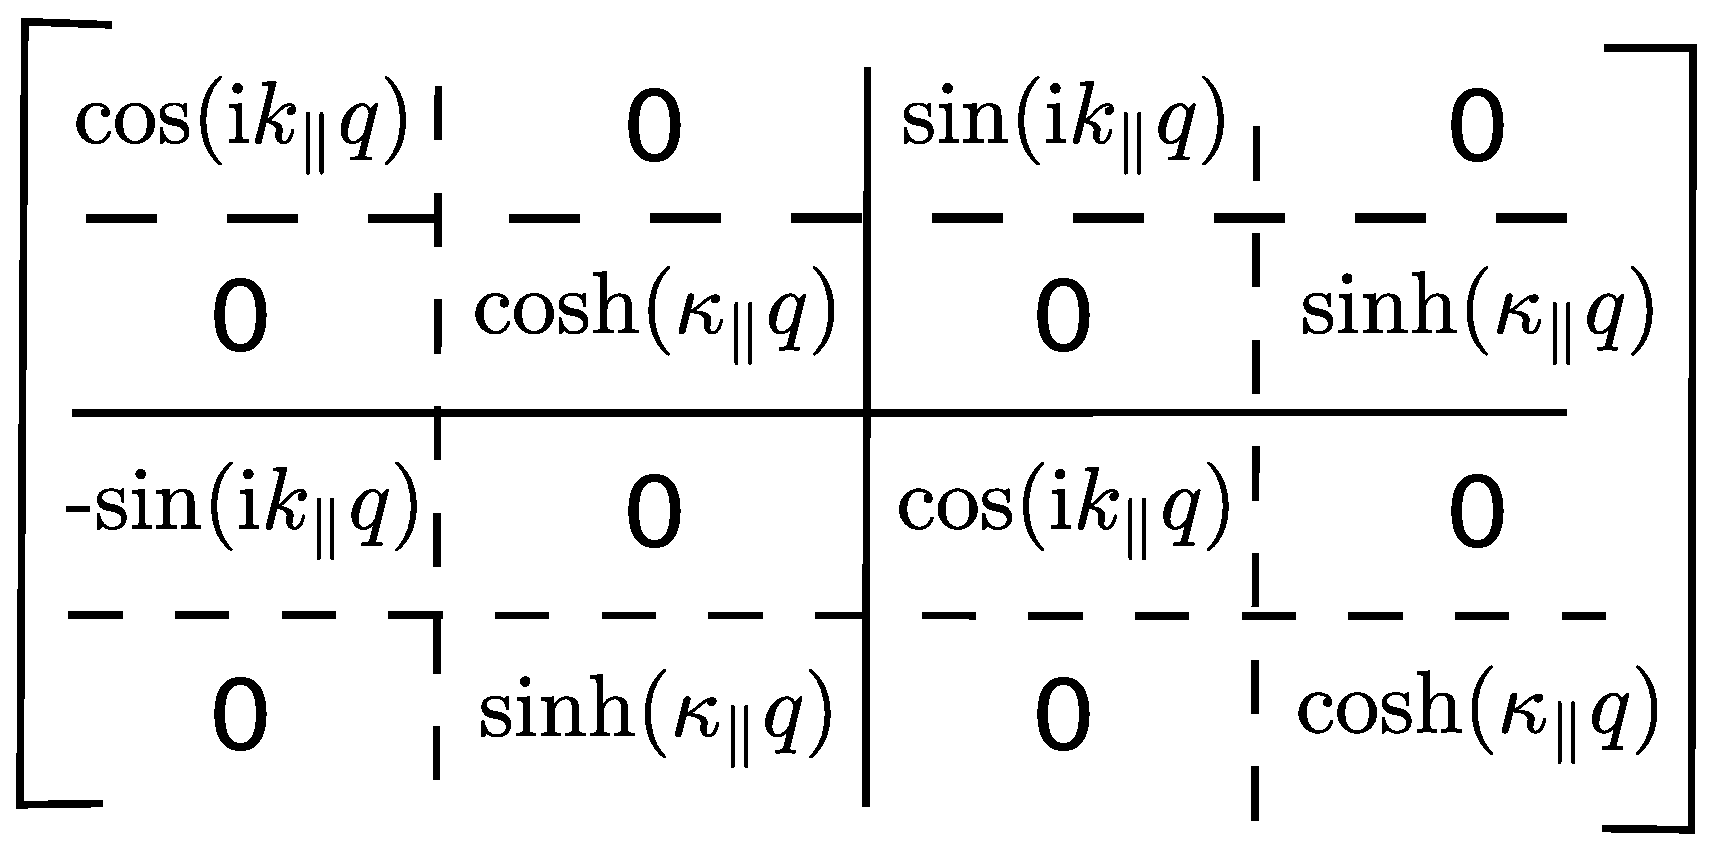
\includegraphics[height=3.9in]{chapters/Near-field_effects_in_wave_transport_through_in_disordered_waveguides/pictures/propagation_matrix_vector}}
%\begin{flushleft}(b)\end{flushleft}
\ (b)\ 
%\vskip -0.5cm
\scalebox{.5}{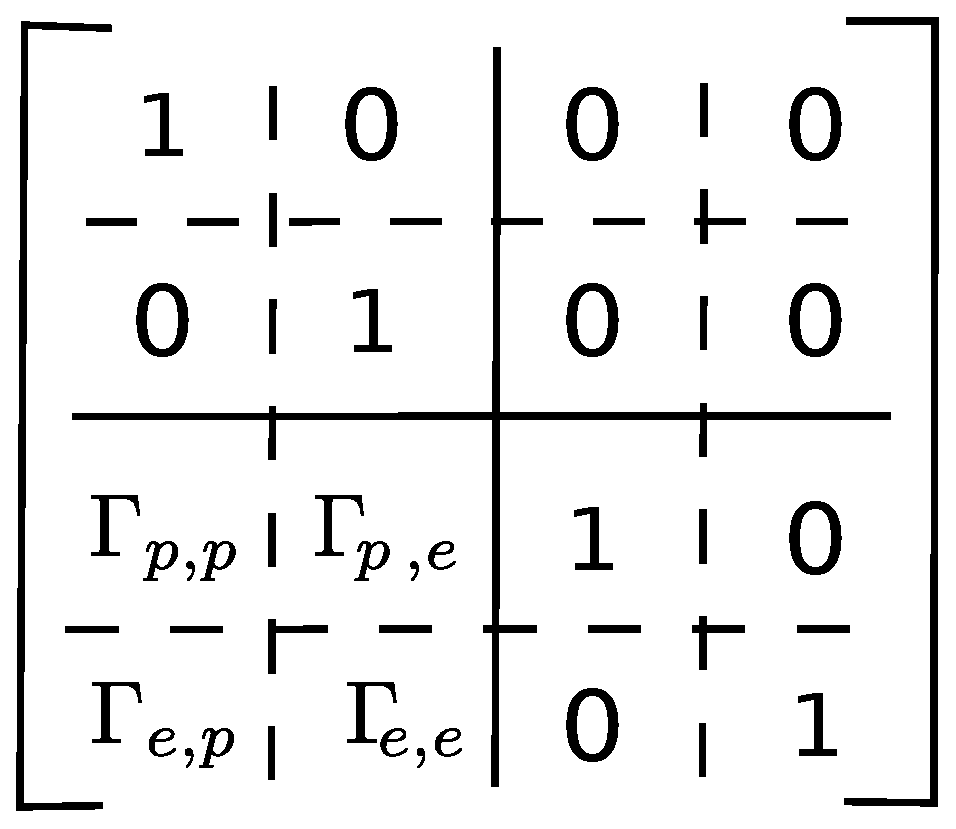
\includegraphics[height=3in]{chapters/Near-field_effects_in_wave_transport_through_in_disordered_waveguides/pictures/scattering_matrix_vector}}
}
\caption[(a) General form of empty waveguide transfer matrices for propagation of electric field $E$ and $E'$ over distance $\Delta z$ between scatterers.]{(a) General form of empty waveguide transfer matrices for propagation of electric field $E$ and $E'$ over distance $\Delta z$ between scatterers. (b) Scattering matrices, based on Eq.~\ref{eq:scattering_lines}, where $\Gamma_{nm}$ denotes non-zero terms which can be complex valued. Each matrix is separated into four $N_p+N_e $x$ N_p+N_e$ quadrants (long dashed lines), each containing information from propagating-to-propagating channels (upper left short-dashed subquadrants) as well as evanescent-to-evanescent (lower right short dashed subquadrants). }
\label{fig:tomsmatrices}
\end{figure}

%%%%%%%%%%%%%%%%%%%%%%%%%%%%%%%%%%%%%%%%%%%%%%%%%%%%%%%%%%%%%%%%%%%%%%%%%%%%%%
\subsection{Self-Embedding}
%%%%%%%%%%%%%%%%%%%%%%%%%%%%%%%%%%%%%%%%%%%%%%%%%%%%%%%%%%%%%%%%%%%%%%%%%%%%%%

%Due to the numerical instability which builds up in models of waveguides with many scatterers, 
The computation of the simple product of individual matrices is a straight-forward approach to field propagation but is not numerically stable over many multiplications, as the eigenvalues in the product become divergent~\cite{1968_Osedelec}. 
The self-embedding method derived in Ref.~\citenum{1999_yamilov_selfembed}
% (conceptually based on Ref.~\citenum{1976_Bellman_Wing_embedding}) 
is used to change the growth of error inherent in numerical matrix multiplication from exponential to linear. Deviation caused by diverging eigenvalues is corrected by renormalizing the products. This is critical as it allows the transfer matrix method to be used in the diffusive and localized regimes. 

Without self-embedding, exponential divergence of eigenvalues is commonly used to measure localization length. 
% what is the purpose of this previous statement?
Self-embedding technique increases the number of matrix multiplications that can be performed prior to the product matrix becoming unstable. Numerical instability grows linearly rather than exponentially, though computational time is increased compared to plain transfer matrix multiplication.  Here numerical stability is defined by conservation of flux; found by checking that the determinant of the product is unity.

With this numerical model we can determine the effect including evanescent channels on conductance. We show that single parameter scaling is obeyed; thus results extend to all other transport properties.


%%%%%%%%%%%%%%%%%%%%%%%%%%%%%%%%%%%%%%%%%%%%%%%%%%%%%%%%%%%%%%%%%%%%%%%%%%%%%%
\section{NUMERICAL SIMULATION RESULTS}
\label{sec:numericalResults}
%%%%%%%%%%%%%%%%%%%%%%%%%%%%%%%%%%%%%%%%%%%%%%%%%%%%%%%%%%%%%%%%%%%%%%%%%%%%%%
%
%outline:
%    a. for N_e=0, model matches theory
%    b. add N_e, P(g) changes.
%        i. dependence on alpha, density
%    c. with scaling, the N_e can be renormalized to N_e=0
%        i. recovers lack of dependence on alpha, density

To verify that the renormalizing effect of evanescent channels on transport mean free path does not affect single parameter scaling~\cite{1979_Anderson}, the ratio of average unitless conductance $ g \equiv \left\langle\sum_{a,b}^{N_p} |t_{a,b}|^2\right\rangle$ to variance of unitless conductance is computed by numerical simulation of quasi-1D waveguides. Once $g$ is known, single parameter scaling predicts all other transport properties are fixed (i.e., variance of conductance). Numerical results are compared to predictions from the non-linear sigma model~\cite{2000_Mirlin}, which assumes $N_p \rightarrow \infty$ and no evanescent channels. When no evanescent channels are present in our numerical model, the simulation results obey single parameter scaling and match non-linear sigma theory, c.f.~Fig.~\ref{fig:vargversusg}. No fitting parameters are used; the factor of $15/2$ is to account for the quasi-1D geometry of the waveguide. The use of self-embedding technique for renormalization of the transfer matrix method allows the numerical model to give results in the diffusive ($g>1$) and localized ($g<1$) regimes.

The variance of the conductance distribution decreases deeper into the localization regime; c.f.~Fig.~\ref{fig:vargversusg}. This is specific to the orthogonal universality class; in contrast, variance increases with~$L$ for symplectic and unitary models in the diffusive regime.

%Wiersma's question: why does variance decrease for increasing localization? Shouldn't we expect the distribution width to increase (longer tail)? As $g$ decreases (system becomes localized), fluctuations (distribution width) are expected to increase. The expectation is that fluctuations do not scale with $g$. Ratio of variance to average in both diffusive and localized regimes is what??

\begin{figure}
\vskip -0.5cm
\centerline{
\scalebox{.6}{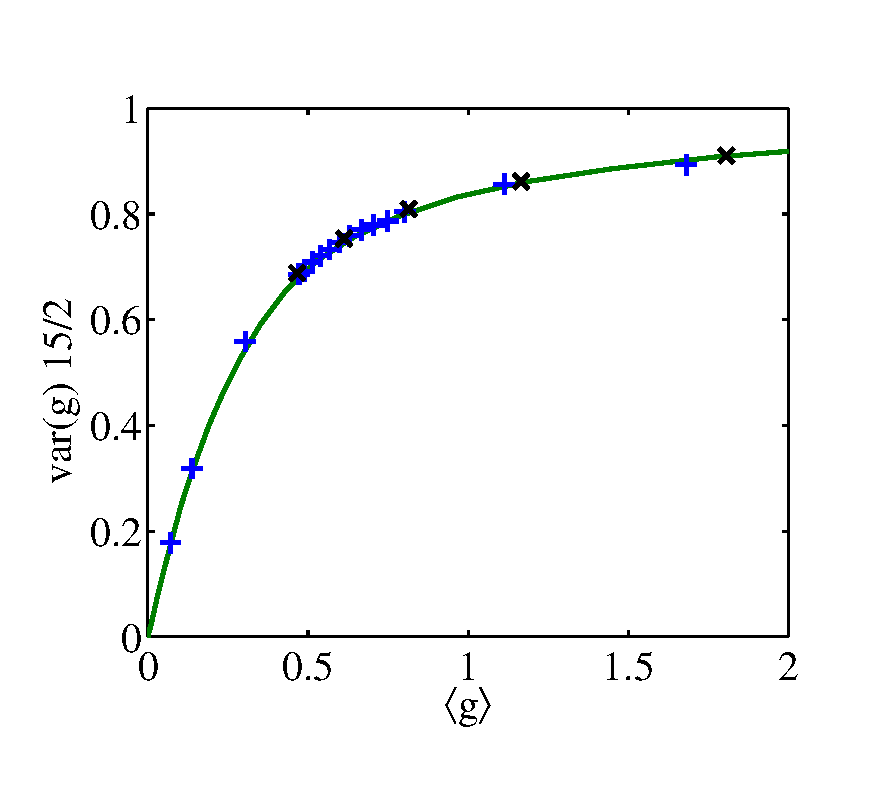
\includegraphics{chapters/Near-field_effects_in_wave_transport_through_in_disordered_waveguides/pictures/var_g_versus_g_no_closed_channels}}
}
\vskip -0.5cm
\caption[Variance of unitless conductance $g$ versus average $g$: comparison of quasi-1D numerical simulation results with non-linear sigma theory~\cite{2000_Mirlin} (solid green line) with no fitting parameters.]{Variance of unitless conductance $g$ versus average $g$: comparison of quasi-1D numerical simulation results with non-linear sigma theory~\cite{2000_Mirlin} (solid green line) with no fitting parameters. Waveguide results for with 10 (blue crosses) and 20 (black x) propagating channels and no evanescent channels when system length $L/\lambda$ is varied and $W/\lambda$ is constant. Very good agreement with the non-linear sigma model is found. Both numerical simulation and theory extend from diffusive ($g>1$) to localized ($g<1$) regime. The~$15/2$ coefficient for variance is due to waveguide geometry.}
% source of Mirlin's curve is Fig 6, page 349
% numerical data from 131.151.77.18/home/Q1D
\label{fig:vargversusg}
\end{figure}

When a finite number of evanescent channels are added, c.f.~Fig.~\ref{fig:vargversusgNCC}, the average conductance decreases. However, the ratio of average conductance to variance of conductance remains consistent with single parameter scaling %and with the theoretical prediction 
since variance also decreases. As more evanescent channels are included, the ratio monotonically decreases. %, while remaining on the curve which is based on no evanescent channels. 
Again, no fitting parameters are needed.
\begin{figure}
\vskip -0.5cm
\centerline{
\scalebox{.6}{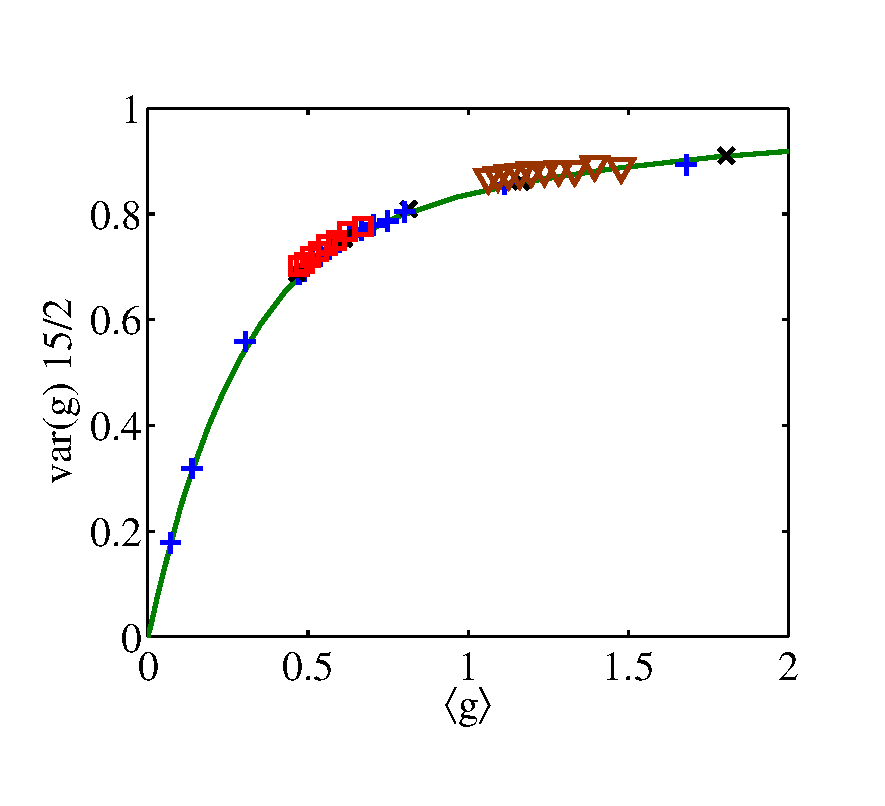
\includegraphics{chapters/Near-field_effects_in_wave_transport_through_in_disordered_waveguides/pictures/var_g_versus_g}}}
\vskip -0.5cm
\caption[Same data as in Fig.~\ref{fig:vargversusg} ($N_p=10$ blue crosses and $N_p=20$ black x for varying system length $L$).]{Same data as in Fig.~\ref{fig:vargversusg} ($N_p=10$ blue crosses and $N_p=20$ black x for varying system length $L$). Added here is $L/\lambda=100$, $N_p=10$ with 0 to 10 evanescent channels (brown triangles) and $L/\lambda=200$, $N_p=10$ with 0 to 8 evanescent channels (red squares). No fitting parameters used. Here the primary conclusion, that evanescent channels renormalize $\ell_{\rm tmfp}$ while retaining the property of single parameter scaling, is apparent. }
% numerical data from 131.151.77.18/home/Q1D
\label{fig:vargversusgNCC}
\end{figure}
There are two important observations from Fig.~\ref{fig:vargversusgNCC}. First, the average conductance decreases when more evanescent channels are present because $\ell_{\rm tmfp}$ is renormalized. More channels are available at each scatterer for incident waves to scatter into, and there is increased propagation between adjacent scatterers. Analytically, renormalization of $\ell$ is accounted for by the folding procedure. Thus DMPK theory is valid even though no evanescent channels are included: when compared to other theories or experiment, $\ell_{\rm tmfp}$ is a fitting parameter. Therefore the effect of evanescent channels is undetectable. The second observation is that because $\ell_{\rm tmfp}$ is renormalized, single parameter scaling remains valid whether or not evanescent channels are included. Numerical models that do not include evanescent channels give valid transport descriptions for passive media. 

%When including a finite number of evanescent channels, it has been shown here no upper limit exists on the necessary number of evanescent channels that make a significant contribution to transport even with a minimum scatterer separation distance of $\sqrt{\frac{W \ L}{M}}$. 

In real experimental systems, scatterers are finite sized. This means there is a finite number of evanescent channels needed to describe the wave around a scatterer. The closer any two scatterers are, the more evanescent channels that are needed to accurately describe wave propagation. %This can be accounted computationally for by placing scatterers in the medium the maximum distance apart for a given density. This suggests that saturation (a finite number of evanescent channels needed to describe the transport) is attainable given that the parameters fit a constraint~\cite{1990_Bagwell}: \textbf{[What is $m$ here?]}
%\begin{equation}
%\frac{m}{ \hbar^2 \kappa_n}\frac{\gamma}{W} <<1.
%\end{equation}
% This is an incorrectly copied formula from Bagwell PRB 1990. page 358. We would need to translate from electronic to photonic
% \frac{m}{ \hbar^2} = (1/2) \frac{\omega^2}{c^2}
% to get the condition
% \frac{\frac{\omega^2}{2 c^2} \frac{1}{\kappa_{\parallel n}} \frac{\alpha}{W} << 1
% 20080616, book 3 of Ben's notes
Delta-function scatterers would be resolved by an infinite number of evanescent channels, but saturation would occur for finite-sized scatterers.

\begin{figure}
\vskip -0.5cm
\centerline{
\scalebox{.5}{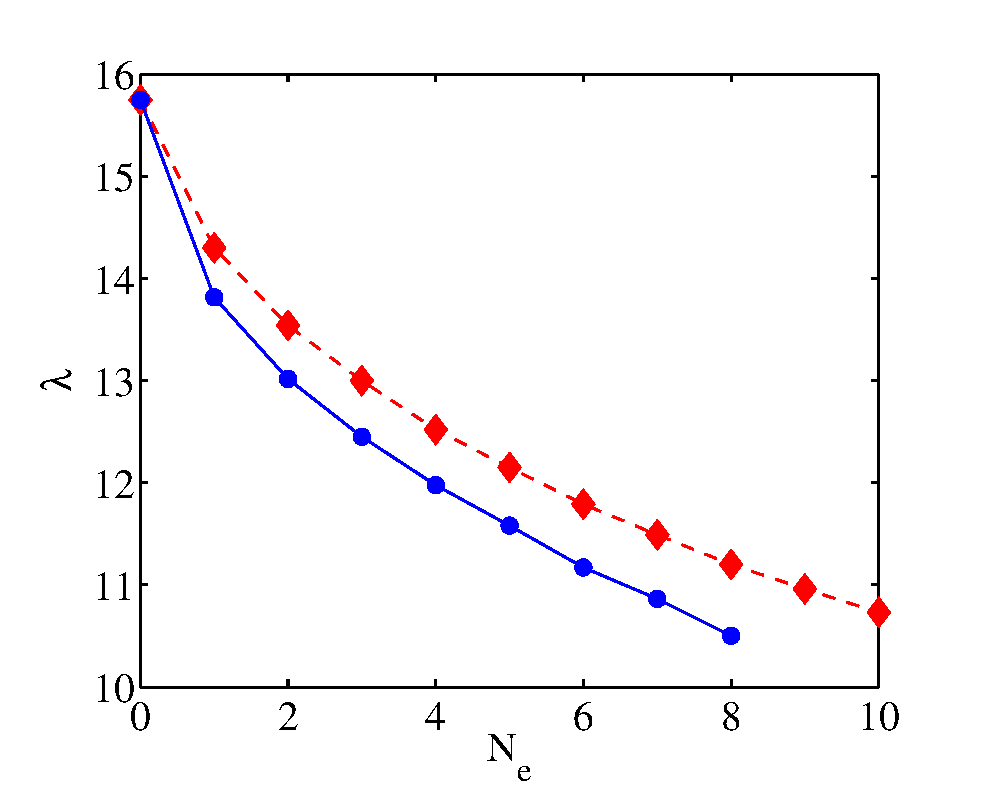
\includegraphics{chapters/Near-field_effects_in_wave_transport_through_in_disordered_waveguides/pictures/alpha1_W5_ltmfp_and_scat_versus_Nc_min_separation_05}}}
\vskip -0.2cm
\caption[Transport mean free path $\ell_{\rm tmfp}/\lambda$ (blue dots, solid line) renormalized as more evanescent channels ($N_e$) are included.]{Transport mean free path $\ell_{\rm tmfp}/\lambda$ (blue dots, solid line) renormalized as more evanescent channels ($N_e$) are included. % for $L/\lambda=200$, 10 propagating channels, $\alpha=1$ with minimum scatterer separation.
Red dashed line with diamonds is the scattering length defined by Eq.~\ref{eq:gb_lscat}. Both characteristic lengths are renormalized by inclusion of closed channels. No asymptotic value is apparent. 
}
\label{fig:lscat_ltmfp}
\end{figure}



Statements above concerning renormalization of $\ell_{\rm tmfp}$ above have only included the first two moments of conductance. To investigate whether all the moments are renormalized, we can find the entire distribution of conductance using the numerical model; c.f.~Fig.~\ref{fig:distgversusg}. When evanescent channels are included for a given waveguide geometry, the entire distribution changes (observed earlier as a change in both first and second moments). However, the system which includes evanescent channels has the same distribution as a longer waveguide with only propagating modes. Effectively, the presence of evanescent channels decreases $\ell_{\rm tmfp}$, which is equivalent to increasing system length $L$ since $g\propto~N_p\ell_{\rm tmfp}/L$. 
\begin{figure}
\vskip -0.5cm
\centerline{
\scalebox{.55}{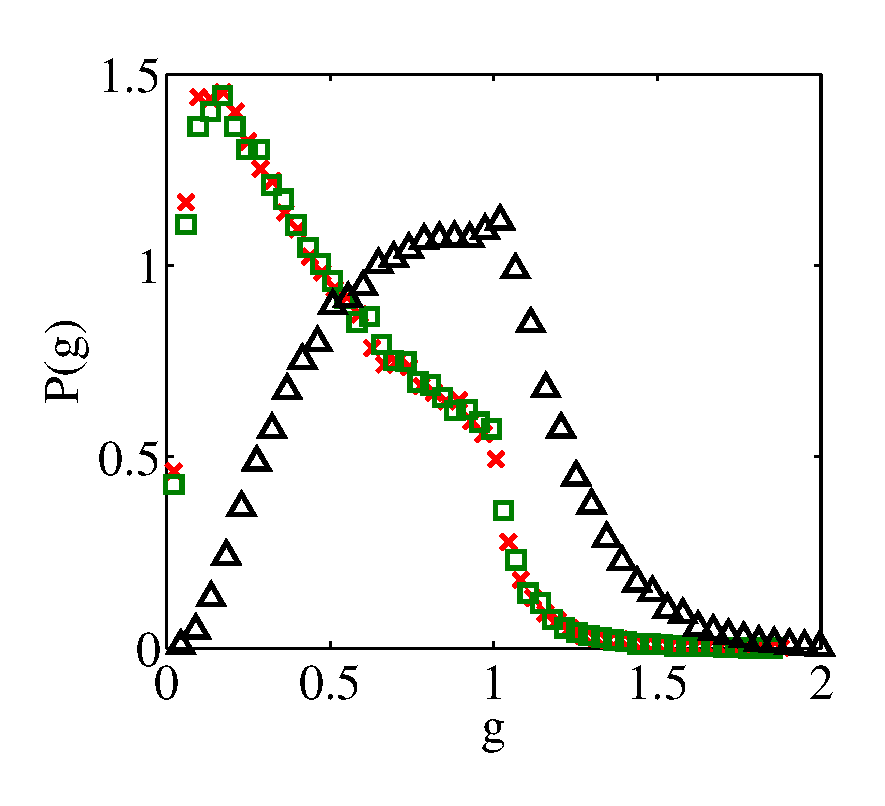
\includegraphics{chapters/Near-field_effects_in_wave_transport_through_in_disordered_waveguides/pictures/dist_g_vs_g_different_symbols_no_L600}}}
\vskip -0.5cm
\caption[Distribution of unitless conductance~$P(g)$ for three waveguides; each with 10 propagating channels.]{Distribution of unitless conductance~$P(g)$ for three waveguides; each with 10 propagating channels.  $P(g)$ from numerical simulation of waveguide system length $L/\lambda=200$ with no evanescent channels, black triangles is significantly distinct from $P(g)$ for same geometry and 8 evanescent channels (red x). However, the system with evanescent channels is equivalent to a longer system, $L/\lambda=300$, since $P(g)$ matches (green squares). The inclusion of evanescent channels renormalizes $\ell_{\rm tmfp}$ to be shorter, which is the equivalence of having a longer waveguide.}
% numerical data from 131.151.77.18/home/Q1D
\label{fig:distgversusg}
\end{figure}


%%%%%%%%%%%%%%%%%%%%%%%%%%%%%%%%%%%%%%%%%%%%%%%%%%%%%%%%%%%%%%%%%%%%%%%%%%%%%%
\section{CONCLUSION}
%%%%%%%%%%%%%%%%%%%%%%%%%%%%%%%%%%%%%%%%%%%%%%%%%%%%%%%%%%%%%%%%%%%%%%%%%%%%%%

The characteristic length for transport properties in random media with multiple scattering is $\ell_{\rm tmfp}$. Using analytical and computational analysis we have shown the renormalization of $\ell_{\rm tmfp}$ due to evanescent channels. For the analytical portion, the transfer matrix folding technique used by Bagwell and coworkers for single scatterers extends to multiple scatterers, which include density information. Thus $\ell_{\rm tmfp}$ is renormalized due to evanescent channels. 

Using a numerical transfer-matrix model of quasi-1D waveguides with densely packed, randomly-placed scatterers the effect of evanescent channels on conductivity was simulated. The number of matrices multiplied is limited by numerical accuracy, and has been extended using self-embedding technique~\cite{1999_yamilov_selfembed}. Transfer matrices can include a finite number propagating and evanescent channels. The number of evanescent channels was varied and single parameter scaling remained valid. Comparison with theoretical predictions agreed with no fitting parameters. However, the first and second moments of conductance decreased as more  evanescent channels were added. This can be attributed to the shorter $\ell_{\rm tmfp}$. 

The distribution of conductance changes when the number of evanescent channels is varied but is equivalent to a system with no evanescent channels and longer $L$ or a shorter $\ell_{\rm tmfp}$. The renormalization of $\ell_{\rm tmfp}$ due to evanescent channels explains how DMPK theory, in which $\ell_{\rm tmfp}$ is used as a fitting parameter, can agree with experimental measurements which necessarily include evanescent channels.

The results of our \textit{ab initio} numerical model are be explained by the folding procedure which analytically reduces the rank of transfer matrices to propagating channels only. We demonstrated renormalization applies to multiple scatterers, thus including interaction between scatterers, by finding $\ell_{\rm tmfp}$ as a function of the number of evanescent channels. Folding a single scatterer matrix renormalizes $\ell$, but inclusion of multiple scatterers is necessary to renormalize $\ell_{\rm tmfp}$. Since single parameter scaling is valid and average conductance is $g \propto N \ell_{\rm tmfp}/L$, then the entire distribution of conductance is reshaped. 

These effect of evanescent channels on transport properties is expected to be important in media with gain. We have shown using numerical simulations that evanescent channels renormalize $\ell_{\rm tmfp}$, which includes interaction between scatterers. 

% \newpage
%
% \begin{appendices}
% 
%   \renewcommand{\theequation}{A-\arabic{equation}}
%   % redefine the command that creates the equation no.
%   \setcounter{equation}{0}  % reset counter 
% 
% \include{appendix_derivation_single_scatterer_transfer_matrix}
% 
%   \renewcommand{\theequation}{B-\arabic{equation}}
%   % redefine the command that creates the equation no.
%   \setcounter{equation}{0}  % reset counter 
% 
% \include{appendix_derivation_folding_one_scattering_matrix}
% 
%   \renewcommand{\theequation}{C-\arabic{equation}}
%   % redefine the command that creates the equation no.
%   \setcounter{equation}{0}  % reset counter 
% 
% \include{appendix_derivation_folding_two_scatterers}
% 
%   \renewcommand{\theequation}{D-\arabic{equation}}
%   % redefine the command that creates the equation no.
%   \setcounter{equation}{0}  % reset counter 
% 
% \include{appendix_derivation_folding_two_scatterers_matrices}
% \newpage
% \end{appendices}
% 
% \bibliographystyle{apsrevM}
% %\bibliographystyle{unsrt} % order the citations according to when they show up in the paper
% \bibliography{../../Bibliography/latex_bibliography}

% also need to cite 1991_Mello_Tomsovic

%useful sites for latex formatting
%  http://en.wikibooks.org/wiki/LaTeX/Mathematics
%  http://www.tex.ac.uk/cgi-bin/texfaq2html?label=appendix
%conventions:
%  Fig.~\ref{fig:
%  Eq.~\ref{
%  Ref.~\cite{
%\end{document}
%eof

\label{paper:3_end}

\PaperManuscript{4}{Anderson Localization as position-dependent diffusion in disordered waveguides}
% Phys. Rev. B 82, 024205 (2010) doi:10.1103/PhysRevB.82.024205
% /svn/research/Project_Quasi1D_Transport/2010_Dofz_manuscript/quasi1d_dofz_prb.tex
\setcounter{section}{0}
\setcounter{figure}{0}
\setcounter{table}{0}
\label{paper:4_start}
% %\documentclass[prb,preprint,showpacs,amsmath,amssymb          ]{revtex4}
% \documentclass[prb,         showpacs,amsmath,amssymb,twocolumn]{revtex4}
% 
% % Some other (several out of many) possibilities
% %\documentclass[preprint,aps]{revtex4}
% %\documentclass[preprint,aps,draft]{revtex4}
% %\documentclass[prb]{revtex4}% Physical Review B
% %\usepackage{wasysym}
% %\usepackage{bm}
% %\usepackage[usenames]{color}
% %\renewcommand\arraystretch{2.2}
% 
% \usepackage{dcolumn}
% \usepackage{verbatim} % multi-line comments
% \usepackage{graphicx}
% \usepackage{epsfig}
% \usepackage{hyperref} % hyperlinked references and figures
% %\usepackage{color}
% 
% \begin{document}
%\newcommand{\boldnabla}{\mbox{\boldmath$\nabla$}}

\chapter{Anderson localization as position-dependent diffusion in disordered waveguides}
\label{chap:Dz_absorb}
\label{paper:4_start}

% \author{Ben Payne$^1$, Alexey Yamilov$^1$\footnote{Electronic~address:~yamilov@mst.edu} and Sergey E. Skipetrov$^2$\footnote{Electronic~address:~Sergey.Skipetrov@grenoble.cnrs.fr}}
\begin{center}
Ben Payne$^1$, Alexey Yamilov$^1$, and Sergey E. Skipetrov$^2$
\end{center}

\ \\
\begin{center}
\textit{$^1$Department of Physics, Missouri University of Science \& Technology,\\ Rolla, MO 65409\\
$^2$Universit\'{e} Joseph Fourier, Laboratoire de Physique et Mod\'{e}lisation des Milieux Condens\'{e}s, CNRS, 25 rue des Martyrs, BP 166, 38042 Grenoble, France}\end{center}

\ \\
% \affiliation{$^1$Department of Physics, Missouri University of Science \& Technology, Rolla, MO 65409\\
% $^2$Universit\'{e} Joseph Fourier, Laboratoire de Physique et Mod\'{e}lisation des Milieux Condens\'{e}s, CNRS, 25 rue des Martyrs, BP 166, 38042 Grenoble, France}
% 
% \date{\today}
% 
% \begin{abstract}
\addcontentsline{toc}{section}{ABSTRACT}
\begin{center}\textbf{ABSTRACT\footnote{Published in Physical Review B \textbf{82} 024205 (2010).}}        \end{center}

We show that the recently developed self-consistent theory of Anderson localization with a position-dependent diffusion coefficient is in quantitative agreement with the supersymmetry approach up to terms of the order of $1/g_0^2$ (with $g_0$ the dimensionless conductance in the absence of interference effects) and with  large-scale {\it ab-initio} simulations of the classical wave transport in disordered waveguides, at least for $g_0 \gtrsim 0.5$. In the latter case, agreement is found  even in the presence of absorption. Our numerical results confirm that in open disordered media,  the onset of  Anderson localization can be viewed as position-dependent diffusion.
% \end{abstract}
% 
% % 42.25.Dd - Wave propagation in random media
% % 72.15.Rn - Localization effects (Anderson or weak localization)
% \pacs{42.25.Dd, 72.15.Rn}
% 
% \maketitle

%=====================================================================================================================

\section{INTRODUCTION}


Anderson localization is a paradigm in condensed matter physics~\cite{1958_Anderson}. It consists in a blockade of the diffusive electronic transport in disordered metals due to interferences of multiply scattered de Broglie waves at low temperatures and at a sufficiently strong disorder. This phenomenon is not unique to electrons but can manifest itself for any wave in the presence of disorder, in particular for classical waves, such as light and sound~\cite{1984_John_prl}, and, as shown more recently, for matter waves~\cite{2008_Billy}. Although the absence of decoherence and interactions~\cite{2007_Akkermans_book} for classical waves is appealing in the context of the original idea of Anderson, serious complications appear due to absorption of a part of the wave energy by the disordered medium~\cite{1991_Genack}.
Extracting clear signatures of Anderson localization from experimental signals that are strongly affected by --- often a poorly controlled -- absorption was the key to success in recent experiments with microwaves~\cite{2000_chabanov_nature,2003_Genack}, light~\cite{2006_Maret_PRL} and ultrasound~\cite{2008_van_Tiggelen_Nature}.

Classical waves offer a unique possibility of performing angle-, space-, time- or frequency-resolved measurements with excellent resolution, the possibility that was not available in the realm of electronic transport. In a wider perspective, they also allow a controlled study of the interplay between disorder and interactions, as illustrated by the recent work on disordered photonic lattices~\cite{2007_Segev}.
Interpretation of measurements requires a theory that would be able to describe not only the genuine interferences taking place in the bulk of a large sample but also the modification of these interferences in a sample of particular shape, of finite size, and with some precise conditions at the boundaries. Such a theory has been recently developed~\cite{2000_van_Tiggelen,2004_Skipetrov,2006_Skipetrov_dynamics,2008_Cherroret} based on the self-consistent (SC) theory of Vollhardt and W\"{o}lfle~\cite{1980_Vollhardt_Wolfle}. The new ingredient is the position dependence of the renormalized diffusion coefficient $D(\mathbf{r})$ that accounts for a stronger impact of interference effects in the bulk of the disordered sample as compared to the regions adjacent to boundaries. This position dependence is crucial in open disordered media~\cite{2009_Cherroret}. $D(\mathbf{r})$ also appears in the supersymmetry approach to wave transport~\cite{2008_Tian}, which confirms that this concept goes beyond a particular technique (diagrammatic or supersymmetry methods) used in the calculations.

The SC theory with a position-dependent diffusion coefficient was successfully applied to analyze microwave~\cite{2004_Skipetrov} and ultrasonic~\cite{2008_van_Tiggelen_Nature} experiments. The predictions of the theory~\cite{2006_Skipetrov_dynamics} are also in qualitative agreement with optical experiments of St\"{o}rzer \textit{et al.}~\cite{2006_Maret_PRL}. However, it remains unclear whether the position dependence of $D$ is just a (useful) mathematical concept or if it is a genuine physical reality. In addition, the extent to which predictions of SC theory are quantitatively correct is not known. Obviously, the last issue is particularly important once comparison with experiments is attempted.

In the present paper we compare the predictions of SC theory of localization with the known results obtained previously using the supersymmetry method~\cite{2000_Mirlin} and with the results of extensive \textit{ab-initio} numerical simulations of wave transport in two-dimensional (2D) disordered waveguides. We demonstrate, first, that the position-dependent diffusion is a physical reality and, second, that SC theory agrees with the supersymmetry approach up to terms of the order of $1/g_0^2$ (with with $g_0$ the dimensionless conductance in the absence of interference effects) and with numerical simulation at least for $g_0 \gtrsim 0.5$. In the latter case, the agreement is found even in the presence of absorption.

%=====================================================================================================================
\section{SELF-CONSISTENT THEORY OF LOCALIZATION}
\label{sec:sctheory}

We consider a scalar, monochromatic wave $u(\mathbf{r})e^{-i \omega t}$ propagating in a 2D volume-disordered waveguide of width $w$ and length $L \gg w$. The wave field $u(\mathbf{r})$ obeys the 2D Helmholtz equation:
\begin{equation}
\left\{\nabla^2 + k^2\left[1 + i \epsilon_a + \delta\epsilon(\mathbf{r}) \right]\right\} u(\mathbf{r}) = 0.
\label{eq:helmholtz}
\end{equation}
Here $k=\omega/c$ is the wavenumber, $c$ is the speed of the wave in the free space, $\epsilon_a$ is the imaginary part of the dielectric constant accounting for the (spatially uniform) absorption in the medium, and $\delta\epsilon(\mathbf{r})$ is the randomly fluctuating part of the dielectric constant.
Assuming that $\delta\epsilon(\mathbf{r})$ is a Gaussian random field with a short correlation length, it is easy to show that the disorder-averaged Green's function of Eq.~(\ref{eq:helmholtz}), $\langle G(\mathbf{r}, \mathbf{r}') \rangle$, decays exponentially with the distance $|\mathbf{r}-\mathbf{r}'|$
\cite{2007_Akkermans_book}. The characteristic length of this decay defines the mean free path $\ell$. In this paper we consider quasi-1D waveguides defined by the condition $w \lesssim \ell \ll L$. The intensity Green's function of Eq.~(\ref{eq:helmholtz}), $C(\mathbf{r}, \mathbf{r}') = (4\pi/c)
\langle \left| G(\mathbf{r}, \mathbf{r}') \right|^2 \rangle$, obeys self-consistent equations that can be derived following the approach of Ref.~\citenum{2008_Cherroret}. In a quasi-1D waveguide, all position-dependent quantities become functions of the longitudinal coordinate $z$ only and the stationary SC equations can be written in a dimensionless form:
\begin{eqnarray}
&&\left[\beta^2 - \frac{\partial}{\partial \zeta} d(\zeta)
 \frac{\partial}{\partial \zeta} \right] {\hat C}(\zeta,\zeta')
= \delta(\zeta-\zeta'),
\label{eq:sceq1}
\\
&&\frac{1}{d(\zeta)} =  1+\frac{2}{{\tilde g}_0}
{\hat C}(\zeta,\zeta).
\label{eq:sceq2}
\end{eqnarray}
Here ${\hat C}(\zeta,\zeta') = (w D_0/L)C(\mathbf{r},\mathbf{r}')$,
$D_0 = c\ell/2$ is the Boltzmann diffusion coefficient, $\zeta = z/L$ is the dimensionless coordinate, $d(\zeta) = D(z)/D_0$ is the normalized position-dependent diffusion coefficient, $\beta = L/L_a$ is the absorption coefficient (with $L_a = \sqrt{\ell \ell_a/2}$ and $\ell_a = 1/k\epsilon_a$ the macro- and microscopic absorption lengths, respectively), and ${\tilde g}_0 = (\pi/2)N \ell/L$ with $N = kw/\pi$ the number of the transverse modes in the waveguide. These equations should be solved with the following boundary conditions:
\begin{eqnarray}
{\hat C}(\zeta,\zeta^{\prime}) \mp
\frac{z_0}{L} d(\zeta) \frac{\partial}{\partial \zeta}
{\hat C}(\zeta,\zeta^{\prime}) = 0
\label{eq:bc}
\end{eqnarray}
at $\zeta = 0$ and $\zeta = 1$. Similarly to the 3D case~\cite{2008_Cherroret}, these conditions follow from the requirement of vanishing incoming diffuse flux at the open boundaries of the sample. $z_0$ is the so-called extrapolation length equal to $(\pi/4)\ell$ in the absence of internal reflections at the sample surfaces~\cite{1999_van_Rossum}. We will use $z_0 = (\pi/4) \ell$ throughout this paper. When Eqs.\ (\ref{eq:sceq1}--\ref{eq:bc}) are solved in the diffuse regime ${\tilde g}_0 \gg 1$, the dimensionless conductance of the waveguide is found to be $g_0 = (\pi/2)N \ell/(L + 2 z_0)$ ~\cite{1999_van_Rossum,1997_Beenakker} which is close to ${\tilde g}_0$ for $z_0 \ll L$.

In the absence of absorption ($\beta = 0$) we can simplify Eq.~(\ref{eq:sceq1}) by introducing $\tau = F(\zeta) = \int_0^{\zeta} d\zeta_1/d(\zeta_1)$:
\begin{eqnarray}
-\frac{\partial^2}{\partial \tau^2} {\hat C}(\tau, \tau^{\prime})
= \delta(\tau-\tau^{\prime}),
\label{eq:sceq3}
\end{eqnarray}
with the boundary conditions (\ref{eq:bc}) becoming
\begin{eqnarray}
{\hat C}(\tau, \tau^{\prime}) \mp
\tau_0 \frac{\partial}{\partial \tau}
{\hat C}(\tau, \tau^{\prime}) = 0,
\label{eq:bc3}
\end{eqnarray}
and $\tau^{\prime} = F(\zeta^{\prime})$, $\tau_0 = z_0/L$. Equations (\ref{eq:sceq3}) and (\ref{eq:bc3}) are readily solved:
\begin{eqnarray}
{\hat C}(\tau, \tau^{\prime}) =
\frac{(\tau_< + \tau_0)(\tau_{\mathrm{max}} + \tau_0 - \tau_>)}{\tau_{\mathrm{max}} + 2 \tau_0},
\label{eq:sol}
\end{eqnarray}
where $\tau_< = \min(\tau, \tau^{\prime})$, $\tau_> = \max(\tau, \tau^{\prime})$ and $\tau_{\mathrm{max}} = F(1)$.  We now substitute this solution into Eq.~(\ref{eq:sceq2}) to obtain
\begin{eqnarray}
\frac{1}{d(\tau)} \equiv \frac{d \tau}{d\zeta} =
1 + \frac{2}{\tilde g}_0 \times \frac{(\tau + \tau_0)(\tau_{\mathrm{max}} + \tau_0 - \tau)}{\tau_{\mathrm{max}} + 2 \tau_0}.
\label{eq:dtdz}
\end{eqnarray}
This differential equation can be integrated to find $\tau$ as a function of $\zeta$. Using $d(\zeta) = (d\tau/d\zeta)^{-1}$ we finally find
\begin{eqnarray}
d(\zeta) &=& \left\{ {\tilde g}_0 \sqrt{p} \cosh(\sqrt{p} \zeta/{\tilde g}_0) \right.
\nonumber \\
&-& \left. [{\tilde g}_0 + \tau_0(1 - p)] \sinh(\sqrt{p} \zeta/{\tilde g}_0) \right\}^2
\nonumber \\
&\times& \left\{ p [({\tilde g}_0 + \tau_0)^2 - \tau_0^2 p]
\right\}^{-1},
\label{eq:dzsol}
\end{eqnarray}
where $p$ is the solution of a transcendental equation
\begin{eqnarray}
\frac{2 {\tilde g}_0}{\sqrt{p}}
\mathrm{arctanh} \left\{ \frac{1}{\sqrt{p}}
\left[ 1 - \frac{\tau_0}{{\tilde g}_0} \left(p - 1 \right) \right] \right\} = 1.
\label{eq:p}
\end{eqnarray}
Solving the last equation numerically and substituting the result into Eq.~(\ref{eq:dzsol}) we can find the profile $d(\zeta)$ at any ${\tilde g}_0$ and $\tau_0 = z_0/L$. In contrast,
for $\beta > 0$ Eqs.\ (\ref{eq:sceq1}--\ref{eq:bc}) do not admit analytic solution and we solve them by iteration: we start with $D(z) = D_0$, solve Eq.~(\ref{eq:sceq1}) numerically with the boundary conditions (\ref{eq:bc}) and then find the new $D(z)$ from Eq.~(\ref{eq:sceq2}). This procedure is then repeated until it converges to a solution. In typical cases considered in this paper the convergence is achieved after 10--20 iterations.

The simplest object that Eqs.\ (\ref{eq:sol}--\ref{eq:dzsol}) allows us to study is the average conductance of the waveguide $\langle g \rangle$. Indeed, the average transmission coefficient of the waveguide is found as
\begin{eqnarray}
T &=& -D(L) \left. \frac{dC(z, z^{\prime}=\ell)}{dz} \right|_{z=L}
\nonumber \\
&=& - \frac{1}{w} \times \left.
\frac{d{\hat C}(\tau, \tau_{\ell})}{d\tau}
\right|_{\tau = \tau_{\mathrm{max}}}
\nonumber \\
&=& \frac{1}{w} \times \frac{\tau_{\ell} + \tau_0}{\tau_{\mathrm{max}} + 2 \tau_0},
\label{eq:t}
\end{eqnarray}
where $\tau_{\ell} = F(\ell/L)$.
For the waveguide we have $\langle g \rangle \propto T$. A ratio that emphasizes the impact of localization effects is $\langle g \rangle/g_0 = T/T_0$, where $T_0$ is the average transmission coefficient found in the absence of localization effects (i.e., for $d \equiv 1$): $T_0 = (\ell + z_0)/w(L + 2 z_0)$. We find
\begin{eqnarray}
\frac{\langle g \rangle}{g_0} =
\frac{L + 2 z_0}{\ell + z_0}
(\tau_{\ell} + \tau_0)
\frac{p - 1}{2 {\tilde g}_0}.
\label{eq:goverg0}
\end{eqnarray}

Simple analytic results follow for $z_0 = 0$, when $g_0 = {\tilde g}_0$. Equation (\ref{eq:dzsol}) yields
\begin{eqnarray}
d(\zeta) &=& \left[ \frac{\sinh(\sqrt{p} \zeta/g_0)}{\sqrt{p}} - \cosh(\sqrt{p} \zeta/g_0) \right]^2
\label{eq:dzsol2}
\end{eqnarray}
and we find
\begin{eqnarray}
\tau_{\ell} &=& \frac{g_0}{\sqrt{p}\; \mathrm{cotanh}
(\sqrt{p} \ell/L g_0) -1}.
\label{eq:tauell}
\end{eqnarray}
In the weak localization regime $g_0 \gg 1$ the solution $p$ of Eq.~(\ref{eq:p}) can be found as a series expansion in powers of $1/g_0$:
$p = 2 g_0 + 1/3 + 2/45 g_0 - 17/540 g_0^2 + \ldots$.
If we keep only the first term $p = 2 g_0$, substitute it into Eq.~(\ref{eq:dzsol2}) and expand in powers of $1/g_0 \ll 1$, we obtain
$D(z) \simeq D_0 [ 1 - (2/g_0) (z/L)(1-z/L)]$.
Keeping terms up to $1/g_0^2$ in the expression for $p$ and substituting it into Eqs.\ (\ref{eq:tauell}) and (\ref{eq:goverg0}), expanding the result in powers of $1/g_0$ and then taking the limit of $L/\ell \rightarrow \infty$, we obtain
\begin{eqnarray}
\frac{\langle g \rangle}{g_0} \simeq
1 - \frac{1}{3 g_0} + \frac{1}{45 g_0^2} + \frac{2}{945 g_0^3} + \ldots.
\label{eq:goverg01}
\end{eqnarray}
This result coincides {\em exactly} with Eq.~(6.26) of Ref.~\cite{2000_Mirlin} obtained by Mirlin using supersymmetry approach, except for a factor of 2 due to two independent spin states of electrons in Ref.~\cite{2000_Mirlin}. We therefore proved the exact equivalence between SC theory and the supersymmetry approach for the calculation of the average conductance $\langle g \rangle$ up to terms of the order of $1/g_0^2$.

Deep in the localized regime $g_0 \ll 1$ and Eq.~(\ref{eq:p}) can be solved approximately to yield
$p = 1 + 4 \exp(-1/g_0)$ (always for $z_0 = 0$ and hence for $g_0 = {\tilde g}_0$).
If we substitute this $p$ into Eq.~(\ref{eq:dzsol2}), we obtain
$D(z) \simeq D_0 \{ \exp(-z/\xi) + \exp[-(L-z)/\xi] \}^2$, where $\xi = g_0 L$ is the localization length.
Equations (\ref{eq:tauell}) and (\ref{eq:goverg0}) then yield
\begin{eqnarray}
\frac{\langle g \rangle}{g_0} \simeq
\frac{2}{g_0} \exp\left(-\frac{1}{g_0} \right),
\label{eq:goverg02}
\end{eqnarray}
where we made use of the fact that $L/\ell \gg 1$ and $N \gg 1$.
In contrast to Eq.~(\ref{eq:goverg01}), this result differs from the one obtained using the supersymmetry approach [see Eq.~(6.29) of Ref.~\cite{2000_Mirlin}]. Even though the exponential decay of conductance with $1/g_0 = L/\xi$ --- expected in the localized regime --- is reproduced correctly, both the rate of this decay and the pre-exponential factor are different. We thus conclude that SC theory does not provide quantitatively correct description of stationary wave transport in disordered waveguides in the localized regime.

It is worthwhile to note that the breakdown of SC theory for $g_0 \ll 1$ is not surprising and could be expected from previous results. Indeed, it has already been noted that for the time-dependent transmission, SC theory does not apply after the Heisenberg time $t_H$~\cite{2004_Skipetrov}. The stationary transmission coefficient $T$ of Eq.~(\ref{eq:t}) is an integral of the time-dependent transmission $T(t)$: $T = \int_0^{\infty} dt\; T(t)$, with the peak of $T(t)$ around the Thouless time $t_D = L^2/\pi^2 D_0$~\cite{2004_Skipetrov}. When $g_0 \sim t_H/t_D \gg 1$, the integral is dominated by $t < t_H$ where SC theory applies. The integration thus yields the correct $T$. However, when $g_0 \ll 1$, $t_H$ is smaller than $t_D$ and the main part of pulse energy arrives at $t > t_H$. Such long times are beyond the reach of SC theory, hence its breakdown for small $g_0$.

%=====================================================================================================================
\section{NUMERICAL MODEL}
\label{sec:numerical}

To test the predictions of the SC model discussed in the previous section we solve Eq.~(\ref{eq:helmholtz}) numerically using the method of transfer matrices defined in the basis of the transverse modes of the empty waveguide~\cite{2007_Froufe-Perez_PRE,2010_Payne_closed}. To this end, we represent $\delta \epsilon(\mathbf{r})$ as a collection of $M$ randomly positioned ``screens'' perpendicular to the axis $z$ of the waveguide and characterized by random functions $f_{\nu}(y) = \sum_{n=1}^N \chi_n(y)\chi_n(y_\nu)$:
\begin{equation}
\delta\epsilon(\mathbf{r}) = \alpha\sum\limits_{\nu=1}^M \delta(z - z_\nu)f_\nu(y).
\label{de}
\end{equation}
Here $\chi_n(y) = (2/w)^{1/2}\sin(\pi ny/w)$ are the transverse modes of the waveguide and $y_\nu$ are chosen at random within the interval $(0, w)$. $z_\nu$ represent random positions of the screens, whereas $\alpha$ measures their scattering strength. Absorption can be included in the model by making $\alpha$ complex.

In the limit $N\rightarrow\infty$, $f_\nu(y)$ becomes a delta-function $\delta\left(y-y_\nu\right)$, mimicking a point-like scatterer. By the choice of $f_\nu(y)$ in Eq.~(\ref{de}) we narrowed the basis to $N$ right- and $N$ left-propagating modes with real values of the longitudinal component of the wavevector. Such modes are often termed ``open channels'' in the literature~\cite{2007_Froufe-Perez_PRE}. Hence, the total transfer matrix of the system is a product of $M$ pairs of $2N\times 2N$ scattering matrices corresponding to the random screens positioned at $z_{\nu}$ and the free space in between them, respectively~\cite{2010_Payne_closed}. Because the numerical computation of products of a large number of transfer matrices ($\sim 10^2$--$10^5$ for the results in this paper) is intrinsically unstable, we implement a self-embedding procedure~\cite{1999_yamilov_selfembed} which limits the errors in flux conservation to less than $10^{-10}$ in all cases. The system is excited by illuminating the waveguide with $N$ unit fluxes (one in each right propagating mode) and the wave field $u(\mathbf{r})$ is computed~\cite{1999_yamilov_selfembed,2010_Payne_closed} for a given realization of disorder [see the inset of Fig.~\ref{fig1}(a)]. To compute statistical averages, ensembles of no fewer than $10^7$ realizations are used.

%---------------------------------------------------------------------------------------------------------------------
\begin{figure*}
%\vskip -0.5in
%\centering{\includegraphics[height=6.5in,angle=-90]{fig1}}
%\vskip -1.75in
\vskip -0.3in
\centering{\includegraphics[width=4.5in,angle=-90]{chapters/Anderson_Localization_as_position-dependent_diffusion_in_disordered_waveguides__Phys_Rev_B/pictures/fig1}}
\vskip -1.9in
\caption[The average (a) and the variance (b) of the conductance $g$ of disordered waveguides supporting $N=10$ (circles) 
and $N=20$ (squares) modes are shown versus the inverse of $g_0$.]{\label{fig1}
The average (a) and the variance (b) of the conductance $g$ of disordered waveguides supporting $N=10$ (circles) 
and $N=20$ (squares) modes are shown versus the inverse of $g_0$. The solid lines marked as SUSY are fits using 
Eq.~(6.23) of Ref.~\cite{2000_Mirlin}, derived using the supersymmetry approach, with $\ell = 15.7 \lambda$ as the only 
fit parameter. The solid line marked as SC in (a) is obtained using the self-consistent theory [Eq.~(\ref{eq:goverg0})]. Inset in (a): for a given realization of disorder, wave ``trajectories'' found by connecting local Poynting vectors are superimposed on the distribution of intensity $|u(\mathbf{r})|^2$ in a disordered waveguide with $w=10.25\lambda$ and $L=50\lambda$. Only trajectories that traverse the waveguide are shown.}
\end{figure*}
%---------------------------------------------------------------------------------------------------------------------

To estimate the mean free path $\ell$ of waves in our model system we perform a set of simulations for different disorder strengths and waveguide lengths, exploring both the regime of classical diffusion ($g_0 > 1$) and that of Anderson localization ($g_0 < 1$). The results of the simulations are used to compute the dimensionless conductance $g$, equal to the sum of all outgoing fluxes at the right end of the waveguide, and then to study its average value $\langle g \rangle$ and variance $\mathrm{var}(g)$~\cite{2006_Yamilov_conductance}. The dependencies of $\langle g \rangle$ and $\mathrm{var}(g)$ on $g_0$ are fitted by the analytic expressions obtained by Mirlin~\cite{2000_Mirlin} using the supersymmetry approach, with $\ell$ as the only fit parameter (Fig.~\ref{fig1})~\cite{2010_Payne_closed}. The best fit is obtained with $\ell = (15.7\pm 0.2) \lambda$.
In Fig.~\ref{fig1}(a) we also show Eq.~(\ref{eq:goverg0}) following from SC theory. As could be expected from the discussion in the previous section, the prediction of SC theory coincides with both the results of the supersymmetry approach and numerical simulations only for large $g_0 \gtrsim 0.5$.

%=====================================================================================================================
\section{POSITION-DEPENDENT DIFFUSION COEFFICIENT}
\label{sec:position}

%---------------------------------------------------------------------------------------------------------------------
\begin{figure}
%\vskip -1cm
%\centering{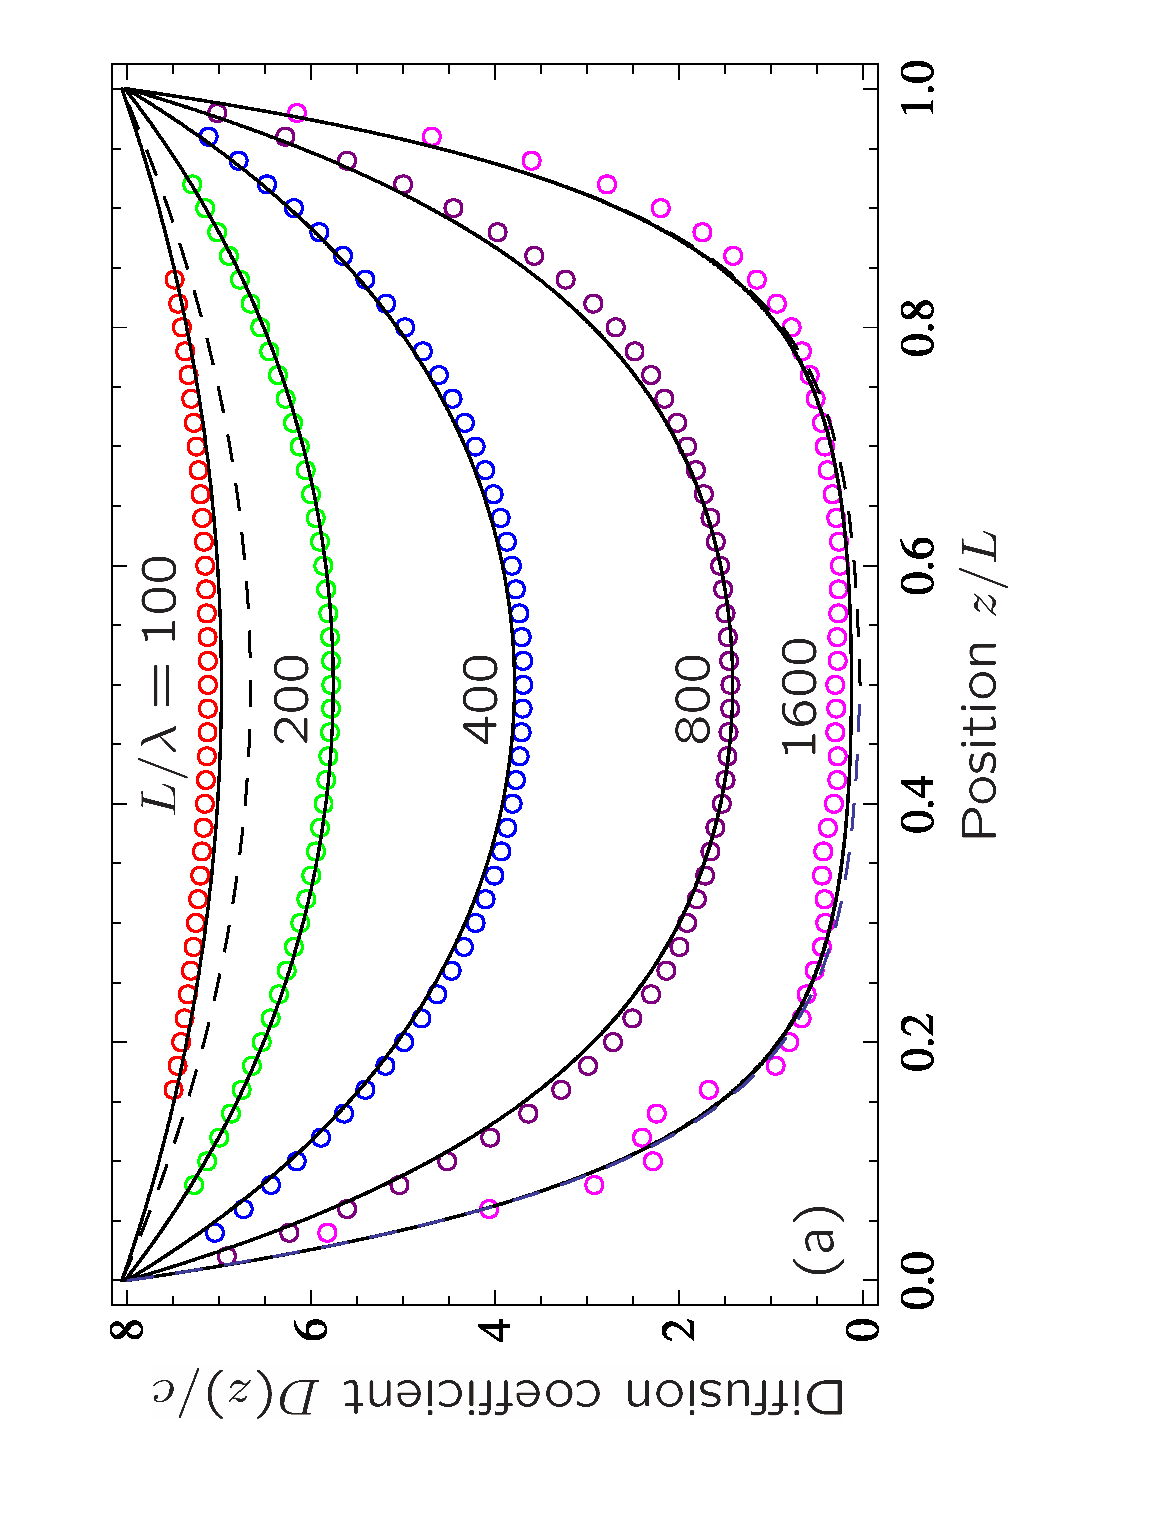
\includegraphics[height=5.5in,angle=-90]{fig2a}
%\vskip -1.25cm
%           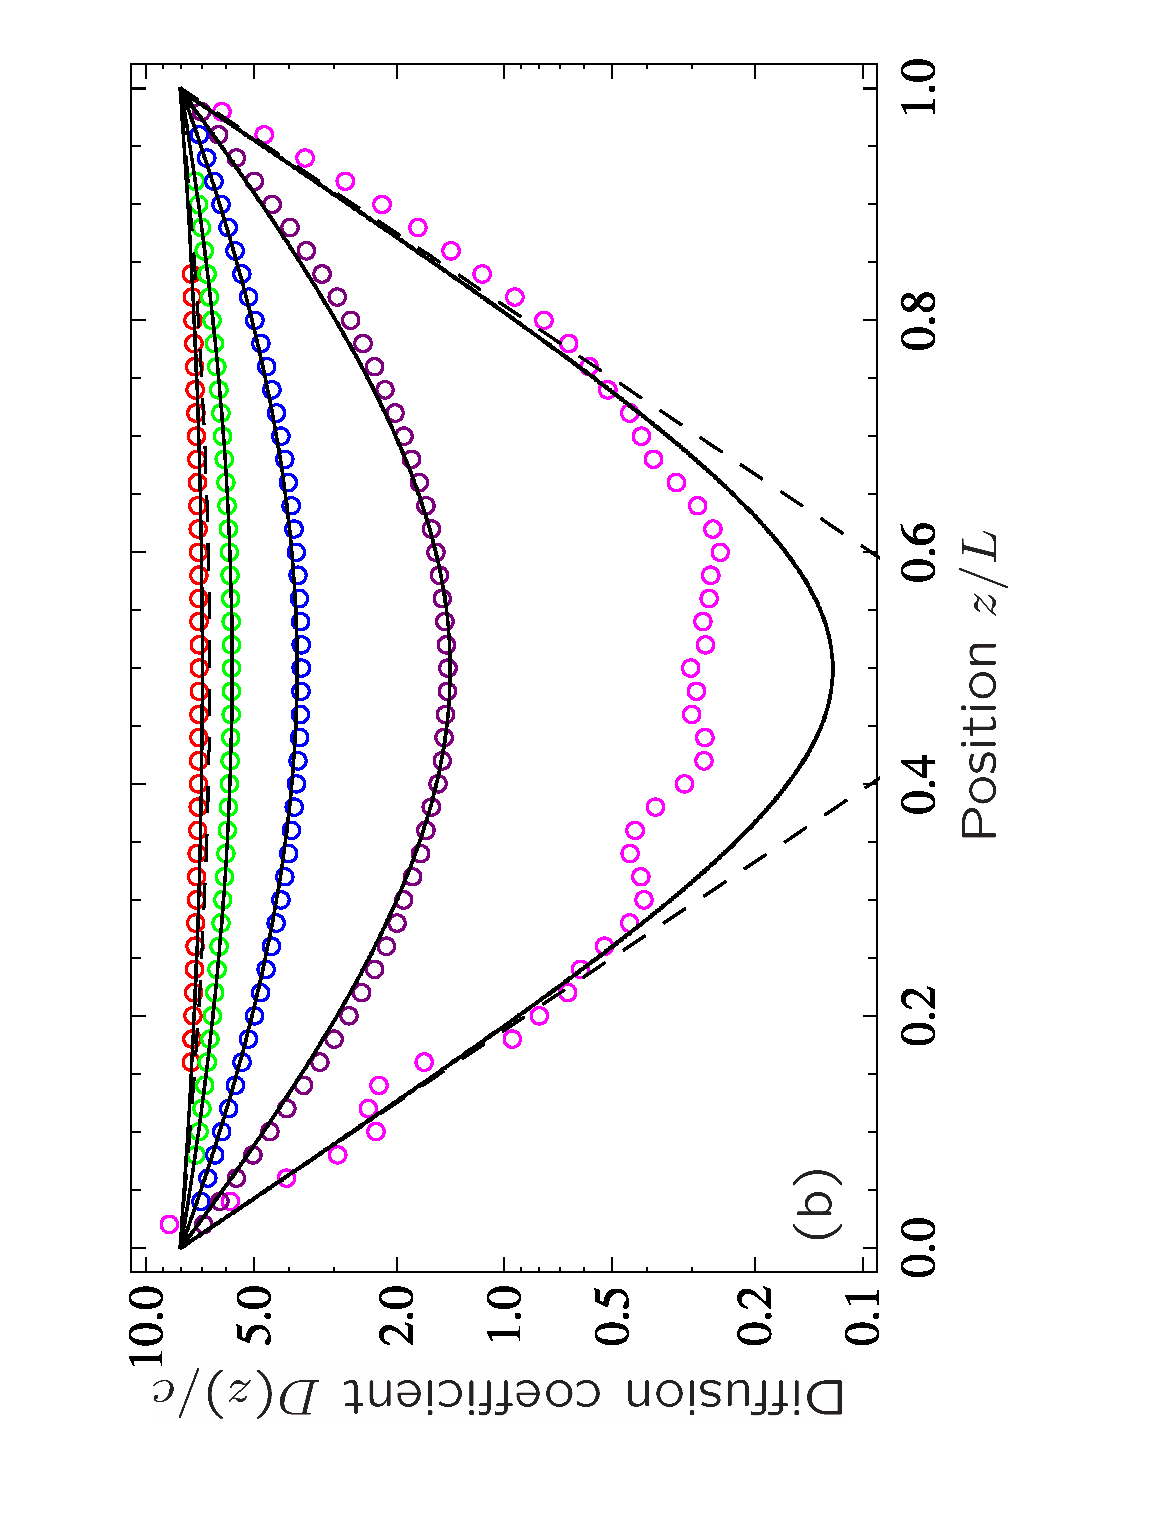
\includegraphics[height=5.5in,angle=-90]{fig2b}}
%\vskip -1cm
\vskip -0.5cm
\centering{\includegraphics[height=3.5in,angle=-90]{chapters/Anderson_Localization_as_position-dependent_diffusion_in_disordered_waveguides__Phys_Rev_B/pictures/fig2a}
\vskip -0.7cm
           \includegraphics[height=3.5in,angle=-90]{chapters/Anderson_Localization_as_position-dependent_diffusion_in_disordered_waveguides__Phys_Rev_B/pictures/fig2b}}
\vskip -0.7cm
\caption[(a) Position-dependent diffusion coefficient $D(z)$ in 2D waveguides supporting the same number $N = 10$ of transverse modes (width $w=5.25\lambda$) but having different lengths $L$.]{\label{fig2} (a) Position-dependent diffusion coefficient $D(z)$ in 2D waveguides supporting the same number $N = 10$ of transverse modes (width $w=5.25\lambda$) but having different lengths $L$. Disorder is the same for all lengths. Symbols show the results of numerical simulations, whereas solid lines are obtained from the self-consistent theory with the mean free path $\ell = 17.5\lambda$. Dashed lines show the approximate results for
$g_0 \gg 1$ (shown for $L = 100 \lambda$) and $g_0 \ll 1$ (shown for $L = 1600 \lambda$), with $D(0)$ substituted for $D_0$, see text. (b) Same as (a) but in the logarithmic scale.}
\end{figure}
%---------------------------------------------------------------------------------------------------------------------

The wave field $u(\mathbf{r})$ that we obtain as an outcome of the numerical algorithm allows us to calculate the energy density ${\cal W}(\mathbf{r})$ and flux $\mathbf{J}(\mathbf{r})$~\cite{1953_Morse}:
\begin{eqnarray}
{\cal W}({\bf r}) &=& \frac{k^2}{2}\left|u({\bf r})\right|^2 + \frac{1}{2}\left| \boldnabla u({\bf r})\right|^2, \label{eq:W}\\
{\bf  J}({\bf r}) &=& -kc\; \mathrm{Im} \left[u({\bf r})\boldnabla u({\bf r})\right]. \label{eq:J}
\end{eqnarray}
These two quantities formally define the diffusion coefficient $D(z)$ which, in general, may be position-dependent:
\begin{equation}
D(z) = -\frac{\langle J_z(\mathbf{r}) \rangle}{\frac{d}{d z} \langle{\cal W}(\mathbf{r}) \rangle},
\label{eq:Dofz_definition}
\end{equation}
where the averages $\langle \ldots \rangle$ are taken over a statistical ensemble of disorder realizations as well as over the crossection of the waveguide. Eq.~(\ref{eq:Dofz_definition}) can be used only at distances beyond one mean free path $\ell$ from the boundaries of the random medium because more subtle propagation effects of non-diffusive nature start to be important in the immediate vicinity of the boundaries~\cite{2007_Akkermans_book}.

We first consider non-absorbing disordered waveguides described by $\epsilon_a = 0$ in Eq.~(\ref{eq:helmholtz}) and real $\alpha$ in Eq.~(\ref{de}).
In Fig.~\ref{fig2} we compare numerical results for $D(z)$ with the outcome of SC theory for waveguides of different lengths but with statistically equivalent disorder. Quantitative agreement is observed for $L = 100$--$800 \lambda$, corresponding $g_0 \approx 0.3$--2. For the longest of our waveguides ($L = 1600\lambda$, $g_0 \approx 0.16$), deviations of numerical results from SC theory start to become visible in the middle of the waveguide, which is particularly apparent in the logarithmic plot of Fig.~\ref{fig2}(b).
The mean free path $\ell = 17.5\lambda$ corresponding to the best fit of SC theory to numerical results is only about $10\%$ higher than $\ell = 15.7 \lambda$ obtained from the fits in Fig.~\ref{fig1}.

We checked that the results of numerical simulations are not sensitive to the microscopic details of disorder: $D(z)$ obtained in two runs with different scattering strengths $\alpha$ and different scatterer densities, but equal mean free paths $\ell$ turned out to be the same.

%=====================================================================================================================
\section{EFFECT OF ABSORPTION}
\label{sec:absorption}

The linear absorption is modeled by introducing a non-zero $\epsilon_a$ in Eq.~(\ref{eq:helmholtz}) and making $\alpha$ in Eq.~(\ref{de}) complex. A link between $\epsilon_a$ and $\alpha$ can be established using the condition of flux continuity. Indeed, for continuous waves considered in this work the continuity of the flux leads to
\begin{equation}
\left\langle \boldnabla \cdot {\bf J}({\bf r})\right\rangle = (c/\ell_a) \left\langle{\cal W}({\bf r})\right\rangle,
\label{eq:flux_concervation}
\end{equation}
where $\ell_a = 1/k\epsilon_a$.
We checked that within numerical accuracy of our simulations the proportionality factor $c/\ell_a$ indeed remains constant independent of $z$. Therefore, Eq.~(\ref{eq:flux_concervation}) allows us to determine the microscopic absorption length $\ell_a$ as
$c \langle{\cal W}({\bf r})\rangle/\langle \boldnabla \cdot {\bf J}({\bf r})\rangle$ obtained numerically at a given $\alpha$.

%---------------------------------------------------------------------------------------------------------------------
\begin{figure}
%\vskip -1cm
%\centering{\includegraphics[height=5.5in,angle=-90]{fig3}}
%\vskip -1cm
\vskip -0.5cm
\centering{\includegraphics[height=3.5in,angle=-90]{chapters/Anderson_Localization_as_position-dependent_diffusion_in_disordered_waveguides__Phys_Rev_B/pictures/fig3}}
\vskip -0.7cm
\caption[The effect of absorption on the position-dependent diffusion coefficient.]{\label{fig3} The effect of absorption on the position-dependent diffusion coefficient. Symbols are results of numerical simulations in a 2D waveguide of length $L = 400\lambda$, width $w = 10.25 \lambda$ ($N = 20$) and several values of the macroscopic absorption length $L_a$ indicated on the figure. Lines are obtained from SC theory with $\ell = 17.1 \lambda$ adjusted to obtain the best fit for the case of no absorption (lower curve). Dashed line shows $D(z)$ following from the self-consistent theory with the same $\ell = 17.5 \lambda$ as in Fig.~\ref{fig2} and illustrates the sensitivity of $D(z)$ to the exact value of $\ell$.}
\end{figure}
%---------------------------------------------------------------------------------------------------------------------

Figure~\ref{fig3} demonstrates the effect of absorption on the position-dependent diffusion coefficient for a waveguide of length $L = 400\lambda$, which is about 25 mean free paths. For this waveguide $g_0 \simeq 1.3$ and the localization corrections are important. We observe that  absorption suppresses the localization correction to the position-dependent diffusion coefficient. This clearly demonstrates that the absorption nontrivially affects the transport by changing the way the waves interfere.
Nevertheless, we observe good agreement between numerical results (symbols) and SC theory (solid lines). The predictions of SC theory start to deviate from numerical results only for strong absorption ($L_a/L \lesssim 0.4$). Once again, the mean free path $\ell = 17.1 \lambda$ obtained from the fit of SC theory to the lower curve of Fig.~\ref{fig3} is within 10\% of the value estimated from the variance of dimensionless conductance.

%=====================================================================================================================
\section{CONCLUSIONS}
\label{sec:conclusions_Dz}

Two important results were obtained in this work. First, we convincingly demonstrated that the position-dependent diffusion coefficient is not an abstract mathematical concept but is a physical reality. The results of numerical simulations of scalar wave transport in disordered 2D waveguides unambiguously show that the onset of Anderson localization manifests itself as position-dependent diffusion. The reduction of the diffusion coefficient $D(\mathbf{r})$ is much more important in the middle of an open sample than close to its boundaries, in agreement with predictions of the self-consistent theory of localization.
Second, we established that for monochromatic waves in 2D disordered waveguides predictions of the self-consistent theory of localization are {\it quantitatively\/} correct provided that the dimensionless conductance in the absence of interference effects $g_0$ is at least larger than $0.5$. Moreover, the self-consistent theory yields a series expansion of the average conductance $\langle g \rangle$ in powers of $1/g_0$ that coincides exactly with the expansion obtained using the supersymmetry method~\cite{2000_Mirlin} up to terms of the order of $1/g_0^2$. This was not obvious {\it a priori\/} because of the numerous approximations involved in the derivation of self-consistent equations~\cite{2008_Cherroret}. The agreement between theory and numerical simulations is good in the presence of absorption as well, which has a particular importance in the context of the recent quest for Anderson localization of classical waves that heavily relies on confrontation of experimental results with the self-consistent theory~\cite{2004_Skipetrov,2008_van_Tiggelen_Nature,2006_Maret_PRL,2006_Skipetrov_dynamics,2003_Genack}. Deep in the localized regime ($g_0 < 0.5$), the self-consistent theory loses its quantitative accuracy, but still yields qualitatively correct results (exponential decay of conductance with the length of the waveguide and of the diffusion coefficient $D$ with the distance from waveguide boundaries). It would be extremely interesting to see if the ability of the self-consistent theory to provide quantitative predictions still holds in three-dimensional systems where a mobility edge exists. In particular, the immediate proximity of the mobility edge is of special interest.

\textit{Note added.}
After this paper was submitted for publication, a related preprint appeared~\cite{2010_Tian_PRL}. In particular, the authors of that work show that the self-consistent theory does not apply to 1D disordered media, which is consistent with our results because $g_0 \sim \ell/L$ is always small in 1D, provided that the condition $L \gg \ell$ assumed in this paper is fulfilled.

%=====================================================================================================================
%\acknowledgments
%\ \\
%\textbf{Acknowledgments}
\section{ACKNOWLEDGMENTS}

We thank Bart van Tiggelen for useful comments. The work at Missouri S\&T was supported by the National Science Foundation Grant No. DMR-0704981. The numerical results obtained at the Tera-Grid, award Nos. DMR-090132 and DMR-100030. S.E.S. acknowledges financial support of the French ANR (Project No. 06-BLAN-0096 CAROL).

\label{paper:4_end}

\PaperManuscript{5}{Mapping algorithm from the two-dimensional aperiodic Thue-Morse structure to the square lattice}
% to be submitted
% /svn/research/Project_DAS/2012_Mapping_2D_TM_manuscript
\setcounter{section}{0}
\setcounter{figure}{0}
\setcounter{table}{0}
\label{paper:5_start}
% \documentclass[final,5p,times,twocolumn]{elsarticle}
% %\documentclass[preprint,review,12pt]{elsarticle}
% \usepackage{hyperref} %% optional
% \usepackage{amssymb}
% \usepackage{amsmath}
% \biboptions{compress}
% 
% \newcounter{bla}
% \newenvironment{refnummer}{%
% \list{[\arabic{bla}]}%
% {\usecounter{bla}%
%  \setlength{\itemindent}{0pt}%
%  \setlength{\topsep}{0pt}%
%  \setlength{\itemsep}{0pt}%
%  \setlength{\labelsep}{2pt}%
%  \setlength{\listparindent}{0pt}%
%  \settowidth{\labelwidth}{[9]}%
%  \setlength{\leftmargin}{\labelwidth}%
%  \addtolength{\leftmargin}{\labelsep}%
%  \setlength{\rightmargin}{0pt}}}
%  {\endlist}
% 
% 
% \journal{Computer Physics Communications}
% 
% \begin{document}
% 
% \begin{frontmatter}
% 
\chapter{Mapping algorithm from the two-dimensional aperiodic Thue-Morse structure to the square lattice}
\label{chap:TM_to_TB}
\label{paper:5_start}

\begin{center}
Ben Payne$^1$, Heeso Noh$^2$, Hui Cao$^2$, and Alexey Yamilov$^1$                                                                               \end{center}

\ \\
% \author[a]{Ben Payne\corref{author}}
% \author[b]{Heeso Noh}
% \author[b]{Hui Cao}
% \author[a]{Alexey Yamilov}
\begin{center}
\textit{$^1$Department of Physics, Missouri University of Science \& Technology,\\ Rolla, MO 65409\\
$^2$Department of Applied Physics, Yale University, New Haven, CT 06520}\end{center}

\ \\
% 
% \cortext[author] {Corresponding author.\\\textit{E-mail address:} benjamin.payne@mst.edu}
% \address[a]{Department of Physics, Missouri University of Science \& Technology, Rolla, Missouri 65409, USA}
% \address[b]{Department of Applied Physics, Yale University, New Haven, Connecticut 06520-8482, USA}
% 
% \begin{abstract}
\addcontentsline{toc}{section}{ABSTRACT}
\begin{center}\textbf{ABSTRACT\footnote{In preparation for Journal of Physics A (2012).}}        \end{center}

Deterministic aperiodic structures, such as those obtained via the Thue-Morse algorithm, exhibit a variety of unusual transport properties not found in either ordered or random media. The non-periodic nature of this system makes it notoriously difficult to characterize theoretically, especially in dimensions higher than one. Here, we demonstrate the possibility of mapping the two-dimensional aperiodic Thue-Morse pattern of micro-cavities onto a square lattice, making it easily amenable to the tight-binding description. We also show that only three distinct nearest and three next-nearest micro-cavity arrangements exist. An implementation of this mapping procedure in Matlab is provided. 
% \end{abstract}
% 
% \begin{keyword}
% Aperiodic structure \sep Thue-Morse sequence
% \end{keyword}
% 
% \end{frontmatter}

% {\bf PROGRAM SUMMARY}
% 
% \begin{small}
% \noindent
% {\em Manuscript Title:} Mapping algorithm from the two-dimensional aperiodic Thue-Morse structure to the square lattice \\
% {\em Authors:} Ben Payne, Heeso Noh, Hui Cao, Alexey Yamilov                      \\
% {\em Program Title:} thuemorse\_to\_square\_mapping\\
% {\em Journal Reference:}                                      \\
% {\em Catalogue identifier:}                                   \\
% {\em Licensing provisions:} Common                         \\
% {\em Programming language:}  Matlab \\ % tested with Matlab 7.10.0.499 (R2010a)
% {\em Computer:} personal computer running Matlab      \\
% {\em Operating system:} Operating system sufficient to run Matlab   \\
% {\em RAM:} 1 Gigabyte                                              \\
% {\em Keywords:} Aperiodic structure, Thue-Morse sequence  \\
% {\em Classification:} 7.9 Transport Properties, 18 Optics            \\
% {\em Nature of problem:} The Thue-Morse algorithm generates a two-dimensional (2D) binary array which is not translationally invariant. This pattern can be used to fabricate an aperiodic 2D array of optical micro-cavities. We show this array can be reduced to a square (periodic) lattice, making possible the application of powerful theoretical analysis based on the tight-binding description.  \\
% {\em Solution method:} By identifying underlying structure in the 2D Thue-Morse sequence, we demonstrate the possibility of mapping onto the 2D square lattice with a finite set of local coupling arrangements. \\
% {\em Restrictions:} The maximum size of the resulting array is limited by computer memory. Input parameter generation $g$ with values from 5 to 12 have been tested, which result in arrays of size $2^5$ to $2^{12}$, respectively. \\
% {\em Unusual features:} None.\\
% {\em Additional comments:} None.\\
% {\em Running time:} Less than 3 minutes on current desktop computers (Intel Pentium 4 3.2Ghz CPU, 4GB RAM). \\
% \end{small}


\section{INTRODUCTION}
\label{sec:introduction_mapping}

Deterministic aperiodic structures (DAS)~\cite{2009_Barber} lie between periodic and random, ranging from quasi-crystals to pseudo-random arrangements. Unlike crystals, they do not have translational symmetry. In contrast with random media, DAS are defined by mathematical rules and have long-range order. {\it Photonic} deterministic aperiodic nano-structures can now be routinely prepared with a variety of nano-fabrication techniques~\cite{2011_Dal_Negro_DAS_review}.

An exhaustive classification of quasi-periodic and aperiodic systems can be accomplished based on an analysis of the structure factor~\cite{2010_Ivchenko}. Quasiperiodic (e.g.~Fibonacci sequence) arrangements are characterized by a pure point spectrum. Exhibiting higher levels of complexity, aperiodic structures can be further subdivided into those having either a singular continuous spectrum or an absolutely continuous spectrum~\cite{2006_Macia}. The prominent example in the former class is the Thue-Morse~\cite{1921_Morse} sequence -- the focus of this study. 
 
Previous studies of Thue-Morse structures revealed highly anomalous transport properties and unusual energy spectra with self-similar features~\cite{1988_Cheng_Thue_Morse,1989_Luck}. One-dimensional (1D) photonic Thue-Morse structures~\cite{1997_Liu,2004_Negro,2004_Qiu,2005_Agarwal,2005_Joannopoulos,2007_Agarwal} are amenable to a variety of theoretical treatments~\cite{2009_Barber,2010_Ivchenko}. Higher dimensional structures are predicted to display richer behaviors~\cite{2011_Dal_Negro_DAS_review}, just as wave transport in two-dimensional~(2D) random media is more complicated than in~1D~\cite{1979_Anderson}. This observation is indeed supported by the theoretical~\cite{2007_Moretti,2008_Boriskina} and  experimental studies on 2D Thue-Morse DAS that recently appeared in literature~\cite{2004_Negro,2007_Agarwal,2009_Boriskina,2007_Matsui,2008_Gopinath_DAS,2011_Cao_DAS}. Despite the practical interest in the 2D systems, the increased complexity (compared to the 1D counterparts) limits the availability of analytical approaches. The tight binding approximation is generally unavailable in photonic systems, contributing to the problem.

Two-dimensional Thue-Morse DAS can be created by selectively removing particles from a 2D square lattice~\cite{2011_Dal_Negro_DAS_review,2008_Gopinath_DAS}. This process generates a pattern of~$2\times2$ micro-cavities, c.f.~Fig.~\ref{fig:mapping_procedure}, which exhibits self-similar structure on progressively larger scales. These micro-cavities can support confined modes~\cite{2007_Moretti,2008_Boriskina}, similar to whispering gallery modes of micro-disk resonators. Patterns of coupling between the cavity modes in the Thue-Morse structure plays an important role in determining the lasing mode profile~\cite{2011_Cao_DAS}. 

The goal of this work is to demonstrate the possibility of mapping the micro-cavity array in the 2D aperiodic Thue-Morse structure onto a square lattice. We provide a Matlab numerical code which identifies {\it exactly four nearest and four next-nearest neighbors of each cavity}. It is demonstrated that only three types of neighboring arrangements exist in the Thue-Morse structure, allowing assignment of nearest and next-nearest neighbor coupling coefficients to each micro-cavity. Thus, we accomplish the reduction of 2D {\it aperiodic} Thue-Morse array to the {\it periodic} square array of micro-cavities with {\it aperiodic couplings}. Our finding opens up the possibility of a thorough theoretical investigation based on the tight binding Hamiltonian description~\cite{2009_Barber}.

\begin{figure}%[h]
\begin{flushleft} 
%\begin{Large}
\ \ \ (a)
%\end{Large}
\end{flushleft}
\vskip -0.3in
\centering{\includegraphics[width=2.4in,angle=0]{chapters/Mapping_algorithm_from_the_two-dimensional_aperiodic_Thue-Morse_structure_to_the_square_lattice/pictures/fig1a_TM_2D_gen6_scatterers_dots}}
\begin{flushleft} 
%\begin{Large}
\ \ \ (b)
%\end{Large}
\end{flushleft}
\vskip -0.2in
\centering{\includegraphics[height=2.4in,angle=0]{chapters/Mapping_algorithm_from_the_two-dimensional_aperiodic_Thue-Morse_structure_to_the_square_lattice/pictures/fig1b_TM_2D_gen6_scatterers_with_squares}}
\begin{flushleft} 
%\begin{Large}
\ \ \ (c)
%\end{Large}
\end{flushleft}
\vskip -0.2in
\centering{\includegraphics[width=1.5in,angle=0]{chapters/Mapping_algorithm_from_the_two-dimensional_aperiodic_Thue-Morse_structure_to_the_square_lattice/pictures/fig1c_TM_2D_gen6_scatterers_collapsed}}
\caption[(a)~The 2D Thue-Morse structure of generation $g=6$~($64\times64$ elements).]{\label{fig:mapping_procedure} (a)~The 2D Thue-Morse structure of generation $g=6$~($64\times64$ elements). After populating the 2D square lattice with binary elements~$A$ and~$B$ via the inflation procedure $A\rightarrow AB$ and $B\rightarrow BA$; $A$~is interpreted as the positions of scatters. (b)~Same as~(a) with the $2\times2$ clusters regions void of scatters highlighted. These regions play the role of optical micro-cavities in the experiment~\cite{2011_Cao_DAS}. (c) The array of micro-cavities in (b) after the collapse procedure of removing rows and columns void of cavities, see text. The collapsed structure is a periodic square lattice rotated by $45^\circ$; it facilitates identification of the neighboring cavities.}
\end{figure}

\section{MAPPING MICRO-CAVITIES IN 2D THUE-MORSE ARRAY \\ONTO SQUARE LATTICE}

Construction of the 2D Thue-Morse pattern is accomplished in two steps \cite{2008_Negro}. {\it Step~1:} The 1D Thue-Morse sequence is generated by starting with letter~$A$ (generation $g=0$) and repeatedly applying the inflations rules $A\rightarrow AB$ and $B\rightarrow BA$. After repeating the procedure $g$ times the number of elements in the binary sequence is~$2^g$. The complimentary system is defined as $A\rightarrow B$ and $B\rightarrow A$. {\it Step~2:} Using the~$2^g$ elements of the 1D sequence obtained in Step~1 as seeds, we build 1D Thue-Morse sequences of $g$'th generation along the second dimension of the structure. $A$~elements in the resulting~$2^g\times2^g$ array define the position of the ``particles,'' e.g.~cylindrical holes in a dielectric membrane~\cite{2011_Cao_DAS}.  
%\href{http://mathworld.wolfram.com/Thue-MorseSequence.html}{Mathworld figure}

Figure~\ref{fig:mapping_procedure}(a) shows the 2D Thue-Morse structure with $g=6$ obtained using the above procedure. We observe the occurrence of micro-cavities formed at the places missing $2\times2$ holes. Holes surrounding a cavity in the dielectric membrane~\cite{2011_Cao_DAS} create a mismatch in the effective refractive index between the inside and outside regions. Hence, the micro-cavity regions can support cavity modes and play an important role in determining transport properties of the system~\cite{2007_Moretti,2008_Boriskina}. 

Figure~\ref{fig:mapping_procedure}(b) highlights the cavity regions in the 2D Thue-Morse structure. The cavities occur only in the columns with identical adjacent seeds, c.f. Step~1 in the construction procedure above. Indeed, by construction, the columns generated from a pair of dissimilar seeds (i.e. $\ldots AB \ldots$ or $\ldots BA \ldots$) can never contain $2\times2$ clusters. The same argument can also be made regarding the rows in the pattern depicted in Fig.~\ref{fig:mapping_procedure}. Hence, the following {\it collapse procedure} can be performed: one drops all columns and all rows void of the $2\times2$ clusters. The result of this operation is a perfectly periodic square lattice of cavities rotated by $45^\circ$, c.f. Fig.~\ref{fig:mapping_procedure}(c). In this state one can {\it uniquely} identify exactly four nearest and four next-nearest neighbors of each cavity. In the next section, we revert to the original structure {\it expansion procedure} to study the patterns in arrangements of the neighbors.

\section{EXHAUSTIVE ENUMERATION OF INTER-CAVITY ARRANGEMENTS}

\begin{figure}%[h]
% \begin{flushleft}
% \begin{Large}
% (a)\hskip 1.5in (b)
% \end{Large}
% \end{flushleft}
%\vskip -0.3in
\centering{
(a) \hskip 0.2in
\includegraphics[scale=0.13,angle=0]{chapters/Mapping_algorithm_from_the_two-dimensional_aperiodic_Thue-Morse_structure_to_the_square_lattice/pictures/fig2a_TM_2D_scatterers_purple_nearest_neighbor_couplings}
%\hskip 0.3in
 \hskip 0.2in (b)  \hskip 0.2in
\includegraphics[scale=0.13,angle=0]{chapters/Mapping_algorithm_from_the_two-dimensional_aperiodic_Thue-Morse_structure_to_the_square_lattice/pictures/fig2b_TM_2D_scatterers_purple_next-nearest_neighbor_couplings}}
\caption[(a) Nearest neighbor and (b) next-nearest neighbor arrangements of micro-cavities in 2D Thue-Morse pattern.]{\label{fig:nn_and_nnn_couplings} (a) Nearest neighbor and (b) next-nearest neighbor arrangements of micro-cavities in 2D Thue-Morse pattern. The identification of a neighboring cavity is based on Fig.~\ref{fig:mapping_procedure}c and the coupling type is determined from Fig.~\ref{fig:mapping_procedure}b.}
\end{figure}

After identifying neighboring cavities in the previous section,~c.f. Fig.~1(c), we now turn to the analysis of coupling. The collapse procedure introduced above demonstrates that the furthest separation between next nearest neighbors is equal to six (in the units of lattice constant of the original structure). This observation, and the fact that the Thue-Morse structure by construction contains a finite number of distinct blocks of a given size, leads to the conclusion that the number of distinct cavity couplings should also be finite. Indeed, we find that there are only three distinct nearest and three distinct next-nearest neighbor configurations, c.f.~Fig.~\ref{fig:nn_and_nnn_couplings}~and~\ref{fig:couplings_Hamiltonian}. All cavity configurations can be obtained from these sets by rotation or mirror symmetry transformations. 

The physical significance of a finite number of cavity neighbor arrangements in the Thue-Morse structure is that it results in a finite number of inter-cavity couplings in the tight binding description of the system. The tight-binding model~\cite{1954_Slater_tightBinding} has been a powerful tool in studies of DAS~\cite{2009_Barber}. The Thue-Morse pattern has been treated with the tight-binding model in 1D, where neighbors are clearly defined~\cite{1995_Carpena}. Applying the tight-binding model in 2D is expected to be a fruitful approach in describing transport in the Thue-Morse system~\cite{2011_Cao_DAS}. At the eigenfrequency of the cavity mode, transport is dominated by the coupling between microcavities. Thus, we write
\begin{equation}
E_0\ \psi_{ij}+\sum_{i^\prime j^\prime}c_{ij,i^\prime j^\prime}\ \psi_{i^\prime j^\prime}=E\ \psi_{ij},
\label{eq:2D_array_sites}
\end{equation}
where $E_0$ is the energy of an isolated cavity and $\psi_{ij}$ is the field amplitude of the $ij$'th cavity. Indices $i$ and $j$ enumerate the cavities based on the collapse procedure shown in Fig.~\ref{fig:mapping_procedure}(c). Further, $c_{ij,i^\prime j^\prime}$ denote the couplings between the cavities located at $ij$ and $i^\prime j^\prime$. The analysis of physical proximity in the Thue-Morse structure, c.f.~Fig.~\ref{fig:mapping_procedure}(b), allows us to limit the consideration to two types of coupling -- nearest ($i^\prime=i\pm1$ and $j^\prime=j$, or $i^\prime=i$ and $j^\prime=j\pm1$) and next-nearest ($i^\prime=i\pm1$ and $j^\prime=j\pm1$) couplings only. From Fig.~\ref{fig:nn_and_nnn_couplings} it follows that $c_{ij,i^\prime j^\prime}$ can take one of only six possible values, three of each type. This constitutes the main result of this work. As an example, we used the numerical code described in the next section to generate the color-coded pattern of nearest and next-nearest couplings (four of each type) for the 2D Thue-Morse structure of generation~$g=6$, c.f.~Fig.~\ref{fig:couplings_Hamiltonian}. Thus, the structural complexity in the arrangement of cavities in the original pattern has been reduced to the complexity in connectivities between the elements of the ordered array in Eq.~(\ref{eq:2D_array_sites}).

\begin{figure}%[h]
\begin{flushleft}
%\begin{Large}
(a)
%\end{Large}
\end{flushleft}
\vskip -0.1in
\centering{\includegraphics[width=3.5in]{chapters/Mapping_algorithm_from_the_two-dimensional_aperiodic_Thue-Morse_structure_to_the_square_lattice/pictures/fig3a_nn_color_coded_no_labels_bw_no_colorbar}}
\begin{flushleft}
%\begin{Large}
(b)
%\end{Large}
\end{flushleft}
\vskip -0.1in
\centering{\includegraphics[width=3.5in]{chapters/Mapping_algorithm_from_the_two-dimensional_aperiodic_Thue-Morse_structure_to_the_square_lattice/pictures/fig3b_nnn_color_coded_no_labels_bw_no_colorbar}}
\caption[Four corners of each cavity represent four nearest (a) or four next-nearest (b) couplings of the $2\times 2$ micro-cavities in the 2D Thue-Morse array of generation $g=6$.]{\label{fig:couplings_Hamiltonian} Four corners of each cavity represent four nearest (a) or four next-nearest (b) couplings of the $2\times 2$ micro-cavities in the 2D Thue-Morse array of generation~$g=6$. The results are obtained using the provided Matlab code.}
\end{figure}

\section{DESCRIPTION OF MATLAB CODE}

The supplied code is an implementation of the described algorithm in the Matlab scripting language. Inputs to the primary function are the generation~$g$, complementarity, and a boolean for creating plots. The generation of the Thue-Morse pattern must be a positive integer; values of~$g$ up to 12 have been verified. However, when~$g$ is less than~5 the pattern is too small to show nearest neighbor coupling. The second input, complementarity, allows one to generate the standard Thue-Morse pattern or its complimentary obtained by simultaneous replacement $A\rightarrow B$ and $B\rightarrow A$ throughout the pattern~-- values 0~or~1 respectively. The last input parameter is a boolean switch defining whether or not to generate graphical representations of the results and takes values 0~or~1. After input values are specified by the user, the 2D Thue-Morse pattern is created. The initial size is a square with sides of length~$2^g$. 

For each site in the 2D array, the surrounding pattern is used to determine whether the site is part of a micro-cavity, or if it is part of the buffer in one of three nearest neighbor coupling arrangements. The specific local pattern of the neighboring sites for any given site has only four possible outcomes, the result of which is stored to a three dimensional array of size $2^g\times2^g\times6$. The first layer has four possible values to denote whether a site is part of a micro-cavity or one of the three nearest-neighbor coupling types. The second of the six layers describes whether a site within a $2\times 2$ microcavity is locally in the top, left, right, or bottom position. In the third layer, the nearest neighbor coupling type is recorded for each micro-cavity, c.f.~Fig.~\ref{fig:nn_and_nnn_couplings}a, and the next-nearest coupling type is in the fourth layer of the storage array. Lastly, the original~$x$ and~$y$ coordinates of each site are in the fifth and sixth layers, respectively. 

To determine next-nearest neighbor coupling, micro-cavities sufficiently far from the edges of the 2D array are found. Then, for each micro-cavity, the four next-nearest neighbors are located based on the site arrangement, c.f.~Fig.~\ref{fig:nn_and_nnn_couplings}b, similar to the nearest neighbor procedure above. This result is recorded in layer four of the storage array.

At this stage, all relevant information has been determined. Next, only rows and columns containing micro-cavities are retained, whereas the edges of the 2D Thue-Morse system containing neither nearest nor next-nearest neighbors are discarded. Two arrays, each of size $2^g\times 2^g$, are returned by the main function. These arrays specify nearest and next-nearest coupling types, respectively. 

\section{CONCLUSION}

In this work, we demonstrated the possibility of mapping the array of micro-cavities in the 2D Thue Morse deterministic aperiodic system onto a periodic square lattice. Such mapping allowed us to uniquely identify and exhaustively enumerate the configurations of nearest and next-nearest neighbors. We found that only three configurations of each type exist. Thus, we accomplished the reduction of the original aperiodic structure to the periodic structure with aperiodic arrangement of the limited set of pairings. We developed and provided with this paper a Matlab simulation code which performs this cavity identification and mapping procedure. The results will be used for future investigations of novel transport properties expected in 2D DAS structures. 

\section{ACKNOWLEDGEMENTS}

Authors acknowledge support by National Science Foundation under Grants No. DMR-0704981 and No. DMR-0808937.
% 
% \bibliographystyle{elsarticle-num}
% \bibliography{../../Bibliography/latex_bibliography}
% 
% \end{document}


 
\label{paper:5_end}

\PaperManuscript{6}{2D Thue-Morse array of optical cavities: tight-binding model}
% to be submitted
% /svn/research/Project_DAS/2012_TB_for_2DTM_manuscript
\setcounter{section}{0}
\setcounter{figure}{0}
\setcounter{table}{0}
\label{paper:6_start}
% \documentclass[prb,showpacs,amsmath,amssymb,twocolumn]{revtex4}
% 
% \usepackage{dcolumn}
% \usepackage{verbatim}
% \usepackage{graphicx}
% \usepackage{epsfig} % multi-line comments
% \usepackage{hyperref}
% 
% \begin{document}
% \newcommand{\boldnabla}{\mbox{\boldmath$\nabla$}}
% 
\chapter{2D THUE-MORSE ARRAY OF OPTICAL CAVITIES: TIGHT-BINDING MODEL}
\label{eq:TM_physics}
\label{paper:6_start}

% 
\begin{center}
Ben Payne$^1$, Laura Sisken$^1$, Heeso Noh$^2$, Hui Cao$^2$, Alexey Yamilov$^1$                                                                               \end{center}

\ \\
% \author{Ben Payne$^1$, Laura Sisken$^1$, Heeso Noh$^2$, Hui Cao$^2$, Alexey Yamilov$^1$ \footnote{Electronic~address:~yamilov@mst.edu}}
\begin{center}
\textit{$^1$Department of Physics, Missouri University of Science \& Technology,\\ Rolla, MO 65409\\
$^2$Department of Applied Physics, Yale University, New Haven, CT 06520}\end{center}

\ \\
% \affiliation{$^1$Department of Physics, Missouri University of Science \& Technology, Rolla, MO 65409\\
% $^2$Department of Applied Physics, Yale University, New Haven, CT 06520}
% 
% \date{\today}
% 
% \begin{abstract}
\addcontentsline{toc}{section}{ABSTRACT}
\begin{center}\textbf{ABSTRACT\footnote{In preparation for Physical Review B (2012).}}\end{center}

We report on a study of optical properties of a two-dimensional array of micro-cavities spatially arranged according to the Thue-Morse sequence. The Thue-Morse structure is a prime example of deterministic aperiodic systems with singular-continuous spatial Fourier spectra. In a realistic system we establish applicability of the tight-binding description. This description is employed to investigate coexisting localized and delocalized states and their scaling dependence on the size of the structure.
% \end{abstract}
% 
% % 42.25.Dd - Wave propagation in random media
% % 72.15.Rn - Localization effects (Anderson or weak localization) 
% \pacs{42.25.Dd,72.15.Rn}
% 
% \maketitle

% Notation: ``Pairing'' is a geometrical concept relevant to a pattern. ``Coupling'' is a physics concept associated with the tight-binding approach.

\section{INTRODUCTION}
\label{sec:introduction_TB}

Non-periodic structures occupy the place between periodic and random structures, ranging from quasi-crystals to pseudo-random structures~\cite{2006_Macia}. These deterministic aperiodic structures (DAS) are obtained iteratively according to some predetermined rules, and have long-range order~\cite{2009_Barber}. The structural complexity of DAS is measured by their spatial Fourier spectra or structure factor. The three major classes of DAS, with increasing degree of complexity, have singular, singular-continuous, and absolutely continuous spectra~\cite{2006_Macia}. Hence, DAS span the entire hierarchy of complexity. Because of their structural distinction and unusual physical properties, the aperiodic systems have been called the third form of solid matter~\cite{2010_Ivchenko}. {\it Photonic} deterministic aperiodic nano-structures can now be routinely prepared with a variety of nano-fabrication techniques~\cite{2011_Dal_Negro_DAS_review}.

The Thue-Morse sequence~\cite{1921_Morse} has a singular-continuous spatial Fourier spectrum, combining the properties of both periodic and random media. Previous studies of Thue-Morse structures revealed highly anomalous transport properties, such as co-existence of extended and localized states~\cite{1992_Ryu} as well as the appearance of spectral windows of complete optical transparency~\cite{2004_Peng}. Related to the above is an unusual self-similar energy spectrum~\cite{1988_Cheng_Thue_Morse,1989_Luck}. 

One-dimensional~(1D) photonic Thue-Morse structures~\cite{1997_Liu,2004_Negro,2004_Qiu,2005_Agarwal,2005_Joannopoulos,2007_Agarwal} are readily amenable to a variety of theoretical treatments~\cite{2009_Barber,2010_Ivchenko}. Higher dimensional structures are predicted to display richer behaviors~\cite{2011_Dal_Negro_DAS_review}, just as wave transport in two-dimensional~(2D) random media is more complicated than in~1D~\cite{1979_Anderson}. This observation is indeed supported by both the theoretical~\cite{2007_Moretti,2008_Boriskina} and the experimental studies on 2D Thue-Morse DAS that recently appeared in literature~\cite{2004_Negro,2007_Agarwal,2008_Negro,2009_Boriskina,2007_Matsui,2008_Gopinath_DAS,2011_Cao_DAS}. 

Despite practical interest in the 2D systems, the increased complexity (compared to their 1D counterparts) limits the availability of analytical approaches. Adapting the methods for 1D systems, e.g., trace map analysis~\cite{1997_Liu, 1987_kohmoto,2007_Lei,1995_Chakrabarti,1989_Luck,2000_Wang}, time evolution method~\cite{1997_Lahiri}, perturbation approach~\cite{1995_Peng}, renormalization group method~\cite{1986_Niu,1983_Southern,1998_Ghosh}, and numerical transfer matrix analysis~\cite{1997_Pelster,2004_Peng, 2000_Peng,2003_Qiu,2004_Qiu,2007_Hiltunen}, to higher dimensional systems is not straightforward.

The goal of this work is to demonstrate the possibility of studying light transport in 2D photonic Thue-Morse DAS with the tight-binding model. The tight-binding model, which yielded such enormously important theoretical results as demonstration of Anderson localization~\cite{1958_Anderson,2009_Lagendijk_PT}, has been a powerful tool in studies of electronic properties of quasi-crystals~\cite{2003_Trebin_Quasicrystals}. Because photons, unlike electrons, cannot be easily confined by single scattering centers, a tight-binding description is not usually applicable. This limitation can be overcome by creating optical cavities with structural defects inside a photonic crystal. Photons may be confined in individual cavities and tunnel to adjacent cavities. 

2D Thue-Morse DAS are created by selectively removing particles from a 2D square lattice~\cite{2011_Dal_Negro_DAS_review,2008_Gopinath_DAS}. The process generates a pattern of~$2\times2$ micro-cavities, c.f.~Fig.~\ref{fig:ThMo_reduction}(a), that exhibits self-similar structure on progressively larger scales. These micro-cavities can support confined modes~\cite{2007_Moretti,2008_Boriskina}. Patterns of coupling between the cavity modes in the Thue-Morse structure plays an important role in determining the lasing mode profile~\cite{2011_Cao_DAS}. Previously we have shown that the complexity in the spatial arrangement of the micro-cavities can be replaced by the complexity of correlated couplings in a (periodic) square lattice of micro-cavities~\cite{2012_Payne_Mapping_2D_TM}. We employ this mapping procedure to obtain and diagonalize the tight-binding Hamiltonian allowing us to make predictions regarding the nature of the eigenmodes and their finite size scaling properties.

In this work we demonstrate that under realistic experimental conditions, the tight-binding treatment can be applicable to a 2D Thue-Morse based array of micro-cavities. In Section~\ref{sec:design} we describe construction of a 2D Thue-Morse based array of micro-cavities and demonstrate the applicability of the tight-binding description under realistic conditions in Ref.~\citenum{2011_Cao_DAS}. In Sec.~\ref{sec:tb} we investigate both the size scaling of the density of states and the inverse participation ratio within the framework of the tight-binding model. We conclude with a discussion of implications of our results in Sec.~\ref{sec:conclusions_TB}.

\section{STRUCTURE DESIGN AND OPTIMIZATION}
\label{sec:design}

\begin{figure}
\centering{\includegraphics[width=1.6in]{chapters/2D_Thue-Morse_array_of_optical_cavities_tight-binding_model/pictures/fig1a_experimental_sem_top_view}
           \includegraphics[width=1.75in]{chapters/2D_Thue-Morse_array_of_optical_cavities_tight-binding_model/pictures/fig1b_experimental_sem_side_view}}
\caption[Top-view SEM image of a 2D Thue-Morse array of air holes in the GaAs membrane.]{\label{fig:experimental_structure}
Left: top-view SEM image of a 2D Thue-Morse array of air holes in the GaAs membrane. Right: tilt-view SEM image of a cleaved sample showing the perforated GaAs membrane free standing in air. White scale bars from left to right are 2$\mu$m and 500nm.}
\end{figure}

The 2D Thue-Morse pattern is usually constructed in two steps~\cite{2008_Negro}. First, the 1D Thue-Morse sequence is generated by starting with letter~$A$ (generation $g=0$) and repeatedly applying the inflation rules $A\rightarrow AB$ and $B\rightarrow BA$. After $g$ iterations the number of elements in the binary sequence is~$2^g$. The complimentary system is obtained by simultaneous replacements of $A\rightarrow B$ and $B\rightarrow A$. In the second step, using the~$2^g$ elements of the 1D sequence obtained previously as seeds, we build 1D Thue-Morse sequences of $g$'th generation along the second dimension of the structure. $A$~elements in the resulting~$2^g\times2^g$ array define the position of the ``particles,'' such as e.g. cylindrical holes in a dielectric membrane, c.f. Fig.~\ref{fig:experimental_structure}. 

Figure~\ref{fig:ThMo_reduction}(a) depicts the 2D Thue-Morse structure with $g=6$ obtained using the above procedure. We observe the occurrence of clusters formed at the places of missing $2\times2$ holes. Holes surrounding a cavity in the dielectric membrane~\cite{2011_Cao_DAS} create a mismatch in the effective refractive index between the inside and outside regions. Hence, in certain spectral ranges the cluster regions can support cavity modes and thus play an important role in determining transport properties of the system~\cite{2007_Moretti,2008_Boriskina,2011_Cao_DAS}. In the structure shown in Fig.~\ref{fig:ThMo_reduction}(a), however, a number of modes exist that are not directly associated with the $2\times2$ clusters. This is because (i) the structure contains other ($2\times 1$ and $1\times 1$) voids, and (ii) the $2\times 2$ clusters can occur in corner-sharing arrangements. The latter can cause strong hybridization due to excessive coupling.

With the goal of obtaining a 2D~DAS amenable to tight-binding description hereafter we propose to use a Thue-Morse-based array of micro-cavities constructed as follows. First, in the original Thue-Morse array shown in Fig.~\ref{fig:ThMo_reduction}(a) we retain only $2\times2$ clusters as shown in Fig.~\ref{fig:ThMo_reduction}(c). Second, to avoid occurrence of multiple modes we reduce the size of the clusters from $2\times2$ to obtain $1\times1$ micro-cavities. In addition, we insert an extra row/column between the adjacent cavities to prevent excessive inter-cavity coupling. The obtained array of micro-cavities, shown in Fig.~\ref{fig:ThMo_reduction}(e), has a similar spatial Fourier spectrum when compared with the original Thue-Morse structure, thus retaining the structural characteristics of the DAS, c.f. Fig.~\ref{fig:ThMo_reduction}(b,d,f). 

\begin{figure}%[t]
\vskip -0.1in
\centering{\includegraphics[width=4in]{chapters/2D_Thue-Morse_array_of_optical_cavities_tight-binding_model/pictures/fig2ab_Thue-Morse_MediumGen6_FT8_compliment0_scatSize1}}
\vskip -0.1in
\centering{\includegraphics[width=4in]{chapters/2D_Thue-Morse_array_of_optical_cavities_tight-binding_model/pictures/fig2cd_Thue-Morse_cavities_only_MediumGen6_FT8_compliment1_scatSize1}}
\vskip -0.1in
\centering{\includegraphics[width=4in]{chapters/2D_Thue-Morse_array_of_optical_cavities_tight-binding_model/pictures/fig2ef_Comsol_Thue-Morse_MediumGen6_FT8_compliment1_scatSize1}}
\vskip -0.1in
\caption[Construction of Thue-Morse based array of micro-cavities.]{\label{fig:ThMo_reduction} Construction of Thue-Morse based array of micro-cavities. First, all $1\times1$ and $2\times1$ voids in the original 2D Thue-Morse structure are filled to obtain (c). Then $2\times2$ clusters are reduced to $1\times1$ and separated by an additional row/column of holes (e). (b,d,f) show the spatial Fourier spectra of the structures shown in (a,c,e), respectively.}
\end{figure}

We use finite difference frequency domain (FDFD) calculations in the commercial package Comsol to calculate the resonant mode in an uncoupled cavity formed by one missing hole in a square lattice, and verify that it indeed supports only one tightly confined mode with an eigenfrequency inside the photonic bandgap of the underlying square lattice, c.f.~Fig.~\ref{fig:comsol_model}(a), with the ratio between radius of the hole and the lattice spacing $r/a=0.35$. The photonic band structures of the 2D square lattice can be computed with the readily available simulation package MPB~\cite{2001_Johnson_Joannopoulos_mpb}. The effective refractive index $n_{eff}=2.7$ of 2D structure is found by comparing 3D bandgap calculations of the experimentally realized GaAs membrane in Fig.~\ref{fig:experimental_structure} with thickness $t=400nm$; wavelength is assumed to be $\lambda=800nm$. 

To provide further support of applicability of the tight-binding description we found all eigenstates in a portion of Thue-Morse based DAS in Fig.~\ref{fig:ThMo_reduction}(e) containing forty micro-cavities. As an example, one of exactly forty eigenstates is shown in Fig.~\ref{fig:comsol_model}(b) demonstrating that it is indeed a superposition of the modes of the individual cavities. Moreover, we find that frequencies of all eigenstates lie inside the photonic gap of the underlying square lattice. In the next section we will employ the tight-binding approximation to study the spatial confinement of these eigenstates.

\begin{figure}%[h]
\vskip -0.15in
\centering{\includegraphics[width=3.5in]{chapters/2D_Thue-Morse_array_of_optical_cavities_tight-binding_model/pictures/fig3ab_comsol_model_ab}}
%\vskip -0.15in
\caption[(a) Cavity mode used as the basis in the tight-binding description of the Thue-Morse optical cavity array structure shown in Fig.~\ref{fig:ThMo_reduction}(e).]{\label{fig:comsol_model} (a) Cavity mode used as the basis in the tight-binding description of the Thue-Morse optical cavity array structure shown in Fig.~\ref{fig:ThMo_reduction}(e). (b) shows an example of an eigenmode computed by Comsol FDFD simulations with closed boundary conditions. The eigenmode is composed of the hybridized modes of the individual cavities.}
\end{figure}

%FAILURE IN ps2pdf
\section{Tight binding analysis}
% \ \\
% \addcontentsline{toc}{section}{1.3\ \ \ Tight-Binding Analysis}\noindent\textbf{1.3 TIGHT-BINDING ANALYSIS}
\label{sec:tb}

The tight-binding model~\cite{1954_Slater_tightBinding} has been a powerful tool in studies of DAS~\cite{2009_Barber}. The Thue-Morse pattern has been studied in the framework of the tight-binding approach in 1D, where neighbors are clearly defined~\cite{1995_Carpena}. As we have shown in the previous section, a purposefully designed 2D photonic Thue-Morse system can be described in the basis of individual cavity modes. Next, we investigate the pattern of inter-cavity coupling in this aperiodic structure.

\begin{figure}%[h]
\centering{\includegraphics[width=3.5in]{chapters/2D_Thue-Morse_array_of_optical_cavities_tight-binding_model/pictures/fig4a_nn_expanded}}
\centering{\includegraphics[width=3.5in]{chapters/2D_Thue-Morse_array_of_optical_cavities_tight-binding_model/pictures/fig4b_nnn_expanded}}
\caption[Squares at the location of each micro-cavity have four colored corners.]{\label{fig:coupling} Squares at the location of each micro-cavity have four colored corners. The color of a corner specifies one of three possible the kinds of nearest (a) and next-nearest (b) coupling in Thue-Morse based array ($g=6$) from Fig.~\ref{fig:ThMo_reduction}(e). Because we have established applicability mapping between this structure and a square lattice, there are always four nearest and four next-nearest neighbors. }
\end{figure}

Recently, in Ref.~\citenum{2012_Payne_Mapping_2D_TM} we demonstrated the possibility of mapping the array of $2\times2$ clusters, c.f. Fig.~\ref{fig:ThMo_reduction}(c), in 2D Thue-Morse DAS onto a periodic square lattice where we can use a pair of indices $i$ and $j$ to uniquely enumerate each micro-cavity.  Such mapping allowed us to  identify all configurations of nearest and next-nearest neighbors. We found that only three configurations of each type exist. Thus, the mapping reduces the original aperiodic structure to the periodic structure with aperiodic arrangement of the limited set of pairings. Because the structure considered in this work, c.f.~Fig.~\ref{fig:ThMo_reduction}(e), is isomorphic to that shown in Fig.~\ref{fig:ThMo_reduction}(a), the mapping procedure can also be performed here. Figures~\ref{fig:coupling}(a,b) show the patterns of the nearest $c^{(nn)}_{1-3}$ and next-nearest neighbor $c^{(nnn)}_{1-3}$  couplings, respectively. The numerical values of the pairwise coupling coefficients are found from 2D Comsol simulations. Eigenfrequencies of a two cavity system are the solutions of
\begin{equation}
\det\left(\begin{array}{cc}\omega_0&c\\ c&\omega_0\end{array}\right)=0,
\label{eq:c}
\end{equation}
which yields $\omega_\pm=\omega_0\pm c$. Thus, the frequency splitting between two eigenstates in Comsol simulations give directly $2c$. Numerical values describing the experimental system of Ref.~\citenum{2011_Cao_DAS} are listed in Table~\ref{tab:c}. Out of six possible couplings only three appear to be important including one next-nearest coupling. The latter corresponds to coupling between the diagonal cavities in the diamond arrangement in Fig.~\ref{fig:ThMo_reduction}(e).

\begin{table}
\begin{center}
\caption{\label{tab:c}Coupling coefficients for nearest and next-nearest pairings}
\begin{tabular}{||c|c|c||c|c|c||}
\hline
$c^{(nn)}_{1}$ & $c^{(nn)}_{2}$ & $c^{(nn)}_{3}$ & $c^{(nnn)}_{1}$ & $c^{(nnn)}_{2}$ & $c^{(nnn)}_{3}$ \\ \hline
$0.004105$ & $0.000915$ & $0.000238$ & $0.002034$ & $0.000736$ & $0.000261$ \\
% from /svn/research/Project_DAS/2012_TB_for_2DTM_manuscript/TB_for_2DTM.xlsx SVN 3082
\hline
\end{tabular}
\end{center}

\ \\
Coupling coefficients, c.f.~Fig.~\ref{fig:coupling}, in the tight-binding description of the system shown in Fig.~\ref{fig:ThMo_reduction}(e). Numerical values are found from Eq.~(\ref{eq:c}) in 2D Comsol simulation of the structure with $n_{eff}=2.7$, $r/a=0.35$. $\omega_0$ is found to be $2\pi/a\times0.3266$.
\end{table}

Hybridization of the modes of individual micro-cavities is obtained by the diagonalization of the tight-binding Hamiltonian
\begin{equation}
\omega_0\ \psi_{ij}+\sum_{i^\prime j^\prime}c_{ij,i^\prime j^\prime}\ \psi_{i^\prime j^\prime}=\omega\psi_{ij},
\label{eq:TB_hamiltonian}
\end{equation}
where $\omega_0$ is the energy of the stand-alone cavity, $\psi_{ij}$ is the field amplitude of the $ij$'th cavity. Here the indexes $i$ and $j$ enumerate the cavities based on the mapping procedure in Ref.~\citenum{2012_Payne_Mapping_2D_TM}. Furthermore, $c_{ij,i^\prime j^\prime}$ denotes the coupling coefficient between the cavities located at $ij$ and $i^\prime j^\prime$. Based on the analysis of physical proximity in the Thue-Morse structure, c.f.~Fig.~\ref{fig:ThMo_reduction}(e), we limit the consideration to two types of coupling -- nearest ($i^\prime=i\pm1$ and $j^\prime=j$, or $i^\prime=i$ and $j^\prime=j\pm1$) and next-nearest ($i^\prime=i\pm1$ and $j^\prime=j\pm1$) couplings only. As discussed above, $c_{ij,i^\prime j^\prime}$ can take one of only six possible values, three of each type, c.f.~Fig.~\ref{fig:coupling}. Therefore, the structural complexity in the arrangement of cavities in the original structure has been reduced to the complexity in connectivities between the elements of the ordered array in Eq.~(\ref{eq:TB_hamiltonian}). 

\begin{figure}%[h]
\vskip -0.15in
\centering{\includegraphics[width=5in]{chapters/2D_Thue-Morse_array_of_optical_cavities_tight-binding_model/pictures/fig5_IPR_N8_32_128_log_with_DoS}}
\vskip -0.15in
\caption[Density of states (a,c,e) and the inverse participation ratio (b,d,f) are computed from Eqs.~(\ref{eq:dos},\ref{eq:IPR}) for $N\times N$ 2D Thue-Morse based arrays of optical micro-cavities in Fig.~\ref{fig:ThMo_reduction}(e) in the framework of the 2D tight-binding model defined by Eq.~(\ref{eq:TB_hamiltonian}).]{\label{fig:tm_dos} Density of states (a,c,e) and the inverse participation ratio (b,d,f) are computed from Eqs.~(\ref{eq:dos},\ref{eq:IPR}) for $N\times N$ 2D Thue-Morse based arrays of optical micro-cavities in Fig.~\ref{fig:ThMo_reduction}(e) in the framework of the 2D tight-binding model defined by Eq.~(\ref{eq:TB_hamiltonian}). Nearest and next-nearest neighbor couplings in Figs~\ref{fig:coupling}(a,b) and Table~\ref{tab:c} are extracted from FDFD Comsol simulations of the experimental system in Ref.~\citenum{2011_Cao_DAS}. The complex structure of the spectrum emerges with an increase of $N$ with extended ($V_{eff}(\omega^{(m)})/V\sim 1$) and localized ($V_{eff}(\omega^{(m)})/V\ll 1$) states coexisting in very narrow frequency windows. }
\end{figure}

Having found the pattern of inter-cavity couplings we now analyze the spectrum of eigenfrequencies $\omega^{(m)}$ and the corresponding eigenstates $\psi^{(m)}_{ij}$ in Eq.~(\ref{eq:TB_hamiltonian}). Importantly, our tight binding analysis enables thorough theoretical investigations of e.g. hierarchical structure, existence of multiple length scales, and their effects on localization in DAS. Fig.~\ref{fig:tm_dos} shows the optical density of states (DoS) defined as
\begin{equation}
DoS(\omega)=\sum_n\delta(\omega-\omega^{(m)}).
\label{eq:dos}
\end{equation}
It exhibits complex structure with dense sets of {\it coexisting} confined and extended states. This can be directly witnessed by computing the inverse participation ratio (IPR)
\begin{equation}
IPR(\omega^{(m)})\equiv\frac{V_{eff}(\omega^{(m)})}{V}=\left[\frac{V\times\sum_{ij}\left|\psi^{(m)}_{ij}\right|^4}{\left(\sum_{ij}\left|\psi^{(m)}_{ij}\right|^2\right)^2}\right]^{-1}, 
\label{eq:IPR}
\end{equation}
where $V_{eff}(\omega^{(m)})/V$ defines the fraction of the total (2D) volume occupied by the eigenstate $\psi^{(m)}_{ij}$. Figs.~\ref{fig:tm_dos}(b,d,f) demonstrate that, while some states become progressively more localized as the size of the system increases, the others remain extended: $V_{eff}(\omega^{(m)})/V\sim1$. Furthermore, the spatial profiles of some of the extended states maintain a nearly constant intensity distribution across the entire structure, c.f. Fig.~\ref{fig:state_profiles}. 

\begin{figure}%[h]
\vskip -0.15in
\centering{\includegraphics[width=3.5in]{chapters/2D_Thue-Morse_array_of_optical_cavities_tight-binding_model/pictures/fig6_TB_TM_eigenstate_profile_sizeCavityArray40_localized_extended}}
\vskip -0.15in
\caption[Extended (nearly-constant throughout the entire volume, blue circles) and localized (red squares) eigenstates supported by $40\times 40$ 2D Thue-Morse based array of optical micro-cavities.]{\label{fig:state_profiles} %[Color online.] 
Extended (nearly-constant throughout the entire volume, red squares) and localized (blue circles) eigenstates supported by $40\times 40$ 2D Thue-Morse based array of optical micro-cavities. Arrows and circle,square at bottom of Fig.~\ref{fig:tm_dos} indicate the location of these eigenstates.}
\end{figure}

\section{Conclusions}
% \ \\
% \addcontentsline{toc}{section}{1.4\ \ \ CONCLUSIONS}\noindent\textbf{1.4 CONCLUSIONS}
\label{sec:conclusions_TB}
% \\*
In this work we demonstrated the applicability of the tight binding approach in a deterministic aperiodic array of photonic micro-cavities. Using an isomorphic mapping, complex structural correlations characteristic of the Thue-Morse sequence with singular-continuous spatial Fourier transform were replaced with aperiodic couplings in a square lattice. Under realistic conditions, we observed hybridization of the modes of individual micro-cavities into the eigenstates of the entire array. Our work adds the tight binding approach to the arsenal of theoretical tools for studying of 2D~Thue-Morse structures as well as for design and analysis of experiments.

Results obtained above with the tight-binding model further reinforce the conclusions reached in previous works about anomalous optical transport properties in Thue-Morse DAS. The tight binding model allows us to investigate the size scaling of the density of the optical states in large $N\times N$ arrays of optical micro-cavities; monitor the evolution of the spectra; and to study spatial properties of the eigenstates via e.g. the inverse participation ratio. The tight-binding model allows us to consider very large 2D~DAS to obtain general (model-independent) results. Realistic systems, such as those in Ref.~\citenum{2011_Cao_DAS}, with the size of up to $150\mu m\times 150\mu m$ can be studied. 

In the system considered here, the spectrum shows very peculiar hierarchical structure with photonic gaps being populated with an increase of system size. The inverse participation ratio shows coexistence of localized and extended states in the same spectral regions. Some of the extended states have nearly constant intensity across the entire sample. This property makes the considered system extremely promising for practical applications in optical control of light propagation via e.g. wave-front shaping.
 
\section{Acknowledgments} 
% \ \\
% \addcontentsline{toc}{section}{1.5\ \ \ ACKNOWLEDGMENTS}\noindent\textbf{ACKNOWLEDGMENTS}
% \\*
The authors acknowledge support by National Science Foundation Grant Nos. DMR-0704981 and DMR-0808937. LS acknowledges the support of Opportunities for Undergraduate Research Experiences at Missouri University of Science and Technology.

% % \bibliography{../../Bibliography/latex_bibliography}
% % \end{document}

\label{paper:6_end}

\end{ThesisPublications}

\begin{ThesisBackMatter}
%\begin{center}SECTION\end{center}

\chapter{CONCLUSIONS}

\section{CHARACTERIZATION OF TRANSPORT REGIME TRANSITIONS IN NON-CONSERVATIVE RANDOM MEDIA}

The purpose of the first portion of this dissertation was to characterize the effect of absorption and gain in ballistic, diffusive, and localized transport regimes. Particle and wave-based transport models were studied in one dimension (1D) and quasi-1D geometries. 

An investigation of the ratio of transmission to energy in the system, $T/{\cal E}$, was performed in 1D using theoretical and numerical methods~\cite{2010_Payne_TE}. %~(c.f.~Section \ref{sec:TE2009}). 
The numerical model uses the transfer matrix method~\cite{1981_MacKinnon_scaling} with self-embedding~\cite{1999_yamilov_selfembed} to simulate layers of dielectric material with random widths. Since diffusion cannot occur in 1D, the response of the parameter $T/{\cal E}$ in the regime of Anderson localization when gain is present was found. A decrease of $T/{\cal E}$ from the value given by the classical un-renormalized diffusion coefficient may be attributed to wave-interference localization effects. Although $T/{\cal E}$ does not diverge as the random lasing threshold is approached, there is a dependence on the position of the center of localization. This position dependence is closely related to the existance of necklace states~\cite{1987_Pendry}. 

To investigate the transition from diffusion to Anderson localization, the previous numerical model was extended to quasi-1D geometry. To guide our efforts we developed a phase space diagram with 15 different transport regimes~\cite{2010_Yamilov_Regimes}. A way of characterizing which regime a given system is in was clearly needed. In the process of using the numerical model in this geometry, we showed that evanescant channels do not need to be included in simulations of passive media~\cite{2010_Payne_closed}. The effect of evanescant channels is renormalize the transport mean free path while conforming to single parameter scaling. 

A parameter related to $T/{\cal E}$, the position dependent diffusion coefficient $D(z)$, was investigated for use in characterizing the multiple transport regimes in quasi-1D non-conservative random media~\cite{2010_Payne_PRL}. Our results indicate that $D(z)$ may serve as a useful criterion for the enumerated transport regimes. 

\section{ANALYSIS OF DETERMINISTIC APERIODIC STRUCTURES}



Although random media produces novel features, these systems lack easy reproducibility. For applications such as photonic integrated circuits we are interested in novel features unavailable to periodic media while maintaining reproducibility. Thus media correlated disorder is a natural avenue of pursuit. The numerical model used in this dissertation can simulate any arrangement of scatters, making it amenable to aperiodic media. %The same simulation tool used for random media was applied to aperiodic media. 

In the studies of deterministic aperiodic structures (DAS) we focused on the Thue-Morse pattern. This generation algorithm yeilds a singular continuous Fourier transform spectrum with self-similar features. We demonstrated the possibility of mapping the array of micro-cavities in the two dimensional (2D) Thue Morse DAS onto a periodic square lattice~\cite{2012_Payne_Mapping_2D_TM}. Such mapping allowed us to uniquely identify and enumerate the configurations of nearest and next-nearest neighbors. Thus the original aperiodic structure is reduced to the periodic structure with aperiodic arrangement of the limited set of pairings. 

Once this step was completed, we demonstrated the applicability of the tight binding approach in a deterministic aperiodic array of photonic micro-cavities. Under realistic conditions, we observed hybridization of the modes of individual micro-cavities into the eigenstates of the entire array. Our work adds the tight binding approach to the arsenal of theoretical tools for studying of 2D~Thue-Morse structures as well as for design and analysis of experiments.

The tight binding model allows us to investigate the size scaling of the density of the optical states in large arrays of optical micro-cavities; monitor the evolution of the spectra; and to study spatial properties of the eigenstates via e.g. the inverse participation ratio. The inverse participation ratio shows coexistence of localized and extended states in the same spectral regions. Some of the extended states have nearly constant intensity across the entire sample. This property makes the considered system extremely promising for practical applications in optical control of light propagation via e.g. wave-front shaping.
 


%\section{TEST OF BORDERS}

%Lorem ipsum dolor sit amet, consectetuer adipiscing elit. Ut purus elit, vestibulum ut, placerat ac, adipiscing vitae, felis. Curabitur dictum gravida mauris. Nam arcu libero, nonummy eget, consectetuer id, vulputate a, magna. Donec vehicula augue eu neque. Pellentesque habitant morbi tristique senectus et netus et malesuada fames ac turpis egestas. Mauris ut leo. Cras viverra metus rhoncus sem. Nulla et lectus vestibulum urna fringilla ultrices. Phasellus eu tellus sit amet tortor gravida placerat. Integer sapien est, iaculis in, pretium quis, viverra ac, nunc. Praesent eget sem vel leo ultrices bibendum. Aenean faucibus. Morbi dolor nulla, malesuada eu, pulvinar at, mollis ac, nulla. Curabitur auctor semper nulla. Donec varius orci eget risus. Duis nibh mi, congue eu, accumsan eleifend, sagittis quis, diam. Duis eget orci sit amet orci dignissim rutrum. Nam dui ligula, fringilla a, euismod sodales, sollicitudin vel, wisi. Morbi auctor lorem non justo. Nam lacus libero, pretium at, lobortis vitae, ultricies et, tellus. Donec aliquet, tortor sed accumsan bibendum, erat ligula aliquet magna, vitae ornare odio metus a mi. Morbi ac orci et nisl hendrerit mollis. Suspendisse ut massa. Cras nec ante. Pellentesque a nulla. Cum sociis natoque penatibus et magnis dis par turient montes, nascetur ridiculus mus. Aliquam tincidunt urna. Nulla ullamcorper vestibulum turpis. Pellentesque cursus luctus mauris. Lorem ipsum dolor sit amet, consectetuer adipiscing elit. Ut purus elit, vestibulum ut, placerat ac, adipiscing vitae, felis. Curabitur dictum gravida mauris. Nam arcu libero, nonummy eget, consectetuer id, vulputate a, magna. Donec vehicula augue eu neque. Pellentesque habitant morbi tristique senectus et netus et malesuada fames ac turpis egestas. Mauris ut leo. Cras viverra metus rhoncus sem. Nulla et lectus vestibulum urna fringilla ultrices. Phasellus eu tellus sit amet tortor gravida placerat. Integer sapien est, iaculis in, pretium quis, viverra ac, nunc. Praesent eget sem vel leo ultrices bibendum. Aenean faucibus. Morbi dolor nulla, malesuada eu, pulvinar at, mollis ac, nulla. Curabitur auctor semper nulla. Donec varius orci eget risus. Duis nibh mi, congue eu, accumsan eleifend, sagittis quis, diam. Duis eget orci sit amet orci dignissim rutrum. Nam dui ligula, fringilla a, euismod sodales, sollicitudin vel, wisi. Morbi auctor lorem non justo. Nam lacus libero, pretium at, lobortis vitae, ultricies et, tellus. Donec aliquet, tortor sed accumsan bibendum, erat ligula aliquet magna, vitae ornare odio metus a mi. Morbi ac orci et nisl hendrerit mollis. Suspendisse ut massa. Cras nec ante. Pellentesque a nulla. Cum sociis natoque penatibus et magnis dis par turient montes, nascetur ridiculus mus. Aliquam tincidunt urna. Nulla ullamcorper vestibulum turpis. Pellentesque cursus luctus mauris. Lorem ipsum dolor sit amet, consectetuer adipiscing elit. Ut purus elit, vestibulum ut, placerat ac, adipiscing vitae, felis. Curabitur dictum gravida mauris. Nam arcu libero, nonummy eget, consectetuer id, vulputate a, magna. Donec vehicula augue eu neque. Pellentesque habitant morbi tristique senectus et netus et malesuada fames ac turpis egestas. Mauris ut leo. Cras viverra metus rhoncus sem. Nulla et lectus vestibulum urna fringilla ultrices. Phasellus eu tellus sit amet tortor gravida placerat. Integer sapien est, iaculis in, pretium quis, viverra ac, nunc. Praesent eget sem vel leo ultrices bibendum. Aenean faucibus. Morbi dolor nulla, malesuada eu, pulvinar at, mollis ac, nulla. Curabitur auctor semper nulla. Donec varius orci eget risus. Duis nibh mi, congue eu, accumsan eleifend, sagittis quis, diam. Duis eget orci sit amet orci dignissim rutrum. Nam dui ligula, fringilla a, euismod sodales, sollicitudin vel, wisi. Morbi auctor lorem non justo. Nam lacus libero, pretium at, lobortis vitae, ultricies et, tellus. Donec aliquet, tortor sed accumsan bibendum, erat ligula aliquet magna, vitae ornare odio metus a mi. Morbi ac orci et nisl hendrerit mollis. Suspendisse ut massa. Cras nec ante. Pellentesque a nulla. Cum sociis natoque penatibus et magnis dis par turient montes, nascetur ridiculus mus. Aliquam tincidunt urna. Nulla ullamcorper vestibulum turpis. Pellentesque cursus luctus mauris. Lorem ipsum dolor sit amet, consectetuer adipiscing elit. Ut purus elit, vestibulum ut, placerat ac, adipiscing vitae, felis. Curabitur dictum gravida mauris. Nam arcu libero, nonummy eget, consectetuer id, vulputate a, magna. Donec vehicula augue eu neque. Pellentesque habitant morbi tristique senectus et netus et malesuada fames ac turpis egestas. Mauris ut leo. Cras viverra metus rhoncus sem. Nulla et lectus vestibulum urna fringilla ultrices. Phasellus eu tellus sit amet tortor gravida placerat. Integer sapien est, iaculis in, pretium quis, viverra ac, nunc. Praesent eget sem vel leo ultrices bibendum. Aenean faucibus. Morbi dolor nulla, malesuada eu, pulvinar at, mollis ac, nulla. Curabitur auctor semper nulla. Donec varius orci eget risus. Duis nibh mi, congue eu, accumsan eleifend, sagittis quis, diam. Duis eget orci sit amet orci dignissim rutrum. Nam dui ligula, fringilla a, euismod sodales, sollicitudin vel, wisi. Morbi auctor lorem non justo. Nam lacus libero, pretium at, lobortis vitae, ultricies et, tellus. Donec aliquet, tortor sed accumsan bibendum, erat ligula aliquet magna, vitae ornare odio metus a mi. Morbi ac orci et nisl hendrerit mollis. Suspendisse ut massa. Cras nec ante. Pellentesque a nulla. Cum sociis natoque penatibus et magnis dis par turient montes, nascetur ridiculus mus. Aliquam tincidunt urna. Nulla ullamcorper vestibulum turpis. Pellentesque cursus luctus mauris.


%\lipsum[1-20]% to test page spacing
\end{ThesisBackMatter}

\begin{ThesisAppendix}{four}
\chapter{Characteristic Length Scales}
\label{sec:lengths}
%This table lists lengths used in the dissertation.

\captionsetup[table]{list=no}
%\begin{center}
\begin{table} % for label and caption purposes
%\begin{tabular}{|l|l|l|} % table runs off page
%\begin{tabular}{|l|l|p{7cm}|} % center column too large
\caption{Length scales used in this dissertation}
\begin{tabular}{|l|p{4cm}|p{8.5cm}|}
%\begin{tabular*}{0.75\textwidth}{|l|l|l|}{@{\extracolsep{\fill}} | c | c | c | }
\hline Symbol & Name & Description \\ \hline
$\lambda$ & wavelength & Wavelength of incident light \\ 
$L$ &  system length & Length of waveguide along direction of propagation ($z$-axis) \\ 
$W$ & system width & Dimension of waveguide perpendicular to direction of propagation ($y$-axis) \\
$L_{\phi}$ & phase coherence length & Length over which phase remains coherent. Equivalent to $L_{inelastic}$\cite{1988_Stone,1986_Imry}. Applicable only to electron transport. \\
$L_D$ & path length & How far a particle (i.e. ray optics) travels in the media in ballistic and diffusive regimes \\
$\ell_{scat}$ & scattering length & Average distance between scattering events. Often referred to as $\ell_{mfp}$ (mean free path) or the inelastic length\cite{1984_John_prl}, or extinction length\cite{1999_van_Tiggelen}. \\ 
$\ell_{tmfp}$ & transport mean free path & Average distance over which phase and direction are randomized.  $\ell_{tmfp} = \frac{\ell_{scat}}{1-\langle cos\ \theta \rangle}$. Sometimes referred to as elastic mfp\cite{1991_John}. % page 34, col 2
Measured with respect to $L$. \\ 
$\xi$ & localization length & Probability of diffusive path forming loop is 1. $\xi~=~N~\ell_{tmfp}$. Measured with respect to $L$. \\ 
$\ell_{a,g}$ & ballistic absorption/gain length & Average distance over which intensity decreases by two/increases by two. \\
$\xi_{a,g}$ & absorption/gain length & How far, on average, a particle travels in the diffusive regime before being absorbed (or doubled), measured with respect to path length $L_D$ in the diffusive regime \\ 
$z_p$ & penetration depth & Applies to diffusive regime only. $z_p \approx \ell_{tmfp}$ \\ 
\hline
\end{tabular}

\ \\ 

\label{tabl:lengths}
\end{table}
%\end{center}
All length scales (except $\lambda$) are normalized by wavelength. % lengths can be converted to equivalent times by $\ell = c t$
%\captionsetup[table]{list=yes} % referenced in introduction
%\chapter{Transmission Derivation}

This is an expanded version of the analysis performed for Fig.~\ref{fig:energydistrib}

\begin{equation}
T = T(\omega, x_o) = \frac{(\exp(-\frac{L}{\xi}))^2}{ 
(\omega-\omega _o)^2 + (\exp(-\frac{L}{\xi})\frac{1}{2}\exp(\frac{\mid L-2 x_o \mid}{\xi}))^2 }
\label{fig:appendixtransmission}
\end{equation}
Where we have appoximated cosh() as $\frac{1}{2}\exp()$. 

From the behavior of transmission in media with defects and centers of localizaiton, we see two cases when on a resonant frequency:  either the defect is in the first half of the sample.%, (\ref{fig:cononicaldefectpositions}, plot 1).

\begin{equation}
{\cal E}(x) = \left\{ 
\begin{array}{l l}
  A \exp\left(\frac{2 (x-x_o)}{\xi}\right) & \quad 0 < x < x_o \\
  B \exp\left(-\frac{2 (x-x_o)}{\xi}\right) & \quad x_o < x < L\\
\end{array} \right.
\label{fig:left}
\end{equation}

or it is in the second half of the sample.%, (\ref{fig:cononicaldefectpositions}, plot 2).
\begin{equation}
{\cal E}(x) = \left\{ 
\begin{array}{l l}
 A \exp\left(-\frac{2 x}{\xi}\right) & \quad 0 < x < L-2 x_o \\
 B \exp\left(\frac{2 (x-x_o)}{\xi}\right) & \quad L-2 x_o < x < x_o \\
 C \exp\left(-\frac{2 (x-x_o)}{\xi}\right) & \quad x_o < x < L \\
\end{array} \right.
\label{fig:right}
\end{equation}

With either case, we see three distinct regions when the frequency is not on resonance but prior to the pure exponential decay regimes. %(\ref{fig:cononicaldefectpositions}, plot 3):
\begin{equation}
{\cal E}(x) = \left\{ 
\begin{array}{l l}
y_1 = A \exp\left(-\frac{2 x}{\xi}\right)   & \quad 0 < x < x_1  \\
y_2 = B \exp\left(\frac{2 (x-x_o)}{\xi}\right) & \quad x_1 < x < x_o  \\
y_3 = C \exp\left(-\frac{2 (x-x_o)}{\xi}\right) & \quad  x_o < x < L \\
\end{array} \right.
\label{fig:startingequations}
\end{equation}
Where $x_1$ is the turning point.

\begin{comment}
%% pictures were removed, causes a problem during compile (?)
\begin{figure}
\vskip -0.5cm
\centerline{
\scalebox{0.5}{\includegraphics{pictures/transmission_derivation_14_LR}}
\scalebox{0.5}{\includegraphics{pictures/transmission_derivation_34_LR}}
\scalebox{0.5}{\includegraphics{pictures/transmission_derivation_off_res_LR}}
}
\vskip -0.5cm
\caption{Log of energy versus position sketches for a center of localization in the first half (left), Eq.~\ref{fig:left}; and second half (center), Eq.~\ref{fig:right}. The turning point in the center plot is $L-2 x_o$. The right sketch is off-resonance but prior to pure exponential decay, which applies to any center of localization position, as described by Eq.~\ref{fig:startingequations}. The turning point in the right plot from the initial exponential decay to growth varies depending how far off resonance one is. We call this $x_1$}
\label{fig:cononicaldefectpositions}
\end{figure}
\end{comment}

From the off-resonance Eq.~\ref{fig:startingequations}, we apply boundry conditions to determine the coefficients in passive systems. We take gain into account and make corrections later.

At $x=0$ then $y_1=4$, giving $A=4$. Thus
\begin{equation}
\boxed{y_1 = 4 \exp\left(-\frac{2 x}{\xi}\right)}   \quad \quad \quad 0 < x < L-2 x_o 
\end{equation}

At $x=L$, $y_3=T$. Solve for C,
\begin{equation}
C=T \exp\left(\frac{2(L-x_o)}{\xi}\right)
\end{equation}
plug back in,
\begin{equation}
y_3 = T \exp\left(\frac{2(L-x_o)}{\xi}) \exp(-\frac{2 (x-x_o)}{\xi}\right)  \quad \quad \quad  x_o < x < L
\end{equation}
simplify to get
\begin{equation}
\boxed{y_3 = T \exp\left(-\frac{2(x-L)}{\xi}\right)}  \quad \quad \quad  x_o < x < L
\end{equation}
at $x_o$, $y_2 = y_3$
\begin{equation}
B \exp\left(\frac{2 (x_o-x_o)}{\xi}\right) = B = T \exp\left(-\frac{2(x_o-L)}{\xi}\right)
\end{equation}
plug in to $y_2$
\begin{equation}
y_2 = T \exp\left(-\frac{2(x_o-L)}{\xi}\right) \exp\left(\frac{2 (x-x_o)}{\xi}\right) \quad \quad \quad L-2 x_o < x < x_o 
\end{equation}
simplify to get
\begin{equation}
\boxed{y_2 = T \exp\left(\frac{2(x+L-2 x_o)}{\xi}\right)} \quad \quad \quad L-2 x_o < x < x_o 
\end{equation}

The turning point $x_1$ varies as a function of frequency. Boundry conditions on $x_1$ are that it should remain less than $x_o$ and that it be non-negative. To solve for $x_1$, see where $y_1=y_2$
\begin{equation}
4 \exp\left(-\frac{2 x_1}{\xi}\right) = T \exp\left(\frac{2(x_1+L-2 x_o)}{\xi}\right)
\end{equation}

\begin{equation}
\boxed{x_1(\omega) = -\frac{\xi}{4} \log(\frac{1}{4} T) - \frac{1}{2}L + x_o}
\end{equation}

Knowing $y_1,y_2$, and $y_3$ we can integrate to find the energy ${\cal E}$:
\begin{equation}
\begin{gathered}
{\cal E}(x,\omega) = \int _0 ^{x_1} 4 \exp\left(-\frac{2 x}{\xi}\right) dx +
    \int _{x_1} ^{x_o} T \exp\left(\frac{2(x+L-2 x_o)}{\xi}\right) dx + \\
    \int _{x_o} ^{L} T \exp\left(-\frac{2(x-L)}{\xi}\right)
\label{fig:Eintegral}
\end{gathered}
\end{equation}

Solve, reduce to get the energy as a function of x, frequency, and transmission:
\begin{equation}
\begin{gathered}
{\cal E}(x,\omega) = \frac{\xi}{2} \left( T \left( \exp\left(\frac{2(L-x_o)}{\xi}\right) - \exp\left(\frac{2(L-2 x_o+x_1)}{\xi}\right)+\right. \right.\\
\left.\left.\exp\left(\frac{2(L-x_o))}{\xi}\right) -1 \right) + 4 \left(1-\exp\left(-\frac{2 x_1}{\xi}\right)\right) \right)
\label{fig:appendixenergy}
\end{gathered}
\end{equation}

 % expansion of math in T/E paper
%\chapter{Derivation of Transfer Matrices for Electric Field Propagation in Planar Quasi-1D Waveguide From Maxwell's Equations}
\chapter{Transfer Matrices for Electric Field Propagation}
\label{sec:appendix_derivation_transfer_matrices_quasi1d}

In the following derivation, the transfer matrix method\cite{1981_MacKinnon_scaling}\cite{1992_Pendry}\cite{2003_Kettemann} is developed from Maxwell's equations\cite{1999_Jackson} for metallic waveguides with scatterers. Before starting, assumptions necessary for the derivation are enumerated. 
\begin{itemize}
\item Metallic boundaries for the surfaces of the waveguide result in no leakage of electric field at the edges. These boundaries occur in the direction perpendicular to propagation $y$, which extends from $y=0$ to $y=W\lambda$. In the direction of propagation along $z$, the waveguide has open boundaries at $z=0$ and $z=L/\lambda$. The metallic boundaries are infinite along direction $x$.
\item Scattering potentials are initially assumed to be $\delta$-functions, and are later reduced to a finite sum of Fourier components. This scattering potential description gives rise to transport behavior similar to that in physical disordered media. 
%   \item non-physical
%   \item infinite number of closed channels
\item No inelastic scattering occurs; there is no energy loss due to scattering, and phase can remain coherent.% [scatterers only affect amplitude].
\item No noise (spontaneous emission) is included. The primary interest in the modeling the transition from phenomena described by diffusion to that of Anderson localization. %Also, experimentally noise can be suppressed. % CITE
%The transmission with gain will be slightly different compared to real output.
\item Only transverse-magnetic (TM) waves are assumed incident. The electric field oscillates perpendicular to the plane of the 2D waveguide~
%``For EM waves propagating in the $z,y$ plane, the $s$ ($E$ field parallel to the $x$ axis) and $p$ ($E$ field perpendicular to the $x$ axis) polarized waves can be described by two decoupled wave equations.'' 
\cite{1996_soukoulis_dis2d}.
\item The absorption and gain mechanism is purely mathematical: no atomic level modeling is included. This is the appeal of working in the mesoscopic regime, namely that atomic-based scattering descriptions are not necessary.
%\item %, other than the capability to be selectively incident on a specific channel.
%\item By choosing planar quasi-1D geometry (and thus scalar waves), we implicitly assume that polarization will not significantly alter transport phenomena. Although planar geometry may be experimentally realizable, it is not as popular as 3D quasi-1D
\end{itemize}
No input beam properties are initially assumed. The incident energy can be a plane wave, or any other distribution.

%\section{From Maxwell equations to wave equation}
%Starting with Maxwell's equations, the wave equation for electromagnetic waves is derived to demonstrate that only a single polarization is being studied. Ampere's Law (with current $\vec{J}=0$ and $D=\epsilon_0 E$)\cite{1999_Jackson}, %Eq. I.1b, page 2
%\begin{equation}
%\vec{\nabla} \times \vec{{\cal H}} = \epsilon_0 \frac{\partial\vec{E}}{\partial t}
%\label{eq:amperes_law}
%\end{equation}
%Faraday's Law \cite{1999_Jackson}, %Eq. I.1a, page 2]
%\begin{equation}
%\vec{\nabla} \times \vec{E} = -\mu_0 \frac{\partial\vec{{\cal H}}}{\partial t}
%\label{eq:faradays_law}
%\end{equation}
%Taking the temporal derivative of Eq.~\ref{eq:amperes_law}
%\begin{equation}
%\vec{\nabla} \times \frac{\partial\vec{{\cal H}}}{\partial t} = \epsilon_0 \frac{\partial^2\vec{E}}{\partial t^2}
%\label{eq:temporal_derivative_of_amperes_law}
%\end{equation}
%Taking the curl of Eq.~\ref{eq:faradays_law}
%\begin{equation}
% \vec{\nabla} \times \vec{\nabla} \times \vec{E} = -\mu_0 \left(\vec{\nabla} \times \frac{\partial\vec{{\cal H}}}{\partial t} \right)
%\label{eq:curl_of_faradays_law}
%\end{equation}
%Substitute Eq.~\ref{eq:temporal_derivative_of_amperes_law} into Eq.~\ref{eq:curl_of_faradays_law}
%\begin{equation}
%  \vec{\nabla} \times \vec{\nabla} \times \vec{E} = -\mu_0 \epsilon_0 \frac{\partial^2\vec{E}}{\partial t^2}
%\end{equation}
%Vector identity: $\vec{\nabla} \times \vec{\nabla} \times \vec{E} = \vec{\nabla} (\vec{\nabla}\cdot \vec{E})-\nabla^2 \vec{E}$. Since we assume no source, we have the wave equation

The wave equation can be derived from Maxwell's equations (not shown), yielding
\begin{equation}
\nabla^2 E = \frac{1}{c^2} \frac{\partial^2\vec{E}}{\partial t^2}
\label{eq:general_wave_equ}
\end{equation}
where $\mu_0 \epsilon_0 = \frac{1}{c^2}$. 
%[See 1996 Soukoulis et al PRB v53 n13 pg 8340, section II] 
% Eq.~\ref{eq:general_wave_equ} ``is identical with the scalar wave equation.'' The $p$-polarized wave equation involves ${\cal H}$.

\section{Time Independent Wave Equation}
Assuming electric field variables are separable,
\begin{equation}
E(\vec{r},t) = E(\vec{r}) e^{i\omega t}
\label{eq:separation_of_variables_E_field}
\end{equation}
the field is simplified by also assuming monochromatic and continuous wave (CW). Substituting  Eq.~\ref{eq:separation_of_variables_E_field} into the right side of Eq.~\ref{eq:general_wave_equ}, time dependence can be canceled. 
\begin{equation}
\nabla^2 E(\vec{r}) = - \frac{\omega^2}{c^2} E(\vec{r})
\label{eq:wave_equation_electric_field}
\end{equation}
where $\frac{\omega}{c}=k$. Although the following results will appear to be ``time independent,'' the time dependence can be reintroduced by multiplying both sides by $e^{i\omega t}$. Effectively the same as assuming $t=0$. 


\section{Separation of Variables}
Convert from general $\vec{r}$ to two-dimensional Cartesian coordinates (since the transfer matrices for a planar quasi-1D waveguide are desired): $\vec{r} = z \hat{i}+y\hat{j}$. Let $W\equiv$~width and $L\equiv$~length of waveguide.
%\begin{equation}
%\vec{r} = z \hat{i}+y\hat{j}
%\end{equation}
%and the Laplacian is
%\begin{equation}
%\nabla^2 = \frac{\partial^2}{\partial z^2} + \frac{\partial^2}{\partial y^2}
%\label{eq:laplacian_cartesian}
%\end{equation}

%unjustified claim
The $z$ and $y$ components of the field are independent, the separation of variables applies spatially.
\begin{equation}
E(\vec{r}) = E(z,y) = \sum^\infty_{n=1} E_n(z) \chi_n(y)
\label{eq:spacialseparation}
\end{equation}
where the sum is over all channels. For $\delta$-function scatterers, there can be an infinite number of closed channels.

Now the wave equation (Eq.~\ref{eq:wave_equation_electric_field}) is 
\begin{equation}
\nabla^2 E(z,y) = - \frac{\omega^2}{c^2} E(z,y)
\label{eq:wave_equation_electric_field_cartesian}
\end{equation}
Apply Laplacian %(Eq.~\ref{eq:laplacian_cartesian}) 
and separation (Eq.~\ref{eq:spacialseparation})
\begin{equation}
\sum^\infty_{n=1} \left[ \frac{\partial^2E_n(z)}{\partial z^2} \chi_n(y) + E_n(z) \frac{\partial^2 \chi_n(y)}{\partial y^2} \right] = \\
- \frac{\omega^2}{c^2} \sum^\infty_{n=1} E_n(z) \chi_n(y)
\label{eq:summation_variable_separation_cartesian}
\end{equation}

\section{Perpendicular Component Solution}
The solution to the differential equation perpendicular to the direction of propagation is found from the auxiliary equation for each channel
\begin{equation}
\left(\frac{\partial^2}{\partial y^2} + k_{\bot n}^2 \right) \chi_n(y) = 0
\end{equation}
Boundary conditions for metallic waveguide: Electric field $E$ is zero at the boundaries, $\chi_n(0) = \chi_n(W) = 0$.
%\begin{equation}
%\chi_n(0) = \chi_n(W) = 0
%\end{equation}
The normalized solution is the familiar
\begin{equation}
\chi_n(y) = \sqrt{\frac{2}{W}} \sin (k_{\bot n} y)
\end{equation}
where 
%\begin{equation}
$k_{\bot n} \equiv \frac{n \pi}{W}$. 
%\label{eq:k_perpendicular}
%\end{equation}
As a check of normalization, for $m=n$
\begin{equation}
\int^W_0 \chi_n^2(y) dy = \frac{2}{W} \int^W_0 \sin^2 (k_{\bot n} y) = \frac{2}{W} \frac{1}{2} W = 1
\end{equation}
and if $m \neq n$, solutions are orthogonal
\begin{equation}
\int^W_0 \chi_n(y)\chi_m(y) dy = 0
\end{equation}
Thus, for general $n$ and $m$,
\begin{equation}
\int^W_0 \chi_n(y)\chi_m(y) dy = \delta_{n,m}
\label{eq:convert_to_kronecker}
\end{equation}

\section{Parallel Component Solution}
For the solution parallel to the direction of propagation of Eq.~\ref{eq:wave_equation_electric_field_cartesian}, the $z$-component starts with
\begin{equation}
\frac{\partial^2 E_n(z)}{\partial z^2} - k_{\bot n}^2 E_n(z) = - \frac{\omega^2}{c^2} E_n(z)
\end{equation}
Re-arrange and introduce a new variable
\begin{equation}
\frac{\partial^2 E_n(z)}{\partial z^2} + k_{\parallel n}^2 E_n(z) = 0
\label{eq:zcomponentdiffequ}
\end{equation}
where
\begin{equation}
k_{\parallel n}^2 \equiv \frac{\omega^2}{c^2} - k_{\bot n}^2
\label{eq:k_parallel}
\end{equation}
Note: $k_{\parallel n}^2$ can be positive (corresponding to open channels) or negative (closed channels). If negative, then $k_{\parallel n}$ is imaginary, denoted $k_{\parallel n} = i \kappa_{\parallel n}$ for $n > N_{open}$. Open channels propagate forward, with velocity decreasing as channel index increases. Closed channels decrease in amplitude exponentially.

%The summation in Eq.~\ref{eq:summation_variable_separation_cartesian} can be split into open and closed channels
%\begin{equation}
%\sum_{n=1}^\infty = \sum_{n=1}^{N_o} + \sum_{n=N_{o}+1}^\infty	
%\end{equation}

%\begin{tabular}{cc}
%$ n \leq N_o $ \quad \quad \quad & $ k_{\parallel n}^2 = \frac{\omega^2}{c^2} - \left(\frac{n \pi}{W}\right)^2 > 0 $ \\
%$ n > N_o $ \quad \quad \quad & $ k_{\parallel n}^2 < 0 $ \\
%\end{tabular}

Separate electric field components into left(-) and right (+) traveling plane waves (two solutions to the second order differential equation)
\begin{equation}
\begin{gathered}
\text{Open: \ }  E_n(z) = E_n^+ \exp(i k_{\parallel n} z) + E_n^- \exp(-i k_{\parallel n} z) \\
\text{Closed: \ }   E_n(z) = E_n^+ \exp(-\kappa_{\parallel n} z) + E_n^- \exp(\kappa_{\parallel n} z) 
\end{gathered}
\label{eq:Eleftandrightpropagating}
\end{equation}
where $i \kappa \equiv k$

\section{Waveguide With Scatterers}
Up to this point, an empty waveguide has been considered. For scattering, replace $\frac{\omega^2}{c^2}$ of the wave equation \ref{eq:wave_equation_electric_field_cartesian} with a spacial Sellmeier equation
\begin{equation}
\frac{\omega^2}{c^2} (1 + \alpha \delta(z-z_0,y-y_0))
\label{eq:scatterer}
\end{equation}
where $\delta(z-z_0,y-y_0) \equiv \delta(z-z_0) \delta(y-y_0)$ is the scattering potential and $\alpha$ is the scattering strength. $\alpha$ can be complex; then the real part is the strength and the imaginary component is gain or absorption.

%Note: this new term changes Eqs.~\ref{eq:amperes_law},\ref{eq:general_wave_equ}, and \ref{eq:wave_equation_electric_field} by introducing a non-unity refractive index.

To determine transport of light past a scattering potential, apply continuity of electric field $E$ and its derivative. The following carries out matching component-wise derivative.

Assuming the scattering potential is located at cross-section $z$ (inside the waveguide $0<z<L$), and the electric field just before or after the scatterer (at $z \pm \Delta$) is a sum of independent channel components.
\begin{equation}
E(z \pm \Delta, y) = \sum_{n=1}^\infty E_n(z \pm \Delta) \chi_n(y)
\end{equation}
Applying Eq.~\ref{eq:scatterer} to Eq.~\ref{eq:zcomponentdiffequ}, the wave equation becomes
\begin{equation}
\sum_{n=1}^\infty \left( E_n^{\prime\prime} \chi_n + k_{\parallel n}^2 E_n \chi_n + \alpha \frac{\omega^2}{c^2} \delta(z-z_0,y-y_0) E_n \chi_n \right) = 0
\label{eq:doubleprimeEz}
\end{equation}

Multiply Eq.~\ref{eq:doubleprimeEz} by $ \chi_m $ and $ \int_0^W dy $. By applying Eq.~\ref{eq:convert_to_kronecker} and letting $A_{m,n}(y_0)=\chi_m(y_0) \chi_n(y_0)$, 
\begin{equation}
\sum_{n=1}^\infty \left( E_n^{\prime\prime} \delta_{nm} + k_{\parallel n}^2 E_n \delta_{nm} + \alpha \frac{\omega^2}{c^2} E_n \delta(z_0) A_{nm}(y_0)  \right) = 0 
\end{equation}
Apply the summation over $n$, which eliminates the Kronecker deltas.
\begin{equation}
 E_m^{\prime\prime} + k_{\parallel m}^2 E_m + \alpha \frac{\omega^2}{c^2} E_n \delta(z-z_0) \sum_{n=1}^\infty A_{nm}(y_0) = 0
\end{equation}
Integrate over $z$ from $(z-\Delta)$ to $(z+\Delta)$ and let $\Delta\rightarrow0$.
\begin{equation}
\begin{gathered}
\int_{z_0-\Delta}^{z_0+\Delta} E_m^{\prime\prime}(z) dz + k_{\parallel m} ^2 \int_{z_0-\Delta}^{z_0+\Delta} 
E_m(z) dz +\\ \alpha \frac{\omega^2}{c^2} \sum_{n=1}^\infty A_{n,m}(y_0) \int_{z_0-\Delta}^{z_0+\Delta} \delta(z_0) E_n dz = 0
\end{gathered}
\end{equation}

To do the second term integration, assume that for small $\Delta$, $E(z) \approx E(z_0)$.  
\begin{equation}
E_m^{\prime}(z_0 + \Delta) - E_m^{\prime}(z_0 - \Delta) + k_{\parallel m}^2 E_m(z_0) 2 \Delta + \alpha \frac{\omega^2}{c^2} \sum_{n=1}^\infty A_{n,m}(y_0) E_n(z_0) = 0
\end{equation}

Since $\Delta \rightarrow 0$, then $2 \Delta$ is really small, so that term is dropped.

To conclude, for a given channel $m$, electric field and the field derivative on both sides of the scatterer must match
\begin{equation}
\begin{gathered}
%\boxed{
E_m(z_0+\Delta) = E_m(z_0-\Delta) \\
%}
%\\
%\boxed{
E_m^{\prime}(z_0+\Delta) = E_m^{\prime}(z_0-\Delta) - \alpha \frac{\omega^2}{c^2} \sum_{n=1}^\infty A_{n,m}(y_0) E_n(z_0)
%}
\end{gathered}
\end{equation}

Note that the $\delta$ function scatterer has been eliminated, and $A_{n,m}$ can form an array (the ``scattering matrix'').

\begin{equation}
\begin{gathered}
\left( \begin{array}{cc}
\hat{I} & 0 \\
-\alpha \frac{\omega^2}{c^2}A_{mn}(y_0) & \hat{I} \\
\end{array} \right)
\left( \begin{array}{c}
E_{1..N_{max}}(z_0-\Delta) \\
\frac{1}{\kappa_{\parallel 1..N_{max}}} E_{1..N_{max}}^{\prime}(z_0-\Delta) 
\end{array} \right)
=\\
\left( \begin{array}{c}
E_{1..N_{max}}(z_0+\Delta) \\
\frac{1}{\kappa_{\parallel 1..N_{max}}} E_{1..N_{max}}^{\prime}(z_0+\Delta) 
\end{array} \right)
\end{gathered}
\end{equation}
Due to the form of the matrix, the determinant is always unity (only the diagonal contributes non-zero terms) regardless of the elements in the lower left quadrant. Elements of the lower left quadrant are
\begin{equation}
 -\alpha \frac{\omega^2}{c^2} \frac{2}{W} \sin(k_{\perp m} y_0) \sin(k_{\perp n} y_0)
\end{equation}
Note that the scattering matrix is real unless $\alpha$ or $\omega$ are complex.

\section{Free Space Propagation of Open Channels}
For open channels ($n \leq N_o$), field $E_n$ and derivative of field $ \frac{1}{k_{\parallel n}}E_n^{\prime}$ are more convenient basis than ``left traveling'' $E_n^-(z)$ and ``right traveling'' $E_n^+(z)$. First, the connection between the two basis is found. Starting from Eq.~\ref{eq:Eleftandrightpropagating}, electric field $E(z)$ is the solution to a second order differential equation, so it has two solutions.
\begin{equation}
\begin{gathered}
E_n(z) = E_n^+ \exp(i k_{\parallel n} z) + E_n^- \exp(-i k_{\parallel n} z) \\
E_n^{\prime}(z) = i k_{\parallel n} E_n^+ \exp(i k_{\parallel n} z) - i k_{\parallel n}E_n^- \exp(-i k_{\parallel n} z)
\label{eq:Eleftandrightpropagating_again}
\end{gathered}
\end{equation}
Solving for left- and right-traveling wave components,
\begin{equation}
\begin{gathered}
E_n^+(z) = \frac{1}{2} \left( E_n(z)+\frac{1}{i} \frac{1}{k_{\parallel n}} E_n^{\prime}(z) \right) \exp(-i k_{\parallel n} z) \\ 
E_n^-(z) = \frac{1}{2} \left( E_n(z)-\frac{1}{i} \frac{1}{k_{\parallel n}} E_n^{\prime}(z) \right) \exp(i k_{\parallel n} z) 
\label{eq:Eleftright}
\end{gathered}
\end{equation}

To preemptively clear up notation confusion, in previous steps $\Delta$ was used to denote a small ($\Delta \rightarrow 0$) distance from the scatterer. Here $\Delta z$ will be used to signify a finite displacement in position along the $z$ axis. 

The field and derivative of field is translated over distance $\Delta z$ from the original position $z$. First, substitute the shift into Eq.~\ref{eq:Eleftandrightpropagating_again}
\begin{equation}
E_n(z+\Delta z) = E_n^+ \exp(i k_{\parallel n} (z+\Delta z)) + E_n^- \exp(-i k_{\parallel n} (z+\Delta z)) 
\end{equation}
Then substitute Eq.~\ref{eq:Eleftright}
\begin{equation}
\begin{gathered}
E_n(z+\Delta z) = \frac{1}{2} \left( E_n(z) + \frac{1}{i} \frac{1}{k_{\parallel n}} E_n^{\prime}(z) \right) \exp(i k_{\parallel n} z) + \\
\frac{1}{2} \left( E_n(z) - \frac{1}{i} \frac{1}{k_{\parallel n}} E_n^{\prime}(z) \right) \exp(-i k_{\parallel n} z) 
\end{gathered}
\end{equation}
Reducing leaves how to shift an electric field over distance $\Delta z$.
\begin{equation}
%\boxed{
E_n(z+\Delta z) =E_n(z) \cos(k_{\parallel n} \Delta z) + \frac{1}{k_{\parallel n}} E_n^{\prime} \sin(k_{\parallel n} \Delta z) 
%}
\label{eq:open_channel_field_transfer}
\end{equation}
Similarly,
\begin{equation}
\frac{1}{k_{\parallel n}} E_n^{\prime}(z+\Delta z) = i E_n^+ \exp(i k_{\parallel n} (z+\Delta z)) -i E_n^- \exp(-i k_{\parallel n} (z+\Delta z))
\end{equation}
Then substitute Eq.~\ref{eq:Eleftright}
\begin{equation}
\begin{gathered}
\frac{1}{k_{\parallel n}} E_n^{\prime}(z+\Delta z) =
\frac{i}{2} \left( E_n(z) + \frac{1}{i} \frac{1}{k_{\parallel n}} E_n^{\prime}(z) \right) \exp(i k_{\parallel n} z) -\\
\frac{i}{2} \left( E_n(z) - \frac{1}{i} \frac{1}{k_{\parallel n}} E_n^{\prime}(z) \right) \exp(-i k_{\parallel n} z) 
\end{gathered}
\end{equation}

\begin{equation}
%\boxed{
\frac{1}{k_{\parallel n}} E^{\prime}(z+\Delta z)=- E_n(z) \sin(k_{\parallel n} \Delta z) + \frac{1}{k_{\parallel n}} E_n^{\prime} \cos(k_{\parallel n} \Delta z) 
%}
\label{eq:open_channel_deriv_transfer}
\end{equation}

\section{Free-space Propagation of Closed Channels}
For closed channels ($n > N_o$), change of $i$ results in hyperbolic trig functions.
\begin{equation}
\begin{gathered}
E_n(z) = E_n^+ \exp(-\kappa_{\parallel n} z) + E_n^- \exp(\kappa_{\parallel n} z) \\
E_n^{\prime}(z) = -\kappa_{\parallel n} E_n^+ \exp(-\kappa_{\parallel n} z) + \kappa_{\parallel n}E_n^- \exp(\kappa_{\parallel n} z)
\end{gathered}
\end{equation}
Recalling that $k_{\parallel n} = i \kappa_{\parallel n}$, then
\begin{equation}
\begin{gathered}
E_n^+(z) = \frac{1}{2} \left( E_n(z)- \frac{1}{\kappa_{\parallel n}} E_n^{\prime}(z) \right) \exp(\kappa_{\parallel n} z) \\ 
E_n^-(z) = \frac{1}{2} \left( E_n(z)+ \frac{1}{\kappa_{\parallel n}} E_n^{\prime}(z) \right) \exp(-\kappa_{\parallel n} z) 
\end{gathered}
\end{equation}

Shifting the field by $\Delta z$
%\begin{equation}
%E_n(z+\Delta z) = E_n^+ \exp(-\kappa_{\parallel n}(z+\Delta z)) + E_n^- \exp(\kappa_{\parallel n}(z+\Delta z))
%\end{equation}
%\begin{equation}
%E_n(z+\Delta z) = \frac{1}{2} \left( E_n(z)- \frac{1}{\kappa_{\parallel n}} E_n^{\prime}(z) \right) \exp(-\kappa_{\parallel n} z) +  
%\frac{1}{2} \left( E_n(z)+ \frac{1}{\kappa_{\parallel n}} E_n^{\prime}(z) \right) \exp(\kappa_{\parallel n} z) 
%\end{equation}
\begin{equation}
%\boxed{
E_n(z+\Delta z) = E_n(z) \cosh(\kappa_{\parallel n}\Delta z) + \frac{1}{\kappa_{\parallel n}} E_n^{\prime}(z) \sinh(\kappa_{\parallel n}\Delta z)
%}
\end{equation}
and
%\begin{equation}
%\frac{1}{\kappa_{\parallel n}}E_n^{\prime}(z+\Delta z) = -E_n^+ \exp(-\kappa_{\parallel n}(z+\Delta z)) + E_n^- \exp(\kappa_{\parallel n}(z+\Delta z)) 
%\end{equation}
%\begin{equation}
%\begin{gathered}
%\frac{1}{\kappa_{\parallel n}}E_n^{\prime}(z+\Delta z) =-\frac{1}{2} \left( E_n(z)- \frac{1}{\kappa_{\parallel n}} E_n^{\prime}(z) \right) \exp(-\kappa_{\parallel n} z) + \\
%\frac{1}{2} \left( E_n(z)+ \frac{1}{\kappa_{\parallel n}} E_n^{\prime}(z) \right) \exp(\kappa_{\parallel n} z) 
%\end{gathered}
%\end{equation}
\begin{equation}
%\boxed{
\frac{1}{\kappa_{\parallel n}}E_n^{\prime}(z+\Delta z) =E_n(z) \sinh(\kappa_{\parallel n}\Delta z) + \frac{1}{\kappa_{\parallel n}} E_n^{\prime}(z) \cosh(\kappa_{\parallel n}\Delta z)
%}
\end{equation}

To summarize,
\begin{equation}
\begin{gathered}
E_n(z+\Delta z) = E_n(z) \cosh(\kappa_{\parallel n}\Delta z) + \frac{1}{\kappa_{\parallel n}} E_n^{\prime}(z) \sinh(\kappa_{\parallel n}\Delta z) \\
\frac{1}{\kappa_{\parallel n}}E_n^{\prime}(z+\Delta z) =E_n(z) \sinh(\kappa_{\parallel n}\Delta z) + \frac{1}{\kappa_{\parallel n}} E_n^{\prime}(z) \cosh(\kappa_{\parallel n}\Delta z)
\label{eq:closed_channel_transfer}
\end{gathered}
\end{equation}

From Eq.~\ref{eq:open_channel_field_transfer}, \ref{eq:open_channel_deriv_transfer}, and \ref{eq:closed_channel_transfer} the ``free space propagation matrix'' can be constructed. The array would be of rank $2 n_{max}$ ($n_{max}=N_o+N_c$). The determinant of this matrix is alway unity (regardless of argument) because terms can be factored into $\sin^2x +\cos^2=1$ for each channel. Thus, for both free and scattering matrices, the determinant is unity regardless of free space separation $\Delta z$ or real (passive) and complex (active media) dielectric values.

With this description of matrices for scattering planes and for free space propagation, the transmission of electric field and its derivative can be computed for a metallic waveguide containing arbitrarily placed scatterers. The set of matrices is multiplied together to form a matrix $\hat{S}$ of size $2n_{max}$. Then the vector describing the initial incident field and derivative of field for each channel $n$ is multiplied by $\hat{S}$ to give the transmission and reflection matrices (one vector for each channel $n$).

This approach of multiply matrices together inherently results in numerical instability~\cite{1968_Osedelec} due to the limited precision of computational devices. Therefore, the self-embedding technique~\cite{1999_yamilov_selfembed,1976_Bellman_Wing_embedding} is used to periodically renormalize the product.

\begin{comment}
\begin{equation}
\left( \begin{array}{cccccccc}
\cos(k_{\parallel 1}\Delta z)   & 0 & 0 & 0 & \sin(k_{\parallel 1}\Delta z)   & 0 & 0 & 0 \\
0 & \cos(k_{\parallel N_0}\Delta z) & 0 & 0 & 0 & \sin(k_{\parallel N_0}\Delta z) & 0 & 0 \\

0 & 0 & \cosh(k_{\parallel N_0+1}\Delta z)   & 0 & 0 & 0 & \sinh(k_{\parallel n}\Delta z) & 0  \\
0 & 0 & 0 & \cosh(k_{\parallel n_{max}}\Delta z) & 0 & 0 & 0 & \sinh(k_{\parallel n}\Delta z) \\

-\sin(k_{\parallel n}\Delta z) & 0 & \cos(k_{\parallel n}\Delta z) & 0 \\
-\sin(k_{\parallel n}\Delta z) & 0 & \cos(k_{\parallel n}\Delta z) & 0 \\

0 & \sinh(k_{\parallel n}\Delta z) & 0 & \cosh(k_{\parallel n}\Delta z) \\
0 & \sinh(k_{\parallel n}\Delta z) & 0 & \cosh(k_{\parallel n}\Delta z) \\
\end{array} \right)
\end{equation}

\begin{equation}
\left( \begin{array}{cccc}
\cos(k_{\parallel 1..N_0}\Delta z)  & 0 & \sin(k_{\parallel 1}\Delta z) & 0 \\
0 & \cosh(k_{\parallel N_0+1..n_{max}}\Delta z) & 0 & \sinh(k_{\parallel N_0+1..n_{max}}\Delta z)  \\
-\sin(k_{\parallel 1..N_0}\Delta z) & 0 & \cos(k_{\parallel 1..N_0}\Delta z) & 0 \\
0 & \sinh(k_{\parallel N_0+1..n_{max}}\Delta z) & 0 & \cosh(k_{\parallel N_0+1..n_{max}}\Delta z) \\
\end{array} \right)
\left( \begin{array}{c}
E_1 \\
\vdots \\
E_N \\	
E_{N+1} \\
\vdots \\
E_{N_{max}} \\
\frac{1}{k_{\parallel 1}} E_1^{\prime} \\
\vdots \\
\frac{1}{k_{\parallel N}} E_N^{\prime} \\
\frac{1}{\kappa_{\parallel N+1}} E_{N+1}^{\prime} \\
\vdots \\
\frac{1}{\kappa_{\parallel N_{max}}} E_{N_{max}}^{\prime} 
\end{array} \right)
\end{equation}
Note that the derivative portion of the free space propagation is where ``energy loss'' occurs (in passive $N_{open}$ systems). 


\section{Boundary Condition}

\begin{equation}
v(z) = 
\left( \begin{array}{c}
E_1 \\
\vdots \\
E_N \\	
E_{N+1} \\
\vdots \\
E_{N_{max}} \\
\frac{1}{k_{\parallel 1}} E_1^{\prime} \\
\vdots \\
\frac{1}{k_{\parallel N}} E_N^{\prime} \\
\frac{1}{\kappa_{\parallel N+1}} E_{N+1}^{\prime} \\
\vdots \\
\frac{1}{\kappa_{\parallel N_{max}}} E_{N_{max}}^{\prime} 
\end{array} \right)
= \left( \begin{array}{c}
\vec{E}_{open}(z) \\
\vec{E}_{closed}(z) \\
\vec{D}_{open}(z) \\
\vec{D}_{open}(z) \\
\end{array} \right)
\end{equation}

\begin{equation}
\hat{M}(0,L) \vec{v}(0) = \vec{v}(L)
\end{equation}

\begin{equation}
 E(y,z,t) = \left\{
\begin{array}{l l}
E_{in} e^{i(\vec{r}\cdot \vec{k} - \omega t)} + E_{r} e^{-i(\vec{r}\cdot \vec{k} + \omega t)} & \quad \mbox{ if $x<0$} \\
E_t e^{i(\vec{r}\cdot \vec{k} - \omega t)}  & \quad \mbox{ if $x>L$} \\ \end{array} \right.
\end{equation}

The transmission coefficient is $T=\frac{|E_t|^2}{|E_{in}|^2}$.
\end{comment}


\chapter{\texorpdfstring{Relation of $T/{\cal E}$}{T/E} to \texorpdfstring{$D(z)$}{D(z)}} %  From Self-consistent Theory of Anderson Localization
\label{sec:appendix_TE_Dz_relation}

% see also lab notebook SVN 20091230_ben_transmission_energy_derivations
% Note: a significant amount of content was barrowed from /svn/research/oned/TE\_paper

This is an expansion of Appendix section~\ref{app:Dz_derivation}. As in that section we assume a slab geometry. The $z$ coordinate normal to the slab is separated from the perpendicular component ${\bf \rho}$ as ${\bf r}=({\bf \rho},z)$. Again assuming no dependence on ${\bf \rho}$ allows us to give the ensemble-averaged diffusive flux $\langle\vec{J}(\vec{r},t)\rangle$ and the energy density $\langle {\cal W}(\vec{r},t)\rangle$ are related via \cite{1953_Morse}
\begin{equation}
\langle\vec{J}(\vec{r},t)\rangle=-D(\vec{r})\vec{\nabla}\langle {\cal W}(\vec{r},t)\rangle
\label{eq:Jflux_relation}
\end{equation}
The diffusion approximation amounts to $D(\vec{r})\equiv D_0=c\ell_{tmfp}/3$, where $c$ is the speed of light and $\ell_{tmfp}$ is the transport mean free path.

We consider a 3D random medium in a shape of a slab of thickness $L$, where we explicitly  separate the coordinate $z$ normal to the slab from the perpendicular component ${\bf \rho}$ as ${\bf r}=({\bf \rho},z)$. Under a CW plane-wave illumination at normal incidence, the dependence on ${\bf \rho}$ and $t$ can be neglected. 
\begin{equation}
\langle\vec{J}_z(z)\rangle=-D(z)\frac{d}{dz}\langle {\cal W}(z)\rangle
\end{equation}

Integration over $z$ gives
\begin{equation}
\int_z^L\frac{\langle J_z(z^\prime)\rangle dz^\prime}{D(z^\prime)}=-\langle {\cal W}(L)\rangle + \langle {\cal W}(z)\rangle
\label{eq:E1_relation}
\end{equation}
where the energy stored inside the random medium ${\cal E}$ is formally defined as
\begin{equation}
\langle {\cal E} \rangle =\int_0^L\langle {\cal W}(z)\rangle dz.
\label{eq:Energy_definition_relation}
\end{equation}
thus
\begin{equation}
\langle {\cal E} \rangle = \int_0^L \left( \langle {\cal W}(L)\rangle + \int_z^L\frac{\langle J_z(z^\prime)\rangle }{D(z^\prime)}dz^\prime\right) dz
\end{equation}
The remaining work is to factor out transmission $T$ in order to find the relation between $T/{\cal E}$ and $D(z)$. The energy density $\langle {\cal W}(L)\rangle$ at the right boundary can be expressed in terms of right- and left-propagating fluxes. From the definition of diffusive flux \cite{1953_Morse}
\begin{equation}
\langle J_{\pm}(z)\rangle = \frac{c}{4} \langle {\cal W}(z)\rangle \mp \frac{D_0}{2} \frac{d\langle {\cal W}(z)\rangle }{dz}
\label{eq:diffusive_flux_relation}
\end{equation}
where $ \langle J_{-}\rangle$ and $ \langle J_{+}\rangle $ are the fluxes propagating along negative and positive $z$-directions respectively. Since $\langle J_+(L)\rangle=J_0T$ and $\langle J_-(L)\rangle=0$, using Eqs.~\ref{eq:diffusive_flux_relation} to eliminate $D_0$ yields
\begin{equation}
\langle J_+(L)\rangle + \langle J_-(L)\rangle = 2 \frac{c}{4}\langle {\cal W}(L)\rangle
\end{equation}
Therefore $\langle {\cal W}(L)\rangle=2J_0T/c$ and the energy can be re-written as
\begin{equation}
\langle {\cal E} \rangle = \int_0^L \left( 2J_0T/c + \int_z^L\frac{\langle J_z(z^\prime)\rangle}{D(z^\prime)}dz^\prime\right) dz
\end{equation}
Next, we reduce $\langle J_z(z^\prime)\rangle$ to find an approximately equivalent transmission.

%the boundary conditions are from Eq.~\ref{eq:Jflux_conserv}
%\begin{equation}
%J_z(z=0)=-J_0R,\ \, J_z(z=L)=J_0T
%\label{eq:Jflux_bc}
%\end{equation}

In the CW regime when the energy density ${\cal W}(z)$ is stationary, $\partial \langle {\cal W}(z)\rangle/\partial t=0$, it follows from energy conservation condition for flux $\vec{J}$ and energy ${\cal W}$
\begin{equation}
\frac{\partial \langle {\cal W}(\vec{r},t)\rangle }{\partial t}+\vec{\nabla} \cdot \langle\vec{J}(\vec{r},t)\rangle=
\frac{c}{\ell_g}\langle {\cal W}(\vec{r},t)\rangle+J_0 \delta(z-z_p)
\label{eq:Jflux_conserv_relation}
\end{equation}
 that the $z$ component of flux is constant for $z>z_p\sim\ell$. The value of the constant can be obtained from the boundary condition at $z=L$ as
\begin{equation}
\langle J_z(z)\rangle=\left\{
\begin{array}{l l}
\langle J_z(L)\rangle\equiv J_0 \langle T \rangle ,&\quad z_p<z<L\\
\langle J_z(0)\rangle\equiv -J_0 \langle R \rangle,&\quad 0<z<z_p\\
\end{array} \right.
\label{eq:Jfluxz_const_relation}
\end{equation}
where $T$ ($R$) is the transmission (reflection) coefficient. As a check, by integrating Eq.~(\ref{eq:Jflux_conserv_relation}) over the entire system we obtain the standard (passive) flux conservation $\langle J_z(L)\rangle -\langle J_z(0)\rangle =J_0 \langle T \rangle-(-J_0 \langle R \rangle)=J_0(\langle T \rangle+\langle R \rangle)=J_0$. To take advantage of the fact that $\langle J_z(z)\rangle$ is piecewise constant, c.f. Eq.~(\ref{eq:Jfluxz_const_relation}), we have to neglect by $0<z<z_p$ contribution. Then a constant can be substituted for $J_z(z')$,
\begin{equation}
\langle {\cal E} \rangle = \int_0^L \left( 2J_0\langle T \rangle/c + \int_z^L\frac{J_0 \langle T \rangle }{D(z^\prime)}dz^\prime\right) dz
\end{equation}
This introduces an error $\propto z_p/L\sim\ell/L\ll 1$. Factoring $T$ from the integrands,
\begin{equation}
\langle {\cal E} \rangle =J_0\langle T \rangle\int_0^L \left( \int_z^L\frac{dz^\prime}{D(z^\prime)}+2/c\right) dz
\label{eq:E1a_relation}
\end{equation}
Note that the second term is of the same order $\sim \ell/L$ as the term omitted in arriving to the above expression. Hence, $2/c$ contribution has to be dropped as well.
\begin{equation}
\langle {\cal E} \rangle =J_0T\int_0^L \int_z^L \frac{1}{D(z^\prime)}dz^\prime dz
\end{equation}

Taking advantage of the system symmetry, $D(z)=D(L-z)$, the double integration can be further simplified as
\begin{eqnarray}
\displaystyle\int_{0}^{L}\int_{z}^{L}\displaystyle\frac{1}{D(z^\prime)}dz^\prime dz &=&\frac{1}{2}\displaystyle\int_{0}^{L}\int_{0}^{L}\displaystyle\frac{1}{D(z^\prime)}dz^\prime dz \nonumber\\
&=&\frac{L}{2}\int_{0}^{L}\displaystyle\frac{1}{D(z)}dz.
\label{eq:E3_relation}
\end{eqnarray}
After normalizing the integral so that it yields unity in the case when the wave interference effects are neglected, $D(z)=D_0\equiv c\ell/3$, for passive media
\begin{equation}
\frac{\langle T \rangle}{\langle {\cal E} \rangle}\simeq
\frac{1}{J_0}
\frac{2D_0}{L^2}
\left(
\displaystyle\frac{1}{L}\displaystyle\int_{0}^{L}\displaystyle\frac{D_0}{D(z)}dz
\right)^{-1},
\label{eq:TE_vs_D_relation}
\end{equation}
We note that in process of deriving Eq.~(\ref{eq:TE_vs_D_relation}), we dropped the terms on the order of $\sim\ell/L\ll 1$.


Dropping the localization corrections leaves
\begin{equation}
\frac{\langle T \rangle}{\langle {\cal E} \rangle}\simeq \frac{1}{J_0} \frac{2D_0}{L^2}
\label{eq:diffusion_te_only}
\end{equation}
Any deviation from Eq.~\ref{eq:diffusion_te_only} in passive diffusive media can be attributed to localization corrections.
 
\end{ThesisAppendix}

%\newpage\bibliographystyle{plainnat}
\newpage\bibliographystyle{unsrt}
\bibliography{../../research/Bibliography/latex_bibliography}


%ps% ... vita ...
\begin{Vita}
%\specialhead{VITA}

Ben Payne was born on the planet Earth. As a Boy Scout he achieved the rank of Eagle Scout. From 2001 to 2008 he served as a crew chief on F-16s in the Air National Guard, earning an Associates degree in Aircraft Maintenance Technology from the Community College of the Air Force. At the University of Wisconsin-Madison he served as President and then Secretary of the UW-Madison Physics club from 2005 to 2007. He earned a Bachelors of Science from UW-Madison, majoring in both ``Applied Math, Engineering, and Physics'' and also in Physics. During this time he earned his private pilots license and skydiving license. While an undergraduate in Madison, Ben worked as a Network Administrator at the UW-Madison Office of the Registrar from 2002 to 2007. 

After he moved to Missouri, Ben was the founding employee at Micom LLC, again working as a Network Administrator. At Missouri University of Science and Technology he earned his Masters of Science in 2009 and Doctorate of Philosophy in May 2012. While there he greatly enjoyed his work as a research assistant to Dr. Alexey Yamilov for five years. He served as a teaching assistant in a unique role, helping to rewrite the undergraduate course content. In addition to publishing the papers presented in this dissertation, Ben presented his research at scientific meetings and participated in conferences discussing challenges in high performance computing. This was possible as a result of his securing competitive funding from the National Science Foundation. Ben earned multiple competition prizes for presentations given at the Missouri S\&T Physics department. He won awards from the Council of Graduate Students for ``Best Representative'' for two consecutive years. While in Rolla he served as the primary officer of the Missouri S\&T Skydiving club from~2007 to~2012. 

\end{Vita}


\newpage 
\printglossary
% make sure the glossary shows up in table of contents:
\addcontentsline{toc}{chapter}{Glossary}

\newpage
\printindex
\addcontentsline{toc}{chapter}{Index}

%ps% ... end document ...

\end{document}
\endinput
%%
%% End of file `ptotemplate.tex'.
